\documentclass[12pt,oneside]{book}
\usepackage{import}
%===============================%
%  Packages and basic settings  %
%===============================%
\usepackage[headheight=15pt,rmargin=0.5in,lmargin=0.5in,tmargin=0.75in,bmargin=0.75in]{geometry}
\usepackage{fancyhdr}
\usepackage{imakeidx}
\usepackage{framed}
\usepackage{amssymb}
\usepackage{amsmath}
\usepackage{mathrsfs}
\usepackage{enumitem}
\usepackage{multirow}
\usepackage{hyperref}
\usepackage[capitalise,noabbrev]{cleveref}
\usepackage{appendix}
\usepackage[hyperref,amsthm,amsmath,thref,framed,thmmarks]{ntheorem}
\usepackage{tikz}
\usepackage{tikz-cd}
\usepackage{nomencl}\makenomenclature
\usetikzlibrary{braids,arrows,decorations.markings,calc}

%=======================%
%  Book style settings  %
%=======================%
\pagestyle{fancy}
\fancyhf{}
\fancyhead[L]{\nouppercase{\leftmark}}
\fancyfoot[C]{\thepage}
\setlength\parindent{0pt}
\raggedbottom

%====================================%
%  Theorems, environments & cleveref  %
%====================================%
\theoremstyle{plain}\newtheorem{theorem}{Theorem}[section]
\theoremstyle{nonumberplain}\renewtheorem{theorem*}{Theorem}
\theoremstyle{plain}\newtheorem{proposition}[theorem]{Proposition}
\theoremstyle{nonumberplain}\renewtheorem{proposition*}{Proposition}
\theoremstyle{plain}\newtheorem{corollary}[theorem]{Corollary}
\theoremstyle{nonumberplain}\renewtheorem{corollary*}{Corollary}
\theoremstyle{plain}\newtheorem{lemma}[theorem]{Lemma}
\theoremstyle{nonumberplain}\renewtheorem{lemma*}{Lemma}
\theoremstyle{plain}\newtheorem{conjecture}[theorem]{Conjecture}
\theoremstyle{nonumberplain}\renewtheorem{conjecture*}{Conjecture}
\theoremstyle{plain}\newtheorem{remark}[theorem]{Remark}
\theoremstyle{nonumberplain}\renewtheorem{remark*}{Remark}
\theoremstyle{plain}\newtheorem{problem}[theorem]{Open Problem}
\theoremstyle{nonumberplain}\renewtheorem{problem*}{Open Problem}
\theoremstyle{plain}\newtheorem{heuristic}[theorem]{Heuristic}
\theoremstyle{nonumberplain}\renewtheorem{heuristic*}{Heuristic}
\crefname{conjecture}{Conjecture}{Conjectures}

\newenvironment{stabular}[2][1]
  {\def\arraystretch{#1}\tabular{#2}}
  {\endtabular}

%==================================%
%  Custom commands & environments  %
%==================================%
\newcommand{\legendre}[2]{\left(\frac{#1}{#2}\right)}
\newcommand{\dlegendre}[2]{\displaystyle{\left(\frac{#1}{#2}\right)}}
\newcommand{\tlegendre}[2]{\textstyle{\left(\frac{#1}{#2}\right)}}
\newcommand{\psum}{\sideset{}{'}\sum}
\newcommand{\asum}{\sideset{}{^{\ast}}\sum}
\newcommand{\tmod}[1]{\ (\mathrm{mod}\text{ }#1)}
\renewcommand{\bmod}[1]{\ \left(\mathrm{mod}\text{ }#1\right)}
\newcommand{\xto}[1]{\xrightarrow{#1}}
\newcommand{\xfrom}[1]{\xleftarrow{#1}}
\newcommand{\normal}{\mathrel{\unlhd}}
\newcommand{\mf}{\mathfrak}
\newcommand{\mc}{\mathcal}
\newcommand{\ms}{\mathscr}

\newcommand{\Mat}{\mathrm{Mat}}
\newcommand{\GL}{\mathrm{GL}}
\newcommand{\SL}{\mathrm{SL}}
\newcommand{\PSL}{\mathrm{PSL}}
\renewcommand{\O}{\mathrm{O}}
\newcommand{\SO}{\mathrm{SO}}
\newcommand{\U}{\mathrm{U}}
\newcommand{\Sp}{\mathrm{Sp}}

\newcommand{\N}{\mathbb{N}}
\newcommand{\Z}{\mathbb{Z}}
\newcommand{\Q}{\mathbb{Q}}
\newcommand{\R}{\mathbb{R}}
\newcommand{\C}{\mathbb{C}}
\newcommand{\F}{\mathbb{F}}
\renewcommand{\H}{\mathbb{H}}
\renewcommand{\P}{\mathbb{P}}

\renewcommand{\a}{\alpha}
\renewcommand{\b}{\beta}
\newcommand{\g}{\gamma}
\renewcommand{\d}{\delta}
\newcommand{\z}{\zeta}
\renewcommand{\t}{\theta}
\renewcommand{\i}{\iota}
\renewcommand{\k}{\kappa}
\renewcommand{\l}{\lambda}
\newcommand{\s}{\sigma}
\newcommand{\w}{\omega}

\newcommand{\G}{\Gamma}
\newcommand{\D}{\Delta}
\renewcommand{\L}{\Lambda}
\newcommand{\W}{\Omega}
\newcommand{\scL}{\mathscr{L}}

\newcommand{\e}{\varepsilon}
\newcommand{\vt}{\vartheta}
\newcommand{\vphi}{\varphi}
\newcommand{\emt}{\varnothing}

\newcommand{\x}{\times}
\newcommand{\ox}{\otimes}
\newcommand{\op}{\oplus}
\newcommand{\bigox}{\bigotimes}
\newcommand{\bigop}{\bigoplus}
\newcommand{\del}{\partial}
\newcommand{\<}{\langle}
\renewcommand{\>}{\rangle}
\newcommand{\lf}{\lfloor}
\newcommand{\rf}{\rfloor}
\newcommand{\wtilde}{\widetilde}
\newcommand{\what}{\widehat}
\newcommand{\conj}{\overline}
\newcommand{\cchi}{\conj{\chi}}

\DeclareMathOperator{\id}{\textrm{id}}
\DeclareMathOperator{\sgn}{\mathrm{sgn}}
\DeclareMathOperator{\im}{\mathrm{im}}
\DeclareMathOperator{\rk}{\mathrm{rk}}
\DeclareMathOperator{\adj}{\mathrm{adj}}
\DeclareMathOperator{\tr}{\mathrm{trace}}
\DeclareMathOperator{\nm}{\mathrm{norm}}
\DeclareMathOperator{\disc}{\mathrm{disc}}
\DeclareMathOperator{\ord}{\mathrm{ord}}
\DeclareMathOperator{\sym}{\mathrm{sym}}
\DeclareMathOperator{\ext}{\mathrm{ext}}
\DeclareMathOperator{\Hom}{\mathrm{Hom}}
\DeclareMathOperator{\End}{\mathrm{End}}
\DeclareMathOperator{\Aut}{\mathrm{Aut}}
\DeclareMathOperator{\Tor}{\mathrm{Tor}}
\DeclareMathOperator{\Ann}{\mathrm{Ann}}
\DeclareMathOperator{\Gal}{\mathrm{Gal}}
\DeclareMathOperator{\Trace}{\mathrm{Tr}}
\DeclareMathOperator{\Norm}{\mathrm{N}}
\DeclareMathOperator{\Cl}{\mathrm{Cl}}
\DeclareMathOperator{\Span}{\mathrm{Span}}
\DeclareMathOperator*{\Res}{\mathrm{Res}}
\DeclareMathOperator{\Vol}{\mathrm{Vol}}
\DeclareMathOperator{\Li}{\mathrm{Li}}
\DeclareMathOperator{\Supp}{\mathrm{Supp}}
\renewcommand{\Re}{\mathrm{Re}}
\renewcommand{\Im}{\mathrm{Im}}
\DeclareMathOperator{\Ph}{\mathrm{Ph}}
\DeclareMathOperator{\SC}{\mathrm{SC}}


\newcommand{\GH}{\G\backslash\H}
\newcommand{\GG}{\G_{\infty}\backslash\G}

\newenvironment{psmallmatrix}
  {\left(\begin{smallmatrix}}
  {\end{smallmatrix}\right)}

\newcommand{\smc}[1]{
    \mathchoice
    {{\scriptstyle\mathcal{#1}}}
    {{\scriptstyle\mathcal{#1}}}
    {{\scriptscriptstyle\mathcal{#1}}}
    {\scalebox{0.7}{$\scriptscriptstyle\mathcal{#1}$}}
}

%============%
%  Comments  %
%============%
\newcommand{\todo}[1]{\textcolor{red}{\sf Todo: [#1]}}

%===================%
%  Label reminders  %
%===================%
% [label=(\roman*)]
% [label=(\alph*)]
% [label=(\arabic{enumi})]

%==================%
%  Other settings  %
%==================%
\pgfdeclarelayer{background}
\pgfsetlayers{background,main}
\tikzset{->-/.style={decoration={
  markings,
  mark=at position .5 with {\arrow{>}}},postaction={decorate}}}

%=================%
%  Title & Index  %
%=================%
\title{Analytic Number Theory}
\author{Henry Twiss}
\date{2024}
\makeindex

\begin{document}
\maketitle
\pagestyle{empty}
\addtocontents{toc}{\protect\thispagestyle{empty}}
\tableofcontents
\setcounter{page}{0}
\pagestyle{fancy}

\part{Background Material}
  \chapter{Conventional Preliminaries}\label{ch:Preliminaries}
  Here we setup notational conventions for the remainder of the text and define asymptotic notation.
  \section{Notations}
    Here we make some notational conventions that will be used throughout the rest of the text unless specified otherwise:
    \begin{itemize}
      \item The symbols $\subset$ and $\supset$ denote strict containment.
      \item Any ring is understood to be a commutative ring with $1$ and a subring is understood to contain $1$.
      \item The finite field with $p$ elements $\F_{p}$ stands for $\Z/p\Z$.
      \item Primes and divisors of integers are taken to be positive.
      \item For any $x \in \R$, $\lfloor x \rfloor$, $\lceil x \rceil$, and $\{x\}$ denotes the floor, ceiling, and fractional part of $x$ respectively.
      \item The symbol $\e$ denotes a small positive constant ($\e > 0$) that is not necessarily the same from line to line.
      \item If $a \in (\Z/m\Z)^{\ast}$, we will always let $\conj{a}$ denote the multiplicative inverse. That is, $a\conj{a} \equiv 1 \tmod{m}$.
      \item In a metric space $X$, a neighborhood about $x \in X$ is always taken to mean an open set about $x$.
      \item By analytic we mean real analytic or complex analytic accordingly.
      \item For the complex variables $z$, $s$, and $u$, we write
      \[
        z = x+iy, \quad s = \s+it, \quad \text{and} \quad u = \tau+ir,
      \]
      for the real and imaginary parts of these variables respectively unless specified otherwise. Moreover, in certain expressions we often write $\Im(z)$ for clarity.
      \item For $\mathbf{z} \in \C^{n}$, we write
      \[
        \mathbf{z} = \mathbf{x}+i\mathbf{y},
      \]
      for the real and imaginary parts of $\mathbf{z}$ respectively unless specified otherwise. Moreover,
      \[
        \mathbf{z}^{-1} = (z_{1}^{-1},\ldots,z_{n}^{-1}) = \frac{1}{\mathbf{z}},
      \]
      provided $z_{i}$ is nonzero for $1 \le i \le n$. Also,
      \[
        \a\mathbf{z} = (\a z_{1},\ldots,\a z_{n}) \quad \text{and} \quad \mathbf{z}^{\a} = (z_{1}^{\a},\ldots,z_{n}^{\a}),
      \]
      for all $\a,\b \in \C$. Lastly,
      \[
        \mathbf{z}^{\mathbf{w}} = z_{1}^{w_{1}} \cdots z_{n}^{w_{n}}, \quad \text{and} \quad \mathbf{z}\mathbf{w} = (z_{1}w_{1},\ldots,z_{n}w_{n}),
      \]
      for all $\mathbf{w} = (w_{1},\ldots,w_{n}) \in \C^{n}$.
      \item If $r \in \Z$ denotes the order of a possible pole of a complex function, $r \ge 0$ if it is a pole and $r \le 0$ if it is a zero.
      \item The nontrivial zeros of an $L$-function will be denoted by $\rho = \b+i\g$ unless specified otherwise.
      \item $\log$ will always stand for the principal branch of the logarithm while $\log_{0}$ will always stand for the branch cut of the logarithm along the positive real axis.
      \item For a sum $\sum$ over integers satisfying a congruence condition, $\sum^{'}$ will denote the sum restricted to relatively prime integers satisfying the same congruence.
      \item All integrals are taken with positive orientation.
      \item We will write $\int_{(a)}$ for the complex integral over the line whose real part is $a$ and with positive orientation.
      \item $\d_{a,b}$ will denote the indicator function for $a = b$. That is, $\d_{a,b} = 1,0$ according to if $a = b$ or not.
    \end{itemize}
  \section{Asymptotics}
    Throughout we assume $f,g:\R^{n} \to \C$. Much of the language of number theory is given in terms of asymptotics (or estimates or bounds) as they allows us to discuss approximate growth and dispense with superfluous constants. For this reason, asymptotics will be the first material that we will present. The asymptotics that we will cover are listed in the following table:
    \begin{center}
      \begin{stabular}[1.5]{|c|c|c|}
        \hline
        Asymptotics & Notation \\
        \hline
        Big O & $f(\mathbf{x}) = O(g(\mathbf{x}))$ \\
        \hline
        Vinogradov's symbol & $f(\mathbf{x}) \ll g(\mathbf{x})$ \\
        \hline
        Order of magnitude symbol & $f(\mathbf{x}) \asymp g(\mathbf{x})$ \\
        \hline
        Little o & $f(\mathbf{x}) = o(g(\mathbf{x}))$ \\
        \hline
        Asymptotic equivalence & $f(\mathbf{x}) \sim g(\mathbf{x})$ \\
        \hline
        Omega symbol & $f(\mathbf{x}) = \W(g(\mathbf{x}))$ \\
        \hline
      \end{stabular}
    \end{center}
    Implicit in all of these asymptotics is some limiting process $\mathbf{x} \to \mathbf{x}_{0}$ where $\mathbf{x}_{0}$ is finite or $\infty$. If $\mathbf{x}_{0}$ is finite then it is understood that the asymptotic is assumed to hold for all $\mathbf{x}$ sufficiently close to $\mathbf{x}_{0}$ in norm. If $\mathbf{x}_{0}$ is infinite then the asymptotic is assumed to hold for sufficiently large $\mathbf{x}$. If the limiting process is not explicitly mentioned, it is assumed to be as $\mathbf{x} \to \infty$. Often times, asymptotics will hold for all admissible values of $\mathbf{x}$ and this will be clear from context although we still might suppress the specific limiting process.

    \begin{remark}
      If $f,g: \C^{n} \to \C$ then the following theory still holds by identifying $\C^{n} \cong \R^{2n}$. Moreover, if $f,g:\Z_{+}^{n} \to \C$ then by extending $f(\mathbf{n})$ and $g(\mathbf{n})$ to $\R^{n}$ by making them piecewise linear, so that they are piecewise continuous, the following theory still holds with $\mathbf{n}$ in place of $\mathbf{x}$. In particular, we may take $f(\mathbf{x})$ or $g(\mathbf{x})$ to be a constant function.
    \end{remark}

    Implicit in some asymptotics will be a constant (such constants are in general not unique and any sufficiently large constant will do). Any such constant is called the \textbf{implicit constant}\index{implicit constant} of the asymptotic. The implicit constant may depend on one or more parameters, $\e$, $\s$, etc. If we wish to make these dependencies known, we use subscripts. If it is possible to choose the implicit constant independent of a certain parameter then we say that the asymptotic is \textbf{uniform}\index{uniform} with respect to that parameter. Moreover, we say that an implicit constant is \textbf{effective}\index{effective} if the constant is numerically computable and \textbf{ineffective}\index{ineffective} otherwise. Moreover, if we are interested in the dependence of an asymptotic on a certain parameter, say $p$, we will refer to the \textbf{$p$-aspect}\index{$p$-aspect} to mean the part of the asymptotic that is dependent upon $p$.
    \subsection*{\texorpdfstring{$O$}{O}-estimates and Symbols}
      We say $f(\mathbf{x})$ \textbf{is of order}\index{is of order} $g(\mathbf{x})$ or $f(\mathbf{x})$ is $O(g(\mathbf{x}))$ as $\mathbf{x} \to \mathbf{x}_{0}$ and write $f(\mathbf{x}) = O(g(\mathbf{x}))$
      if there is some positive constant $c$ such that
      \[
        |f(\mathbf{x})| \le c|g(\mathbf{x})|,
      \]
      as $\mathbf{x} \to \mathbf{x}_{0}$. We call this an \textbf{$O$-estimate}\index{$O$-estimate} and say that $f(\mathbf{x})$ has \textbf{growth at most}\index{growth at most} $g(\mathbf{x})$. The $O$-estimate says that for $\mathbf{x}$ close to $\mathbf{x}_{0}$, the size of $f(\mathbf{x})$ grows like $g(\mathbf{x})$.
      
      \begin{remark}
        Many authors assume that $g(\mathbf{x})$ is a nonnegative function so that the absolute value on $g(\mathbf{x})$ can be dropped. As we require asymptotics that will be used more generally, we do not make this assumption since one could very well replace $O(g(\mathbf{x}))$ with $O(|g(\mathbf{x})|)$. In practice this deviation causes no issue.
      \end{remark}
      
      As a symbol, let $O(g(\mathbf{x}))$ stand for a function $f(\mathbf{x})$ that is $O(g(\mathbf{x}))$. Then we may use the $O$-estimates in algebraic equations and inequalities. Note that this extends the definition of the symbol because $f(\mathbf{x}) = O(g(\mathbf{x}))$ means $f(\mathbf{x})$ is $O(g(\mathbf{x}))$. The symbol $\ll$ is known as \textbf{Vinogradov's symbol}\index{Vinogradov's symbol} and it is an alternative way to express $O$-estimates. We write $f(\mathbf{x}) \ll g(\mathbf{x})$ as $\mathbf{x} \to \mathbf{x}_{0}$ if $f(\mathbf{x}) = O(g(\mathbf{x}))$ as $\mathbf{x} \to \mathbf{x}_{0}$. We also write $f(\mathbf{x}) \gg g(\mathbf{x})$ as $\mathbf{x} \to \mathbf{x}_{0}$ to mean $g(\mathbf{x}) \ll f(\mathbf{x})$ as $\mathbf{x} \to \mathbf{x}_{0}$. If there is a dependence of the implicit constant on parameters, we use subscripts to denote dependence on these parameters. If both $f(\mathbf{x}) \ll g(\mathbf{x})$ and $g(\mathbf{x}) \ll f(\mathbf{x})$ as $\mathbf{x} \to \mathbf{x}_{0}$ then we say $f(\mathbf{x})$ and $g(\mathbf{x})$ have the \textbf{same order of magnitude}\index{same order of magnitude} and write $f(\mathbf{x}) \asymp g(\mathbf{x})$ as $\mathbf{x} \to \mathbf{x}_{0}$. We also say $f(\mathbf{x})$ has \textbf{growth}\index{growth} $g(\mathbf{x})$. If there is a dependence of the implicit constant on parameters, we use subscripts to denote dependence on these parameters. From the definition of the $O$-estimate, this is equivalent to the existence of positive constants $c_{1}$ and $c_{2}$ such that
      \[
        c_{1}|g(\mathbf{x})| \le |f(\mathbf{x})| \le c_{2}|g(\mathbf{x})|.
      \]
      Equivalently, we can interchange $f(\mathbf{x})$ and $g(\mathbf{x})$ in the above equation.
    \subsection*{\texorpdfstring{$o$}{o}-estimates and Symbols}
      We say $f(\mathbf{x})$ \textbf{is of smaller order than}\index{is of smaller order than} $g(\mathbf{x})$ or $f(\mathbf{x})$ is $o(g(\mathbf{x}))$ as $\mathbf{x} \to \mathbf{x}_{0}$ and write $f(\mathbf{x}) = o(g(\mathbf{x}))$ if
      \[
        \lim_{\mathbf{x} \to \mathbf{x}_{0}}\left|\frac{f(\mathbf{x})}{g(\mathbf{x})}\right| = 0,
      \]
      provided $g(\mathbf{x})$ is nonzero for all $\mathbf{x}$ sufficiently close to $\mathbf{x}_{0}$ in norm. We call this an \textbf{$o$-estimate}\index{$o$-estimate} and say that $f(\mathbf{x})$ has \textbf{growth less than}\index{growth less than} $g(\mathbf{x})$. The $o$-estimate says that for $\mathbf{x}$ close to $\mathbf{x}_{0}$, $g(\mathbf{x})$ dominates $f(\mathbf{x})$. If $f(\mathbf{x}) = o(g(\mathbf{x}))$ as $\mathbf{x} \to \mathbf{x}_{0}$ then $f(\mathbf{x}) = O(g(\mathbf{x}))$ as $\mathbf{x} \to \mathbf{x}_{0}$ where the implicit constant can be taken arbitrarily small by definition of the $o$-estimate. Therefore, $o$-estimates are stronger than $O$-estimates. As a symbol, let $o(g(\mathbf{x}))$ stand for a function $f(\mathbf{x})$ that is $o(g(\mathbf{x}))$. Then we may use the $o$-estimates in algebraic equations and inequalities. Note that this extends the definition of the symbol because $f(\mathbf{x}) = o(g(\mathbf{x}))$ means $f(\mathbf{x})$ is $o(g(\mathbf{x}))$. Moreover, we say that $f(\mathbf{x})$ admits an \textbf{asymptotic formula}\index{asymptotic formula} as $\mathbf{x} \to \mathbf{x}_{0}$ if $f(\mathbf{x})$ is nonzero for all $\mathbf{x}$ sufficiently close $\mathbf{x}$ in norm and there exists functions $M(\mathbf{x})$, $E(\mathbf{x})$, and $R(\mathbf{x})$ such that
      \[
        f(\mathbf{x}) = M(\mathbf{x})+O(E(\mathbf{x})) \quad \text{or} \quad f(\mathbf{x}) = M(\mathbf{x})\left(1+O(R(\mathbf{x}))\right),
      \]
      as $\mathbf{x} \to \mathbf{x}_{0}$ where $E(\mathbf{x}) = o(M(\mathbf{x}))$ or $R(\mathbf{x}) = o(1)$ as $\mathbf{x} \to \mathbf{x}_{0}$ too. Accordingly, we call $M(\mathbf{x})$ the \textbf{main term}\index{main term}, $E(\mathbf{x})$ the \textbf{(absolute) error term}\index{(absolute) error term}, and $R(\mathbf{x})$ the \textbf{(relative) error term}\index{(relative) error term} respectively. These formulas are equivalent since $E(\mathbf{x})$ and $R(\mathbf{x})$ can be obtained from each other via the relation
      \[
        E(\mathbf{x}) = M(\mathbf{x})R(\mathbf{x}),
      \]
      as $M(\mathbf{x})$ is nonzero for all $\mathbf{x}$ sufficiently close to $\mathbf{x}_{0}$ in norm because the same is assumed of $f(\mathbf{x})$. Therefore we only need to specify one of these formulas.
    
      \begin{remark}\label{rem:asymptotic_formula_erros}
        The asymptotic formulas
        \[
          f(\mathbf{x}) = M(\mathbf{x})+O(E(\mathbf{x})) \quad \text{and} \quad f(\mathbf{x}) = M(\mathbf{x})\left(1+O(R(\mathbf{x}))\right),
        \]
        are equivalent to
        \[
          f(\mathbf{x})-M(\mathbf{x}) = O(E(\mathbf{x})) \quad \text{and} \quad \frac{f(\mathbf{x})}{M(\mathbf{x})} = 1+O(R(\mathbf{x})),
        \]
        which shows that the absolute and relative errors between $f(\mathbf{x})$ and $M(\mathbf{x})$ are $O(E(\mathbf{x}))$ and $O(R(\mathbf{x}))$ respectively.
      \end{remark}
      
      We say $f(\mathbf{x})$ \textbf{is asymptotic to}\index{is asymptotic to} $g(\mathbf{x})$ as $\mathbf{x} \to \mathbf{x}_{0}$ and write $f(\mathbf{x}) \sim g(\mathbf{x})$ if
      \[
        \lim_{\mathbf{x} \to \mathbf{x}_{0}}\frac{f(\mathbf{x})}{g(\mathbf{x})} = 1,
      \]
      provided $g(\mathbf{x})$ is nonzero for all $\mathbf{x}$ sufficiently close to $\mathbf{x}_{0}$ in norm. We call this an \textbf{asymptotic equivalence}\index{asymptotic equivalence} and say that $f(\mathbf{x})$ and $g(\mathbf{x})$ are \textbf{asymptotically equivalent}\index{asymptotically equivalent}. It is useful to think of asymptotic equivalence as $f(\mathbf{x})$ and $g(\mathbf{x})$ being the same size in the limit as $\mathbf{x} \to \mathbf{x}_{0}$. Immediately from the definition, we see that this is an equivalence relation on functions. In particular, if $f(\mathbf{x}) \sim g(\mathbf{x})$ and $g(\mathbf{x}) \sim h(\mathbf{x})$ then $f(\mathbf{x}) \sim h(\mathbf{x})$. Also, if $f(\mathbf{x}) \sim g(\mathbf{x})$ as $\mathbf{x} \to \mathbf{x}_{0}$ then $f(\mathbf{x}) \asymp g(\mathbf{x})$ as $\mathbf{x} \to \mathbf{x}_{0}$ with $c_{1} \le 1 \le c_{2}$. So asymptotic equivalence is stronger than being of the same order of magnitude. In addition, if we have an asymptotic formula for $f(\mathbf{x})$ with main term $M(\mathbf{x})$ then \cref{rem:asymptotic_formula_erros} shows $f(\mathbf{x}) \sim M(\mathbf{x})$. Therefore an asymptotic formula is stronger than asymptotic equality. Also note that $f(\mathbf{x}) \sim g(\mathbf{x})$ is equivalent to $f(\mathbf{x}) = g(\mathbf{x})(1+o(1))$ and hence implies $f(\mathbf{x}) = g(\mathbf{x})(1+O(1))$. We say $f(\mathbf{x})$ \textbf{is of larger order than}\index{is of larger order than} $g(\mathbf{x})$ or $f(\mathbf{x})$ is $\W(g(\mathbf{x}))$ as $\mathbf{x} \to \mathbf{x}_{0}$ and write $f(\mathbf{x}) = \W(g(\mathbf{x}))$ if
      \[
        \limsup_{\mathbf{x} \to \mathbf{x}_{0}}\left|\frac{f(\mathbf{x})}{g(\mathbf{x})}\right| > 0.
      \]
      provided $g(\mathbf{x})$ is nonzero for all $\mathbf{x}$ sufficiently close to $\mathbf{x}_{0}$ in norm. We call this an \textbf{$\W$-estimate}\index{$\W$-estimate} and say that $f(\mathbf{x})$ has \textbf{growth at least}\index{growth at least} $g(\mathbf{x})$. Observe that $f(\mathbf{x}) = \W(g(\mathbf{x}))$ is precisely the negation of $f(\mathbf{x}) = o(g(\mathbf{x}))$, so that $f(\mathbf{x}) = \W(g(\mathbf{x}))$ means $f(\mathbf{x}) = o(g(\mathbf{x}))$ is false. This is weaker than $f(\mathbf{x}) \gg g(\mathbf{x})$ because $f(\mathbf{x}) = \W(g(\mathbf{x}))$ means $|f(\mathbf{x})| \ge c|g(\mathbf{x})|$ for some values of $\mathbf{x}$ arbitrarily close to $\mathbf{x}_{0}$ whereas $f(\mathbf{x}) \gg g(\mathbf{x})$ means $|f(\mathbf{x})| \ge c|g(\mathbf{x})|$ for all values of $\mathbf{x}$ sufficiently close to $\mathbf{x}_{0}$ in norm.
    \subsection*{Algebraic Manipulation for \texorpdfstring{$O$}{O}-estimates and \texorpdfstring{$o$}{o}-estimates}
      Asymptotics become increasingly more useful when we can use them in equations to represent approximations. We catalogue some of the most useful algebraic manipulations for $O$-estimates and $o$-estimates. Most importantly, if an algebraic equation involves a $O$-estimate or $o$-estimate then it is understood that the equation is not symmetric and is interpreted to be read from left to right. That is, any function of the form satisfying the estimate on the left-hand side also satisfies the estimate on the right-hand side too. We begin with $O$-estimates. The trivial algebraic manipulations are collected in the proposition below:

      \begin{proposition}\label{prop:Big_Oh_manipulations}
          The following $O$-estimates hold as $\mathbf{x} \to \mathbf{x}_{0}$:
          \begin{enumerate}[label*=(\roman*)]
            \item If $f(\mathbf{x}) = O(g(\mathbf{x}))$ and $g(\mathbf{x}) = O(h(\mathbf{x}))$ then $f(\mathbf{x}) = O(h(\mathbf{x}))$. Equivalently, $O(O(h(\mathbf{x}))) = O(h(\mathbf{x}))$.
            \item If $f_{i}(\mathbf{x}) = O(g_{i}(\mathbf{x}))$ for $i = 1,2$ then $f_{1}(\mathbf{x})f_{2}(\mathbf{x}) = O(g_{1}(\mathbf{x})g_{2}(\mathbf{x}))$.
            \item If $f(\mathbf{x}) = O(g(\mathbf{x})h(\mathbf{x}))$ then $f(\mathbf{x}) = g(\mathbf{x})O(h(\mathbf{x}))$.
            \item If $f_{i}(\mathbf{x}) = O(g_{i}(\mathbf{x}))$ for $i = 1,2,\ldots,n$ then $\sum_{1 \le i \le n}f_{i}(\mathbf{x}) = O\left(\sum_{1 \le i \le n}|g_{i}(\mathbf{x})|\right)$.
            \item If $f_{n}(\mathbf{x}) = O(g_{n}(\mathbf{x}))$ for $n \ge 1$ then $\sum_{n \ge 1}f_{n}(\mathbf{x}) = O\left(\sum_{n \ge 1}|g_{n}(\mathbf{x})|\right)$ provided both $\sum_{n \ge 1}f_{n}(\mathbf{x})$ and $\sum_{n \ge 1}|g_{n}(\mathbf{x})|$ converge.
            \item If $f(\mathbf{x}) = O(g(\mathbf{x}))$ as $\mathbf{x} \to \mathbf{x}_{0}$ and $T(\mathbf{x})$ is such that $T(\mathbf{x}) \to \mathbf{x}_{0}$ as $\mathbf{x} \to \mathbf{x}_{0}$ then $(f \circ T)(\mathbf{x}) = O((g \circ T)(\mathbf{x}))$.
            \item If $f(\mathbf{x}) = O(g(\mathbf{x}))$ then $\Re(f(\mathbf{x})) = O(g(\mathbf{x}))$ and $\Im(f(\mathbf{x})) = O(g(\mathbf{x}))$.
          \end{enumerate}
      \end{proposition}
      \begin{proof}
        Statements (i)-(iii) and (vi) follow immediately from the definition of the $O$-estimate. Statement (iv) follows from the definition and the triangle inequality. Statement (v) follows in the same way as (iv) given that both sums converge. Statement (vii) follows from the definition the $O$-estimate and the bounds $|x| \le |z|$ and $|y| \le |z|$ for any complex $z$.
      \end{proof}

      The most common application of \cref{prop:Big_Oh_manipulations} (vi) will be in the single variable case when $z \asymp w$ or $|z| \sim |w|$ (the latter case implying the former) where $w$ is a function of $z$ (usually one that is more simple than $x$ itself). Taking $h(z) = w$, \cref{prop:Big_Oh_manipulations} (vi) says that if $f(z) = O(g(z))$ then $f(w) = O(g(w))$. In terms of Vinogradov's symbol, $f(z) \ll g(z)$ implies $f(w) \ll g(w)$. $O$-estimates also behave well with respect to integrals provided the functions are continuous and we are integrating over a compact region:

      \begin{proposition}
        Suppose $f(\mathbf{x}) = O(g(\mathbf{x}))$ as $\mathbf{x} \to \infty$ and $f(\mathbf{x})$ and $g(\mathbf{x})$ are continuous on a compact region $D$ where this estimate holds. Then
        \[
          \int_{D}f(\mathbf{x})\,d\mathbf{x} = O\left(\int_{D}|g(\mathbf{x})|\,d\mathbf{x}\right).
        \]
      \end{proposition}
      \begin{proof}
        This follows immediately from the definition of the $O$-estimate and that continuous functions are bounded on compact regions.
      \end{proof}

      The next proposition is a collection of some useful expressions for simplifying equations involving $O$-estimates:

      \begin{proposition}
        Let $f(\mathbf{x})$ be a function such that $f(\mathbf{x}) \to 0$ as $\mathbf{x} \to \mathbf{x}_{0}$. The following $O$-estimates hold as $\mathbf{x} \to \mathbf{x}_{0}$:
        \begin{enumerate}[label*=(\roman*)]
          \item $\frac{1}{1+O(f(\mathbf{x}))} = 1+O(f(\mathbf{x}))$.
          \item $(1+O(f(\mathbf{x})))^{w} = 1+O(f(\mathbf{x}))$ for any complex $w$.
          \item $\log(1+O(f(\mathbf{x}))) = O(f(\mathbf{x}))$.
          \item $e^{O(f(\mathbf{x}))} = 1+O(f(\mathbf{x}))$.
        \end{enumerate}
      \end{proposition}
      \begin{proof}
        Taking the Taylor series truncated after the first term and applying Taylor's theorem gives the following $O$-estimates as $z \to 0$:
        \begin{enumerate}[label*=(\roman*)]
          \item $\frac{1}{1+z} = 1+O(z)$.
          \item $(1+z)^{z} = 1+O(z)$.
          \item $\log(1+z) = O(z)$.
          \item $e^{z} = 1+O(z)$.
        \end{enumerate}
        Now apply \cref{prop:Big_Oh_manipulations} (v) to each of these $O$-estimates, and use \cref{prop:Big_Oh_manipulations} (i).
      \end{proof}

      For $o$-estimates, the following properties are useful:

      \begin{proposition}\label{prop:Little_Oh_manipulations}
          The following $o$-estimates hold as $\mathbf{x} \to \mathbf{x}_{0}$:
          \begin{enumerate}[label*=(\roman*)]
            \item If $f(\mathbf{x}) = o(g(\mathbf{x}))$ and $g(\mathbf{x}) = o(h(\mathbf{x}))$ then $f(\mathbf{x}) = o(h(\mathbf{x}))$. Equivalently, $o(o(h(\mathbf{x}))) = o(h(\mathbf{x}))$.
            \item If $f_{i}(\mathbf{x}) = o(g_{i}(\mathbf{x}))$ for $i = 1,2$ then $f_{1}(\mathbf{x})f_{2}(\mathbf{x}) = o(g_{1}(\mathbf{x})g_{2}(\mathbf{x}))$.
            \item If $f(\mathbf{x}) = o(g(\mathbf{x})h(\mathbf{x}))$ then $f(\mathbf{x}) = g(\mathbf{x})o(h(\mathbf{x}))$.
            \item If $f_{i}(\mathbf{x}) = o(g_{i}(\mathbf{x}))$ for $i = 1,2,\ldots,n$ then $\sum_{1 \le i \le n}f_{i}(\mathbf{x}) = o\left(\sum_{1 \le i \le n}|g_{i}(\mathbf{x})|\right)$.
            \item If $f(\mathbf{x}) = o(g(\mathbf{x}))$ as $\mathbf{x} \to \mathbf{x}_{0}$ and $h(\mathbf{x})$ is such that $h(\mathbf{x}) \to \mathbf{x}_{0}$ as $\mathbf{x} \to \mathbf{x}_{0}$ then $(f \circ h)(\mathbf{x}) = o((g \circ h)(\mathbf{x}))$.
          \end{enumerate}
      \end{proposition}
      \begin{proof}
        Statements (i)-(iii) and (v) follow immediately from the definition of the $o$-estimate. Statement (iv) follows from the definition and that $\sum_{1 \le i \le n}|g_{i}(\mathbf{x})| \ge |g_{i}(\mathbf{x})|$.
      \end{proof}
    \subsection*{Growth and Decay of Functions}
      We will also be interested in the growth rate of functions. There are many types of growth rates, but we will only recall the ones that are standard. Throughout let $c \ge 1$. First suppose $\mathbf{x} \to \mathbf{x}_{0}$. If $f(\mathbf{x}) \asymp \log^{c}||\mathbf{x}||_{\infty}$, we say that $f(\mathbf{x})$ is of \textbf{logarithmic growth}\index{logarithmic growth}. If $f(\mathbf{x}) \asymp ||\mathbf{x}||_{\infty}^{c}$, we say that $f(\mathbf{x})$ is of \textbf{polynomial growth}\index{polynomial growth}. If $f(\mathbf{x}) \asymp e^{c||\mathbf{x}||_{\infty}}$, we say that $f(\mathbf{x})$ is of \textbf{exponential growth}\index{exponential growth}. Now suppose $\mathbf{x} \to \infty$. If $f(\mathbf{x}) \asymp \log^{-c}||\mathbf{x}||_{\infty}$, we say that $f(\mathbf{x})$ is of \textbf{logarithmic decay}\index{logarithmic decay}. If $f(\mathbf{x}) \asymp ||\mathbf{x}||_{\infty}^{-c}$ for some $c \ge 1$, we say that $f(\mathbf{x})$ is of \textbf{polynomial decay}\index{polynomial decay}. If $f(\mathbf{x}) \asymp e^{-c||\mathbf{x}||_{\infty}}$, we say that $f(\mathbf{x})$ is of \textbf{exponential decay}\index{exponential decay}. In all of these cases, we refer to the constant $c$ as the \textbf{order}\index{order} of growth or decay respectively. If $f(\mathbf{x}) = \W(||\mathbf{x}||_{\infty}^{n})$ for all $n \ge 0$ then we say $f(\mathbf{x})$ is of \textbf{rapid growth}\index{rapid growth}. Alternatively, if $f(\mathbf{x}) = o(||\mathbf{x}||_{\infty}^{-n})$ for all $n \ge 0$ then we say $f(\mathbf{x})$ is of \textbf{rapid decay}\index{rapid decay}.

\part{An Introduction to Holomorphic, Automorphic \& Maass Forms}
  \chapter{The Theory of Algebraic Number Fields}
  Introductory number theory is done over $\Q$. The associated set of integers $\Z$ is a ring inside $\Q$. Moreover, the fundamental theorem of arithmetic tells us that prime factorization exists in $\Z$. That is, every integer is uniquely a product of primes (up to reordering of the factors). The purpose of algebraic number theory is to consider algebraic number fields which are finite extensions of $\Q$ where there might no longer be prime factorization. In the following, we discuss the structure of algebraic number fields, their associated ring of integers, and the properties of prime factorization.
  \section{Algebraic Numbers Fields \& Algebraic Integers}
    An \textbf{algebraic number field}\index{algebraic number field} $K$ is a finite extension of $\Q$. That is, $K$ is a finite dimensional vector space over $\Q$. We say that the \textbf{degree}\index{degree} of $K$ is $[K:\Q]$ which is the dimension of this vector space. Any $\k \in K$ is called an \textbf{algebraic number}\index{algebraic number}. Moreover, we say that $\k$ is an \textbf{algebraic integer}\index{algebraic integer} if it is the root of a monic polynomial $f(x) \in \Z[x]$. If $K = \Q$, it is clear that any integer is an algebraic integer ($n$ is the root of $x-n$.). Moreover, any rational root of a monic polynomial must be an integer by the rational root theorem. In other words, if $f(x) \in \Z[x]$ is monic and $q \in \Q$ is a root of $f(x)$ then $q \in \Z$. Therefore for the algebraic number field $\Q$, the algebraic integers are exactly the integers $\Z$. Our first goal in studying algebraic number fields is to discuss the algebraic integers. Accordingly, we define the \textbf{ring of integers}\index{ring of integers} $\mc{O}_{K}$ of $K$ by
    \[
      \mc{O}_{K} = \{\k \in K:\text{$\k$ is an algebraic integer}\}.
    \]
    From what we have just shown above, $\Z \subseteq \mc{O}_{K}$. For a general algebraic number field $K$, $\mc{O}_{K}$ can be strictly larger than $\Z$. The ring of integers $\mc{O}_{K}$ is the analog of $\Z$ in $\Q$ but for $K$. Our primarily goals will be to show that $\mc{O}_{K}$ is a ring and more precisely a free abelian group of rank equal to the degree of $K$. The following proposition shows that $\mc{O}_{K}$ is indeed a ring:

    \begin{proposition}\label{prop:algebraic_integer_if_finitely_generated}
      Let $K$ be an algebraic number field. Then the finitely many elements $\k_{1},\ldots,\k_{n} \in B$ are all algebraic integers if and only if $\Z[\k_{1},\ldots,\k_{n}]$ is a finitely generated $\Z$-module. In particular, $\mc{O}_{K}$ is a ring.
    \end{proposition}
    \begin{proof}
      First suppose $\k \in K$ is an algebraic integer. Then there exists a monic polynomial $f(x) \in \Z[x]$, of say degree $n \ge 1$, such that $f(\k) = 0$. Now for any $g(x) \in \Z[x]$, Euclidean division implies
      \[
        g(x) = q(x)f(x)+r(x),
      \]
      with $q(x),r(x) \in \Z[x]$ and $\deg(r(x)) < n$. Letting $r(x) = a_{n-1}x^{n-1}+\cdots+a_{1}x+a_{0}$ with $a_{i} \in \Z$ for $0 \le i \le n-1$, it follows that
      \[
        g(\k) = r(\k) = a_{n-1}\k^{n-1}+\cdots+a_{1}\k+a_{0}.
      \]
      As $g(x)$ was arbitrary, we see that $\{1,\k,\ldots,\k^{n-1}\}$ is a generating set for $\Z[\k]$ as a $\Z$-module. Now suppose $\k_{1},\ldots,\k_{n} \in K$ are all algebraic integers. We will prove that $\Z[\k_{1},\ldots,\k_{n}]$ is finitely generated as an $\Z$-module by induction. Our previous work implies the base case. So assume by induction that $R = \Z[\k_{1},\ldots,\k_{n-1}]$ is a finitely generated $\Z$-module. Then $R[\k_{n}] = A[\k_{1},\ldots,\k_{n}]$ is a finitely generated $R$-module and hence a finitely generated $\Z$-module as well by our induction hypothesis. Now suppose $A[\k_{1},\ldots,\k_{n}]$ is a finitely generated $\Z$-module. Let $\{\w_{1},\ldots,\w_{r}\}$ be a set of generators. Then for any $\k \in A[\k_{1},\ldots,\k_{n}]$, we have
      \[
        \k\w_{i} = \sum_{1 \le j \le r}a_{i,j}\w_{j},
      \]
      with $a_{i,j} \in \Z$ for $1 \le i,j \le r$.We can rewrite this as,
      \[
        (\k-a_{i,i})\w_{i}-\sum_{\substack{1 \le j \le r \\ j \neq i}}a_{i,j}\w_{j} = 0,
      \]
      for all $i$. These $r$ equations are equivalent to the identity
      \[
        \begin{pmatrix} k-a_{1,1} & a_{1,2} & \cdots & -a_{1,r} \\ -a_{2,1} & \k-a_{2,2} & & \\ \vdots & & \ddots & \\ -a_{r,1} & & & \k-a_{r,r} \end{pmatrix}\begin{pmatrix} \w_{1} \\ \w_{2} \\ \vdots \\ \w_{r} \end{pmatrix} = \mathbf{0}.
      \]
      Thus the determinant of the matrix on the left-hand side must be zero. This shows that $\k$ is the root of the characteristic polynomial $\det(xI-(a_{i,j}))$ which is a monic polynomial with coefficients in $\Z$. Hence $\k$ is an algebraic integer. As $\k$ was arbitrary, this shows that the elements $\k_{1},\ldots,\k_{n}$ are all algebraic integers and that the sum and product of algebraic integers are algebraic integers. It follows that $\mc{O}_{K}$ is a ring.
    \end{proof}

    We can also show that $K$ is the field of fractions of $\mc{O}_{K}$. Actually, the following proposition proves this and more:

    \begin{proposition}\label{prop:field_of_fractions_of_ring_of_integers}
      Let $K$ be an algebraic number field. Then every $\k \in K$ is of the form
      \[
        \k = \frac{\a}{a},
      \]
      for some $\a \in \mc{O}_{K}$ and nonzero $a \in \Z$. In particular, $K$ is the field of fractions of $\mc{O}_{K}$. Moreover, $\k \in K$ is an algebraic integer if and only if the minimal polynomial of $\k$ has coefficients in $\Z$.
    \end{proposition}
    \begin{proof}
      As $K/\Q$ is finite, it is necessarily algebraic so that any $\k \in K$ satisfies
      \[
        a\k^{n}+a_{n-1}\k^{n-1}+\cdots+a_{0} = 0,
      \]
      with $a_{i} \in \Z$ for $0 \le i \le n-1$ and $a \neq 0$. We claim that $a\k$ is an algebraic integer. Indeed, multiplying the previous identity by $a^{n-1}$ yields
      \[
        (a\k)^{n}+a_{n-1}'(a\k)^{n-1}+\cdots+a_{0}' = 0,
      \]
      where $a_{i}' = a_{i}a^{n-1-i}$ for $0 \le i \le n-1$, and so $a\k$ is the root of a monic polynomial with coefficients in $\Z$. Then $a\k \in \mc{O}_{K}$ and so $a\k = \a$ for some $\a \in \mc{O}_{K}$ which is equivalent to $\k = \frac{\a}{a}$. As $\Z \subseteq \mc{O}_{K}$, this also implies that $K$ is the field of fractions of $\mc{O}_{K}$. For the last statement, suppose $\k \in K$. If the minimal polynomial of $\k$ has integer coefficients then $\k$ is automatically an algebraic integer (since the minimal polynomial is monic). So suppose $\k$ is an algebraic integer so that $\k$ is a root of a monic polynomial $f(x) \in \Z[x]$. If $p_{\k}(x) \in \Q[x]$ is the minimal polynomial of $\k$, then $p_{\k}(x)$ divides $f(x)$ and thus all of the roots of $p_{\k}(x)$ algebraic integers too. By Vieta's formulas, the coefficients of $p_{\k}(x)$ algebraic integers as well. But then $p_{\k}(x) \in \Z[x]$. This completes the proof.
    \end{proof}

    We will now require norms and traces of extensions of algebraic number fields. Let $L/K$ be a degree $n$ extension of algebraic number fields. In particular, $L$ is an $n$-dimensional vector space over $K$. The \textbf{trace}\index{trace} and \textbf{norm}\index{norm} of $L/K$, denoted $\Trace_{L/K}$ and $\Norm_{L/K}$ respectively, are defined by
    \[
      \Trace_{L/K}(\l) = \tr(T_{\l}) \quad \text{and} \quad \Norm_{L/K}(\l) = \det(T_{\l}),
    \]
    for any $\l \in L$, where $T_{\l}:L \to L$ is the linear operator defined by
    \[
      T_{\l}(x) = \l x,
    \]
    for all $x \in L$. That is, $T_{\l}$ is the multiplication by $\l$ map. In the case of the extension $K/\Q$, we write $\Trace = \Trace_{K/\Q}$ and $\Norm = \Norm_{K/\Q}$. Moreover, for any $\k \in K$ we call $\Trace(\k)$ and $\Norm(\k)$ the \textbf{trace}\index{trace} and \textbf{norm}\index{norm} of $\k$ respectively. Letting $f_{\l}(t)$ denote the characteristic polynomial of $T_{\l}$, we have
    \[
      f_{\l}(t) = \det(tI-T_{\l}) = t^{n}-\k_{n-1}t^{n-1}+\cdots+(-1)^{n}\k_{0},
    \]
    with $\k_{i} \in K$ for $0 \le i \le n-1$. Then the trace and the norm are given by
    \begin{equation}\label{equ:trace_and_norm_characteristic_polynomial}
      \Trace_{L/K}(\l) = \k_{n-1} \quad \text{and} \quad \Norm_{L/K}(\l) = \k_{0},
    \end{equation}
    and therefore take values in $K$. Moreover, we have
    \[
      \Trace_{L/K}(\k\l) = \k\Trace_{L/K}(\l) \quad \text{and} \quad \Norm_{L/K}(\k\l) = \k^{n}\Norm_{L/K}(\l),
    \]
    for all $\k \in K$ because $T_{\k\l} = \k T_{\l}$. In particular, $T_{1} = I$ implies
    \[
      \Trace_{L/K}(1) = n \quad \text{and} \quad \Norm_{L/K}(1) = 1.
    \]
    We also see that $\Norm_{L/K}(\l) = 0$ if and only if $\l = 0$ (if $\l \neq 0$ then $\l$ is invertible and hence $T_{\l}$ is too and so has nonzero determinant). As $T_{\l+\nu} = T_{\l}+T_{\nu}$ and $T_{\l \nu} = T_{\l}T_{\nu}$, we obtain homomorphisms 
    \[
      \Trace_{L/K}:L \to K \quad \text{and} \quad \Norm_{L/K}:L^{\ast} \to K^{\ast}.
    \]
    We will now derive alternative descriptions of the trace and norm. To do this, we need to work in the algebraic closure $\conj{K}$ of $K$. As $L/K$ is degree $n$ and $K$ is a finite extension of $\Q$, there are exactly $n$ distinct $K$-embeddings of $L$ into $\conj{K}$ (each given by letting $\t$ be a primitive element for $L$ so that $L = K[\t]$ and sending $\t$ to one of its conjugate roots in the minimal polynomial $p_{\t}(x)$ of $\t$). We can now prove the following proposition:

    \begin{proposition}\label{prop:formulas_for_trace_and_norm}
      Let $L/K$ be a degree $n$ extension of algebraic number fields and let $\s_{1},\ldots,\s_{n}$ denote the $K$-embeddings of $L$ in $\conj{K}$. For any $\l \in L$, the characteristic polynomial $f_{\l}(t)$ of $T_{\l}$ is a power of the minimal polynomial of $\l$ and satisfies
      \[
        f_{\l}(t) = \prod_{1 \le i \le n}(t-\s_{i}(\l)).
      \]
      In particular,
      \[
        \Trace_{L/K}(\l) = \sum_{1 \le i \le n}\s_{i}(\l) \quad \text{and} \quad \Norm_{L/K}(\l) = \prod_{1 \le i \le n}\s_{i}(\l).
      \]
    \end{proposition}
    \begin{proof}
      Let
      \[
        p_{\l}(t) = t^{m}+\k_{m-1}t^{m-1}+\cdots+\k_{0},
      \]
      with $\k_{i} \in K$ for $0 \le i \le n-1$, be the minimal polynomial of $\l$ (necessarily $m$ is the degree of $K(\l)/K$). Let $d$ be the degree of $L/K(\l)$. We first show that $f_{\l}(t)$ is a power of $p_{\l}(t)$. Precisely, we claim that
      \[
        f_{\l}(t) = p_{\l}(t)^{d}.
      \]
      To see this, recall that $\{1,\l,\ldots,\l^{n-1}\}$ is a basis for $K(\l)/K$. If $\{\a_{1},\ldots,\a_{d}\}$ is a basis for $L/K(\l)$, then
      \[
        \{\a_{1},\a_{1}\l,\ldots,\a_{1}\l^{m-1},\ldots,\a_{d},\a_{d}\l,\ldots,\a_{d}\l^{m-1}\},
      \]
      is a basis for $L/K$. Because the minimal polynomial $p_{\l}(t)$ gives the linear relation
      \[
        \l^{m} = -\k_{0}-k_{1}\l-\cdots-\k_{m-1}\l^{m-1},
      \]
      the matrix of $T_{\l}$ is block diagonal with $d$ blocks each of the form
      \[
        \begin{pmatrix} & 1 & & & \\ & & 1 & & \\ & & & \ddots & \\ & & & & 1 \\ -\k_{0} & -\k_{1} & -\k_{2} & \cdots & -\k_{m-1} \\ \end{pmatrix}.
      \]
      This is the companion matrix to $p_{\l}(t)$ and hence the characteristic polynomial is $p_{\l}(t)$ as well. Our claim follows since the matrix of $T_{\l}$ is block diagonal. Since $\l$ is algebraic over $K$ of degree $m$, $K(\l)$ is the splitting field of $p_{\l}(t)$ and there are $m$ distinct $K$-embeddings of $K(\l)$ into $\conj{L}$. Denote these $m$ embeddings by $\tau_{1},\ldots,\tau_{m}$. Then the embeddings $\s_{1},\ldots,\s_{n}$ are partitioned into $m$ many equivalence classes each of size $d$ (because $L/K(\l)$ is degree $d$) where $\s_{i}$ and $\s_{j}$ are in the same class if and only if $\s_{i}(\l) = \s_{j}(\l)$. In particular, a complete set of representatives is $\{\tau_{1},\ldots,\tau_{m}\}$. But then
      \[
        f_{\l}(t) = p_{\l}(t)^{d} = \left(\prod_{1 \le i \le m}(t-\tau_{i}(\l))\right)^{d} = \prod_{1 \le i \le n}(t-\s_{i}(\l)).
      \]
      This proves the first statement. The formulas for the trace and norm follow from Vieta's formulas and \cref{equ:trace_and_norm_characteristic_polynomial}.
    \end{proof}

    As a corollary, we can show how the trace and norm act on algebraic integers for the extension $K/\Q$:

    \begin{corollary}\label{cor:norm_and_trace_of_algebraic_integers}
      Let $K$ be an algebraic number field. If $\k \in K$ is an algebraic integer, then the trace and norm of $\k$ are integers.
    \end{corollary}
    \begin{proof}
      By \cref{prop:field_of_fractions_of_ring_of_integers}, if $\k$ is an algebraic integer then its minimal polynomial $p_{\k}(t)$ has integer coefficients. By \cref{prop:formulas_for_trace_and_norm} the characteristic polynomial $f_{\k}(t)$ is a power of $p_{\k}(t)$. Hence $f_{\k}(t)$ has integer coefficients. From \cref{equ:trace_and_norm_characteristic_polynomial} we conclude that the trace and norm of $\k$ are integers.
    \end{proof}

    We can also classify the units in $\mc{O}_{K}$ according to their norm:

    \begin{corollary}
      Let $K$ be an algebraic number field. Then $\a \in \mc{O}_{K}$ is a unit if and only if its norm is $\pm 1$.
    \end{corollary}
    \begin{proof}
      Let $\a \in \mc{O}_{K}$. First suppose $\a$ is a unit in $\mc{O}_{K}$. Then $\frac{1}{\a} \in \mc{O}_{K}$ and so
      \[
        \Norm(\a)\Norm\left(\frac{1}{\a}\right) = \Norm(1) = 1.
      \]
      By \cref{cor:norm_and_trace_of_algebraic_integers}, the norm of $\a$ and $\frac{1}{\a}$ are both integers. Hence they must be $\pm1$ and thus the norm of $\a$ is $\pm1$. Now suppose the norm of $\a$ is $\pm1$. By \cref{prop:field_of_fractions_of_ring_of_integers}, its minimal polynomial $p_{\a}(t)$ has integer coefficients. Moreover, \cref{equ:trace_and_norm_characteristic_polynomial,prop:formulas_for_trace_and_norm} together imply that the constant term is $\pm1$. Letting the degree of $p_{\a}(t)$ be $m$, we have shown that
      \[
        p_{\a}(t) = t^{m}+a_{m-1}t^{m-1}+\cdots\pm1,
      \]
      with $a_{i} \in \Z$ for $1 \le i \le m-1$. Dividing $p_{\a}(\a)$ by $\a^{m}$, we find that $\frac{1}{\a}$ is a root of the polynomial
      \[
        f(x) = \pm t^{m}+a_{1}t^{m-1}+\cdots+1.
      \]
      Multiplying by $-1$ if necessary, it follows that $\frac{1}{\a}$ is a root of a monic polynomial with coefficients in $\Z$. Hence $\frac{1}{\a} \in \mc{O}_{K}$ and thus $\a$ is a unit in $\mc{O}_{K}$.
    \end{proof}

    We can now prove a structure theorem for the ring of integers $\mc{O}_{K}$ of an algebraic number field $K$. We show that the ring of integers is a free abelian group with rank equal to the degree of $K$ which clearly is a generalization of the structure of $\Z$ for for the algebraic number field $\Q$:

    \begin{theorem}\label{thm:ring_of_integers_finitely_generated}
      Let $K$ be an algebraic number field of degree $n$. Then $\mc{O}_{K}$ is a free abelian group of rank $n$. In particular, $\mc{O}_{K}$ is a finitely generated $\Z$-module.
    \end{theorem}
    \begin{proof}
      Let $\{\k_{1},\ldots,\k_{n}\}$ be a basis for $K$. By \cref{prop:field_of_fractions_of_ring_of_integers}, we have $\k_{i} = \frac{\a_{i}}{a_{i}}$ with $\a_{i} \in \mc{O}_{K}$ and $a_{i} \in \Z$ for $1 \le i \le n$. Hence $\{\a_{1},\ldots,\a_{n}\}$ is a basis for $K$ as well. In particular, any element $\a \in \mc{O}_{K}$ can be expressed as
      \[
        \a = \sum_{1 \le i \le n}q_{i}(\a)\a_{i},
      \]
      with $q_{i}(\a) \in \Q$. We now show that the denominators of the $q_{i}(\a)$ are uniformly bounded for all $1 \le i \le n$ and all $\a$. Assume this is not the case. Then there is a sequence $(\b_{j})_{j \ge 1}$ of nonzero elements in $\mc{O}_{K}$ where
      \[
        \b_{j} = \sum_{1 \le i \le n}q_{i}(\b_{j})\a_{i},
      \]
      is such that the greatest denominator of $q_{i}(\b_{j})$ for $1 \le i \le n$ tends to infinity as $j \to \infty$. In terms of the basis $\{\a_{1},\ldots,\a_{n}\}$, $\Norm(\b_{j})$ is the determinant of an $n \x n$ matrix with coefficients in $\Q[q_{i}(\b_{j})]_{1 \le i \le n}$. In particular, it is a homogenous polynomial of degree $n$ in the $q_{i}(\b_{j})$ for $1 \le i \le n$ with coefficients in $\Q$ determined by the basis $\{\a_{1},\ldots,\a_{n}\}$. But $\Norm(\b_{j})$ is an integer by \cref{cor:norm_and_trace_of_algebraic_integers}. It is also nonzero because $\b_{j}$ is nonzero. Hence $|\Norm(\b_{j})| \ge 1$ and thus, by what we have just shown, the greatest denominator of $q_{i}(\b_{j})$ for $1 \le i \le n$ must be bounded as $j \to \infty$. This gives a contradiction. Hence there is an integer $M \ge 1$ such that $Mq_{i}(\a) \in \Z$ for all $1 \le i \le n$ and $\a \in \mc{O}_{K}$. Therefore
      \[
        \mc{O}_{K} \subseteq \frac{1}{M}\bigop_{1 \le i \le n}\Z\a_{i}.
      \]
      As the group on the right-hand side is a free abelian group so is $\mc{O}_{K}$. Moreover, as $\{\a_{1},\ldots,\a_{n}\}$ is a basis for $K$ we see that $\{\a_{1},\ldots,\a_{n}\}$ is linearly independent over $\Z$ as well. This means that the rank of $\mc{O}_{K}$ must be $n$. The last statement is now clear.
    \end{proof}

    In accordance with \cref{thm:ring_of_integers_finitely_generated}, we say that $\{\a_{1},\ldots,\a_{n}\}$ is an \textbf{integral basis}\index{integral basis} for $K$ if $\{\a_{1},\ldots,\a_{n}\}$ is a basis for $K$ and $\mc{O}_{K}$ can be expressed as
    \[
      \mc{O}_{K} = \Z\a_{1}+\cdots+\Z\a_{n}.
    \]
    That is, every $\a \in \mc{O}_{K}$ is a unique integer linear combination of the $\a_{i}$. An integral basis for $K$ always exists by \cref{thm:ring_of_integers_finitely_generated}. Lastly, we can show that algebraic integers satisfy a slightly weaker condition:

    \begin{proposition}\label{ring_of_integers_algebraically_closed}
      Let $K$ be an algebraic number field. Then $\k \in K$ is an algebraic integer if and only if $\k$ is the root of a monic polynomial with coefficients in $\mc{O}_{K}$.
    \end{proposition}
    \begin{proof}
      If $\k \in K$ is an algebraic integer, then $\k$ is the root of a monic polynomial with coefficients in $\Z$ and hence in $\mc{O}_{K}$ as well. So suppose $\k \in K$ is the root of a monic polynomial $f(x) \in \mc{O}_{K}$. Let $f(x)$ have degree $n$ and write
      \[
        f(x) = x^{n}+\a_{n-1}x^{n-1}+\cdots+\a_{0},
      \]
      with $\a_{i} \in \mc{O}_{K}$ for $0 \le i \le n-1$. As $f(\k) = 0$, we have
      \[
        \k^{n} = -\a_{n-1}\k^{n-1}-\cdots-\a_{0},
      \]
      and hence $\mc{O}_{K}[\k]$ is a finitely generated $\Z$-module because $\mc{O}_{K}$ is by \cref{thm:ring_of_integers_finitely_generated}. As $\Z[\k] \subseteq \mc{O}_{K}[\k]$, $\Z[\k]$ is also a finitely generated $\Z$-module. Hence $\k$ is an algebraic integer by \cref{prop:algebraic_integer_if_finitely_generated}.
    \end{proof}
  \section{Integral \& Fractional Ideals}
    For the algebraic number field $\Q$, its ring of integers $\Z$ is a unique factorization domain. Indeed, this is just a restatement of the fundamental theorem of arithmetic. Unfortunately, for a general algebraic number field $K$ its ring of integers $\mc{O}_{K}$ need not be a unique factorization domain. However, the ideals of $\mc{O}_{K}$ do factor into a unique product of prime ideals (this is trivial for a unique factorization domain). Our main goal is to prove this. We first introduce some notation. Any nonzero ideal $\mf{a}$ of $\mc{O}_{K}$ is said to be an \textbf{integral ideal}\index{integral ideal} of $K$. We first show that the quotient ring by an integral ideal is always finite:

    \begin{proposition}\label{prop:residue_of_integral_ideal_is_finite}
      Let $K$ be an algebraic number field. For any $\a \in \mc{O}_{K}$, $\mc{O}_{K}/\a\mc{O}_{K}$ is finite and
      \[
        |\mc{O}_{K}/\a\mc{O}_{K}| = |\Norm(\a)|.
      \]
      Moreover, $\mc{O}_{K}/\mf{a}$ is finite for any integral ideal $\mf{a}$.
    \end{proposition}
    \begin{proof}
      Let the degree of $K$ be $n$ and $\{\a_{1},\ldots,\a_{n}\}$ be an integral basis for $K$. Then $\{\a\a_{1},\ldots,\a\a_{n}\}$ is linearly independent and hence $\a\mc{O}_{K}$ is a rank $n$ free abelian group. Letting
      \[
        \a = \sum_{1 \le i \le n}a_{i}\a_{i},
      \]
      with $a_{i} \in \Z$, it follows that
      \[
        \mc{O}_{K}/\a\mc{O}_{K} \cong \Z/a_{1}\Z \op \cdots \op \Z/a_{n}\Z.
      \]
      Therefore $|\mc{O}_{K}/\a\mc{O}_{K}| = |a_{1} \cdots a_{n}|$ and thus is finite. Now in terms of the integral basis $\{\a_{1},\ldots,\a_{n}\}$, we have
      \[
        T_{\a} = \begin{pmatrix} a_{1} & & \\ & \ddots & \\ & & a_{n} \end{pmatrix},
      \]
      and so $\Norm(\a) = a_{1} \cdots a_{n}$. But then
      \[
        \Norm(\a\mc{O}_{K}) = |\Norm(\a)|,
      \]
      as desired. Now let $\mf{a}$ be an integral ideal. Since $\mf{a}$ is nonzero, there is some nonzero $\a \in \mf{a}$. But then $\a\mc{O}_{K} \subseteq \mf{a}$ and reduction modulo $\mf{a}$ induces a surjection $\mc{O}_{K}/\a\mc{O}_{K} \to \mc{O}_{K}/\mf{a}$. Thus $\mc{O}_{K}/\mf{a}$ is finite because $\mc{O}_{K}/\a\mc{O}_{K}$ is.
    \end{proof}

    For an integral ideal $\mf{a}$, we define its \textbf{norm}\index{norm} $\Norm(\mf{a})$ by
    \[
      \Norm(\mf{a}) = |\mc{O}_{K}/\mf{a}|.
    \]
    By \cref{prop:residue_of_integral_ideal_is_finite}, the norm is finite, necessarily a positive integer, and for every $\a \in \mc{O}_{K}$ we have
    \[
      \Norm(\a\mc{O}_{K}) = |\Norm(\a)|.
    \]
    We can now show that every prime integral ideal is maximal:

    \begin{proposition}\label{prop:prime_integral_ideals_are_maximal}
      Let $K$ be an algebraic number field. Every prime integral ideal $\mf{p}$ in $\mc{O}_{K}$ is maximal.
    \end{proposition}
    \begin{proof}
      Recall that an ideal is maximal if and only if the quotient ring is a field. Therefore it suffices to show that $\mc{O}_{K}/\mf{p}$ is a field. Let $\a \in \mc{O}_{K}/\mf{p}$ be nonzero. We will show that $\a$ is invertible in $\mc{O}_{K}/\mf{p}$. Since $\mf{p}$ is maximal, $\mc{O}_{K}/\mf{p}$ is an integral domain. Therefore the multiplication map
      \[
        \mc{O}_{K}/\mf{p} \to \mc{O}_{K}/\mf{p} \qquad x \mapsto \a x,
      \]
      is injective. By \cref{prop:residue_of_integral_ideal_is_finite}, $\mc{O}_{K}/\mf{p}$ is finite and therefore this map must be a bijection. But this means that $\a$ has an inverse in $\mc{O}_{K}/\mf{p}$. Hence $\mc{O}_{K}/\mf{p}$ is a field.
    \end{proof}

    As prime integral ideals are maximal by \cref{prop:prime_integral_ideals_are_maximal} and distinct maximal ideals are relatively prime, we see that distinct prime integral ideals $\mf{p}$ and $\mf{q}$ are relatively prime. In particular, their powers are relatively prime as well (which follows by induction). We will now being working to show that every integral ideal factors uniquely into a product of prime integral ideals. First we show containment in one direction:

    \begin{lemma}\label{lem:integral_ideal_prime_containment}
      Let $K$ be an algebraic number field. For every integral ideal $\mf{a}$, there exist prime integral ideals $\mf{p}_{1},\ldots,\mf{p}_{k}$ such that
      \[
        \mf{p}_{1}\cdots\mf{p}_{k} \subseteq \mf{a}.
      \]
    \end{lemma}
    \begin{proof}
      Let $\mc{S}$ be the set of integral ideals which do not contain a product of prime integral. Then it suffices to show $\mc{S}$ is empty. Assume otherwise so that there is an integral ideal $\mf{a} \in \mc{S}$. Then $\mf{a}$ cannot be prime for otherwise $\mf{a}$ contains a product of prime integral ideals (namely itself). Since $\mf{a}$ is not prime, there exist $\a_{1},\a_{2} \in \mc{O}_{K}$ with $\a_{1}\a_{2} \in \mf{a}$ and such that $\a_{1},\a_{2} \notin \mf{a}$. Now define integral ideals
      \[
        \mf{b}_{1} = \mf{a}+\a_{1}\mc{O}_{K} \quad \text{and} \quad \mf{b}_{2} = \mf{a}+\a_{2}\mc{O}_{K}.
      \]
      Note that $\mf{b}_{1}$ and $\mf{b}_{2}$ strictly contain $\mf{a}$ because $\a_{1},\a_{2} \notin \mf{a}$. Moreover, $\mf{b}_{1}\mf{b}_{2} \subseteq \mf{a}$ because
      \[
        \mf{b}_{1}\mf{b}_{2} = (\mf{a}+\a_{1}\mc{O}_{K})(\mf{a}+\a_{2}\mc{O}_{K}) = \mf{a}^{2}+\a_{1}\mc{O}_{K}+\a_{2}\mc{O}_{K}+\a_{1}\a_{2}\mc{O}_{K},
      \]
      and $\a_{1}\a_{2} \in \mf{a}$. We now show that either $\mf{b}_{1}$ or $\mf{b}_{2}$ belongs to $\mc{S}$. Suppose otherwise. Then there exist prime integral ideals $\mf{p}_{1},\ldots,\mf{p}_{k}$ and $\mf{q}_{1},\ldots,\mf{q}_{\ell}$ such that
      \[
        \mf{p}_{1}\cdots\mf{p}_{k} \subseteq \mf{b}_{1} \quad \text{and} \quad \mf{q}_{1}\cdots\mf{q}_{\ell} \subseteq \mf{b}_{2}.
      \]
      But then
      \[
        \mf{p}_{1}\cdots\mf{p}_{k}\mf{q}_{1}\cdots\mf{q}_{\ell} \subseteq \b_{1}\b_{2} \subseteq \mf{a},
      \]
      which contradicts the fact that $\mf{a}$ is in $\mc{S}$. Hence $\mf{b}_{1}$ or $\mf{b}_{2}$ belongs to $\mc{S}$. In total, we have shown that if $\mf{a} \in \mc{S}$, then there exists an integral ideal $\mf{a}_{1} \in \mc{S}$ strictly larger than $\mf{a}$. Thus we obtain a strictly increasing infinite sequence of integral ideals in $\mc{S}$:
      \[
        \mf{a} \subset \mf{a}_{1} \subset \mf{a}_{2} \subset \cdots.
      \]
      Taking the norm, we obtain a strictly decreasing sequence of positive integers:
      \[
        \Norm(\mf{a}) > \Norm(\mf{a}_{1}) > \Norm(\mf{a}_{2}) > \cdots.
      \]
      This is impossible since the norm of an integral ideal is a positive integer. Hence $\mc{S}$ is empty and the claim follows.
    \end{proof}

    In order to obtain the reverse containment in \cref{lem:integral_ideal_prime_containment}, we need to do more work. Precisely, we want to show that every integral ideal factors into a product of prime integral ideals. To accomplish this, we will construct a group containing the ideals. Unfortunately, ideals are not invertible and so we need to work in a slightly more general setting. First observe that an integral ideal $\mf{a}$ is just an $\mc{O}_{K}$-submodule of $\mc{O}_{K}$. Moreover, it is a finitely generated $\mc{O}_{K}$-submodule of $K$ by \cref{thm:ring_of_integers_finitely_generated}. We say $\mf{f}$ is a \textbf{fractional ideal}\index{fractional ideal} of $K$ if $\mf{f}$ a nonzero finitely generated $\mc{O}_{K}$-submodule of $K$. In particular, all integral ideals are fractional ideals. Now let $\k_{1},\ldots,\k_{r} \in K$ be generators for the fractional ideal $\mf{f}$. Since $K$ is the field of fractions of $\mc{O}_{K}$ by \cref{prop:field_of_fractions_of_ring_of_integers}, $\k_{i} = \frac{\b_{i}}{\a_{i}}$ with $\a_{i},\b_{i} \in \mc{O}_{K}$ and where $\a_{i}$ is nonzero for $1 \le i \le r$. Setting $\a = \a_{1} \cdots \a_{r}$, we have that $\a\k_{i} \in \mc{O}_{K}$ for all $i$ and hence $\a\mf{f}$ is an integral ideal. Conversely, if there exists some nonzero $\a \in \mc{O}_{K}$ such that $\a\mf{f}$ is an integral ideal then $\mf{f}$ is a fractional ideal because $\mf{a}$ is a finitely generated $\mc{O}_{K}$-submodule of $K$ and hence $\mf{f}$ is too. Thus for any fractional ideal $\mf{f}$, there exists an integral ideal $\mf{a}$ and nonzero $\a \in \mc{O}_{K}$ such that
    \[
      \mf{f} = \frac{1}{\a}\mf{a}.
    \]
    Every fractional ideal is of this form and integral ideals are precisely those for which $a = 1$. Now let $\mf{p}$ be a prime integral ideal. We define $\mf{p}^{-1}$ by
    \[
      \mf{p}^{-1} = \{\k \in K:\k\mf{p} \subseteq \mc{O}_{K}\}.
    \]
    It turns out that $\mf{p}^{-1}$ is a fractional ideal. Indeed, since $\mf{p}$ is an integral ideal there exists a nonzero $\a \in \mf{p}$. By definition of $\mf{p}^{-1}$, we have that $\a\mf{p}^{-1} \subseteq \mc{O}_{K}$. Hence $\a\mf{p}^{-1}$ is an integral ideal and therefore $\mf{p}^{-1}$ is a fractional ideal. Unlike integral ideals, $1 \in \mf{p}^{-1}$ so that $\mf{p}^{-1}$ contains units. The following proposition proves a stronger version of this and more:

    \begin{lemma}\label{lem:inverse_for_prime_ideals}
      Let $K$ be an algebraic number field and $\mf{p}$ be a prime integral ideal. Then the following hold:
      \begin{enumerate}[label=(\roman*)]
        \item
        \[
          \mc{O}_{K} \subset \mf{p}^{-1}.
        \]
        \item
        \[
          \mf{p}^{-1}\mf{p} = \mc{O}_{K}.
        \]
      \end{enumerate}
    \end{lemma}
    \begin{proof}
      We will prove the latter two statement separately:
      \begin{enumerate}[label=(\roman*)]
        \item Clearly $\mc{O}_{K} \subseteq \mf{p}^{-1}$ so it suffices to show that $\mf{p}^{-1}$ contains a nonzero element which is not an algebraic integer. Again, let $\a \in \mf{p}$ be nonzero. By \cref{lem:integral_ideal_prime_containment} let $k \ge 1$ be the minimal integer such that there exist prime integral ideals $\mf{p}_{1},\ldots,\mf{p}_{k}$ with
        \[
          \mf{p}_{1} \cdots \mf{p}_{k} \subseteq \a\mc{O}_{K}.
        \]
        As $\a \in \mf{p}$, we have $\a\mc{O}_{K} \subseteq \mf{p}$. Since $\mf{p}$ is prime, there must be some $i$ with $1 \le i \le k$ such that $\mf{p}_{i} \subseteq \mf{p}$. Without loss of generality, we may assume $\mf{p}_{1} \subseteq \mf{p}$. But by \cref{prop:prime_integral_ideals_are_maximal} prime integral ideals are maximal and thus $\mf{p}_{1} = \mf{p}$. Moreover, since $k$ is minimal we must have
        \[
          \mf{p}_{2} \cdots \mf{p}_{k} \not\subseteq \a\mc{O}_{K}.
        \]
        Hence there exists a nonzero $\b \in \mf{p}_{2} \cdots \mf{p}_{k}$ with $\b \notin \a\mc{O}_{K}$. We will now show that $\b\a^{-1}$ is a nonzero element in $\mf{p}^{-1}$ that is not an algebraic integer. Clearly $\b\a^{-1}$ is nonzero. Since $\mf{p}_{1} = \mf{p}$, what we have previously shown implies $\b\mf{p} \subseteq \a\mc{O}_{K}$ and hence $\b\a^{-1}\mf{p} \in \mc{O}_{K}$ which means $\b\a^{-1} \in \mf{p}^{-1}$. But as $\b \notin \a\mc{O}_{K}$, we also have $\b\a^{-1} \notin \mc{O}_{K}$ so that $\b\a^{-1}$ is not an algebraic integer. This completes the proof of (i).
        \item By (i) and the definition of $\mf{p}^{-1}$, we have $\mf{p} \subseteq \mf{p}^{-1}\mf{p} \subseteq \mc{O}$. Since $\mf{p}$ is maximal by \cref{prop:prime_integral_ideals_are_maximal}, it follows that $\mf{p}^{-1}\mf{p}$ is either $\mf{p}$ or $\mc{O}_{K}$. So it suffices to show that the first case cannot hold. Assume by contradiction that $\mf{p}^{-1}\mf{p} = \mf{p}$. Let $\{\w_{1},\ldots,\w_{r}\}$ be a set of generators for $\mf{p}$ and let $\a \in \mf{p}^{-1}$ be a nonzero element that is not an algebraic integer which exists by (i). Then $\a\w_{i} \in \mf{p}^{-1}\mf{p}$ for $1 \le i \le r$ and hence $\a\mf{p} \subseteq \mf{p}^{-1}\mf{p}$. By our assumption, this further implies that $\a\mf{p} \subseteq \mf{p}$. But then
        \[
          \a\w_{i} = \sum_{1 \le j \le r}\a_{i,j}\w_{j},
        \]
        with $\a_{i,j} \in \mc{O}_{K}$ for $1 \le i,j \le r$. We can rewrite this as,
        \[
          (\a-\a_{i,i})\w_{i}-\sum_{\substack{1 \le j \le r \\ j \neq i}}\a_{i,j}\w_{j} = 0,
        \]
        for all $i$. These $r$ equations are equivalent to the identity
        \[
          \begin{pmatrix} \a-\a_{1,1} & \a_{1,2} & \cdots & -\a_{1,r} \\ -\a_{2,1} & \a-\a_{2,2} & & \\ \vdots & & \ddots & \\ -\a_{r,1} & & & \a-\a_{r,r} \end{pmatrix}\begin{pmatrix} \w_{1} \\ \w_{2} \\ \vdots \\ \w_{r} \end{pmatrix} = \mathbf{0}.
        \]
        Thus the determinant of the matrix on the left-hand side must be zero. But this means $\a$ is a root of the characteristic polynomial $\det(xI-(\a_{i,j}))$ which is a monic polynomial with coefficients $\mc{O}_{K}$. By \cref{ring_of_integers_algebraically_closed}, $\a$ is an algebraic integer which is a contradiction. Thus $\mf{p}^{-1}\mf{p} = \mc{O}_{K}$.
      \end{enumerate}
    \end{proof}

    Let $J_{K}$ denote the collection of fractional ideals of $K$. We call $J_{K}$ the \textbf{ideal group}\index{ideal group} of $K$. The following theorem shows that $J_{K}$ is indeed a group:

    \begin{theorem}
      Let $K$ be an algebraic number field. Then $J_{K}$ is an abelian group with identity $\mc{O}_{K}$.
    \end{theorem}
    \begin{proof}
      Since fractional ideals are finitely generated $\mc{O}_{K}$-submodules of $K$, the product of fractional ideals is a fractional ideal. It is also clear that $J_{K}$ is abelian if it is a group. Moreover, $\mc{O}_{K}$ is the identity since every every fractional ideal is a finitely generated $\mc{O}_{K}$-submodule of $K$. It now suffices to show that every fractional ideal $\mf{f}$ has an inverse in $J_{K}$. By \cref{lem:inverse_for_prime_ideals} (ii), the prime integral ideal $\mf{p}$ has inverse $\mf{p}^{-1}$. We now show that any integral ideal that is not prime has an inverse. Suppose by contradiction that $\mf{a}$ is such an integral ideal with $N(\mf{a})$ minimal. By \cref{prop:prime_integral_ideals_are_maximal}, there exists a prime integral ideal $\mf{p}$ such that $\mf{a} \subset \mf{p}$. This fact together with \cref{lem:inverse_for_prime_ideals} (i) implies that
      \[
        \mf{a} \subseteq \mf{p}^{-1}\mf{a} \subseteq \mf{p}^{-1}\mf{p} = \mc{O}_{K}.
      \]
      We now claim $\mf{a} \subset \mf{p}^{-1}\mf{a}$. If not, $\mf{a} = \mf{p}^{-1}\mf{a}$. Let $\{\w_{1},\ldots,\w_{r}\}$ be a set of generators for $\mf{a}$. By \cref{lem:inverse_for_prime_ideals}, let $\a \in \mf{p}^{-1}$ be a nonzero element that is not an algebraic integer. Then $\a\w_{i} \in \mf{p}^{-1}\mf{a}$ for $1 \le i \le r$ and hence $\a\mf{a} \subseteq \mf{p}^{-1}\mf{a}$. By our assumption, this further implies that $\a\mf{p} \subseteq \mf{a}$. But then
      \[
        \a\w_{i} = \sum_{1 \le j \le r}\a_{i,j}\w_{j},
      \]
      with $\a_{i,j} \in \mc{O}_{K}$ for $1 \le i,j \le r$. We can rewrite this as,
      \[
        (\a-\a_{i,i})\w_{i}-\sum_{\substack{1 \le j \le r \\ j \neq i}}\a_{i,j}\w_{j} = 0,
      \]
      for all $i$. These $r$ equations are equivalent to the identity
      \[
        \begin{pmatrix} \a-\a_{1,1} & \a_{1,2} & \cdots & -\a_{1,r} \\ -\a_{2,1} & \a-\a_{2,2} & & \\ \vdots & & \ddots & \\ -\a_{r,1} & & & \a-\a_{r,r} \end{pmatrix}\begin{pmatrix} \w_{1} \\ \w_{2} \\ \vdots \\ \w_{r} \end{pmatrix} = \mathbf{0}.
      \]
      Thus the determinant of the matrix on the left-hand side must be zero. But this means $\a$ is a root of the characteristic polynomial $\det(xI-(\a_{i,j}))$ which is a monic polynomial with coefficients $\mc{O}_{K}$. By \cref{ring_of_integers_algebraically_closed}, $\a$ is an algebraic integer which is a contradiction. Thus $\mf{a} \subset \mf{p}^{-1}\mf{a}$. But then $\Norm(\mf{p}^{-1}\mf{a}) < \Norm(\mf{a})$ and by the minimality of $\Norm(\mf{a})$ it follows that the fractional ideal $\mf{p}^{-1}\mf{a}$ is invertible. Let $\mf{b}$ be its inverse. Then $\mf{b}\mf{p}^{-1}\mf{a} = \mc{O}_{K}$ and thus $\mf{a}$ is invertible with inverse $\mf{b}\mf{p}^{-1}$. This is a contradiction, so we conclude that every integral ideal is invertible. We now show that every fractional ideal $\mf{f}$ is invertible. Since $\mf{f}$ is a fractional ideal, there exists a nonzero $\a \in \mc{O}_{K}$ and an integral ideal $\mf{a}$ such that
      \[
        \mf{f} = \frac{1}{\a}\mf{a}.
      \]
      As $\mf{a}$ is invertible, $\a\mf{a}^{-1}$ is the inverse of $\mf{f}$. This completes the proof.
    \end{proof}

    Now that we have proved that the ideal group $J_{K}$ of $K$ is indeed a group, we can shown that every integral ideal factors uniquely into a product of prime integral ideals (up to reordering of the factors):

    \begin{theorem}\label{thm:unique_product_prime_ideals}
      Let $K$ be an algebraic number field. Then for every integral ideal $\mf{a}$ there exist prime integral ideals $\mf{p}_{1},\ldots,\mf{p}_{k}$ such that $\mf{a}$ factors as
      \[
        \mf{a} = \mf{p}_{1} \cdots \mf{p}_{k}.
      \]
      Moreover, this factorization is unique up to reordering of the factors.
    \end{theorem}
    \begin{proof}
      We first prove existence and then uniqueness. For existence, suppose to the contrary that $\mf{a}$ is an integral ideal that does not factor into a product of prime integral ideals and $\mf{a}$ is maximal among all such integral ideals. Necessarily $\mf{a}$ is not prime and by \cref{prop:prime_integral_ideals_are_maximal} there is some prime integral idea $\mf{p}_{1}$ for which $\mf{a} \subset \mf{p}_{1}$. Then by \cref{lem:inverse_for_prime_ideals} (ii), we have $\mf{p}_{1}^{-1}\mf{a} \subset \mc{O}_{K}$ so that $\mf{p}_{1}^{-1}\mf{a}$ is also an integral ideal. Also, \cref{lem:inverse_for_prime_ideals} (i) implies $\mf{a} \subseteq \mf{a}\mf{p}_{1}^{-1}$. Actually, $\mf{a} \subset \mf{a}\mf{p}_{1}^{-1}$ for otherwise $\mf{a} = \mf{a}\mf{p}_{1}^{-1}$ and hence $\mf{p}_{1}^{-1} = {O}_{K}$ which is impossible because $\mf{p}_{1}$ is proper. By maximality, $\mf{a}\mf{p}_{1}^{-1}$ factors into a product of prime integral ideals. That is, there exist prime integral ideals $\mf{p}_{2},\ldots,\mf{p}_{k}$ such that
      \[
        \mf{a}\mf{p}_{1}^{-1} = \mf{p}_{2},\ldots,\mf{p}_{k}.
      \]
      Hence
      \[
        \mf{a} = \mf{p}_{1},\ldots,\mf{p}_{k},
      \]
      so that $\mf{a}$ factors into a product of prime integral ideals which is a contradiction. This proves existence of such a factorization. Now we prove uniqueness. Suppose that $\mf{a}$ admits factorizations
      \[
        \mf{a} = \mf{p}_{1},\ldots,\mf{p}_{k} \quad \text{and} \quad \mf{a} = \mf{q}_{1},\ldots,\mf{q}_{\ell},
      \]
      for prime integral ideals $\mf{p}_{i}$ and $\mf{q}_{j}$ with $1 \le i \le k$ and $1 \le j \le \ell$. Since $\mf{p}_{1}$ is prime, there is some $j$ for which $\mf{q}_{j} \subseteq \mf{p}_{1}$. Without loss of generality, we may assume $\mf{q}_{1} \subseteq \mf{p}_{1}$ and \cref{prop:prime_integral_ideals_are_maximal} we have that $\mf{q}_{1} = \mf{p}_{1}$. Then
      \[
        \mf{p}_{2},\ldots,\mf{p}_{k} = \mf{q}_{2},\ldots,\mf{q}_{\ell}.
      \]
      Repeating this process, we see that $k = \ell$ and $\mf{q}_{i} = \mf{p}_{i}$ for all $i$. This proves uniqueness which completes the proof.
    \end{proof}

    By \cref{thm:unique_product_prime_ideals}, for any integral ideal $\mf{a}$ there exist distinct prime integral ideal $\mf{p}_{1},\ldots,\mf{p}_{r}$ such that $\mf{a}$ admits a factorization
    \[
      \mf{a} = \mf{p}_{1}^{e_{1}} \cdots \mf{p}_{r}^{e_{r}},
    \]
    with $e_{i} \ge 1$ for all $i$, called the \textbf{prime factorization}\index{prime factorization} of $\mf{a}$ with \textbf{prime factors}\index{prime factors} $\mf{p}_{1},\ldots,\mf{p}_{r}$. Just as it is common to suppress the fundamental theorem of arithmetic and just state the prime factorization of an integer, we suppress \cref{thm:unique_product_prime_ideals} and state the prime factorization of an integral ideal. Also, as a near immediate corollary of \cref{thm:unique_product_prime_ideals}, all fractional ideal admits a factorization into a product of prime integral ideals and their inverses (up to reordering of the factors):

    \begin{corollary}\label{cor:fractional_ideal_prime_factorization}
      Let $K$ be an algebraic number field. Then for every fractional ideal $\mf{f}$ there exist prime integral ideals $\mf{p}_{1},\ldots,\mf{p}_{k}$ and $\mf{q}_{1},\ldots,\mf{q}_{\ell}$ such that $\mf{f}$ factors as
      \[
        \mf{f} = \mf{p}_{1} \cdots \mf{p}_{k}\mf{q}_{1}^{-1},\ldots,\mf{q}_{\ell}^{-1}.
      \]
      Moreover, this factorization is unique up to reordering of the factors.
    \end{corollary}
    \begin{proof}
      If $\mf{f}$ is a fractional ideal, then there exists a nonzero $\a \in \mc{O}_{K}$ and an integral ideal $\mf{a}$ such that
      \[
        \mf{f} = \frac{1}{\a}\mf{a}.
      \]
      In particular, $\mf{a}$ and $\a\mc{O}_{K}$ are integral ideals such that $\a\mc{O}_{K}\mf{f} = \mf{a}$. By \cref{thm:unique_product_prime_ideals}, $\mf{a}$ and $\a\mc{O}_{K}$ admit unique factorizations
      \[
        \mf{a} = \mf{p}_{1} \cdots \mf{p}_{k} \quad \text{and} \quad \a\mc{O}_{K} = \mf{q}_{1},\ldots,\mf{q}_{\ell},
      \]
      up to reordering of the factors. Hence
      \[
        \mf{q}_{1},\ldots,\mf{q}_{\ell}\mf{f} = \mf{p}_{1} \cdots \mf{p}_{k},
      \]
      which is equivalent to the factorization for $\mf{f}$.
    \end{proof}

    With the Chinese remainder theorem, we can now derive some useful consequences of the unique factorization of integral ideals. Indeed, suppose $\mf{a}$ is an integral ideal with prime factorization
    \[
      \mf{a} = \mf{p}_{1}^{e_{1}} \cdots \mf{p}_{r}^{e_{r}}.
    \]
    Then the integral ideals $\mf{p}_{1}^{e_{1}},\ldots,\mf{p}_{r}^{e_{r}}$ are pairwise relatively prime so that the Chinese remainder theorem gives an isomorphism
    \[
      \mc{O}_{K}/\mf{a} \cong \bigop_{1 \le i \le r}\mc{O}_{K}/\mf{p}_{i}^{e_{i}}.
    \]
    In particular, for any $\a_{i} \in \mc{O}_{K}$ for all $i$, there exists a unique $\a \in \mc{O}_{K}$ such that
    \[
      \a \equiv \a_{i} \pmod{\mf{p}_{i}^{e_{i}}},
    \]
    for all $i$. We can now show that any fractional ideal is generated by at most two elements:

    \begin{corollary}\label{cor:fractional_ideal_generated_by_two_elements}
      Let $K$ be an algebraic number field. Then any fractional ideal $\mf{f}$ is generated by at most two elements.
    \end{corollary}
    \begin{proof}
      We first prove the claim for an integral ideal $\mf{a}$. Let $\a \in \mf{a}$ be nonzero and let $\mf{p}_{1},\ldots,\mf{p}_{r}$ be the prime factors of $\a\mc{O}_{K}$. As $\a\mc{O}_{K} \subseteq \mf{a}$, the prime factorization of $\mf{a}$ is
      \[
        \mf{a} = \mf{p}_{1}^{e_{1}} \cdots \mf{p}_{r}^{e_{r}},
      \]
      with $e_{i} \ge 0$ for $1 \le i \le r$. By uniqueness of the prime factorization of integral ideals, $\mf{p}_{i}^{e_{i}+1} \subset \mf{p}_{i}^{e_{i}}$ for all $i$. Thus, there exists nonzero $\b_{i} \in \mf{p}_{i}^{e_{i}}-\mf{p}_{i}^{e_{i}+1}$ for all $i$. Since $\mf{p}_{1}^{e_{1}+1},\ldots,\mf{p}_{r}^{e_{r}+1}$ are pairwise relatively prime, the Chinese remainder theorem implies that there exists $\b \in \mc{O}_{K}$ with 
      \[
        b \equiv \b_{i} \tmod{\mf{p}_{i}^{e_{i}+1}},
      \]
      for all $i$. As $\b_{i} \in \mf{p}_{i}^{e_{i}}$ for all $i$, we have $\b \in \mf{a}$ and hence $\b\mc{O}_{K} \subseteq \mf{a}$. But as $\b \notin \mf{p}_{i}^{e_{i}+1}$ for all $i$, we see that $\b\mc{O}_{K}\mf{a}^{-1}$ is necessarily an integral ideal relatively prime to $\a\mc{O}_{K}$. This means
      \[
        \b\mc{O}_{K}\mf{a}^{-1}+\a\mc{O}_{K} = \mc{O}_{K},
      \]
      and hence
      \[
        \b\mc{O}_{K}+\a\mf{a} = \mf{a}.
      \]
      But as $\a,\b \in \mf{a}$, we have $\b\mc{O}_{K}+\a\mf{a} \subseteq \b\mc{O}_{K}+\a\mc{O}_{K} \subseteq \mf{a}$ and so
      \[
        \b\mc{O}_{K}+\a\mc{O}_{K} = \mf{a}.
      \]
      This shows that $\mf{a}$ is generated by at most two elements. Now suppose $\mf{f}$ is a fractional ideal. Then there exists a nonzero $\g \in \mc{O}_{K}$ and an integral ideal $\mf{a}$ such that
      \[
        \mf{f} = \frac{1}{\g}\mf{a}.
      \]
      Since $\mf{a}$ is generated by at most two elements, say $\a$ and $\b$, we have
      \[
        \mf{f} = \frac{\a}{\g}\mc{O}_{K}+\frac{\b}{\g}\mc{O}_{K},
      \]
      and so $\mf{f}$ is also generated by at most two elements as well.
    \end{proof}

    \cref{cor:fractional_ideal_generated_by_two_elements} shows that while the the ring of integers $\mc{O}_{K}$ of $K$ may not be a principle ideal domain, it is not far off from one since we every integral ideal needs at most two generators. We will give a more refined interpretation of this when discussing quotients of the ideal group $I_{K}$. For now, we deduce some more properties of the norm of integral ideals and extend this notion to fractional ideals as well. We will need a useful proposition:

    \begin{proposition}\label{prop:isomorphism_of_quotient_by_prime_integral_ideals}
      Let $K$ be an algebraic number field. Then for any prime integral ideal $\mf{p}$ and $n \ge 0$,
      \[
        \mc{O}_{K}/\mf{p} \cong \mf{p}^{n}/\mf{p}^{n+1},
      \]
      as $\mc{O}_{K}$-modules.
    \end{proposition}
    \begin{proof}
      By the uniqueness of the factorization of integral ideals, there exists $\b \in \mf{p}^{n}-\mf{p}^{n+1}$. Now consider the homomorphism
      \[
        \phi:\mc{O}_{K} \to \mf{p}^{n}/\mf{p}^{n+1} \qquad \a \to \a\b \pmod{\mf{p}^{n+1}}.
      \]
      By the isomorphism theorems, it suffices to show $\ker\phi = \mf{p}$ and that $\phi$ is surjective. Let us first show $\ker\phi = \mf{p}$. As $\b \in \mf{p}^{n}$, it is obvious that $\mf{p} \subseteq \ker\phi$. Conversely, suppose $\a \in \mc{O}_{K}$ is such that $\phi(\a) = 0$. Then $\a\b \in \mf{p}^{n+1}$, and as $\b \in \mf{p}^{n}-\mf{p}^{n+1}$ we must have $\a \in \mf{p}$. It follows that $\ker\phi = \mf{p}$. We now show that $\phi$ is surjective. Let $\g \in \mf{p}^{n}$ be a representative of a class in $\mf{p}^{n}/\mf{p}^{n+1}$. As $\b \in \mf{p}^{n}$, we have $\b\mc{O}_{K} \subseteq \mf{p}^{n}$. But since $\b \notin \mf{p}^{n+1}$, we see that $\b\mc{O}_{K}\mf{p}^{-n}$ is necessarily an integral ideal relatively prime to $\mf{p}^{n+1}$. As $\mf{p}^{n+1}$ and $\b\mc{O}_{K}\mf{p}^{-n}$ are relatively prime, the Chinese remainder theorem implies that we can find a unique $\a \in \mc{O}_{K}$ such that
      \[
        \a \equiv \g \pmod{\mf{p}^{n+1}} \quad \text{and} \quad \a \equiv 0 \tmod{\b\mc{O}_{K}\mf{p}^{-n}}.
      \]
      The second condition implies $\a \in \b\mc{O}_{K}\mf{p}^{-n}$. As $\g \in \mf{p}^{n}$ and $\a$ and $\g$ differ by an element in $\mf{p}^{n+1} \subset \mf{p}^{n}$, we have that $\a \in \b\mc{O}_{K}\mf{p}^{-n} \cap \mf{p}^{n} = \b\mc{O}_{K}$ where the equality holds because the intersection of ideals is equal to their product if the ideals are relatively prime. Thus $\frac{\a}{\b} \in \mc{O}_{K}$ and hence
      \[
        \phi\left(\frac{\a}{\b}\right) = \a \equiv \g \tmod{\mf{p}^{n+1}}.
      \]
      This shows $\phi$ is surjective completing the proof.
    \end{proof}

    Now we can show that the norm of an integral ideal is multiplicative:

    \begin{proposition}\label{prop:ideal_norm_is_multiplicative}
      Let $K$ be an algebraic number field and let $\mf{a}$ and $\mf{b}$ be integral ideals. Then
      \[
        \Norm(\mf{a}\mf{b}) = \Norm(\mf{a})\Norm(\mf{b}).
      \]
    \end{proposition}
    \begin{proof}
      First suppose $\mf{a}$ and $\mf{b}$ are relatively prime. Then the Chinese remainder theorem implies
      \[
        \mc{O}_{K}/\mf{a}\mf{b} \cong \mc{O}_{K}/\mf{a} \op \mc{O}_{K}/\mf{b},
      \]
      and hence $|\mc{O}_{K}/\mf{a}\mf{b}| = |\mc{O}_{K}/\mf{a}||\mc{O}_{K}/\mf{b}|$ so that $\Norm(\mf{a}\mf{b}) = \Norm(\mf{a})\Norm(\mf{b})$. It now suffices to show $\Norm(\mf{p}^{n}) = \Norm(\mf{p})^{n}$ for all prime integral ideals $\mf{p}$ and $n \ge 0$. We will prove this by induction. The base case is clear so assume that the claim holds for $n-1$. By the isomorphism theorems, we have
      \[
        \mc{O}_{K}/\mf{p}^{n-1} \cong (\mc{O}_{K}/\mf{p}^{n})/(\mf{p}^{n-1}/\mf{p}^{n}).
      \]
      Using \cref{prop:isomorphism_of_quotient_by_prime_integral_ideals}, it follows that
      \[
        |\mc{O}_{K}/\mf{p}^{n-1}| = \frac{|\mc{O}_{K}/\mf{p}^{n}|}{|\mf{p}^{n-1}/\mf{p}^{n}|} = \frac{|\mc{O}_{K}/\mf{p}^{n}|}{|\mc{O}_{K}/\mf{p}|}.
      \]
      Thus $\Norm(\mf{p}^{n}) = \Norm(\mf{p}^{n-1})\Norm(\mf{p})$ and our induction hypothesis implies $\Norm(\mf{p}^{n}) = \Norm(\mf{p})^{n}$. This completes the proof.
    \end{proof}

    Note that by \cref{prop:ideal_norm_is_multiplicative}, the norm is a homomorphism from the set of integral ideals into $\Z_{\ge 1}$. As last we can extend the norm to fractional ideals. Let $\mf{f}$ be a fractional ideal. By \cref{cor:fractional_ideal_prime_factorization}, there exist unique integral ideals $\mf{a}$ and $\mf{b}$ such that
    \[
      \mf{f} = \frac{\mf{a}}{\mf{b}}.
    \]
    For any fractional ideal $\mf{f}$, we define its \textbf{norm}\index{norm} $\Norm(\mf{f})$ by
    \[
      \Norm(\mf{f}) = \frac{\Norm(\mf{a})}{\Norm(\mf{b})}.
    \]
    Then we have a homomorphism
    \[
      \Norm:I_{K} \to \Q^{\ast} \qquad \mf{f} \mapsto \Norm(\mf{f}).
    \]
  \section{\todo{Ramification}}
    Let $K$ be an algebraic number field of degree $n$. Then as we have already noted, there are exactly $n$ distinct $\Q$-embeddings into its algebraic closure $\conj{K}$. Let $r_{1}$ and $2r_{2}$ denote the number of real and complex embeddings respectively (the complex embeddings come in pairs because if $\s$ is a complex embedding then so is its conjugate $\conj{\s}$). We call the pair $(r_{1},r_{2})$ the \textbf{signature}\index{signature} of $K$. Let $\s_{1},\ldots,\s_{n}$ denote these distinct embeddings and let $\{\a_{1},\ldots,\a_{n}\}$ be an integral basis for $K$. Consider the matrix 
    \[
      M(\a_{1},\ldots,\a_{n}) = (\s_{i}(\a_{j}))_{i,j}. 
    \]
    As the image of the $\Q$-embeddings of $K$ live in $\conj{K}$, the determinant of $M(\a_{1},\ldots,\a_{n})$ need not be an integer or even an element of $K$. To correct for this, we instead consider the square of the determinant of $M(\a_{1},\ldots,\a_{n})$. Recalling that the $(i,j)$-entry of $M(\a_{1},\ldots,\a_{n})^{t}M(\a_{1},\ldots,\a_{n})$ is the dot product of the $i$-th and $j$-th columns $M(\a_{1},\ldots,\a_{n})$, we have
    \begin{align*}
      \det(M(\a_{1},\ldots,\a_{n}))^{2} &= \det(M(\a_{1},\ldots,\a_{n})^{t}M(\a_{1},\ldots,\a_{n})) \\
      &= \det\left(\left(\sum_{1 \le k \le n}\s_{k}(\a_{i})\s_{k}(\a_{j})\right)_{i,j}\right) \\
      &= \det\left(\left(\sum_{1 \le k \le n}\s_{k}(\a_{i}\a_{j})\right)_{i,j}\right) \\
      &= \det((\Trace(\a_{i}\a_{j}))_{i,j}),
    \end{align*}
    where the last equality follows by \cref{prop:formulas_for_trace_and_norm}. This last expression is necessarily an integer by \cref{cor:norm_and_trace_of_algebraic_integers}. It is also independent of the choice of integer basis. Indeed, if $\{\a_{1}',\ldots,\a_{n}'\}$ is another integral basis then we have
    \[
      \a_{i}' = \sum_{1 \le j \le n}a_{i,j}\a_{j},
    \]
    with $a_{i,j} \in \Z$ for $1 \le i,j \le n$. Set $A = (a_{i,j})_{i,j}$. Then
    \[
      M(\a_{1}',\ldots,\a_{n}') = AM(\a_{1},\ldots,\a_{n}).
    \]
    Moreover, $A$ as well as its inverse has integer entries because an integral basis generates $\mc{O}_{K}$ as a $\Z$-module. But this means $\det(A)$ and $\det(A)^{-1}$ are both integers and hence $\det(A) = \pm 1$. Then
    \[
      \det(M(\a_{1}',\ldots,\a_{n}'))^{2} = \det(AM(\a_{1},\ldots,\a_{n}))^{2} = \det(M(\a_{1},\ldots,\a_{n}))^{2},
    \]
    as desired. Accordingly, for an integral basis $\{\a_{1},\ldots,\a_{n}\}$ we define the \textbf{discriminant}\index{discriminant} $\D_{K}$ of $K$ by
    \[
      \D_{K} = \det((\Trace(\a_{i}\a_{j}))_{i,j}).
    \]
    Then $\D_{K}$ is an integer and is independent of the particular integral basis. The discriminant $\D_{K}$ is also never zero. To see this, we require a lemma:

    \begin{lemma}\label{lem:trace_is_nondegenerate}
      Let $K$ be an algebraic number field. Then the map
      \[
        K \x K \to \Q \qquad (\k,\l) \to \Trace(\k\l),
      \]
      is a nondegenerate symmetric bilinear form.
    \end{lemma}
    \begin{proof}
      From the definition of the trace, it is clear that the map is a symmetric bilinear form. To see that is is nondegenerate, suppose $n$ is the degree of $K$. Then
      \[
        \Trace(\k\k^{-1}) = \Trace(1) = n.
      \]
      Hence the symmetric bilinear form is nondegenerate.
    \end{proof}

    We can now show that the discriminant of an algebraic number field is never zero:

    \begin{proposition}
      Let $K$ be an algebraic number field. Then $\D_{K} \neq 0$.
    \end{proposition}
    \begin{proof}
      Now let $\{\a_{1},\ldots,\a_{n}\}$ be an integral basis for $K$. Suppose to the contrary that $\D_{K} = 0$. Then the matrix $(\Trace(\a_{i}\a_{j}))_{i,j}$ is not invertible. Hence there exists a nonzero column vector $(q_{1},\ldots,q_{n})^{t}$ with $q_{i} \in \Q$ for $1 \le i \le n$ such that
      \[
        (\Trace(\a_{i}\a_{j}))_{i,j}(q_{1},\ldots,q_{n})^{t} = \mathbf{0}.
      \]
      This is equivalent to the $n$ equations
      \[
        \sum_{1 \le j \le n}q_{j}\Trace(\a_{i}\a_{j}) = 0,
      \]
      for all $i$. Setting
      \[
        \l = \sum_{1 \le j \le n}q_{j}\a_{j},
      \]
      linearity of the trace implies that these $r$ equations are equivalent to the fact that $\Trace(\a_{i}\l) = 0$ for all $i$. As $\{\a_{1},\ldots,\a_{n}\}$ is a basis for $K$, it follows that $\l \in K$ is a nonzero element for which $\Trace(\k\l) = 0$ for all $\k \in K$. But this is impossible by \cref{lem:trace_is_nondegenerate}. Hence $\D_{K} \neq 0$.
    \end{proof}

    Now let $\mf{p}$ be a prime integral ideal. Then $\mf{p} \cap \Z$ is a prime ideal of $\Z$. Indeed, it is clear that $\mf{p} \cap \Z$ is an ideal of $\Z$. It is proper because $1 \notin \mf{p} \cap \Z$ as $\mf{p}$ does not contain units. It is nonzero because $\mc{O}_{K}/\mf{p}$ is a finite field by \cref{prop:prime_integral_ideals_are_maximal} and thus has characteristic dividing $\Norm(\mf{p})$ by definition of the norm so that $\Norm(\mf{p}) \in \mf{p}$. But as $\Norm(\mf{p})$ is also a positive integer, $\Norm(\mf{p}) \in \mf{p} \cap \Z$. To show that $\mf{p} \cap \Z$ is prime, suppose $a$ and $b$ are integers such that $ab \in \mf{p} \cap \Z$. Then $ab \in \mf{p}$ and since $\mf{p}$ is prime either $a \in \mf{p}$ or $b \in \mf{p}$. But as $a$ and $b$ are both integers, either $a \in \mf{p} \cap \Z$ or $b \in \mf{p} \cap \Z$ as desired. We have now shown that $\mf{p} \cap \Z$ is a prime ideal of $\Z$. As all prime ideals of $\Z$ are of the form $p\Z$ for some prime $p$, we have that
    \[
      \mf{p} \cap \Z = p\Z,
    \]
    for a unique prime $p$. Accordingly, we say that $\mf{p}$ is \textbf{above}\index{above} $p\Z$, or equivalently, $p\Z$ is \textbf{below}\index{below} $\mf{p}$. Moreover, if $\mf{p}$ is above $p\Z$, then $\mf{p}$ must be a prime factor of $p\mc{O}_{K}$. Indeed, $p\Z \subseteq \mf{p}$ so that $p\mc{O}_{K} \subseteq \mf{p}$ and then the fact $\mf{p}$ is prime implies that some prime factor of $p\mc{O}_{K}$ is contained in $\mf{p}$. Since prime integral ideals are maximal by \cref{prop:prime_integral_ideals_are_maximal}, this prime factor must be $\mf{p}$ itself. We illustrate this relation by the extension
    \begin{center}
      \begin{tikzcd}
        \mf{p} \subset \mc{O}_{K} \subset K \arrow[dash]{d} \\
        p\Z \subset \Z \subset \Q
      \end{tikzcd}
    \end{center}
    Since $\mf{p}$ and $p\Z$ are maximal in $\mc{O}_{K}$ and $\Z$ respectively (by \cref{prop:prime_integral_ideals_are_maximal}), we have the residue fields $\mc{O}_{K}/\mf{p}$ and $\Z/p\Z$. In particular, $\Z/p\Z \cong \F_{p}$ is the finite field with $p$ elements. It turns out that $\mc{O}_{K}/\mf{p}$ is a finite dimensional vector space over $\F_{p}$. To see this, consider the homomorphism
    \[
      \phi:\Z \to \mc{O}_{K}/\mf{p} \qquad a \to a \tmod{\mf{p}}.
    \]
    Note that $\ker\phi = \mf{p} \cap \Z$ and hence $\ker\phi = p\Z$ since $\mf{p}$ is above $p\Z$. By the isomorphism theorems, $\phi$ induces an injection $\phi:\Z/p\Z \to \mc{O}_{K}/\mf{p}$. By \cref{prop:residue_of_integral_ideal_is_finite}, $\mc{O}_{K}/\mf{p}$ is finite and thus a finite field containing $\Z/p\Z$. Necessarily $\mc{O}_{K}/\mf{p}$ is a finite dimensional vector space over $\F_{p}$. Accordingly, for a prime integral ideal $\mf{p}$ we define the \textbf{inertia degree}\index{inertia degree} $f_{\mf{p}}$ of $\mf{p}$ by
    \[
      f_{\mf{p}} = [\mc{O}_{K}/\mf{p}:\F_{p}].
    \]
    That is, $f_{\mf{p}}$ is the dimension of the residue field $\mc{O}_{K}/\mf{p}$ as a vector space over $\F_{p}$. Then we have
    \[
      \Norm(\mf{p}) = |\mc{O}_{K}/\mf{p}| = |\F_{p}^{f_{\mf{p}}}| = p^{f_{\mf{p}}}.
    \]
    Now suppose $\mf{p}$ is above $p\Z$ for the prime $p$. Then, as we have noted, $\mf{p}$ is a prime factor of $p\mc{O}_{K}$. The \textbf{ramification index}\index{ramification index} $e_{\mf{p}}$ of $\mf{p}$ is the positive integer such that $p\mc{O}_{K}\mf{p}^{-e_{\mf{p}}}$ is relatively prime to $\mf{p}$. If $p\mc{O}_{K}$ has prime factors $\mf{p}_{1},\ldots,\mf{p}_{r}$, then the prime factorization of $p\mc{O}_{K}$ is
    \[
      p\mc{O}_{K} = \mf{p}_{1}^{e_{\mf{p}_{1}}} \cdots \mf{p}_{r}^{e_{\mf{p}_{r}}}.
    \]
    We say that $p$ is \textbf{ramified}\index{ramified} if $e_{\mf{p}_{i}} \ge 2$ for some $i$ and \textbf{unramified}\index{unramified} otherwise. In particular,
    \[
      p\mc{O}_{K} = \mf{p}_{1} \cdots \mf{p}_{r},
    \]
    if and only if $p$ is unramified.
  \section{\todo{The Ideal Class Group}}
  \section{\todo{Dirichlet's Unit Theorem}}
  \chapter{Geometry of Number Fields}
  We can apply geometric tools to a number field $K$ by leveraging the distinct embeddings of $K$ into $\conj{\Q}$. This theory is developed under the umbrella of Minkowski space and we will use it to prove two crucial results about number fields: finiteness of the class number and Dirichlet's unit theorem.
  \section{Minkowski Space}
    Let $K$ be number field of degree $n$ and let $\s \in \Hom_{\Q}(K,\conj{\Q})$. Then either $\s$ is real or complex and if it is complex it has a paired $\Q$-embedding $\conj{\s} \in \Hom_{\Q}(K,\conj{\Q})$ given by the conjugate of $\s$. Accordingly, let $r_{1}$ and $2r_{2}$ be the number of real and complex $\Q$-embeddings of $K$ into $\conj{\Q}$ respectively. We call the pair $(r_{1},r_{2})$ the \textbf{signature}\index{signature} of $K$ and it satisfies the relation
    \[
      n = r_{1}+2r_{2}.
    \]
    Setting
    \[
      K_{\C} = \C^{n},
    \]
    we see that $K_{\C}$ is a $\C$-algebra and also a complex Hilbert space with respect to $\<\cdot,\cdot\>_{K_{\C}}$ which we take to be the standard complex inner product. We denote the associated Lebesgue measure by $d\l_{K_{\C}}$. We define the \textbf{canonical embedding}\index{canonical embedding} $j$ of $K$ to be the $\Q$-embedding
    \[
      j:K \to K_{\C} \qquad \k \mapsto (\s(\k))_{\s},
    \]
    where $\s$ runs over $\Hom_{\Q}(K,\conj{\Q})$. Consider the conjugation map
    \[
      F:\C \to \C \qquad z \mapsto \conj{z}.
    \]
    This induces an automorphism
    \[
      F:K_{\C} \to K_{\C} \qquad (z_{\s})_{\s} \mapsto (\conj{z_{\conj{\s}}})_{\s},
    \]
    that is clearly an involution. The inner product $\<\cdot,\cdot\>_{K_{\C}}$ is also $F$-equivariant since any $\mathbf{z},\mathbf{w} \in K_{\C}$ satisfy
    \[
      \<F(\mathbf{z}),F(\mathbf{z})\>_{K_{\C}} = \<(\conj{z_{\conj{\s}}})_{\s},(\conj{w_{\conj{\s}}})_{\s}\>_{K_{\C}} = \sum_{\s}\conj{z_{\conj{\s}}w_{\conj{\s}}} = \conj{\sum_{\s}z_{\s}w_{\s}} = F(\<\mathbf{z},\mathbf{w}\>_{K_{\C}}),
    \]
    where in the third equality we have used the fact that the complex $\Q$-embeddings of $K$ into $\conj{\Q}$ come in conjugate pairs. On $K_{\C}$ we also have linear maps
    \[
      \Trace_{K_{\C}}((z_{\s})_{\s}) = \sum_{\s}z_{\s} \quad \text{and} \quad \Norm_{K_{\C}}((z_{\s})_{\s}) = \prod_{\s}z_{\s},
    \]
    and clearly induce homomorphisms
    \[
      \Trace_{K_{\C}}:K_{\C} \to \C \quad \text{and} \quad \Norm_{K_{\C}}:K_{\C}^{\ast} \to \C^{\ast}.
    \]
    The composition of $j$ with $\Trace_{K_{\C}}$ and $\Norm_{K_{\C}}$ are $\Trace_{K}$ and $\Norm_{K}$ respectively since
    \[
      \Trace_{K_{\C}}(j(\k)) = \sum_{\s}\s(\k) = \Trace_{K}(\k) \quad \text{and} \quad \Norm_{K_{\C}}(j(\k)) = \prod_{\s}\s(\k) = \Norm_{K}(\k),
    \]
    where the last equality in each chain follow by \cref{prop:formulas_for_trace_and_norm}. We now define the \textbf{Minkowski space}\index{Minkowski space} $K_{\R}$ of $K$ by
    \[
      K_{\R} = \{(z_{\s})_{\s} \in K_{\C}:F((z_{\s})_{\s}) = (z_{\s})_{\s}\}.
    \]
    In other words, $K_{\R}$ consists of all of the $F$-invariant points of $K_{\C}$. That is, $\mathbf{z} \in K_{\R}$ if and only if $F(\mathbf{z}) = \mathbf{z}$ or equivalently $z_{\conj{\s}} = \conj{z_{\s}}$ for all $\s$. In particular, $j(K) \subset K_{\R}$ because $\conj{\s}(\k) = \conj{\s(\k)}$ by definition of $\conj{\s}$. We denote the restriction of the inner product $\<\cdot,\cdot\>_{K_{\C}}$ on $K_{\C}$ to $K_{\R}$ by $\<\cdot,\cdot\>_{K_{\R}}$. Note that $K_{\R}$ is an $\R$-algebra. Moreover, the inner product $\<\cdot,\cdot\>_{K_{\R}}$ turns $K_{\R}$ into a real Hilbert space. Indeed, for any $\mathbf{z},\mathbf{w} \in K_{\R}$ the conjugate symmetry and $F$-equivariance of the inner product together give
    \[
      \conj{\<\mathbf{z},\mathbf{w}\>} = F(\<\mathbf{w},\mathbf{z}\>) = \<F(\mathbf{z}),F(\mathbf{w})\> = \<\mathbf{z},\mathbf{w}\>,
    \]
    so that $\<\mathbf{z},\mathbf{w}\> \in \R$ is real. Accordingly, we call $\<\cdot,\cdot\>_{K_{\R}}$ the \textbf{Minkowski inner product}\index{Minkowski inner product}. We denote the restriction of the Lebesgue measure $d\l_{\C}$ to $K_{\R}$ by $d\l_{K_{\R}}$ which is also the Lebesgue measure associated to $\<\cdot,\cdot\>_{K_{\R}}$. We call $d\l_{K_{\R}}$ the \textbf{Minkowski measure}\index{Minkowski measure}. Lastly, we denote the restrictions of $\Trace_{K_{\C}}$ and $\Norm_{K_{\C}}$ to $K_{\R}$ by $\Trace_{K_{\R}}$ and $\Norm_{K_{\R}}$ respectively and call these maps the \textbf{Minkowski trace}\index{Minkowski trace} and \textbf{Minkowski norm}\index{Minkowski norm} respectively. We also have homomorphisms
    \[
      \Trace_{K_{\R}}:K_{\R} \to \R \quad \text{and} \quad \Norm_{K_{\R}}:K_{\R}^{\ast} \to \R^{\ast},
    \]
    $\mathbf{z} \in K_{\R}$ if and only if $z_{\conj{\s}} = \conj{z_{\s}}$ for all $\s$. As $j(K) \subset K_{\R}$, the compositions of $j$ with the Minkowski trace and Minkowski norm are the field trace and field norm respectively. We can now give a more explicit description of $K_{\R}$ and to do this we setup some notation. Let $\rho$ run over the real $\Q$-embeddings of $\Hom_{\Q}(K,\conj{\Q})$ and let $\tau$ run over a complete set of representatives of the pairs of complex $\Q$-embeddings of $\Hom_{\Q}(K,\conj{\Q})$. For any $\s \in \Hom_{\Q}(K,\conj{\Q})$, let $N_{\s} = 1,2$ according to if $\s$ is real or complex respectively. So $N_{\rho} = 1$ and $N_{\tau} = 2$. As $K_{\R}$ consists of exactly the $F$-invariant points of $K_{\C}$, we have
    \[
      K_{\R} = \{(z_{\s})_{\s} \in K_{\C}:\text{$z_{\rho} \in \R$ and $z_{\conj{\tau}} = \conj{z_{\tau}}$ for all $\rho$ and $\tau$}\}.
    \]
    We now describe an explicit isomorphism from the Minkowski space and $\R^{n}$:
    
    \begin{proposition}\label{prop:Minkowski_space_isomorphism}
      Let $K$ be a number field of degree $n$ and signature $(r_{1},r_{2})$. Also let $\s$ run over $\Hom_{\Q}(K,\conj{\Q})$, $\rho$ run over all such real $\Q$-embeddings, and $\tau$ run over a complete set of representatives of all such pairs of complex $\Q$-embeddings. Then there is an isomorphism
      \[
        K_{\R} \to \R^{n} \qquad z_{\s} \mapsto x_{\s} = \begin{cases} z_{\s} & \text{if $\s = \rho$}, \\ \Re(z_{\s}) & \text{if $\s = \tau$}, \\ \Im(z_{\s}) & \text{if $\s = \conj{\tau}$}. \end{cases}
      \]
      In particular, $K_{\R}$ is a $n$-dimensional real vector space. Moreover, the inner product $\<\cdot,\cdot\>$ on $\R^{n}$ induced by the Minkowski inner product is given by
      \[
        \<\mathbf{x},\mathbf{x}'\> = \sum_{\s}N_{\s}x_{\s}x'_{\s},
      \]
      for any $\mathbf{x},\mathbf{x}' \in \R^{n}$.
    \end{proposition}
    \begin{proof}
      This map is an isomorphism since it is invertible and linear in each component. Since there are $n$  elements of $\Hom_{\Q}(K,\conj{\Q})$, we see that $K_{\R}$ is an $n$-dimensional real vector space. We will now prove the statement about the inner product. Let $(z_{\s})_{\s}$ and $(z'_{\s})_{\s}$ be elements of $K_{\R}$ and let $(x_{\s})_{\s}$ and $(x'_{\s})_{\s}$ be the corresponding elements in $\R^{n}$. If $\s = \rho$ then
      \[
        x_{\rho} = z_{\rho} \quad \text{and} \quad x'_{\rho} = z'_{\rho},
      \]
      and thus
      \[
        x_{\rho}x'_{\rho} = z_{\rho}\conj{z'_{\rho}}.
      \]
      If $\s = \tau$ then
      \[
        x_{\tau} = \Re(z_{\tau}), \quad x_{\conj{\tau}} = \Im(z_{\tau}), \quad x'_{\tau} = \Re(z'_{\tau}), \text{and} \quad x'_{\conj{\tau}} = \Im(z'_{\tau}),
      \]
      and hence
      \[
        2(x_{\tau}x'_{\tau}+x_{\conj{\tau}}x'_{\conj{\tau}}) = 2(\Re(z_{\tau})\Re(z'_{\tau})+\Im(z_{\tau})\Im(z'_{\tau})) = 2\Re(z_{\tau}\conj{z'_{\tau}}) = z_{\tau}\conj{z'_{\tau}}+z_{\conj{\tau}}\conj{z'_{\conj{\tau}}}.
      \]
      This proves the claim about the inner product.
    \end{proof}
    
    Define the \textbf{Minkowski embedding}\index{Minkowski embedding} $\s_{K}$ of $K$ by
    \[
      \s_{K}:K \to \R^{n} \qquad \k \mapsto (\rho_{1}(\k),\ldots,\rho_{r_{1}}(k),\Re(\tau_{1}(\k)),\Im(\tau_{1}(\k)),\ldots,\Re(\tau_{r_{2}}(\k)),\Im(\tau_{r_{2}}(\k))),
    \]
    where $\rho_{1},\ldots,\rho_{r_{1}}$ are the real $\Q$-embeddings of $\Hom_{\Q}(K,\conj{\Q}) $and $\tau_{1},\ldots,\tau_{r_{2}}$ are representatives of pairs of complex $\Q$-embeddings of $\Hom_{\Q}(K,\conj{\Q})$. The Minkowski embedding $\s_{K}$ is then a $\Q$-embedding of $K$ into $\R^{n}$ since it is the composition of the canonical embedding $j$ (whose image under $K$ is in $K_{\R}$ as we have noted) and the isomorphism established by \cref{prop:Minkowski_space_isomorphism}. It is also independent of the choice of representatives $\tau_{1},\ldots,\tau_{r_{2}}$ since the complex $\Q$-embeddings of $\Hom_{\Q}(K,\conj{\Q})$ occur in conjugate pairs. As $j$ is a $\Q$-embedding and any fractional ideal $\mf{f}$ is a complete lattice, $j(\mf{f})$ is a complete lattice in $K_{\R}$. We now determine the covolume of $j(\mf{f})$:

    \begin{proposition}\label{prop:covolume_of_fractional_ideal_under_j}
      Let $K$ be a number field with signature $(r_{1},r_{2})$. Then $V_{j(\mf{f})}$ is the absolute value of the determinant of any embedding matrix for $\mf{f}$. In particular,
      \[
        V_{j(\mf{f})} = \Norm_{K}(\mf{f})\sqrt{|\D_{K}|},
      \]
      and
      \[
        V_{j(\mc{O}_{K})} = \sqrt{|\D_{K}|}.
      \]
    \end{proposition}
    \begin{proof}
      The last statement follows from the first two by taking $\mf{f} = \mc{O}_{K}$ so it suffices to prove the first two statements. Let $\k_{1},\ldots,\k_{n}$ be a basis for $\mf{f}$ and let $\s_{1},\ldots,\s_{n}$ be the elements of $\Hom_{\Q}(K,\conj{\Q})$. Then the associated generator matrix $P$ for $j(\mf{f})$ is given by
      \[
        P = \begin{pmatrix} \s_{1}(\k_{1}) & \cdots & \s_{1}(\k_{n}) \\ \vdots & & \vdots & \\ \s_{n}(\k_{1}) & \cdots & \s_{n}(\k_{n}) \end{pmatrix} = M(\k_{1},\ldots,\k_{n}),
      \]
      which is an embedding matrix for $\mf{f}$. Hence
      \[
        V_{j(\mf{f})} = |\det(M(\k_{1},\ldots,\k_{n}))|,
      \]
      proving the first statement. We will be done if we can show
      \[
        |\det(M(\k_{1},\ldots,\k_{n}))| = \Norm_{K}(\mf{f})|\det(M(\a_{1},\ldots,\a_{n}))|,
      \]
      for any integral basis $\a_{1},\ldots,\a_{n}$ since $|\det(M(\a_{1},\ldots,\a_{n}))| = \sqrt{|\D_{K}|}$ (as we have seen). As $\mf{f}$ is a fractional ideal, there exists a nonzero $\d \in \mc{O}_{K}$ and an integral ideal $\mf{a}$ such that
      \[
        \mf{f} = \frac{1}{\d}\mf{a}.
      \]
      Then $\d\k_{1},\ldots,\d\k_{n}$ is a basis for $\mf{a}$. By \cref{prop:norm_and_field_norms_are_identical,prop:base_change_quotient_determinant}, we have
      \[
        |\det(M(\d\k_{1},\ldots,\d\k_{n}))| = \Norm_{K}(\mf{a})|\det(M(\a_{1},\ldots,\a_{n}))|,
      \]
      since they together show that $\Norm_{K}(\mf{a})$ is the absolute value of the determinant of the base change matrix from $\k_{1},\ldots,\k_{n}$ to $\d\k_{1},\ldots,\d\k_{n}$. Similarly,
      \[
        |\det(M(\d\k_{1},\ldots,\d\k_{n}))| = |\Norm_{K}(\d)||\det(M(\k_{1},\ldots,\k_{n}))|,
      \]
      since \cref{prop:norm_and_field_norms_are_identical,prop:base_change_quotient_determinant} together show that $|\Norm_{K}(\d)|$ is the absolute value of the determinant of the base change matrix from $\k_{1},\ldots,\k_{n}$ to $\d\k_{1},\ldots,\d\k_{n}$. As $\Norm_{K}(\mf{f}) = \frac{\Norm_{K}(\mf{a})}{|\Norm_{K}(\d)|}$ by multiplicativity of the norm and \cref{prop:norm_and_field_norms_are_identical}, these two identities for $|\det(M(\d\k_{1},\ldots,\d\k_{n}))|$ together imply the claim.
    \end{proof}
    
    Now as $\s_{K}$ is also a $\Q$-embedding, $\s_{K}(\mf{f})$ is a complete lattice in $\R^{n}$. As a corollary of \cref{prop:covolume_of_fractional_ideal_under_j}, we can determine the covolume of $\s_{K}(\mf{f})$:
    
    \begin{corollary}\label{cor:covolume_of_fractional_ideal_under_canonical_embedding}
      Let $K$ be a number field with signature $(r_{1},r_{2})$. Then
      \[
        V_{\s_{K}(\mf{f})} = \Norm_{K}(\mf{f})\frac{\sqrt{|\D_{K}|}}{2^{r_{2}}}.
      \]
      In particular,
      \[
        V_{\s_{K}(\mc{O}_{K})} = \frac{\sqrt{|\D_{K}|}}{2^{r_{2}}}.
      \]
    \end{corollary}
    \begin{proof}
      The second statement follows from the first by taking $\mf{f} = \mc{O}_{K}$ so it suffices to prove the first statement. Let $\k_{1},\ldots,\k_{n}$ be a basis for $\mf{f}$, $\rho_{1},\ldots,\rho_{r_{1}}$ be the real $\Q$-embeddings of $\Hom_{\Q}(K,\conj{\Q})$ and $\tau_{1},\ldots,\tau_{r_{2}}$ be a complete set of representatives of pairs of complex $\Q$-embeddings of $\Hom_{\Q}(K,\conj{\Q})$. Then the associated generator matrix $P$ for $\s_{K}(\mf{f})$ is
      \[
        P = \begin{pmatrix} \rho_{1}(\k_{1}) & \cdots & \rho_{r_{1}}(\k_{1}) & \Re(\tau_{1}(\k_{1})) & \Im(\tau_{1}(\k_{1})) & \cdots & \Re(\tau_{r_{2}}(\k_{1})) & \Im(\tau_{r_{2}}(\k_{1})) \\ \vdots & & \vdots & \vdots & \vdots & & \vdots & \vdots \\ \rho_{1}(\k_{n}) & \cdots & \rho_{r_{1}}(\k_{n}) & \Re(\tau_{1}(\k_{n})) & \Im(\tau_{1}(\k_{n})) & \cdots & \Re(\tau_{r_{2}}(\k_{n})) & \Im(\tau_{r_{2}}(\k_{n})) \end{pmatrix}^{t}.
      \]
      By \cref{prop:covolume_of_fractional_ideal_under_j} we are done if the absolute value of the determinant of this matrix is $2^{-r_{2}}$ times the determinate of an embedding matrix for $\mf{f}$. To show this, first add an $i$ multiple of the imaginary columns to their corresponding real columns and then apply the identity $\Im(z) = \frac{z-\conj{z}}{2i}$ to the imaginary columns to obtain
      \[
        P' = \begin{pmatrix} \rho_{1}(\k_{1}) & \cdots & \rho_{r_{1}}(\k_{1}) & \tau_{1}(\k_{1}) & \frac{\tau_{1}(\k_{1})-\conj{\tau_{1}}(\k_{1})}{2i} & \cdots & \tau_{r_{2}}(\k_{1}) & \frac{\tau_{r_{2}}(\k_{1})-\conj{\tau_{r_{2}}}(\k_{1})}{2i} \\ \vdots & & \vdots & \vdots & \vdots & & \vdots & \vdots \\ \rho_{1}(\k_{n}) & \cdots & \rho_{r_{1}}(\k_{n}) & \tau_{1}(\k_{n}) & \frac{\tau_{1}(\k_{n})-\conj{\tau_{1}}(\k_{n})}{2i} & \cdots & \tau_{r_{2}}(\k_{n}) & \frac{\tau_{r_{2}}(\k_{n})-\conj{\tau_{r_{2}}}(\k_{n})}{2i} \end{pmatrix}^{t}.
      \]
      Since $P'$ differs from $P$ by column addition, their determinants are the same. Multiplying the imaginary columns of $P'$ by $-2i$ and then adding the corresponding columns to annihilate the negative terms results in
      \[
        P'' = \begin{pmatrix} \rho_{1}(\k_{1}) & \cdots & \rho_{r_{1}}(\k_{1}) & \tau_{1}(\k_{1}) &\conj{\tau_{1}}(\k_{1}) & \cdots & \tau_{r_{2}}(\k_{1}) & \conj{\tau_{r_{2}}}(\k_{1}) \\ \vdots & & \vdots & \vdots & \vdots & & \vdots & \vdots \\ \rho_{1}(\k_{n}) & \cdots & \rho_{r_{1}}(\k_{n}) & \tau_{1}(\k_{n}) & \conj{\tau_{1}}(\k_{n}) & \cdots & \tau_{r_{2}}(\k_{n}) & \conj{\tau_{r_{2}}}(\k_{n}) \end{pmatrix}^{t}.
      \]
      As $P''$ differs from $P'$ by column addition and column scaling of which there were $r_{2}$ many of factor $-2i$, the determinant of $P''$ is $(-2i)^{-r_{2}}$ that of $P'$. Altogether,
      \[
        V_{\mf{f}} = |\det(P)| = |\det(P')| = |(-2i)^{-r_{2}}\det(P'')| = 2^{-r_{2}}|\det(P'')|.
      \]
      Since the complex $\Q$-embeddings of $\Hom_{\Q}(K,\conj{\Q})$ occur in conjugate pairs and $\k_{1},\ldots,\k_{n}$ is a basis for $K$, we see that $P'' = M(\k_{1},\ldots,\k_{n})$ is an embedding matrix for $\mf{f}$.
    \end{proof}
  \section{Finiteness of the Class Number}
    Recall that the class number $h_{K}$ is a measure of how much the ring of integers $\mc{O}_{K}$ fails to be a principal ideal domain. From \cref{rem:general_class_number_not_finite}, the class number of an arbitrary Dedekind domain need not be finite. However, we will show that the class number $h_{K}$ for a number field $K$ is always finite and thus $\mc{O}_{K}$ only has finite failure from being a principal ideal domain:

    \begin{theorem}\label{equ:finitness_of_class_number}
      Let $K$ be a number field of degree $n$ and signature $(r_{1},r_{2})$. Also, let $X \subseteq \R^{n}$ be a compact convex symmetric set and set $M = \max_{\mathbf{x} \in X}\left(\prod_{1 \le i \le n}|x_{i}|\right)$. Then every ideal class contains an integral ideal $\mf{a}$ satisfying
      \[
        \Norm_{K}(\mf{a}) \le \frac{2^{r_{1}+r_{2}}M}{\Vol(X)}\sqrt{|\D_{K}|}.
      \]
      Moreover, the ideal class group $\Cl(K)$ is finite so that the class number $h_{K}$ is too.
    \end{theorem}
    \begin{proof}
      Let $\mf{f}$ be a fractional ideal, and set
      \[
        \l^{n} = 2^{n}\frac{V_{\s_{K}(\mf{f}^{-1})}}{\Vol(X)},
      \]
      for any $n \ge 1$. Then by construction,
      \[
        \Vol(\l X) = \l^{n}\Vol(X) = 2^{n}V_{\s_{K}(\mf{f}^{-1})}.
      \]
      By Minkowski's lattice point theorem, there exists a nonzero $\a \in \mf{f}^{-1}$ such that $\s_{K}(\a) \in \s_{K}(\mf{f}^{-1})$ and $\s_{K}(\a) \in \l X$. Since $\a \in \mf{f}^{-1}$, $\a\mf{f} \subseteq \mc{O}_{K}$ so that $\a\mf{f}$ is an integral ideal in the same ideal class as $\mf{f}$. Now let $\s$ run over $\Hom_{\Q}(K,\conj{\Q})$. Since the norm is multiplicative, we have
      \[
        \Norm_{K}(\a\mf{f}) = |\Norm_{K}(\a)|\Norm_{K}(\mf{f}) = \left|\prod_{\s}\s(\a)\right|\Norm_{K}(\mf{f}) \le \l^{n}M\Norm_{K}(\mf{f}),
      \]
      where in the first equality we have applied multiplicativity of the norm and \cref{prop:norm_and_field_norms_are_identical}, in the second we have used \cref{prop:formulas_for_trace_and_norm}, and the inequality follows since $\s_{K}(\a) \in \l X$. This inequality, our choice of $\l^{n}$, and \cref{cor:covolume_of_fractional_ideal_under_canonical_embedding} together give
      \[
        \Norm_{K}(\a\mf{f}) \le \l^{n}M\Norm_{K}(\mf{f}) = 2^{n}M\Norm_{K}(\mf{f})\frac{V_{\s_{K}(\mf{f}^{-1})}}{\Vol(X)} = 2^{n}M\frac{\sqrt{|\D_{K}|}}{2^{r_{2}}\Vol(X)} = \frac{2^{r_{1}+r_{2}}M}{\Vol(X)}\sqrt{|\D_{K}|},
      \]
      which proves the first statement since the fractional ideal $\mf{f}$ was arbitrary. We now prove that the class group is finite. By what we have just proved, we can find a complete set of representatives of $\Cl(K)$ consisting of integral ideals of bounded norm. Since the norm is multiplicative, the prime factors of these representatives have bounded norm as well. As we have seen, the norm of a prime integral ideal is exactly the prime $p$ below it. Thus the norms of these prime factors are bounded primes $p$. As there are finitely many prime integral ideals above any prime $p$ (because $p\mc{O}_{K}$ factors into a product of prime integral ideals and these are exactly the prime integral ideals above $p$), it follows that these representatives have finitely many prime factors. Altogether this means that there are finitely many representatives. Hence $\Cl(K)$ is finite and so the class number $h_{K}$ is too.
    \end{proof}

    We would like to obtain an explicit bound in \cref{equ:finitness_of_class_number} by making a choice for the set $X$. To obtain a bound that is not too large, we need to ensure that the volume of $X$ is large while the constant $M$ is small. The following lemma dictates our choice of $X$ and computes its volume:

    \begin{lemma}\label{lem:Minkowski_bound_lemma}
      Suppose $n$ is a positive integer and write $n = r_{1}+2r_{2}$ for some nonnegative integers $r_{1}$ and $r_{2}$. Let $X \subset \R^{n}$ to be the compact convex symmetric set given by
      \[
        X = \left\{\mathbf{x} \in \R^{n}:\sum_{1 \le i \le r_{1}}|x_{i}|+2\sum_{\substack{1 \le j \le r_{2} \\ j \equiv 1 \tmod{2}}}\sqrt{x_{r_{1}+j}^{2}+x_{r_{1}+j+1}^{2}} \le n\right\}.
      \]
      Then
      \[
        \Vol(X) = \frac{n^{n}}{n!}2^{r_{1}}\left(\frac{\pi}{2}\right)^{r_{2}}.
      \]
    \end{lemma}
    \begin{proof}
      Making the change of variables $x_{r_{1}+j} \mapsto u_{j}\sin(\t_{j})$ and $x_{r_{1}+j+1} \mapsto u_{j}\cos(\t_{j})$ for all $j$ gives
      \[
        \Vol(X) = \int_{X'}u_{1} \cdots u_{r_{2}}\,dx_{1} \cdots dx_{r_{1}}\,du_{1}\t_{1} \cdots du_{r_{2}}\t_{r_{2}},
      \]
      where
      \[
        X' = \left\{(x_{1},\ldots,x_{r_{1}},u_{1},\t_{1},\ldots,u_{r_{2}},\t_{r_{2}}):\sum_{1 \le i \le r_{1}}|x_{i}|+2\sum_{1 \le j \le r_{2}}u_{j} \le n\right\}.
      \]
      Since the integrand is independent of the $\t_{j}$, we have
      \[
        \Vol(X) = (2\pi)^{r_{2}}\int_{X'}u_{1} \cdots u_{r_{2}}\,dx_{1} \cdots dx_{r_{1}}\,du_{1} \cdots du_{r_{2}}.
      \]
      Making the change of variables $u_{j} \mapsto \frac{u_{j}}{2}$ for all $j$ and using the fact that the integrand is symmetric in the $x_{i}$ for all $i$ gives
      \begin{equation}\label{equ:Minkowski_bound_lemma_1}
        \Vol(X) = 2^{r_{1}}\left(\frac{\pi}{2}\right)^{r_{2}}\int_{X''}u_{1} \cdots u_{r_{2}}\,dx_{1} \cdots dx_{r_{1}}\,du_{1} \cdots du_{r_{2}},
      \end{equation}
      where
      \[
        X'' = \left\{(x_{1},\ldots,x_{r_{1}},u_{1},\ldots,u_{r_{2}}):\sum_{1 \le i \le r_{1}}x_{i}+\sum_{1 \le j \le r_{2}}u_{j} \le n\right\}.
      \]
      To compute the remaining integral, for nonnegative integers $\ell$ and $k$ and $t \ge 0$, we let
      \[
        X''_{\ell,k}(t) = \left\{(x_{1},\ldots,x_{\ell},u_{1},\ldots,u_{k}):\sum_{1 \le i \le \ell}x_{i}+\sum_{1 \le j \le k}u_{j} \le t\right\},
      \]
      and set 
      \[
        I_{\ell,k}(t) = \int_{X''_{\ell,k}(t)}u_{1} \cdots u_{\ell}\,dx_{1} \cdots dx_{n}\,du_{1} \cdots du_{k}.
      \]
      Then we have to compute $I_{r_{1},r_{2}}(n)$. To this end, the change of variables $x_{i} \mapsto tx_{i}$ and $u_{j} \mapsto tu_{j}$ for all $i$ and $j$ gives
      \begin{equation}\label{equ:Minkowski_bound_lemma_2}
        I_{\ell,k}(t) = t^{\ell+2k}I_{\ell,k}(1).
      \end{equation}
      Now note that the condition
      \[
        \sum_{1 \le i \le \ell}x_{i}+\sum_{1 \le j \le k}u_{j} \le t,
      \]
      is equivalent to
      \[
        \sum_{1 \le i \le \ell-1}x_{i}+\sum_{1 \le j \le k}u_{j} \le t-x_{i}.
      \]
      This fact together with the Fubini–Tonelli theorem and \cref{equ:Minkowski_bound_lemma_2} gives
      \[
        I_{\ell,k}(1) = \int_{0}^{1}I_{\ell-1,k}(1-x_{\ell})\,dx_{\ell} = \int_{0}^{1}(1-x_{\ell})^{\ell-1+2k}I_{\ell-1,k}(1)\,dx_{\ell} = \frac{1}{\ell+2k}I_{\ell-1,k}(1).
      \]
      Repeating this procedure $\ell-1$ times results in
      \begin{equation}\label{equ:Minkowski_bound_lemma_3}
        I_{\ell,k}(1) = \frac{1}{(\ell+2k) \cdots (2k+1)}I_{0,k}(1).
      \end{equation}
      Similarly, the condition
      \[
        \sum_{1 \le j \le k}u_{j} \le t,
      \]
      is equivalent to
      \[
        \sum_{1 \le j \le k-1}u_{j} \le t-u_{k}.
      \]
      This fact together with the Fubini–Tonelli theorem, \cref{equ:Minkowski_bound_lemma_2}, and \cref{prop:integral_reprepsentation_for_beta_function}, gives
      \[
        I_{0,k}(1) = \int_{0}^{1}u_{k}I_{0,k-1}(1-u_{k})\,du_{k} = \int_{0}^{1}u_{k}(1-u_{k})^{2k-2}I_{0,k-1}(1)\,du_{k} = B(1,2k-1)I_{0,k-1}(1) = \frac{1}{2k}I_{0,k-1}(1).
      \]
      Repeating this procedure $k-1$ times results in
      \begin{equation}\label{equ:Minkowski_bound_lemma_4}
        I_{0,k}(1) = \frac{1}{k!},
      \end{equation}
      since $I_{0,0}(1) = 1$. Combining \cref{equ:Minkowski_bound_lemma_2,equ:Minkowski_bound_lemma_3,equ:Minkowski_bound_lemma_4} we find that
      \[
        I_{\ell,k}(t) = t^{\ell+2k}\frac{1}{(\ell+2k)!}.
      \]
      In particular, $I_{r_{1},r_{2}}(n) = \frac{n^{n}}{n!}$ and from \cref{equ:Minkowski_bound_lemma_1} we obtain
      \[
        \Vol(X) = \frac{n^{n}}{n!}2^{r_{1}}\left(\frac{\pi}{2}\right)^{r_{2}},
      \]
      as desired.
    \end{proof}

    Observe that the set $X$ in \cref{lem:Minkowski_bound_lemma} just consists of those points in $\R^{n}$ whose induced norm corresponding to the induced Minkowski inner product is at most $n$ (recall \cref{prop:Minkowski_space_isomorphism}). We can now obtain an explicit bound in \cref{equ:finitness_of_class_number} known as the \textbf{Minkowski bound}\index{Minkowski bound}:

    \begin{theorem*}[Minkowski bound]
      Let $K$ be a number field of degree $n$ and signature $(r_{1},r_{2})$. Then every ideal class contains an integral ideal $\mf{a}$ satisfying
      \[
        \Norm_{K}(\mf{a}) \le \left(\frac{4}{\pi}\right)^{r_{2}}\frac{n!}{n^{n}}\sqrt{|\D_{K}|}.
      \]
    \end{theorem*}
    \begin{proof}
      Let $X$ be given by
      \[
        X = \left\{\mathbf{x} \in \R^{n}:\sum_{1 \le i \le r_{1}}|x_{i}|+2\sum_{\substack{1 \le j \le r_{2} \\ j \equiv 1 \tmod{2}}}\sqrt{x_{r_{1}+j}^{2}+x_{r_{1}+j+1}^{2}} \le n\right\}.
      \]
      Then \cref{equ:finitness_of_class_number,lem:Minkowski_bound_lemma} together give
      \[
        \Norm_{K}(\mf{a}) \le M\left(\frac{4}{\pi}\right)^{r_{2}}\frac{n!}{n^{n}}\sqrt{|\D_{K}|},
      \]
      where $M = \max_{\mathbf{x} \in X}\left(\prod_{1 \le \ell \le n}|x_{\ell}|\right)$. But for all $\mathbf{x} \in X$, the arithmetic-geometric mean inequality gives
      \[
        \left(\prod_{1 \le \ell \le n}|x_{\ell}|\right)^{\frac{1}{n}} \le \frac{1}{n}\sum_{1 \le \ell \le n}|x_{\ell}| \le 1,
      \]
      where the second inequality holds by the definition of $X$. Hence $M \le 1$ and this completes the proof.
    \end{proof}

    As a corollary we can obtain a lower bound for the discriminant of a number field and show that every number field $K$, other than $\Q$, has at least one ramified prime in $\mc{O}_{K}/\Z$:

    \begin{corollary}
      Let $K$ be a number field of degree $n$. Then
      \[
        |\D_{K}| \ge \left(\frac{\pi}{4}\right)^{\frac{n}{2}}\frac{n^{n}}{n!}.
      \]
      In particular, there is at least one ramified prime in $\mc{O}_{K}/\Z$ provided the degree of $K$ is at least $2$. 
    \end{corollary}
    \begin{proof}
      Since the norm of every integral ideal is at least $1$, $\pi < 4$, and $r_{2}$ is at most $n$, the desired inequality follows immediately from Minkowski's bound. Now suppose $n \ge 2$. In the case $n = 2$, the lower bound is larger than $1$ so that $|\D_{K}|$ is at least $2$ for every quadratic number field. As $n^{n} \ge n!$ for all $n \ge 1$ (which easily follows by induction), $\left(\frac{\pi}{4}\right)^{\frac{n}{2}}\frac{n^{n}}{n!}$ is an increasing function in $n$. Therefore $|\D_{K}| \ge 2$ for all $n \ge 2$ so that $|\D_{K}|$ has a prime divisor. This means at least one prime of $K$ ramifies in $\mc{O}_{K}/\Z$.
    \end{proof}

    Generally speaking, the class number $h_{K}$ is one of the most difficult pieces of arithmetic data about $K$ to compute. For example, it is still unknown if there are infinitely many number fields of class number $1$, that is, number fields such that their ring of integers are principal ideal domains.
  \section{Dirichlet's Unit Theorem}
    Let $K$ be a number field of signature $(r_{1},r_{2})$. We define the \textbf{rank}\index{rank} $r_{K}$ of $K$ to be
    \[
      r_{K} = r_{1}+r_{2}-1.
    \]
    This will be an important in the following. Another very important piece of arithmetic data about $K$ is the structure of the unit group $\mc{O}_{K}^{\ast}$. Note that $\mc{O}_{K}^{\ast}$ is closed under conjugation because $\Norm_{K}(\a) = \Norm_{K}(\conj{\a})$ as a consequence of \cref{prop:formulas_for_trace_and_norm}. Moreover, since the norm of a unit is $\pm1$, we can express the unit group as
    \[
      \mc{O}_{K}^{\ast} = \{\e \in \mc{O}_{K}:\Norm_{K}(\e) = \pm 1\}.
    \]
    Our main goal will be to describe the group structure of $\mc{O}_{K}^{\ast}$ completely. Let $\W$ denote the group of all roots of unity. We will set $\mu(K) = \mc{O}_{K}^{\ast} \cap \W$ so that $\mu(K)$ is the subgroup of $\mc{O}_{K}^{\ast}$ consisting of all of the roots of unity in $K$. Clearly $\{\pm 1\} \subseteq \mu(K)$. In fact, $\mu(K)$ is finite since any root of unity in $K$ is a root of $x^{n}-1$ and thus an $n$-th root of unity. We set
    \[
      w_{K} = |\mu(K)|.
    \]
    Our goal will be to show that $\mc{O}_{K}^{\ast}$ is a direct product of $\mu(K)$ and a free abelian group of rank $r_{K}$. Determining that the rank of the free group is exactly $r_{K}$ will be the most difficult part of the proof. We will require a map on $K^{\ast}$ that transitions between the field trace and the field norm. Let $\rho_{1},\ldots,\rho_{r_{1}}$ be the real $\Q$-embeddings of $\Hom_{\Q}(K,\conj{\Q})$ and $\tau_{1},\ldots,\tau_{r_{2}}$ be a complete set of representatives of pairs of complex $\Q$-embeddings of $\Hom_{\Q}(K,\conj{\Q})$. First consider the map
    \[
      \ell:K_{\R}^{\ast} \to \R^{r_{K}+1} \qquad (z_{\s})_{\s} \mapsto (\log|z_{\rho_{1}}|,\ldots,\log|z_{\rho_{r_{1}}}|,2\log|z_{\tau_{1}}|,\ldots,2\log|z_{\tau_{r_{2}}}|).
    \]
    This map is independent of the choice of representatives $\tau_{1},\ldots,\tau_{r_{2}}$ because $z_{\conj{\tau}} = \conj{z_{\tau}}$ for $\mathbf{z} \in K_{\R}$.
    We define the \textbf{logarithmic embedding}\index{logarithmic embedding} $\log_{K}$ of $K$ by
    \[
      \log_{K}:K^{\ast} \to \R^{r_{K}+1} \qquad \k \mapsto (\log|\rho_{1}(\k)|,\ldots,\log|\rho_{r_{1}}(\k)|,2\log|\tau_{1}(\k)|,\ldots,2\log|\tau_{r_{2}}(\k)|).
    \]
    Then $\log_{K}$ is just the restriction of $j$ to $K^{\ast}$ composed with $\ell$. Since $\ell$ is a homomorphism and $j$ is a $\Q$-embedding, $\log_{K}$ is a homomorphism. We distinguish the subsets
    \[
      S = \{\mathbf{x} \in  \R_{+}^{r_{K}+1}:\Norm_{\R^{r_{K}+1}/\R}(\mathbf{x}) = 1\} \quad \text{and} \quad H = \{\mathbf{x} \in \R^{r_{K}+1}:\Trace_{\R^{r_{K}+1}/\R}(\mathbf{x}) = 0\},
    \]
    called the \textbf{norm-one hypersurface}\index{norm-one hypersurface} and \textbf{trace-zero hyperplane}\index{trace-zero hyperplane} of $\R^{r_{K}+1}$ respectively. Note that $H$ is an $r_{K}$-dimensional subspace of $\R^{r_{K}+1}$. We will also make use of the subset
    \[
      U = \{\mathbf{z} \in K_{\R}:\Norm_{K_{\R}}(\mathbf{z}) = \pm 1\}.
    \]
    Let $\l$ denote the restriction of $\log_{K}$ to $\mc{O}_{K}^{\ast}$ and set
    \[
      \L = \log_{K}(\mc{O}_{K}^{\ast}),
    \]
    so that $\L$ is the image of $\l$. We call $\L$ the \textbf{unit lattice}\index{unit lattice} of $K$. It is not immediately obvious that $\L$ is a lattice, but we will show this and more. Observe that $\ell$ takes $U$ into $H$ since $\Trace_{\R^{r_{K}+1}/\R}(\ell(\mathbf{z})) = \log|\Norm_{K_{\R}}(\mathbf{z})| = 1$. In particular, $\L \subset H$ since $j(\mc{O}_{K}^{\ast}) \subset U$. All of this data can be collected into the following commutative diagram:

    \begin{center}
      \begin{tikzcd}[row sep=large, column sep=large]
        \mc{O}_{K}^{\ast} \arrow{d} \arrow{r}{j} \arrow[bend left]{rr}{\log_{K}} & U \arrow{d} \arrow{r}{\ell} & H \arrow{d} \\
        K^{\ast} \arrow{d}{\Norm} \arrow{r}{j} & K_{\R} \arrow{d}{\Norm_{K_{\R}}}^{\ast} \arrow{r}{\ell} & \R^{r_{K}+1} \arrow{d}{\Trace_{\R^{r_{K}+1}/\R}} \\
        \Q^{\ast} \arrow{r} & \R^{\ast} \arrow{r}{\log|\phantom{\cdot}|} & \R.
      \end{tikzcd}
    \end{center}
    We first show that the logarithmic embedding fits into an exact sequence:

    \begin{proposition}\label{prop:exact_sequence_for_Dirichlets_unit_theorem}
      Let $K$ be a number field. Then the sequence

      \begin{center}
        \begin{tikzcd}[row sep=large, column sep=large]
          1 \arrow{r} & \mu(K) \arrow{r} & \mc{O}_{K}^{\ast} \arrow{r}{\l} & \L \arrow{r} & 0,
        \end{tikzcd}
      \end{center}

      is exact.
    \end{proposition}
    \begin{proof}
      Exactness of this sequence means that $\mu(K)$ is the kernel of $\l$. If $\w \in \mu(K)$ then $|\w| = 1$ and it follows that $\l(\w) = 0$. Therefore $\ker\l$ contains $\mu(K)$. To see that this is all of $\ker\l$, suppose $\e \in \mc{O}_{K}^{\ast}$ is such that $\l(\e) = 0$. But then every component of $j(\e)$ is has absolute value $1$ and therefore belongs to a bounded subset of the Minkowski space $K_{\R}$. Since $\mc{O}_{K}^{\ast}$ is a subgroup of $\mc{O}_{K}$ and $j(\mc{O}_{K})$ is a complete lattice in $K_{\R}$ (as we have already remarked), $j(\mc{O}_{K}^{\ast})$ is a lattice in $K_{\R}$. But then $j(\e)$ belongs to a discrete set by \cref{prop:integral lattice_if_and_only_if_discrete_subgroup}. Together, $j(\e)$ belongs to a discrete and bounded set and hence is necessarily finite. Since $j$ is a $\Q$-embedding, it follows that the subgroup $\ker\l$ of $\mc{O}_{K}^{\ast}$ contains finitely many elements and hence only roots of unity because $\ker\l \subset K \subset \C$. Thus $\ker\l = \mu(K)$.
    \end{proof}

    Our aim now is to show that the unit lattice $\L$ is a a free abelian group of rank $r_{K}$. For this, we will require a lemma:

    \begin{lemma}\label{lem:finitely_many_elements_of_fixed_norm}
      Let $K$ be a number field. There are finitely many elements in $\mc{O}_{K}$ of a given norm up to multiplication by units.
    \end{lemma}
    \begin{proof}
      Recall that the norm of an algebraic integer is an integer and that the elements of norm $\pm1$ are exactly the units of $K$. Therefore it suffices to prove the claim for norm $n \ge 2$ (the norm is only zero for zero itself). Further recall that $\mc{O}_{K}/n\mc{O}_{K}$ is finite (with $\Norm_{K}(n\mc{O}_{K})$ many elements). Therefore, it suffices to show that in each coset there is at most one element of norm $n$ up to multiplication by units. To show this, suppose $\a$ and $\b$ are two representatives in the same class are are of norm $n$. Writing $\a = \b+n\g$ for some $n\g \in n\mc{O}_{K}$, we have
      \[
        \frac{\a}{\b} = 1+\frac{n}{\b}\g = 1+\frac{\Norm_{K}(\b)}{\b}\g,
      \]
      which is an element of $\mc{O}_{K}$ because $\frac{\Norm_{K}(\b)}{\b}$ is since $\Norm_{K}(\b) \in \b\mc{O}_{K}$ as any integral ideal contains it norm. Hence $\frac{\a}{\b} \in \mc{O}_{K}$, and interchanging the roles of $\a$ and $\b$ shows that $\frac{\b}{\a} \in \mc{O}_{K}$ too. But then $\frac{\a}{\b}$ is a unit in $\mc{O}_{K}$ and thus $\a$ and $\b$ differ up to multiplication by a unit.
    \end{proof}

    Recall that $\L \subset H$. We will show $\L$ is a lattice in $H$, actually a complete lattice, and compute its rank as a free abelian group:

    \begin{theorem}\label{thm:unit_group_complete_lattice}
      Let $K$ be a number field of degree $n$ and signature $(r_{1},r_{2})$. Then the unit lattice $\L$ is a complete lattice in the trace-zero hyperplane $H$ of $\R^{r_{K}+1}$. In particular, $\L$ is a free abelian group of rank $r_{K}$.
    \end{theorem}
    \begin{proof}
      Throughout, let $\s$ run over $\Hom_{\Q}(K,\conj{\Q})$, $\rho$ run over all such real $\Q$-embeddings, and $\tau$ run over a complete set of representatives of all such pairs of complex $\Q$-embeddings. We first prove $\L$ is a lattice in $H$. Since $\l$ is a homomorphism (because $\log_{K}$ is), $\L$ is a subgroup of $H$. So by \cref{prop:integral lattice_if_and_only_if_discrete_subgroup}, $\L$ is a lattice if and only if it is discrete. In particular, we will show that for any $c > 0$, the bounded region
      \[
        X = \{\mathbf{x} \in \R^{r_{K}+1}:\text{$|x_{\rho}| \le c$ and $|x_{\tau}| \le 2c$ for all $\rho$ and $\tau$}\},
      \]
      contains only finitely many points of $\L$. The preimage of $X$ under $\ell$ is
      \[
        \ell^{-1}(X) = \{\mathbf{z} \in K_{\R}:\text{$e^{-c} \le |z_{\s}| \le e^{c}$ for all $\s$}\},
      \]
      and hence it contains finitely many points of $j(\mc{O}_{K}^{\ast})$ because this is a subset of the lattice $j(\mc{O}_{K})$. It follows that $X$ contains finitely many points of $\L$ (as the preimage of $\mathbf{x}$ in $\R^{n}$ under $\ell$ contains $2^{n}$ points of $K_{\R}$) so that $\L$ is discrete and thus a lattice. We will now show that $\L$ is a complete lattice in $H$ and since $H$ is an $r_{K}$-dimensional real vector space, this will also prove the claim about the rank of $\L$. By \cref{prop:complete_integral lattice_if_and_only_if_bounded_translates_cover} it suffices to show that there is a bounded subset $M$ of the trace-zero hyperplane $H$ whose translates by $\L$ cover $H$. Actually, since $\ell$ is surjective it suffices to construct a bounded subset $T$ of $U$ such that
      \[
        U = \bigcup_{\e \in \mc{O}_{K}^{\ast}}j(\e)T.
      \]
      Indeed, if such $T$ exists then any $\mathbf{z} \in T$ satisfies $|\Norm_{K_{\R}}(\mathbf{z})| = \prod_{\s}|z_{\s}| = 1$ and hence each $z_{\s}$ is bounded above and away from zero because $T$ is bounded. Setting $M = \ell(T)$, it follows that $M$ is also bounded (because $\log|z|$ is continuous) and
      \[
        H = \bigcup_{\l}(M+\l).
      \]
      It now suffices to construct such a subset $T$. For every $\s$, fix constants $c_{\s} > 0$ satisfying
      \[
        c_{\s} = c_{\conj{\s}} \quad \text{and} \quad \prod_{\s}c_{\s} > \left(\frac{2}{\pi}\right)^{r_{2}}\sqrt{|D_{K}|},
      \]
      and set $C = \prod_{\s}c_{\s}$. Now consider the bounded subset
      \[
        Z = \{\mathbf{z} \in K_{\R}:\text{$|z_{\s}| < c_{\s}$ for all $\s$}\}.
      \]
      For any $\mathbf{w} \in U$, we have
      \[
        \mathbf{w}Z = \{\mathbf{z} \in K_{\R}:\text{$|z_{\s}| < |w_{\s}|c_{\s}$ for all $\s$}\},
      \]
      and $\prod_{\s}|w_{\s}|c_{\s} = \Norm_{K_{\R}}(\mathbf{w})C = C$ so that $\mathbf{w}Z$ is also bounded. By \cref{prop:Minkowski_space_isomorphism}, the volume of $\mathbf{w}Z$ is $2^{r_{2}}$ times the volume of
      \[
        X = \{\mathbf{x} \in \R^{n}:\text{$|x_{\rho}| < c_{\rho}$ and $x_{\tau}^{2}+x_{\conj{\tau}}^{2} < c_{\tau}^{2}$ for all $\rho$ and $\tau$}\},
      \]
      which is $\prod_{\rho}(2c_{\rho})\prod_{\tau}(\pi c_{\tau}^{2}) = C2^{r_{1}}\pi^{r_{2}}$ because $X$ is the product of $r_{1}$ many intervals each of length $2c_{\rho}$ and $r_{2}$ many disks each of of radius $c_{\tau}$. Thus $\Vol(\mathbf{w}Z) = C2^{r_{K}+1}\pi^{r_{2}}$. By \cref{prop:covolume_of_fractional_ideal_under_j}, $V_{j(\mc{O}_{K})} = \sqrt{|D_{K}|}$ and our choice of $C$ gives
      \[
        \Vol(\mathbf{w}Z) > 2^{n}V_{j(\mc{O}_{K})}.
      \]
      Since $j(\mc{O}_{K})$ is a complete lattice in $K_{\R}$, Minkowski's lattice point theorem implies that there exists some nonzero $\a \in \mc{O}_{K}$ such that $j(\a) \in \mathbf{w}Z$. Now by \cref{lem:finitely_many_elements_of_fixed_norm}, there exist finitely many nonzero elements $\a_{1},\ldots,\a_{m}$ of $\mc{O}_{K}$ such that every $\a \in \mc{O}_{K}$ with $0 < \Norm_{K}(\a) \le C$ is equal to $\a_{i}$ for some $1 \le i \le m$ by multiplying by a unit. Set
      \[
        T = U \cap \left(\bigcup_{1 \le i \le m}j(\a_{i})^{-1}Z\right).
      \]
      Then $T$ is a bounded subset of $U$ since $Z$ is a bounded subset of $K_{\R}$ (and thus the $j(\a_{i})^{-1}Z$ are too). We now claim that
      \[
        U = \bigcup_{\e \in \mc{O}_{K}^{\ast}}j(\e)T.
      \]
      Indeed, since $\mathbf{w}^{-1} \in U$ for any $\mathbf{w} \in U$  we have shown implies that there exists a nonzero $\a \in \mc{O}_{K}$ such that $j(\a) \in \mathbf{w}^{-1}Z$. Hence $j(\a) = \mathbf{w}^{-1}\mathbf{z}$ for some $\mathbf{z} \in Z$. But as
      \[
        |\Norm_{K}(\a)| = |\Norm_{K_{\R}}(j(\a))| = |\Norm_{K_{\R}}(\mathbf{w}^{-1}\mathbf{z})| = |\Norm_{K_{\R}}(\mathbf{z})| < C,
      \]
      it follows that there exists an $\a_{i}$ and $\e \in \mc{O}_{K}^{\ast}$ such that $\a_{i} = \a\e$. Writing $\mathbf{w} = j(\a)^{-1}\mathbf{z}$ (recall that $K_{\R}$ is commutative), we have 
      \[
        \mathbf{w} = j(\a)^{-1}\mathbf{z} = j(\a_{i}\e^{-1})^{-1}\mathbf{z} = j(\e)j(\a_{i})^{-1}\mathbf{z},
      \]
      where the last equality holds because $j$ is a $\Q$-embedding. As $\mathbf{w},j(\e) \in U$, we see that $j(\a_{i})^{-1}\mathbf{z} \in U$ and thus $j(\a_{i})^{-1}\mathbf{z} \in T$. But then $\mathbf{w} \in j(\e)T \subset U$ as desired.
    \end{proof}

    By \cref{thm:unit_group_complete_lattice}, there exist elements $\e_{1},\ldots,\e_{r_{K}}$ of $\mc{O}_{K}^{\ast}$ such that $\l(\e_{1}),\ldots,\l(\e_{r_{K}})$ is a basis for the unit lattice $\L$ by taking the preimage under $j$ of any basis for $\L$. We say that $\e_{1},\ldots,\e_{r_{K}}$ are a \textbf{system of fundamental units}\index{system of fundamental units} of $K$ and we call any such element a \textbf{fundamental unit}\index{fundamental unit} for $K$. The structure theorem for $\mc{O}_{K}^{\ast}$ known as \textbf{Dirichlet's unit theorem}\index{Dirichlet's unit theorem} says that $\mc{O}_{K}^{\ast}$ is a product of a root of unity in $K$ and powers of fundamental units:

    \begin{theorem*}[Dirichlet's unit theorem]
      Let $K$ be a number field of signature $(r_{1},r_{2})$. Then
      \[
        \mc{O}_{K}^{\ast} \cong \mu(K) \x \Z^{r_{K}}.
      \]
      In particular, if $\e_{1},\ldots,\e_{r_{K}}$ is a system of fundamental units for $K$ then any unit $\e$ of $K$ is of the form
      \[
        \e = \w\e_{1}^{\nu_{1}} \cdots \e_{r_{K}}^{\nu_{r_{K}}},
      \]
      for some $\w \in \mu(K)$ and $\nu_{i} \in \Z$ for $1 \le i \le r_{K}$.
    \end{theorem*}
    \begin{proof}
      By \cref{prop:exact_sequence_for_Dirichlets_unit_theorem} we have an exact sequence

      \begin{center}
        \begin{tikzcd}[row sep=large, column sep=large]
          1 \arrow{r} & \mu(K) \arrow{r} & \mc{O}_{K}^{\ast} \arrow{r}{\l} & \L \arrow{r} & 0,
        \end{tikzcd}
      \end{center}

      and by \cref{thm:unit_group_complete_lattice} we know that $\L$ is a free abelian group of rank $r_{K}$. Let $\e_{1},\ldots,\e_{r_{K}}$ be a system of fundamental units for $K$ and let $E$ be the subgroup of $\mc{O}_{K}^{\ast}$ generated by them. Then $\l$ induces an isomorphism between $E$ and $\L$ so that $\mu(K) \cap E = \{1\}$ because the sequence is exact. As $\mu(K)$ and $E$ are subgroups, $\mu(K) \cap E = \{1\}$ implies $\mc{O}_{K}^{\ast} \cong \mu(K) \x E$. Since $E \cong \Z^{r_{K}}$ (because $\L \cong \Z^{r_{K}}$), we have $\mc{O}_{K}^{\ast} \cong \mu(K) \x \Z^{r_{K}}$. Moreover, from the isomorphism $E \cong \Z^{r_{K}}$ we see that any element of $E$ is of the form $\e_{1}^{\nu_{1}} \cdots \e_{r_{K}}^{\nu_{r_{K}}}$ with $\nu_{i} \in \Z$ for $1 \le i \le r_{K}$. This completes the proof.
    \end{proof}

    Note that Dirichlet's unit theorem also implies that $\L$ is a complete lattice in $H$ (by the definition of $\l$). In other words, we may reference this result instead of \cref{thm:unit_group_complete_lattice}. We will now discuss the covolume $V_{\L}$ of $\L$. Let $\e_{1},\ldots,\e_{r_{K}}$ be a system of fundamental units for $K$. Then $\l(\e_{1}),\ldots,\l(\e_{r_{K}})$ is a basis for $\L$. Setting
    \[
      \l_{0} = \frac{1}{\sqrt{r_{K}+1}}\mathbf{1},
    \]
    we see that $\l_{0}$ is a unit vector in $\R^{r_{K}+1}$ since $||\mathbf{1}|| = r_{K}+1$ and is orthogonal to $H$ because $\Trace_{\R^{r_{K}+1}/\R}(\l_{0}) = \sqrt{r_{K}+1}$ is nonzero. As $\l_{0}$ is orthogonal to $\L \subset H$, we see that $\l_{0},\l(\e_{1}),\ldots,\l(\e_{r_{K}})$ is a basis for the complete lattice $\L' = \Z\l_{0}+\L$ in $\R^{r_{K}+1}$. Since $\l_{0}$ is a unit vector, the volume of the fundamental domain for $\L'$ in $\R^{r_{K}+1}$ is equal to the volume of the fundamental domain for $\L$ in $\H$. By \cref{prop:covolume_equals_volume_of_fundamental_domain}, the corresponding covolumes are equal which is to say $V_{\L} = V_{\L'}$. So it suffices to compute $V_{\L'}$. The generator matrix $P$ for $\L'$ associated to the basis $\l_{0},\l(\e_{1}),\ldots,\l(\e_{r_{K}})$ is given by
    \[
      P = \begin{pmatrix} \frac{1}{\sqrt{r_{K}+1}} & \l(\e_{1})_{1} & \cdots & \l(\e_{r_{K}})_{1} \\ \vdots & \vdots & & \vdots \\ \frac{1}{\sqrt{r_{K}+1}} & \l(\e_{1})_{r_{K}+1} & \cdots & \l(\e_{r_{K}})_{r_{K}+1} \end{pmatrix}.
    \]
    Adding all of the rows to a fixed row results in
    \[
      P' = \begin{pmatrix} \frac{1}{\sqrt{r_{K}+1}} & \l(\e_{1})_{1} & \cdots & \l(\e_{r_{K}})_{1} \\ \vdots & \vdots & & \vdots \\ \sqrt{r_{K}+1} & 0 & & 0 \\ \vdots & \vdots & & \vdots \\ \frac{1}{\sqrt{r_{K}+1}} & \l(\e_{1})_{r_{K}+1} & \cdots & \l(\e_{r_{K}})_{r_{K}+1} \end{pmatrix},
    \]
    because $\l(\e) \in H$ for all $\e \in \mc{O}_{K}^{\ast}$. As $P'$ differs from $P$ be row addition, their determinants are the same. Cofactor expanding along the row with all zeros except the first entry, and that this row is arbitrary, shows
    \begin{equation}\label{equ:covolume_of_unit_lattice}
      V_{\L} = \sqrt{r_{K}+1}R_{K},
    \end{equation}
    where $R_{K}$ is the absolute value of the determinant of any rank $r_{K}$ minor of
    \[
      \begin{pmatrix} \l(\e_{1})_{1} & \cdots & \l(\e_{r_{K}})_{1} \\ \vdots & & \vdots \\ \l(\e_{1})_{r_{K}+1} & \cdots & \l(\e_{r_{K}})_{r_{K}+1}  \end{pmatrix}.
    \]
    We call $R_{K}$ the \textbf{regulator}\index{regulator} of $K$. Since $V_{\L}$ is independent of the choice of basis, the regulator $R_{K}$ is independent of any choice of a system of fundamental units for $K$. Moreover, since $H$ is a real inner product space we see that the regulator is roughly a measure of the density of the fundamental units in $K$ (recall \cref{prop:covolume_equals_volume_of_fundamental_domain}). The smaller the regulator the more dense the fundamental units are.
  \chapter{The Theory of Maass Forms}
    Maass forms are the non-holomorphic analog to holomorphic forms. They are real-analytic, eigenfunctions with respect to the Laplace operator, invariant with respect to a subgroup of $\PSL_{2}(\Z)$, and satisfty a growth condition. They are closely connected to the more general automorphic functions. We introduce both Maass forms, automorphic functions, and the spectral theory of the Laplace operator.
    \section{Automorphic Forms}
        Let $\G$ be a congruence subgroup of level $N$ and let $\chi$ be a Dirichlet character of conductor $q \mid N$. We say that a function $f:\H \to \C$ is \textbf{automorphic}\index{automorphic} on $\G\backslash\H$, with character $\chi$, if $f(\g z) = \chi(\g)f(z)$ for all $\g \in \G$. We call this condition the \textbf{automorphy condition}\index{automorphy condition}.

        \begin{remark}
        Holomorphic forms are obtained by relaxing the automorphy condition (and imposing some additional mild conditions).
        \end{remark}
        
        The \textbf{Laplace operator}\index{Laplace operator} $\D$ on $\H$ is the linear operator on $C^{2}$-functions on $\H$ given by
        \[
        \D = -y^{2}\left(\frac{\del^{2}}{\del x^{2}}+\frac{\del^{2}}{\del y^{2}}\right).
        \]
        This operator behaves well with respect to the $\PSL_{2}(\Z)$ action on $\H$ as the following proposition shows (see \cite{motohashi1997spectral} for a proof):

        \begin{proposition}\label{prop:Laplace_is_invariant}
        The Laplace operator $\D$ is $\PSL_{2}(\Z)$-invariant. That is, if $f$ is a $C^{2}$-function on $\H$ and $\g \in \PSL_{2}(\Z)$, then
        \[
            \D(f(\g z)) = (\D f)(\g z).
        \]
        \end{proposition}

        Notice that \cref{prop:Laplace_is_invariant} implies the Laplace operator $\D$ is $\G$-invariant. Recall that $f:\H \to \C$ is automorphic on $\GH$ if it is $\G$-invariant. If $\begin{psmallmatrix} 1 & t \\ 0 & 1 \end{psmallmatrix}$ is the minimal translation belonging to $\G$, then any automorphic function is $t$-periodic. So if $\mf{a}$ is a cusp of $\GH$, $f$ has a \textbf{Fourier series at the $\mf{a}$ cusp}\index{Fourier series at the $\mf{a}$ cusp}:
        \[
        f(\s_{\mf{a}}z) = \sum_{n \in \Z}a_{\mf{a}}(n,y)e^{\frac{2\pi inx}{t}}.
        \]
        Note that the Fourier series above is independent of the scaling matrix because $f$ is $\G_{\infty}$-invariant and the set of scaling matrices is stable under multiplication from $\G_{\mf{a}}$ on the right. Moreover, the sum is over all $n \in \Z$ since we do not require holomorphy at the cusps. We say that a function $f:\H \to \C$ is an \textbf{automorphic form}\index{automorphic form} on $\GH$, with character $\chi$, if $f$ is automorphic on $\GH$, with character $\chi$, and is an eigenfunction for the Laplace operator $\D$. If in addition $a_{\mf{a}}(n,y) = 0$ for all cusps $\mf{a}$, then we say that $f$ is an \textbf{(automorphic) cusp form}\index{(automorphic) cusp form}. It also turns out that automorphic forms are smooth. This is because $\D$ is an elliptic operator and any eigenfunction of an elliptic operator is automatically real-analytic and hence smooth (see \cite{evans2022partial} for a proof).

        We will now compute the Fourier series of automorphic forms. If $f$ is an automorphic form on $\GH$ with eigenvalue $\l = s(1-s)$, then the Fourier coefficients are mostly determined by $\D$. To see this first note that the Fourier series at the $\mf{a}$ cusp cusp converges absolutely, since $f$ is smooth (see \cref{append:Fourier_Series}), so we may differentiate termwise. Then the fact that $f$ is an eigenfunction for $\D$ with eigenvalue $\l$ gives the ODE
        \[
        -y^{2}a''_{\mf{a}}(n,y)+4\pi^{2}n^{2}y^{2}a_{\mf{a}}(n,y) = \l a_{\mf{a}}(n,y),
        \]
        upon differentiating termwise. In the ODE the $'$ indicates differentiation with respect to $y$. If $n \neq 0$, this is a modified Bessel equation. To see this, first we put the ODE in homogeneous form
        \[
        y^{2}a''_{\mf{a}}(n,y)-(4\pi^{2}n^{2}y^{2}-\l)a_{\mf{a}}(n,y) = 0.
        \]
        Make the change of variables $y \to \frac{y}{2\pi n}$ with $a_{\mf{a}}(n,y) \to a_{\mf{a}}(n,2\pi ny)$ to get
        \[
        y^{2}a''_{\mf{a}}(n,y)-(y^{2}-\l)a_{\mf{a}}(n,y) = 0.
        \]
        Again, change variables $a_{\mf{a}}(n,y) \to \sqrt{y}a_{\mf{a}}(n,y)$ and divide by $\sqrt{y}$ to obtain
        \[
        y^{2}a''_{\mf{a}}(n,y)+ya'_{\mf{a}}(n,y)-\left(y^{2}-\left(\l-\frac{1}{4}\right)\right)a_{\mf{a}}(n,y) = 0.
        \]
        Upon setting $\nu = \sqrt{\l-\frac{1}{4}}$, the above equation becomes
        \[
        y^{2}a''_{\mf{a}}(n,y)+ya'_{\mf{a}}(n,y)-(y^{2}+(i\nu)^{2})a_{\mf{a}}(n,y) = 0,
        \]
        which is a modified Bessel equation. Lastly, since
        \[
        i\nu = \sqrt{\frac{1}{4}-\l} = \sqrt{\frac{1}{4}-s(1-s)} = \sqrt{s^{2}-s+\frac{1}{4}} = \sqrt{\left(s-\frac{1}{2}\right)^{2}} = s-\frac{1}{2},
        \]
        the general solution takes the form
        \[
        a_{\mf{a}}(n,y) = a_{\mf{a}}(n)\sqrt{y}K_{s-\frac{1}{2}}(2\pi|n|y)+b_{\mf{a}}(n)I_{s-\frac{1}{2}}(2\pi|n|y),
        \]
        for some coefficients $a_{\mf{a}}(n)$ and $b_{\mf{a}}(n)$ possibly depending upon $s$ (see \cref{append:Bessel_Functions}). But $I_{s-\frac{1}{2}}(2\pi|n|y)$ grows exponentially in $y$ (see \cref{append:Bessel_Functions}) and since $f$ has moderate growth at the cusps we must have $b_{\mf{a}}(n) = 0$ for all $n \neq 0$. If $n = 0$, then the differential equation is a second order linear ODE which in homogeneous form is
        \[
        y^{2}a''_{\mf{a}}(0,y)+\l a_{\mf{a}}(0,y) = 0.
        \]
        This is a Cauchy-Euler equation, and since $s$ and $1-s$ are the two roots of $z^{2}-z+\l$, the general solution is
        \[
        a_{\mf{a}}(0,y) = a_{\mf{a}}(0)y^{s}+b_{\mf{a}}(0)y^{1-s},
        \]
        for some coefficients $a_{\mf{a}}(0)$ and $b_{\mf{a}}(0)$ possibly depending upon $s$. Altogether, the Fourier series at $\mf{a}$ is of the form
        \[
        f(\s_{\mf{a}}z) = a_{\mf{a}}(0)y^{s}+b_{\mf{a}}(0)y^{1-s}+\sum_{n \neq 0}a_{\mf{a}}(n)\sqrt{y}K_{s-\frac{1}{2}}(2\pi|n|y)e^{2\pi inx}.
        \]
        The coefficients $a_{\mf{a}}(n)$, $a_{\mf{a}}(0)$, and $b_{\mf{a}}(0)$ are the only part of the Fourier series that actually depend on the implicit congruence subgroup $\G$. We collect our result as a theorem:

        \begin{theorem}\label{thm:Fourier_series_of_automorphic_forms}
        Let $\begin{psmallmatrix} 1 & t \\ 0 & 1 \end{psmallmatrix}$ be the minimal translation belonging to $\G$, and let $f$ be an automorphic form on $\GH$ with eigenvalue $\l = s(1-s)$. Then the Fourier series of $f$ at the $\mf{a}$ cusp is of the form
        \[
            f(\s_{\mf{a}}z) = a_{\mf{a}}(0)y^{s}+b_{\mf{a}}(0)y^{1-s}+\sum_{n \neq 0}a_{\mf{a}}(n)\sqrt{y}K_{s-\frac{1}{2}}(2\pi|n|y)e^{\frac{2\pi inx}{t}}.
        \]
        \end{theorem}

        We can simplify this Fourier series in some cases. We say $f$ is \textbf{even}\index{even} if $f(-\conj{z}) = f(z)$ and is \textbf{odd}\index{odd} if $f(-\conj{z}) = -f(z)$. Since $-\conj{z} = -x+iy$, this means that $f$ is even or odd with respect to $\Re(z) = x$. Note that if $f$ is odd it must be a cusp form. As $e^{2\pi inx} = \cos(nx)+i\sin(nx)$, if $f$ has eigenvalue $\l = s(1-s)$ and $\s_{\mf{a}}$ is a scaling matrix for the $\mf{a}$ cusp, then the Fourier series of $f$ at the $\mf{a}$ cusp is 
        \[
        f(\s_{\mf{a}}z) = a_{\mf{a}}(0)y^{s}+b_{\mf{a}}(0)y^{1-s}+\sum_{n \neq 0}a_{\mf{a}}(n)\sqrt{y}K_{s-\frac{1}{2}}(2\pi|n|y)\cos\left(\frac{2\pi nx}{t}\right),
        \]
        if $f$ is even, and
        \[
        f(z) = \sum_{n \neq 0}a_{\mf{a}}(n)i\sqrt{y}K_{s-\frac{1}{2}}(2\pi|n|y)\sin\left(\frac{2\pi nx}{t}\right),
        \]
        if $f$ is odd. Therefore, in even case $a_{\mf{a}}(-n) = a_{\mf{a}}(n)$ for all $n \ge 1$ and in the odd case $-a_{\mf{a}}(-n) = a_{\mf{a}}(n)$ for all $n \ge 1$. In either case, $f$ admits a Fourier series of the form
        \[
        f(\s_{\mf{a}}z) = a_{\mf{a}}(0)y^{s}+b_{\mf{a}}(0)y^{1-s}+\sum_{n \ge 1}a_{\mf{a}}(n)\sqrt{y}K_{s-\frac{1}{2}}(2\pi ny)\SC\left(\frac{2\pi nx}{t}\right),
        \]
        for some different Fourier coefficeints $a_{\mf{a}}(n)$, $a_{\mf{a}}(0)$, and $b_{\mf{a}}(0)$ and where $\SC(x) = \cos(x)$ if $f$ is even and $\SC(x) = \sin(x)$ if $f$ is odd. If $f$ is odd, or more generally a cusp form, then necessarily $a_{\mf{a}}(0) = b_{\mf{a}}(0) = 0$. From now on, if we are discussing an even or odd automorphic form, we will always mean this Fourier series. For any cusp form, we can derive an important growth condition. Indeed, \cref{thm:Fourier_series_of_automorphic_forms} implies that the Foruier series of $f$ at the $\mf{a}$ cusp is given by
        \[
        f(\s_{\mf{a}}z) = \sum_{n \neq 0}a_{\mf{a}}(n)\sqrt{y}K_{s-\frac{1}{2}}(2\pi|n|y)e^{\frac{2\pi inx}{t}}.
        \]
        Now $K_{s-\frac{1}{2}}(2\pi|n|y) = o_{s}(e^{-2\pi|n|y})$ (see \cref{append:Bessel_Functions}), so that
        \begin{equation}\label{equ:automorphic_form_growth}
        f(\s_{\mf{a}}z) = o_{s}\left(\sqrt{y}\sum_{n \neq 0}e^{-2\pi|n|y}\right) = o_{s}\left(\sqrt{y}\sum_{n \in \Z}e^{-2\pi|n|y}\right) = o_{s}\left(\frac{2\sqrt{y}}{1-e^{-2\pi y}}\right) = o_{s}(e^{2\pi y}).
        \end{equation}
        \cref{equ:automorphic_form_growth} implies that cusp forms are bounded on $\H$. We will make more use of this estimate soon.
    \section{Maass Forms}
        Maass forms are essentially $\G$-invariant analogues to holomorphic forms. They are also eigenfunctions for the Laplace operator. Let $\G$ be a congruence subgroup of level $N$ and let $\chi$ be a Dirichlet character of conductor $q \mid N$. We say that a function $f:\H \to \C$ is a \textbf{Maass form}\index{Maass form} on $\GH$ with eigenvalue $\l$ and \textbf{character}\index{character} (or \textbf{nebentypus}\index{nebentypus} or \textbf{twist}\index{twist}) $\chi$ if the following properties are satisfied:
        \begin{enumerate}[label=(\roman*)]
        \item $f$ is smooth on $\H$.
        \item $f$ is automorphic on $\GH$ with character $\chi$.
        \item $f$ is an eigenfunction for $\D$ with eigenvalue $\l$.
        \item $f(\a z) = o(e^{2\pi\Im(z)})$ as $\Im(z) \to \infty$ for all $\a \in \PSL_{2}(\Z)$.
        \end{enumerate}
        As we have already mentioned in the case for automorphic forms, property (i) is implied by property (iii). Property (iv) is called the \textbf{growth condition}\index{growth condition} for $f$ and we say $f$ is of \textbf{moderate growth at the cusps}\index{moderate growth at the cusps}. In particular, $f$ is bounded on $\H$. Now let $\begin{psmallmatrix} 1 & t \\ 0 & 1 \end{psmallmatrix}$ be the smallest translation belonging to $\G$ so that $\G_{\infty} = \left\<\begin{psmallmatrix} 1 & t \\ 0 & 1 \end{psmallmatrix}\right\>$. By automorphy, we have
        \[
        f(z+t) = f\left(\begin{pmatrix} 1 & t \\ 0 & 1 \end{pmatrix}z\right) = f(z),
        \]
        so that $f$ is $t$-periodic.

        \begin{remark}
        If $f$ is $t$-periodic, then we may think of $f$ as a function on $\G_{\infty}\backslash\H$. Taking representatives, $\G_{\infty}\backslash\H$ is a strip in $\H$ with bounded real part so that $f$ is a function on a domain with boudned real part.
        \end{remark}

        Then exactly as for holomorphic forms, if $\mf{a}$ is a cusp of $\GH$ and $\s_{\mf{a}}$ is a scaling matrix for $\mf{a}$, $f$ has a \textbf{Fourier series at the $\mf{a}$ cusp}\index{Fourier series at the $\mf{a}$ cusp}:
        \[
        f(\s_{\mf{a}}z) = \sum_{n \in \Z}a_{\mf{a}}(n,y)e^{\frac{2\pi inx}{t}}.
        \]
        As usual, the Fourier series is independent of the scaling matrix because $f$ is $\G_{\infty}$-invariant and the set of scaling matrices is stable under multiplication from $\G_{\mf{a}}$ on the right. The sum is still over all $n \in \Z$, as for automorphic forms, since the growth condition is weaker than holomorphy at the cusps. For ease of communication, if it is clear what cusp we are working at we will mention the Fourier series and its coefficients without regard to the cusp. As the Fourier series is independent of the scaling matrix, we only need to check the growth condition on a set of scaling matrices for the cusps. Moreover, the Fourier coefficients are given by
        \[
        a_{\mf{a}}(n,y) = \int_{0}^{t}f(\s_{\mf{a}}(x+iy))e^{-\frac{2\pi inx}{t}}\,dx.
        \]
        Also, we say that $f$ is \textbf{even}\index{even} if $f(-\conj{z}) = f(z)$ and is \textbf{odd}\index{odd} if $f(-\conj{z}) = -f(z)$. We say $f$ is a \textbf{(Maass) cusp form}\index{(Maass) cusp form} if in addition,
        \begin{enumerate}[label=(\roman*)]
        \setcounter{enumi}{4}
        \item For all cusps $\mf{a}$,
        \[
            \int_{0}^{t}f(\s_{\mf{a}}(x+iy))\,dx = 0.
        \]
        \end{enumerate}
        Note that the integral in condition (v) is exactly the constant coefficient of the Fourier series of $f$ at the $\mf{a}$ cusp. So $f$ is a cusp form precisely if $a_{\mf{a}}(0,y) = 0$ for every Fourier series of $f$ at every cusp $\mf{a}$. As we have already mentioned, automorphic forms are smooth since $\D$ is an elliptic operator. This fact with \cref{equ:automorphic_form_growth} implies that Maass forms, and automorphic forms, and their corresponding cusp forms, are equivalent. Therefore the Fourier series of Maass forms are exactly the same as the Fourier series of automorphic forms. Lastly, from now on we will always assume that our congruence subgroups are reduced at infinity so that $t = 1$.
    \section{Eisenstein Series \& Poincar\'e Series with Test Functions}
        We will be interested in studying two classes of automorphic forms. The first is a class of Maass forms naturally defined on $\GH$. These Maass forms are actually functions defined on a large space $\H \x \W$ for some domain $\W$ and hence are functions of two variables say $z$ and $s$. These functions are Maass forms for every fixed $s \in \W$. For every cusp $\mf{a}$ of $\GH$, there is an associated Maass form. So let $\s_{\mf{a}}$ be a scaling matrix for the cusp $\mf{a}$. The Maass form $E_{\mf{a}}(z,s)$ we are interested in is called the \textbf{(real-analytic) Eisenstein series}\index{(real-analytic) Eisenstein series} on $\GH$ at the $\mf{a}$ cusp and is defined as
        \[
        E_{\mf{a}}(z,s) = \sum_{\g \in \G_{\mf{a}}\backslash\G}\Im(\s_{\mf{a}}^{-1}\g z)^{s}.
        \]
        To see that $E_{\mf{a}}(z,s)$ is independent of the scaling matrix $\s_{\mf{a}}$, suppose $\s_{\mf{a}}'$ is another scaling matrix for the $\mf{a}$ cusp. Then $\s_{\mf{a}}' = \eta_{\mf{a}}\s_{\mf{a}}\eta_{\infty}$ for some $\eta_{\mf{a}} \in \G_{\mf{a}}$ and $\eta_{\infty} \in \G_{\infty}$. But then $(\s_{\mf{a}}')^{-1} = \eta_{\infty}^{-1}\s_{\mf{a}}^{-1}\eta_{\mf{a}}^{-1}$ and as $\eta_{\mf{a}}^{-1}\g$ is in the same equivalence class as $\g$ and the action of $\eta_{\infty}^{-1}$ does not affect the imaginary part (as it acts by translation), we conclude $\Im((\s_{\mf{a}}')^{-1}\g z) = \Im(\s_{\mf{a}}^{-1}\g z)$. Hence $E_{\mf{a}}(z,s)$ is independent of the scaling matrix used. We now show that this series is locally absolutely uniformly convergent for $z \in \H$ and $\Re(s) > 1$. To see this, applying the Bruhat decomposition to $\s_{\mf{a}}^{-1}\G_{\mf{a}}\backslash\G = \G_{\infty}\backslash\s_{\mf{a}}^{-1}\G$ yields
        \[
        E_{\mf{a}}(z,s) \ll \sum_{(c,d) \in \Z^{2}-\{\mathbf{0}\}}\frac{\Im(z)^{s}}{|cz+d|^{2s}}.
        \]
        The latter series is locally absolutely uniformly convergent for $\Re(s) > 1$ and $z \in \H$ by \cref{prop:general_lattice_sum_convergence_for_two_variables}. Therefore $E_{\mf{a}}(z,s)$ does too. To see that it is automorphic on $\GH$, let $\g \in \G$. Then
        \[
        E_{\mf{a}}(\g z,s) = \sum_{\g' \in \G_{\mf{a}}\backslash\G}\Im(\s_{\mf{a}}^{-1}\g'\g z)^{s} = \sum_{\g' \in \G_{\mf{a}}\backslash\G}\Im(\s_{\mf{a}}^{-1}\g'z)^{s} = E_{\mf{a}}(z,s),
        \]
        where the second equality follows because $\g' \to \g'\g^{-1}$ is a bijection on $\G$. Now we show that it is an eigenfunction for $\D$. Observe
        \[
        \D(y^{s}) = -y^{2}\left(\frac{\del^{2}}{\del x^{2}}+\frac{\del^{2}}{\del y^{2}}\right)(y^{s}) = s(1-s)y^{s}.
        \]
        Therefore $\Im(z)^{s} = y^{s}$ is an eigenfunction for $\D$ with eigenvalue $s(1-s)$. Since $\D$ is $\G$-invariant,
        \[
        \D(\Im(\g z)^{s}) = (\D\Im(\cdot)^{s})(\g z) = s(1-s)\Im(\g z)^{s},
        \]
        so that $\Im(\g z)^{s}$ is also an eigenfunction for $\D$ with eigenvalue $s(1-s)$. It follows immediately that
        \[
        \D(E_{\mf{a}}(z,s)) = s(1-s)E_{\mf{a}}(z,s),
        \]
        which shows $E_{\mf{a}}(z,s)$ is also an eigenfunction for $\D$ with eigenvalue $s(1-s)$. We now verify the growth condition for $E_{\mf{a}}(z,s)$. Let $\s_{\mf{b}}$ be a scaling matrix for the cusp $\mf{b}$ and write $\s_{\mf{b}} = \begin{psmallmatrix} a' & b' \\ c' & d' \end{psmallmatrix}$. Then
        \[
        E_{\mf{a}}(\s_{\mf{b}}z,s) \ll \sum_{(c,d) \in \Z^{2}-\{\mathbf{0}\}}\frac{\Im(\s_{\mf{b}}z)^{s}}{|c\s_{\mf{b}}z+d|^{2s}} = \frac{\Im(z)^{s}}{|c'z+d'|^{2s}}\sum_{(c,d) \in \Z^{2}-\{\mathbf{0}\}}\frac{1}{|c\s_{\mf{b}}z+d|^{2s}}.
        \]
        Now decompose this last sum as
        \[
        \sum_{(c,d) \in \Z^{2}-\{\mathbf{0}\}}\frac{1}{|c\s_{\mf{b}}z+d|^{2s}} = \sum_{d \neq 0}\frac{1}{d^{2s}}+\sum_{c \neq 0}\sum_{d \in \Z}\frac{1}{|c\s_{\mf{b}}z+d|^{2s}} = 2\sum_{d \ge 1}\frac{1}{d^{2s}}+2\sum_{c \ge 1}\sum_{d \in \Z}\frac{1}{|c\s_{\mf{b}}z+d|^{2s}}.
        \]
        Notice that $\sum_{c \ge 1}\sum_{d \in \Z}\frac{1}{d^{2s}}$ converges provided $\Re(s) > 1$. Moreover, the exact same argument as for holomorphic form Eisenstein series shows that $\sum_{c \ge 1}\sum_{d \in \Z}\frac{1}{|c\s_{\mf{b}}z+d|^{2s}}$ converges in this region as well. Now for all $\Im(z) \ge 1$ and $\Re(s) > 1$,
        \[
        \frac{\Im(z)^{s}}{|c'z+d'|^{2s}} \ll \frac{\Im(z)^{s}}{|c'\Im(z)|^{2s}} \ll \Im(z)^{s}.
        \]
        So altogether,
        \[
        E_{\mf{a}}(\s_{\mf{b}}z,s) \ll \Im(z)^{s} = o(e^{2\pi\Im(z)}),
        \]
        provided $\Im(z) \ge 1$ and $\Re(s) > 1$. This verifies $E_{\mf{a}}(z,s)$ is of moderate growth at the cusps. We collect all of this work as a theorem:

        \begin{theorem}
        For $\Re(s) > 1$, the Eisenstein series
        \[
            E_{\mf{a}}(z,s) = \sum_{\g \in \G_{\mf{a}}\backslash\G}\Im(\g z)^{s},
        \]
        is a Maass form on $\GH$ with eigenvalue $\l = s(1-s)$.
        \end{theorem}

        The second class of automorphic forms on $\GH$ are the Poincar\'e series with test functions. To build these series we first need the notion of a test function. If $\psi:\R^{+} \to \C$ is a smooth function such that
        \[
        \psi(y) \ll y^{1+\e}
        \]
        for some $\e > 0$ as $y \to 0$. We call $\psi$ a \textbf{test function}\index{test function}. We will consider a Poincar\'e series modified by $\psi$. Let $\s_{\mf{a}}$ be a scaling matrix for the $\mf{a}$ cusp. Then the \textbf{(automorphic) Poincar\'e series}\index{(automorphic) Poincar\'e series} $P_{\mf{a},m}(z,\psi)$ at the $\mf{a}$ cusp with test function $\psi$ is defined by
        \[
        P_{\mf{a},m}(z,\psi) = \sum_{\g \in \G_{\mf{a}}\backslash\G}\psi(\Im(\s_{\mf{a}}^{-1}\g z))e^{2\pi im\s_{\mf{a}}^{-1}\g z}.
        \]
        We first show $P_{\mf{a},m}(z,\psi)$ is well-defined. To do this we need to check that $e^{2\pi im\s_{\mf{a}}^{-1}\g z}$ is independent of the representative $\g$ used. If $\g'$ represents the same element as $\g$ in $\G_{\mf{a}}\backslash\G$, then they differ on the left by an element of $\eta_{\mf{a}} \in \G_{\mf{a}}$. So suppose $\g' = \eta_{\mf{a}}\g$. As $\G_{\mf{a}} = \s_{\mf{a}}\G_{\infty}\s_{\mf{a}}^{-1}$, $\eta_{\mf{a}} = \s_{\mf{a}}\eta_{\infty}\s_{\mf{a}}^{-1}$ for some $\eta_{\infty} \in \G_{\infty}$ say with $\eta_{\infty} = \begin{psmallmatrix} 1 & n \\ 0 & 1 \end{psmallmatrix} \in \G_{\infty}$. Then
        \[
        e^{2\pi im\s_{\mf{a}}^{-1}\g' z} = e^{2\pi im\s_{\mf{a}}^{-1}\eta_{\mf{a}}\g z} = e^{2\pi im\eta_{\infty}\s_{\mf{a}}^{-1}\g z} = e^{2\pi im(\s_{\mf{a}}^{-1}\g z+n)} = e^{2\pi im\s_{\mf{a}}^{-1}\g z}e^{2\pi imnz} = e^{2\pi im\s_{\mf{a}}^{-1}\g z},
        \]
        and hence $P_{\mf{a},m}(z,\psi)$ is well-defined. We now show that $P_{\mf{a},m}(z,\psi)$ is also independent of the scaling matrix. To see this, first note that $\Im(\s_{\mf{a}}^{-1}\g z)$ is independent of the scaling matrix in exactly the same way as we showed for the Eisenstein series. It now suffices to show that $e^{2\pi im\s_{\mf{a}}^{-1}\g z}$ is independent of the scaling matrix too. So suppose $\s_{\mf{a}}'$ is another scaling matrix for the $\mf{a}$ cusp. Then $\s_{\mf{a}}' = \eta_{\mf{a}}\s_{\mf{a}}\eta_{\infty}$ for some $\eta_{\mf{a}} \in \G_{\mf{a}}$ and $\eta_{\infty} \in \G_{\infty}$ say with $\eta_{\infty} = \begin{psmallmatrix} 1 & n \\ 0 & 1 \end{psmallmatrix} \in \G_{\infty}$. But then $(\s_{\mf{a}}')^{-1} = \eta_{\infty}^{-1}\s_{\mf{a}}^{-1}\eta_{\mf{a}}^{-1}$ and as $\eta_{\infty}^{-1} = \begin{psmallmatrix} 1 & -n \\ 0 & 1 \end{psmallmatrix}$, we have
        \[
        e^{2\pi im(\s_{\mf{a}}')^{-1}\g z} = e^{2\pi im\eta_{\infty}^{-1}\s_{\mf{a}}^{-1}\eta_{\mf{a}}^{-1}\g z} = e^{2\pi im(\s_{\mf{a}}^{-1}\eta_{\mf{a}}^{-1}\g z-n)} = e^{2\pi im\s_{\mf{a}}^{-1}\eta_{\mf{a}}^{-1}\g z}e^{-2\pi imn} = e^{2\pi im\s_{\mf{a}}^{-1}\eta_{\mf{a}}^{-1}\g z} = e^{2\pi im\s_{\mf{a}}^{-1}\g z},
        \]
        where the last equality follows since $\eta_{\mf{a}}^{-1}\g$ is in the same equivalence class as $\g$ and that $e^{2\pi im\s_{\mf{a}}^{-1}\g z}$ is independent of the representative $\g$ used. It follows that $P_{\mf{a},m}(z,\psi)$ is independent of the scaling matrix. Moreover, $P_{\mf{a},m}(z,\psi)$ is locally absolutely uniformly convergent for $z \in \H$, but to see this we first require a technical lemma:

        \begin{lemma}\label{lem:finitely_many_pairs_with_size_larger_than_one}
        For any compact subset $K$ of $\H$, there are finitely many pairs $(c,d) \in \Z^{2}-\{\mathbf{0}\}$, with $c \neq 0$, for which
        \[
            \frac{\Im(z)}{|cz+d|^{2}} > 1,
        \]
        for all $z \in K$.
        \end{lemma}
        \begin{proof}
        Let $\b = \sup_{z \in K}|z|$ . As $|cz+d| \ge |cz| > 0$ and $\Im(z) < |z|$, we have
        \[
            \frac{\Im(z)}{|cz+d|^{2}} \le \frac{1}{|c|^{2}|z|} \le \frac{1}{|c|^{2}\b}.
        \]
        So if $\frac{\Im(z)}{|cz+d|^{2}} > 1$, then $\frac{1}{|c|^{2}\b} > 1$ which is to say $|c| < \frac{1}{\sqrt{\b}}$ and therefore $|c|$ is bounded. On the other hand, $|cz+d| \ge |d| \ge 0$. Excluding the finitely many terms $(c,0)$, we may assume $|d| > 0$. In this case, similarly  
        \[
            \frac{\Im(z)}{|cz+d|^{2}} \le \frac{|z|}{|d|^{2}} \le \frac{\b}{|d|^{2}}.
        \]
        So if $\frac{\Im(z)}{|cz+d|^{2}} > 1$, then $\frac{\b}{|d|^{2}}> 1$ which is to say $|d| < \sqrt{\b}$. So $|d|$ is also bounded. Since both $|c|$ and $|d|$ are bounded, the claim follows.
        \end{proof}
        
        Now we are ready to show that $P_{\mf{a},m}(z,\psi)$ is locally absolutely uniformly convergent. Let $K$ be a compact subset of $\H$. Then it suffices to show $P_{\mf{a},m}(z,\psi)$ is uniformly convergent on $K$. Applying the Bruhat decomposition to $\s_{\mf{a}}^{-1}\G_{\mf{a}}\backslash\G = \G_{\infty}\backslash\s_{\mf{a}}^{-1}\G$ gives
        \[
        P_{\mf{a},m}(z,\psi) \ll \psi(\Im(z))+\sum_{\substack{(c,d) \in \Z^{2}-\{\mathbf{0}\}}}\psi\left(\frac{\Im(z)}{|cz+d|^{2}}\right).
        \]
        It now further suffices to show that the series above is uniformly convergent on $K$. By \cref{lem:finitely_many_pairs_with_size_larger_than_one} there are all but finitely many terms in the sum with $\psi\left(\frac{\Im(z)}{|cz+d|^{2}}\right) \ll \left(\frac{\Im(z)}{|cz+d|^{2}}\right)^{1+\e}$. But the finitely many other terms are all uniformly bounded on $K$ because $\psi$ is continuous (as it is smooth). Therefore
        \[
        \sum_{\substack{(c,d) \in \Z^{2}-\{\mathbf{0}\} \\ d \tmod{c}}}\psi\left(\frac{\Im(z)}{|cz+d|^{2}}\right) \ll \sum_{\substack{(c,d) \in \Z^{2}-\{\mathbf{0}\} \\ d \tmod{c}}}\left(\frac{\Im(z)}{|cz+d|^{2}}\right)^{1+\e} \ll \sum_{(c,d) \in \Z^{2}-\{\mathbf{0}\}}\left(\frac{\Im(z)}{|cz+d|^{2}}\right)^{1+\e},
        \]
        and this last series is locally absolutely uniformly convergent for $z \in \H$ by \cref{prop:general_lattice_sum_convergence_for_two_variables}. It follows that $P_{\mf{a},m}(z,\psi)$ does too. We now show that $P_{\mf{a},m}(z,\psi)$ is automorphic on $\GH$. So letting $\g \in \G$, we have
        \[
        P_{\mf{a},m}(\g z,\psi) = \sum_{\g' \in \G_{\mf{a}}\backslash\G}\psi(\Im(\s_{\mf{a}}^{-1}\g'\g z))e^{2\pi im\s_{\mf{a}}^{-1}\g'\g z} = \sum_{\g' \in \G_{\mf{a}}\backslash\G}\psi(\Im(\s_{\mf{a}}^{-1}\g' z))e^{2\pi im\s_{\mf{a}}^{-1}\g' z} = P_{\mf{a},m}(z,\psi),
        \]
        where the second equality follows because $\g' \to \g'\g^{-1}$ is a bijection on $\G$. Therefore $P_{\mf{a},m}(z,\psi)$ is automorphic on $\GH$. We collect this work as a theorem:

        \begin{theorem}
        Let $\psi$ be a test function. The Poincar\'e series
        \[
        P_{\mf{a},m}(z,\psi) = \sum_{\g \in \G_{\mf{a}}\backslash\G}\psi(\Im(\s_{\mf{a}}^{-1}\g z))e^{2\pi im\s_{\mf{a}}^{-1}\g z},
        \]
        is an automorphic form on $\GH$.
        \end{theorem}
    \section{\texorpdfstring{$L^{2}$}{L{2}}-integrable Automorphic Functions}
        We will describe the space of automorphic functions and appropriate subspaces of interest. Let $\mc{A}(\G)$ denote the space of all automorphic functions on $\GH$. We will usually restrict our interest to the subspace
        \[
        \mc{L}(\G) = \{f \in \mc{A}(\G):||f|| < \infty\},
        \]
        of $L^{2}$-integrable automorphic functions over $\mc{F}_{\G}$, where the norm is given by
        \[
        ||f|| = \left(\frac{1}{V_{\G}}\int_{\mc{F}_{\G}}|f(z)|^{2}\,d\mu\right)^{\frac{1}{2}}.
        \]
        Since $f$ is automorphic, the integral is independent of the choice of fundamental domain. Since this is an $L^{2}$-space, $\mc{L}(\G)$ is an induced inner product space (because the parallelogram law is satisfied). In particular, for any $f,g \in \mc{L}(\G)$ we define their \textbf{Petersson inner product}\index{Petersson inner product} to be
        \[
        \<f,g\>_{\G} = \frac{1}{V_{\G}}\int_{\mc{F}_{\G}}f(z)\conj{g(z)}\,d\mu.
        \]
        If the congruence subgroup is clear from context we will supress the dependence upon $\G$. The integral is absolutely bounded by the Cauchy–Schwarz inequality and that $f,g \in \mc{L}(\G)$. As $f$ and $g$ are automorphic, the integral is independent of the choice of fundamental domain. In fact, we can do better:

        \begin{theorem}
        $\mc{L}(\G)$ is a Hilbert space with respect to the Petersson inner product.
        \end{theorem}
        \begin{proof}
        To show that the Petersson inner product is a Hermitian inner product on $\mc{L}(\G)$, just mimic the corresponding part of proof of \cref{prop:Petersson_inner_product_hermitian} with $k = 0$. We now show that $\mc{L}(\G)$ is complete. Let $(f_{n})_{n \ge 1}$ be a Cauchy sequence in $\mc{L}(\G)$. Then $||f_{n}-f_{m}|| \to 0$ as $n,m \to \infty$. But
        \[
            ||f_{n}-f_{m}|| = \left(\frac{1}{V_{\G}}\int_{\mc{F}_{\G}}|f_{n}(z)-f_{m}(z)|^{2}\,d\mu\right)^{\frac{1}{2}},
        \]
        and this integral tends to zero if and only if $|f_{n}(z)-f_{m}(z)| \to 0$ as $n,m \to \infty$. Therefore $\lim_{n \to \infty}f_{n}(z)$ exists and we define the limiting function $f$ by $f(z) = \lim_{n \to \infty}f_{n}(z)$. We claim that $f$ is automorphic. Indeed, as the $f_{n}$ are automorphic, we have
        \[
            f(\g z) = \lim_{n \to \infty}f_{n}(\g z) = \lim_{n \to \infty}f_{n}(z) = f(z),
        \]
        for any $\g \in \G$. Also, $||f|| < \infty$. To see this, since $(f_{n})_{n \ge 1}$ is Cauchy we know $(||f_{n}||)_{n \ge 1}$ converges. In particular, $\lim_{n \to \infty}||f_{n}|| < \infty$. But
        \[
            \lim_{n \to \infty}||f_{n}|| = \lim_{n \to \infty}\left(\frac{1}{V_{\G}}\int_{\mc{F}_{\G}}|f_{n}(z)|^{2}\,d\mu\right)^{\frac{1}{2}} = \left(\frac{1}{V_{\G}}\int_{\mc{F}_{\G}}\left|\lim_{n \to \infty}f_{n}(z)\right|^{2}\,d\mu\right)^{\frac{1}{2}} = \left(\frac{1}{V_{\G}}\int_{\mc{F}_{\G}}|f(z)|^{2}\,d\mu\right)^{\frac{1}{2}} = ||f||,
        \]
        where the second equality holds by the dominated convergence theorem. Hence $||f|| < \infty$ as desired and so $f \in \mc{L}(\G)$. We now show that $f_{n} \to f$ in the $L^{2}$-norm. Indeed,
        \[
            ||f(z)-f_{n}(z)|| = \left(\frac{1}{V_{\G}}\int_{\mc{F}_{\G}}|f(z)-f_{n}(z)|^{2}\,d\mu\right)^{\frac{1}{2}},
        \]
        and it follows that $||f(z)-f_{n}(z)|| \to 0$ as $n \to \infty$ so that the Cauchy sequence $(f_{n})_{n \ge 1}$ converges.
        \end{proof}

        Now consider the subspaces
        \begin{gather*}
        \mc{D}(\G) = \{f \in \mc{A}(\G):\text{$f$ and $\D f$ are smooth and bounded}\}, \\
        \mc{B}(\G) = \{f \in \mc{A}(\G):\text{$f$ is smooth and bounded}\}.
        \end{gather*}
        Since boundedness on $\H$ implies square-integrability over $\mc{F}_{\G}$, we have the following chain of inclusions:
        \[
        \mc{D}(\G) \subseteq \mc{B}(\G) \subseteq \mc{L}(\G) \subseteq \mc{A}(\G).
        \]
        Moreover, $\mc{D}(\G)$ is almost all of $\mc{L}(\G)$ as the following proposition shows:

        \begin{proposition}\label{prop:dense_subspace_of_square-integrable_modular_functions}
        $\mc{D}(\G)$ is dense in $\mc{L}(\G)$.
        \end{proposition}
        \begin{proof}
        Note that $\mc{D}(\G)$ is an algebra of functions that vanish at infinity. We will show that $\mc{D}(\G)$ is nowhere vanishing, seperates points, and is self-adjoint. For nowhere vanishing, observe that for each $z \in \H$, $\mc{D}(\G)$ contains a smooth bump function $\vphi_{z}$ defined on some neighborhood $U_{z}$ of $z$. We now show $\mc{D}(\G)$ also seperates points. To see this consider two distinct points $z,w \in \H$. Let $U_{z,w}$ be a small neighborhood of $z$ not containing $w$. Then $\vphi_{z}\mid_{U_{z,w}}$ belongs to $\mc{D}(\G)$ with $\vphi_{z}\mid_{U_{z,w}}(z) = 1$ and $\vphi_{z}\mid_{U_{z,w}}(w) = 0$. To see why $\mc{D}(\G)$ is self-adjoint, recall that complex conjugation is smooth and commutes with partial derivatives so that if $f$ belongs to $\mc{D}(\G)$ then so does $\conj{f}$. Therefore the Stone–Weierstrass theorem for complex functions defined on locally compact Hausdorff spaces (as $\H$ is a locally compact Hausdorff space) implies that $\mc{D}(\G)$ is dense in $C_{0}(\H)$ with the supremum norm. Note that $\mc{L}(\G) \subseteq C_{0}(\H)$ on the level of sets. Now we show $\mc{D}(\G)$ is dense in $\mc{L}(\G)$. Let $f \in \mc{L}(\G)$. By what we have just show, there exists a sequence $(f_{n})_{n \ge 1}$ in $\mc{D}(\G)$ converging to $f$ in the supremum norm. But 
        \[
        ||f-f_{n}|| = \left(\frac{1}{V_{\G}}\int_{\mc{F}_{\G}}|f(z)-f_{n}(z)|^{2}\,d\mu\right)^{\frac{1}{2}} \le \left(\frac{1}{V_{\G}}\int_{\mc{F}_{\G}}\sup_{z \in \mc{F}_{\G}}|f(z)-f_{n}(z)|^{2}\,d\mu\right)^{\frac{1}{2}},
        \]
        and the last expression tends to zero as $n \to \infty$ because $f_{n} \to f$ in the supremum norm.
        \end{proof}

        As $\mc{D}(\G) \subseteq \mc{B}(\G)$, \cref{prop:dense_subspace_of_square-integrable_modular_functions} implies that $\mc{B}(\G)$ is dense in $\mc{L}(\G)$ too. It can be shown that the Laplace operator $\D$ is positive and symmetric on $\mc{D}(\G)$ and hence admits a self-adjoint extension to $\mc{L}(\G)$ (see \cite{iwaniec2002spectral} for a proof):

        \begin{theorem}\label{thm:Laplace_semi-definite_self-adjoint}
        On $\mc{L}(\G)$, the Laplace operator $\D$ is positive semi-definite and self-adjoint.
        \end{theorem}

        If we suppose $f \in \mc{L}(\G)$ is an eigenfunction for $\D$ with eigenvalue $\l$, then \cref{thm:Laplace_semi-definite_self-adjoint} implies $\l$ is real and positive. Writing $\l = s(1-s)$, we see that $s$ and $1-s$ are the roots of the polynomial $z^{2}-z+\l$. As $\l$ is real, these roots are either conjugate symmetric or real. In the former case, $s = 1-\conj{s}$ so that if $s = \s+it$, we find
        \[
        \s = 1-\s \quad \text{and} \quad t = t.
        \]
        Therefore $s = \frac{1}{2}+it$. In the later case, $s$ is real and since $\l$ is positive we must have $s \in (0,1)$. It follows that in either case, we may write $\l = \frac{1}{4}+t^{2}$ with either $t \in \R$ or $it \in [0,\frac{1}{2})$. We refer to $t$ as the \textbf{spectral parameter} of $f$. Note that we can then write
        \[
        \l = s(1-s) = \frac{1}{4}+t^{2}.
        \]
        Unfortunately the Eisenstein series $E_{\mf{a}}(z,s)$ are not $L^{2}$-integrable over $\mc{F}_{\G}$ and so do not belong to $\mc{L}(\G)$. To obtain integrable automorphic functions we will agument these Eisenstein series so that they have compact support. Let $\psi:\R^{+} \to \C$ be a smooth compactly supported function and $\s_{\mf{a}}$ be a scaling matrix for the $\mf{a}$ cusp. We define the \textbf{(incomplete) Eisenstein series}\index{(incomplete) Eisenstein series} $E_{\mf{a}}(z,\psi)$ at the $\mf{a}$ cusp with respect to $\psi$ by
        \[
        E_{\mf{a}}(z,\psi) = \sum_{\g \in \G_{\mf{a}}\backslash\G}\psi(\Im(\s_{\mf{a}}^{-1}\g z)).
        \]
        This series is locally absolutely uniformly convergent since only finitely many of the terms are nonzero. Indeed, $\s_{\mf{a}}^{-1}\G$ is a Fushian group because it is a subset of the modular group. So using $\s_{\mf{a}}^{-1}\G_{\mf{a}}\backslash\G = \G_{\infty}\backslash\s_{\mf{a}}^{-1}\G$ we see that $\{\s_{\mf{a}}^{-1}\g z:\g \in \G_{\mf{a}}\backslash\G\}$ is discrete. Since $\Im(z)$ is an open map it takes discrete sets to discrete sets so that $\{\Im(\s_{\mf{a}}^{-1}\g z):\g \in \G_{\mf{a}}\backslash\G\}$ is also discerte. Now $\psi(\Im(\s_{\mf{a}}^{-1}\g z))$ is nonzero if and only if $\Im(\s_{\mf{a}}^{-1}\g z) \in \mathrm{Supp}(\psi)$ and $\{\Im(\s_{\mf{a}}^{-1}\g z):\g \in \G_{\mf{a}}\backslash\G\} \cap \mathrm{Supp}(\psi)$ is finite as it is a discrete subset of a compact set (since $\psi$ has compact support). Hence finitely many of the terms are nonzero. Now $E_{\mf{a}}(z,\psi)$ is also automorphic on $\GH$:
        \[
        E_{\mf{a}}(\g z,\psi) = \sum_{\g' \in \G_{\mf{a}}\backslash\G}\psi(\Im(\s_{\mf{a}}^{-1}\g'\g z)) = \sum_{\g' \in \G_{\mf{a}}\backslash\G}\psi(\Im(\s_{\mf{a}}^{-1}\g' z)) = E_{\mf{a}}(z,\psi),
        \]
        where the second equality follows because $\g' \to \g'\g^{-1}$ is a bijection on $\G$. Now the compact support of $\psi$ implies that $E_{\mf{a}}(z,\psi)$ is also compactly supported (since the function $\psi(\Im(\s_{\mf{a}}^{-1}\g z))$ is continuous and $\C$ is Hausdorff) and hence bounded on $\H$. As a consequence, $E_{\mf{a}}(z,\psi)$ is $L^{2}$-integrable and therefore belongs to $\mc{L}(\G)$. This is the advantage of these Eisenstein series. We collect this work as a theorem:

        \begin{theorem}
        For any smooth compactly supported function $\psi:\R^{+} \to \C$, the Eisenstein series
        \[
            E_{\mf{a}}(z,\psi) = \sum_{\g \in \G_{\mf{a}}\backslash\G}\psi(\Im(\s_{\mf{a}}^{-1}\g z)),
        \]
        is automorphic on $\GH$ and belongs to $\mc{L}(\G)$.
        \end{theorem}
        
        Unfortunately, the Eisenstein series $E_{\mf{a}}(z,\psi)$ fail to be Maass forms because they are not eigenfunctions for the Laplace operator. This is because compactly supported functions cannot be real-analytic (which as we have already mentioned is implied for any eigenfunction of the Laplace operator). However, there is an important interaction between incomplete Eisenstein series and Maass cusp forms. Let $\mc{E}(\G)$ and $\mc{C}(\G)$ denote the spaces generated by such forms respectively. Moreover, let $\mc{A}(\G)$ be the space of all Maass forms. Note that $\mc{E}(\G)$ and $\mc{C}(\G)$ are are subspaces of $\mc{B}(\G)$ but $\mc{A}(\G)$ need not be. Let $\mc{E}_{t}(\G)$, $\mc{C}_{t}(\G)$, $\mc{A}_{t}(\G)$, and $\mc{B}_{t}(\G)$ denote the corresponding subspaces of such forms whose eigenvalue is $\l = \frac{1}{4}+t^{2}$. For completeness, let $\mc{C}_{t}(\G,\chi)$, $\mc{A}_{t}(\G,\chi)$ denote the subspaces of such forms with character $\chi$. Moreover, if the character $\chi$ is the trivial character, we will surpress the dependence upon $\chi$. As we will now show, $\mc{E}(\G)$ and $\mc{C}(\G)$ constitute all of $\mc{B}(\G)$. Indeed, let $f \in \mc{B}(\G)$ with $E_{\mf{a}}(\cdot,\psi) \in \mc{E}(\G)$. We compute their inner product:
        \begin{align*}
        \<f,E_{\mf{a}}(\cdot,\psi)\> &= \frac{1}{V_{\G}}\int_{\mc{F}_{\G}}f(z)\conj{E_{\mf{a}}(z,\psi)}\,d\mu \\
        &= \frac{1}{V_{\G}}\int_{\mc{F}_{\G}}f(z)\conj{\sum_{\g \in \GG}\psi(\Im(\s_{\mf{a}}^{-1}\g z))}\,d\mu \\
        &= \frac{1}{V_{\G}}\int_{\mc{F}_{\G}}f(z)\sum_{\g \in \GG}\conj{\psi(\Im(\s_{\mf{a}}^{-1}\g z))}\,d\mu \\
        &= \frac{1}{V_{\G}}\int_{\mc{F}_{\G}}f(\g^{-1}\s_{\mf{a}}z)\sum_{\g \in \GG}\conj{\psi(\Im(z))}\,d\mu && \text{$z \to \g^{-1}\s_{\mf{a}}z$} \\
        &= \frac{1}{V_{\G}}\int_{\mc{F}_{\G}}f(\s_{\mf{a}}z)\sum_{\g \in \GG}\conj{\psi(\Im(z))}\,d\mu  && \text{automorphy} \\
        &= \int_{\G_{\infty}\backslash\H}f(\s_{\mf{a}}z)\conj{\psi(\Im(z))}\,d\mu && \text{unfolding} \\
        &= \int_{\G_{\infty}\backslash\H}f(\s_{\mf{a}}z)\conj{\psi(\Im(z))}\,d\mu \\
        &= \int_{0}^{\infty}\int_{0}^{1}f(\s_{\mf{a}}(x+iy))\conj{\psi(y)}\,\frac{dx\,dy}{y^{2}} \\
        &= \int_{0}^{\infty}\left(\int_{0}^{1}f(\s_{\mf{a}}(x+iy))\,dx\right)\conj{\psi(y)}\,\frac{dy}{y^{2}}.
        \end{align*}
        The inner integral is precisely the constant term in the Fourier series of $f$ at the $\mf{a}$ cusp. It follows that $f$ is orthogonal to $\mc{E}(\G)$ if and only if $f$ is a cusp form. By what we have just shown,
        \[
        \mc{B}(\G) = \mc{E}(\G) \op \mc{C}(\G) \quad \text{and} \quad \mc{B}_{t}(\G) = \mc{E}_{t}(\G) \op \mc{C}_{t}(\G),
        \]
        and since $\mc{B}(\G)$ is dense in $\mc{L}(\G)$ we have
        \[
        \mc{L}(\G) = \conj{\mc{E}(\G)} \op \conj{\mc{C}(\G)},
        \]
        where the closure is with respect to the topology induced by the $L^{2}$-norm.
    \section{Spectral Theory of the Laplace Operator}
        We are now ready to discuss the spectral theory of the Laplace operator $\D$. What we want to do is to decompose $\mc{L}(\G)$ into subspaces invariant under $\D$ such that on each subspace $\D$ has either pure point spectrum, absolutely continuous spectrum, or residual spectrum. Although the proof is beyond the scope of this text, the spectral resolution of the Laplace operator on $\mc{C}(\G)$ is as follows (see \cite{iwaniec2002spectral} for a proof):

        \begin{theorem}\label{thm:cusp_form_spectrum}
        The Laplace operator $\D$ has pure point spectrum on $\mc{C}(\G)$. The corresponding subspaces $\mc{C}_{t}(\G)$ have finite dimension and are mutually orthogonal. Letting $\{u_{j}\}$ be any orthonormal basis of cusp forms for $\mc{C}(\G)$, every $f \in \mc{C}(\G)$ admits a series of the form
        \[
            f(z) = \sum_{j}\<f,u_{j}\>u_{j}(z),
        \]
        which is locally absolutely uniformly convergent if $f \in \mc{D}(\G)$ and converges in the $L^{2}$-norm otherwise.
        \end{theorem}

        We will now discuss the spectrum of the Laplace operator on $\mc{E}(\G)$. Essential is the meromorphic continuation of the Eisenstein series $E_{\mf{a}}(z,s)$ (see \cite{iwaniec2002spectral} for a complete argument):

        \begin{theorem}\label{thm:meromorphic_continuation_of_Eisenstein_series}
        Let $\mf{a}$ and $\mf{b}$ be cusps of $\GH$. The Eisenstein series $E_{\mf{a}}(z,s)$ admits meromorphic continuation to $\C$ in the $s$-plane, via a Fourier series at the $\mf{b}$ cusp given by
        \[
            E_{\mf{a}}(\s_{\mf{b}}z,s) = \d_{\mf{a},\mf{b}}y^{s}+\tau_{\mf{a},\mf{b}}(s)y^{1-s}+\sum_{n \neq 0}\tau_{\mf{a},\mf{b}}(n,s)\sqrt{y}K_{it}(2\pi|n|y)e^{2\pi inx},
        \]
        where $\tau_{\mf{a},\mf{b}}(s)$ and $\tau_{\mf{a},\mf{b}}(n,s)$ are meromorphic functions. The poles of $\tau_{\mf{a},\mf{b}}(s)$ are simple and belong to the segment $(\frac{1}{2},1]$. A pole of $\tau_{\mf{a},\mf{b}}(s)$ is also a pole of $\tau_{\mf{a},\mf{a}}(s)$, and the poles of $E_{\mf{a}}(z,s)$ are among the poles of $\tau_{\mf{a},\mf{a}}(s)$. Also, the residues of the Eisenstein series at these poles are Maass forms in $\mc{E}(\G)$.
        \end{theorem}

        To begin decomposing the space $\mc{E}(\G)$, consider the subspace $C_{0}^{\infty}(\R^{+})$ of $\mc{L}^{2}(\R^{+})$ with the normalized standard inner product
        \[
        \<f,g\> = \frac{1}{2\pi}\int_{0}^{\infty}f(r)\conj{g(r)}\,dr,
        \]
        for any $f,g \in C_{0}^{\infty}(\R^{+})$. For each cups $\mf{a}$ of $\GH$ we associate the \textbf{Eisenstein transform}\index{Eisenstein transform} $E_{\mf{a}}:C_{0}^{\infty}(\R^{+}) \to \mc{A}(\G)$ defined by
        \[
        (E_{\mf{a}}f)(z) = \frac{1}{4\pi}\int_{0}^{\infty}f(r)E_{\mf{a}}\left(z,\frac{1}{2}+ir\right)\,dr.
        \]
        Clearly $E_{\mf{a}}f$ is automorphic because $E_{\mf{a}}(z,s)$ is. It is not too hard to show the following (see \cite{iwaniec2002spectral} for a proof):

        \begin{proposition}\label{prop:Eisenstein_transform_property}
        If $f \in C_{0}^{\infty}(\R^{+})$, then $E_{\mf{a}}f$ is $L^{2}$-integrable over $\mc{F}_{\G}$. That is, $E_{\mf{a}}:C_{0}^{\infty}(\R^{+}) \to \mc{L}(\G)$. Moreover,
        \[
            \<E_{\mf{a}}f,E_{\mf{b}}g\> = \d_{\mf{a},\mf{b}}\<f,g\>,
        \]
        for any $f,g \in C_{0}^{\infty}(\R^{+})$ and any two cusps $\mf{a}$ and $\mf{b}$.
        \end{proposition}

        We let $\mc{E}_{\mf{a}}(\G)$ denote the image of the Eisenstein transform $E_{\mf{a}}$ and call $\mc{E}_{\mf{a}}(\G)$ the \textbf{Eisenstein space}\index{Eisenstein space} of $E_{\mf{a}}(z,s)$. An immediate consequence of \cref{prop:Eisenstein_transform_property} is that the Eisenstein spaces for distinct cusps are orthogonal. Moreover, since $E_{\mf{a}}\left(z,\frac{1}{2}+ir\right)$ is an eigenfunction for the Laplace operator with eigenvalue $\l = \frac{1}{4}+r^{2}$ and $f$ and $E_{\mf{a}}\left(z,\frac{1}{2}+ir\right)$ are smooth, the Leibniz integral rule implies
        \[
        \D E_{\mf{a}}= E_{\mf{a}}M,
        \]
        where $M:C_{0}^{\infty}(\R^{+}) \to C_{0}^{\infty}(\R^{+})$ is the multiplication operator given by
        \[
        (Mf)(r) = \left(\frac{1}{4}+r^{2}\right)f(r),
        \]
        for all $f \in C_{0}^{\infty}(\R^{+})$. Therefore if $E_{\mf{a}}f$ belongs to $\mc{E}_{\mf{a}}(\G)$ then so does $E_{\mf{a}}(Mf)$. But as $f,Mf \in C_{0}^{\infty}(\R^{+})$, this means $\mc{E}_{\mf{a}}(\G)$ is invariant under the Laplace operator. While the Eisenstein spaces are invairant, they do not make up all of $\mc{E}(\G)$. By \cref{thm:meromorphic_continuation_of_Eisenstein_series}, the residues of the Eisenstein series belong to $\mc{E}(\G)$. Let $\mc{R}(\G)$ denote the subspace spanned by the residues of all the Eisenstein series. We call any element of $\mc{R}(\G)$ a \textbf{(residual) Maass form}\index{(residual) Maass form} (by \cref{thm:meromorphic_continuation_of_Eisenstein_series} they are Maass forms). Also let $\mc{R}_{s_{j}}(\G)$ denote the subspace spanned by those residues taken at $s = s_{j}$. Since there are finitely many cusps of $\GH$, each $\mc{R}_{s_{j}}(\G)$ is finite dimensional. As the number of residues in $(\frac{1}{2},1]$ is finite by \cref{thm:meromorphic_continuation_of_Eisenstein_series}, it follows that $\mc{R}(\G)$ is finite dimensional too. So $\mc{R}(\G)$ decomposes as
        \[
        \mc{R}(\G) = \bigoplus_{\frac{1}{2} < s_{j} \le 1}\mc{R}_{s_{j}}(\G).
        \]
        This decomposition is orthogonal because the Maass forms belonging to distinct subspaces $\mc{R}_{s_{j}}(\G)$ have distinct eigenvalues and eigenfunctions of self-adjoint operators are orthogonal (recall that $\D$ is self-adjoint by \cref{thm:Laplace_semi-definite_self-adjoint}). Also, each subspace $\mc{R}_{s_{j}}(\G)$ is clearly invariant under the Laplace operator because its elements are Maass forms.
        We are now ready for the spectral resolution. Although the proof is beyond the scope of this text, the spectral resolution of the Laplace operator on $\mc{E}(\G)$ is as follows (see \cite{iwaniec2002spectral} for a proof):

        \begin{theorem}\label{thm:incomplete_Eisenstein_series_spectrum}
        $\mc{E}(\G)$ admits the orthogonal decomposition
        \[
            \mc{E}(\G) = \mc{R}(\G) \bigop_{\mf{a}}\mc{E}(\G),
        \]
        where the direct sum is over the cusps of $\GH$. The Laplace operator $\D$ has discrete spectrum on $\mc{R}(\G)$ in the segment $[0,\frac{1}{4})$ and has pure continuous spectrum on each Eisenstein space $\mc{E}_{\mf{a}}(\G)$ covering the segment $\big[\frac{1}{4},\infty\big)$ uniformly with multiplicity $1$. Letting $\{u_{j}\}$ be any orthonormal basis residual Maass forms for $\mc{R}(\G)$, every $f \in \mc{E}_{\mf{a}}(\G)$ admits a decomposition of the form
        \[
            f(z) = \sum_{j}\<f,u_{j}\>u_{j}(z)+\sum_{\mf{a}}\frac{1}{4\pi}\int_{-\infty}^{\infty}\left\<f,E_{\mf{a}}\left(\cdot,\frac{1}{2}+ir\right)\right\>E_{\mf{a}}\left(z,\frac{1}{2}+ir\right)\,dr,
        \]
        where the sum is over the cusps of $\GH$. The series is locally absolutely uniformly convergent and the integrals are locally absolutely uniformly bounded if $f \in \mc{D}(\G)$ and converges in the $L^{2}$-norm otherwise.
        \end{theorem}

        Combining \cref{thm:cusp_form_spectrum,thm:incomplete_Eisenstein_series_spectrum} gives the full spectral resolution of $\mc{L}(\G)$.

        \begin{theorem}\label{thm:the_full_spectral_resolution}
        $\mc{B}(\G)$ admits the orthogonal decomposition
        \[
            \mc{B}(\G) = \mc{C}(\G) \op \mc{R}(\G) \bigop_{\mf{a}}\mc{E}(\G),
        \]
        where the sum is over all cusps of $\GH$. The Laplace operator has pure point spectrum on $\mc{C}(\G)$, discrete spectrum on $\mc{R}(\G)$, and absolutely continuous spectrum on $\mc{E}(\G)$. Letting $\{u_{j}\}$ be any orthonormal basis of Maass forms for $\mc{C}(\G) \op \mc{R}(\G)$, any $f \in \mc{L}(\G)$ has a series of the form
        \[
            f(z) = \sum_{j}\<f,u_{j}\>u_{j}(z)+\sum_{\mf{a}}\frac{1}{4\pi}\int_{-\infty}^{\infty}\left\<f,E_{\mf{a}}\left(\cdot,\frac{1}{2}+ir\right)\right\>E_{\mf{a}}\left(z,\frac{1}{2}+ir\right)\,dr,
        \]
        which is locally absolutely uniformly convergent if $f \in \mc{D}(\G)$ and in the $L^{2}$-norm otherwise. Moreover,
        \[
            \mc{L}(\G) = \conj{\mc{C}(\G)} \op  \conj{\mc{R}(\G)} \bigop_{\mf{a}}\conj{\mc{E}(\G)},
        \]
        where the closure is with respect to the topology induced by the $L^{2}$-norm.
        \end{theorem}
        \begin{proof}
        Combine \cref{thm:cusp_form_spectrum,thm:incomplete_Eisenstein_series_spectrum} and use the fact that $\mc{B}(\G) = \mc{E}(\G) \op \mc{C}(\G)$ for the first statement. The last statement holds because $\mc{B}(\G)$ is dense in $\mc{L}(\G)$.
        \end{proof}
    \section{Double Coset Operators}
        We can extend the theory of double coset operators to Maass forms just as we did for holomorphic forms. Indeed, for any $\a \in \GL_{2}^{+}(\Q)$, we define the operator $[\a]$ on $\mc{A}_{t}(\G)$ to be the linear operator given by
        \[
        (f[\a])(z) = \det(\a)^{-\frac{1}{2}}f(\a z),
        \]
        Clearly $[\a]$ is multiplicative. Moreover, if $\g \in \G$ and we choose the representative with positive determinant, then the chain of equalities
        \[
        (f[\g])(z) = f(\g z) = f(z),
        \]
        is equivalent to the automorphy of $f$ on $\GH$. For any two congruence subgroups $\G_{1}$ and $\G_{2}$ (not necessarily of the same level) and any $\a \in \GL_{2}^{+}(\Q)$, we define the \textbf{double coset operator}\index{double coset operator} $[\G_{1}\a\G_{2}]$ to be the linear operator on $\mc{A}_{t}(\G_{1})$ given by
        \[
        (f[\G_{1}\a\G_{2}])(z) = \sum_{j}(f[\b_{j}])(z) = \sum_{j}\det(\b_{j})^{-\frac{1}{2}}f(\b_{j}z).
        \]
        for any $f \in \mc{A}_{t}(\G_{1})$. As was the case for holomorphic forms, \cref{prop:double_congruence_subgroup_coset_decomposition_is_finite} implies that this sum is finite. Mimicing the same argument for $[\G_{1}\a\G_{2}]_{k}$, we see that $[\G_{1}\a\G_{2}]$ is also well-defined. There is also an analogous statement about the double coset operators for Maass forms:

        \begin{proposition}\label{prop:double_coset_operator_preserves_subspaces_Maass}
        For any two congruence subgroups $\G_{1}$ and $\G_{2}$, $[\G_{1}\a\G_{2}]$ maps $\mc{A}_{t}(\G_{1})$ into $\mc{A}_{t}(\G_{2})$. Moreover, $[\G_{1}\a\G_{2}]$ preserves the subspace of cusp forms.
        \end{proposition}
        \begin{proof}
        Mimicing the proof of \cref{prop:double_coset_operator_preserves_subspaces_holomorphic}, smoothness replacing holomorphy, and the analogous growth condition for Maass forms, the only piece left to verify is that $f[\G_{1}\a\G_{2}]$ is an eigenfunction for $\D$ with eigenvalue $\l$ if $f$ is. This is easy, since
        \[
            \D(f[\G_{1}\a\G_{2}])(z) = \sum_{j}\D((f[\b_{j}])(z)) = \l\sum_{j}\det(\b_{j})^{-\frac{1}{2}}f(\b_{j}z) = \l(f[\G_{1}\a\G_{2}])(z). 
        \]
        Thus $f[\G_{1}\a\G_{2}]$ is an eigenfunction for $\D$ with eigenvalue $\l$. This completes the proof.
        \end{proof}
    \section{Diamond \& Hecke Operators}
        Extending the theory of diamond operators and Hecke operators to Maass forms is fairly straightforward. To see this, we have already shown that $\G_{1}(N)$ is normal in $\G_{0}(N)$ so
        \[
        \left(f\left[\G_{1}(N)\a\G_{1}(N)\right]\right)(z) = \sum_{j}(f[\b_{j}])(z) = (f[\a])(z),
        \]
        for any $\a = \begin{psmallmatrix} \ast & \ast \\ \ast & d \end{psmallmatrix} \in \G_{0}(N)$. Therefore, for any $d$ taken modulo $N$, we define the \textbf{diamond operator} $\<d\>:\mc{A}_{t}(\G_{1}(N)) \to \mc{A}_{t}(\G_{1}(N))$ to be the linear operative given by
        \[
        (\<d\>f)(z) = (f[\a])(z),
        \]
        for any $\a = \begin{psmallmatrix} \ast & \ast \\ \ast & d \end{psmallmatrix} \in \G_{0}(N)$. As for holomorphic forms, the diamond operators are multiplicative and invertible. They also decompose $\mc{A}_{t}(\G_{1}(N))$ into eigenspaces. For any Dirichlet character modulo $N$, let
        \[
        \mc{A}_{t}(N,\chi) = \{f \in \mc{A}_{t}(\G_{1}(N)):\<d\>f = \chi(d)f \text{ for all } d \in (\Z/N\Z)^{\ast}\},
        \]
        be the $\chi$-eigenspace. Also let $\mc{C}_{t}(N,\chi)$ be the corresponding subspace of cusp forms. Then $\mc{A}_{t}(\G_{1}(N))$ admits a decomposition into these eigenspaces:

        \begin{proposition}\label{thm:diamond_operator_decomposition_Maass}
        We have the direct sum decomposition
        \[
            \mc{A}_{t}(\G_{1}(N)) = \bigop_{\chi \tmod{N}}\mc{A}_{t}(N,\chi).
        \]
        Moreover, this direct sum decomposition respects the subspace of cusp forms.
        \end{proposition}
        \begin{proof}
        Mimic the proof of \cref{thm:diamond_operator_decomposition_holomorphic}.
        \end{proof}

        If $\g = \begin{psmallmatrix} \ast & \ast \\ \ast & d \end{psmallmatrix} \in \G_{0}(N)$ and we choose the representative with positive determinant, then $\chi(\g) = \chi(d)$ and the chain of equalities
        \[
        (\<d\>f)(z) = (f[\g])(z) = f(\g z) = \chi(d)f(z),
        \]
        is equivalent to the automorphy of $f$ with character $\chi$ on $\G_{0}(N)\backslash\H$. So $f$ is a Maass form with character $\chi$ on $\G_{0}(N)\backslash\H$ if and only if $f[\g] = \chi(\g)f$ for all $\g \in \G_{0}(N)$ where $\g$ is chosen to be the representative with positive determinant. This means that if $\mc{A}_{t}(\G,\chi)$ denotes the space of Maass forms on $\GH$ with spectral parameter $t$ and character $\chi$, and $\mc{C}_{t}(\G,\chi)$ denotes the corresponding subspace of cusp forms, then $\mc{A}_{t}(N,\chi) = \mc{A}_{t}(\G_{0}(N),\chi)$ and $\mc{C}_{t}(N,\chi) = \mc{C}_{t}(\G_{0}(N),\chi)$. So by \cref{thm:diamond_operator_decomposition_Maass}, we have
        \[
        \mc{A}_{t}(\G_{1}(N)) = \bigop_{\chi \tmod{N}}\mc{A}_{t}(\G_{0}(N),\chi),
        \]
        and this decomposition respects the subspace of cusp forms. As for holomorphic forms, this decomposition helps clarify why we consider Maass forms with nontrivial characters.
        
        We define the Hecke operators in the same way as for holomorphic forms. For a prime $p$, we define the $p$-th \textbf{Hecke operator}\index{Hecke operator} $T_{p}:\mc{A}_{t}(\G_{1}(N)) \to \mc{A}_{t}(\G_{1}(N))$ to be the linear operator given by
        \[
        (T_{p}f)(z) = \left(f\left[\G_{1}(N)\begin{pmatrix} 1 & 0 \\ 0 & p \end{pmatrix}\G_{1}(N)\right]\right)(z).
        \]
        By \cref{prop:double_coset_operator_preserves_subspaces_Maass}, $T_{p}$ preserves the subspaces of Maass forms and cusp forms. The diamond and Hecke operators commute:

        \begin{proposition}\label{prop:diamond_Hecke_operators_commute_Maass}
        For every $d \in (\Z/N\Z)^{\ast}$ and prime $p$, the diamond operator $\<d\>$ and the Hecke operator $T_{p}$ on $\mc{A}_{t}(\G_{1}(N))$ commute:
        \[
            \<d\>T_{p} = T_{p}\<d\>
        \]
        \end{proposition}
        \begin{proof}
        Mimic the proof of \cref{prop:diamond_Hecke_operators_commute_Maass}.
        \end{proof}

        Exaclty as for holomorphic forms, \cref{lem:cosets_for_Hecek_operators} will give an explicit description of the Hecke operator $T_{p}$:

        \begin{proposition}\label{prop:explicit_description_of_Hecke_operators_Maass}
        Let $f \in \mc{A}_{t}(\G_{1}(N))$. Then the Hecke operator $T_{p}$ acts on $f$ as follows:
        \[
            (T_{p}f)(z) = \begin{cases} \displaystyle{\sum_{j \tmod{p}}}\left(f\left[\begin{pmatrix} 1 & j \\ 0 & p \end{pmatrix}\right]\right)(z)+\left(f\left[\begin{pmatrix} m & n \\ N & p \end{pmatrix}\begin{pmatrix} p & 0 \\ 0 & 1 \end{pmatrix}\right]\right)(z) & \text{if $p \nmid N$}, \\ \displaystyle{\sum_{j \tmod{p}}}\left(f\left[\begin{pmatrix} 1 & j \\ 0 & p \end{pmatrix}\right]\right)(z) & \text{if $p \mid N$}, \end{cases}
        \]
        where $m$ and $n$ are chosen such that $\det\left(\begin{psmallmatrix} m & n \\ N & p \end{psmallmatrix}\right) = 1$.
        \end{proposition}
        \begin{proof}
        Mimic the proof of \cref{prop:explicit_description_of_Hecke_operators_holomorphic}.
        \end{proof}

        We use \cref{prop:explicit_description_of_Hecke_operators_Maass} to understand how the Hecke operators act on the Fourier coefficeints of Maass forms:

        \begin{proposition}\label{prop:prime_Hecke_operators_acting_on_Fourier_coefficients_Maass}
        Let $f \in \mc{A}_{t}(\G_{1}(N))$ be even or odd with Fourier coefficients $a_{n}(f)$, $a_{0}(f)$, and $b_{0}(f)$. Then for primes $p$ with $(p,N) = 1$, $T_{p}f$ is even or odd respectively and
        \[
            (T_{p}f)(z) = a_{0}(T_{p}f)y^{s}+b_{0}(T_{p}f)y^{1-s}+\sum_{n \ge 1}\left(a_{np}(f)+\chi_{N,0}(p)a_{\frac{n}{p}}(\<p\>f)\right)\sqrt{y}K_{it}(2\pi|n|y)\SC(2\pi nx),
        \]
        is the Fourier series of $T_{p}f$ where it is understood that $a_{\frac{n}{p}}(f) = 0$ if $p \nmid n$. Moreover, if $f \in \mc{A}_{t}(N,\chi)$ then $T_{p}f \in \mc{A}_{t}(N,\chi)$ and
        \[
            (T_{p}f)(z) = a_{0}(T_{p}f)y^{s}+b_{0}(T_{p}f)y^{1-s}+\sum_{n \ge 1}\left(a_{np}(f)+\chi(p)a_{\frac{n}{p}}(f)\right)\sqrt{y}K_{it}(2\pi|n|y)\SC(2\pi nx),
        \]
        is the Fourier series of $T_{p}f$ where it is understood that $a_{\frac{n}{p}}(f) = 0$ if $p \nmid n$.
        \end{proposition}
        \begin{proof}
        Mimic the proof of \cref{prop:prime_Hecke_operators_acting_on_Fourier_coefficients_holomorphic}.
        \end{proof}

        As for holomorphic forms, the Hecke operators form a simultaneously commuting family with the diamond operators:

        \begin{proposition}\label{prop:Hecke_operators_commute_Maass}
        Let $p$ and $q$ be primes and $d,e \in (\Z/N\Z)^{\ast}$. Then the Hecke operators $T_{p}$ and $T_{q}$ and diamond operators $\<d\>$ and $\<e\>$ on $\mc{A}_{t}(\G_{1}(N))$ form a simultaneously commuting family:
        \[
            T_{p}T_{q} = T_{q}T_{p}, \quad \<d\>T_{p} = T_{p}\<d\>, \quad \text{and} \quad \<d\>\<e\> = \<e\>\<d\>.
        \]
        \end{proposition}
        \begin{proof}
        Mimic the proof of \cref{prop:Hecke_operators_commute_holomorphic}.
        \end{proof}

        We use \cref{prop:Hecke_operators_commute_Maass} to construct diamond operators $\<m\>$ and Hecke operators $T_{m}$ for all $m \ge 1$ exactly as for holomorphic forms. Explicitely, the \textbf{diamond operator}\index{diamond operator} $\<m\>:\mc{A}_{t}(\G_{1}(N)) \to \mc{A}_{t}(\G_{1}(N))$ is defined to be the linear operator given by
        \[
        \<m\> = \begin{cases} \<m\> \text{ with $m$ taken modulo $N$} & \text{if $(m,N) = 1$,} \\ 0 & \text{if $(m,N) > 1$.} \end{cases}
        \]
        For the Hecke operators, if $m = p_{1}^{r_{1}}p_{2}^{r_{2}} \cdots p_{k}^{r_{k}}$ is the prime decomposition of $m$, then the $m$-th \textbf{Hecke operator}\index{Hecke operator} $T_{m}:\mc{A}_{t}(\G) \to \mc{A}_{t}(\G)$ is the linear operator given by
        \[
        T_{m} = \prod_{1 \le i \le k}T_{p_{i}^{r_{i}}},
        \]
        where $T_{p^{r}}$ is defined inductively by
        \[
        T_{p^{r}} = \begin{cases} T_{p}T_{p^{r-1}}-\<p\>T_{p^{r-2}} & \text{if $p \nmid N$}, \\ T_{p}^{r} & \text{if $p \mid N$}, \end{cases}
        \]
        for all $r \ge 2$. By \cref{prop:Hecke_operators_commute_Maass}, the Hecke operators $T_{m}$ are multiplicative but not completely multiplicative in $m$ and they commute with the diamond operators $\<m\>$. Moreover, a more general formula for how the Hecke operators $T_{m}$ act on the Fourier coefficients can be derived:

        \begin{proposition}\label{prop:general_Hecke_operators_acting_on_Fourier_coefficients_Maass}
        Let $f \in \mc{A}_{t}(\G_{1}(N))$ be even or odd with Fourier coefficients $a_{n}(f)$, $a_{0}(f)$, and $b_{0}(f)$. Then for $m \ge 1$ with $(m,N) = 1$, $T_{m}f$ is even or odd respectively and
        \[
            (T_{m}f)(z) = a_{0}(T_{m}f)y^{s}+b_{0}(T_{m}f)y^{1-s}+\sum_{n \ge 1}\left(\sum_{d \mid (n,m)}a_{\frac{nm}{d^{2}}}(\<d\>f)\right)\sqrt{y}K_{it}(2\pi|n|y)\SC(2\pi inx),
        \]
        is the Fourier series of $T_{m}f$. Moreover, if $f \in \mc{A}_{t}(N,\chi)$, then
        \[
            (T_{m}f)(z) = a_{0}(T_{m}f)y^{s}+b_{0}(T_{m}f)y^{1-s}+\sum_{n \ge 1}\left(\sum_{d \mid (n,m)}\chi(d)a_{\frac{nm}{d^{2}}}(f)\right)\sqrt{y}K_{it}(2\pi|n|y)\SC(2\pi inx).
        \]
        \end{proposition}
        \begin{proof}
        Mimic the proof of \cref{prop:general_Hecke_operators_acting_on_Fourier_coefficients_holomorphic}.
        \end{proof}

        The diamond and Hecke operators turn out to be normal with respect to the Petersson inner product on the subspace of cusp forms. We can use \cref{lem:Petersson_normality_lemma} to compute adjoints:

        \begin{proposition}\label{prop:Petersson_adjoint_Maass}
        Let $\G$ be a congruence subgroup and let $\a \in \GL_{2}^{+}(\Q)$. Then the following are true:
        \begin{enumerate}[label=(\roman*)]
            \item If $\a^{-1}\G\a \subseteq \PSL_{2}(\Z)$, then for all $f \in \mc{C}_{t}(\G)$ and $g \in \mc{C}_{t}(\a^{-1}\G\a)$, we have
            \[
            \<f[\a],g\>_{\a^{-1}\G\a} = \<f,g[\a^{-1}]\>_{\G}.
            \]
            \item For all $f,g \in \mc{C}_{t}(\G)$, we have
            \[
            \<f[\G\a\G],g\> = \<f,g[\G\a^{-1}\G]\>.
            \]
        \end{enumerate}
        In particular, if $\a^{-1}\G\a = \G$ then $[\a]^{\ast} = [\a^{-1}]$ and $[\G\a\G]^{\ast} = [\G\a^{-1}\G]$.   
        \end{proposition}
        \begin{proof}
        Mimic the proof of \cref{prop:Petersson_adjoint_holomorphic}.
        \end{proof}

        We can now prove that the diamond and Hecke operators are normal:

        \begin{proposition}\label{prop:Hecke_operators_normal_Maass}
        On $\mc{C}_{t}(\G_{1}(N))$, the diamond operators $\<m\>$ and Hecke operators $T_{m}$ are normal for all $m \ge 1$ with $(m,N) = 1$ with respect to the Petersson inner product. Moreover, their adjoints are given by
        \[
            \<m\>^{\ast} = \<\conj{m}\> \quad \text{and} \quad T_{p}^{\ast} = \<\conj{p}\>T_{p}.
        \]
        \end{proposition}
        \begin{proof}
        Mimic the proof of \cref{prop:Hecke_operators_normal_holomorphic}.
        \end{proof}

        When we are considering Maass forms on the full modular group, \cref{prop:Hecke_operators_normal_Maass} says that all of the diamond and Hecke operators are normal. Before we discuss the spectral theory, we need one last operator. Define $T_{-1}:\mc{A}_{t}(\G_{1}(N)) \to \mc{A}_{t}(\G_{1}(N))$ to be the linear operator given by
        \[
        (T_{-1}f)(z) = f(-\conj{z}),    
        \]
        for any $f \in \mc{A}_{t}(\G_{1}(N))$. Clearly $T_{-1}$ preserves the subspace of cusp forms. We also have the following proposition:

        \begin{proposition}\label{prop:sign_operator_commutes_with_Hecke_and_diamond_and_is_normal}
        \phantom{ }
        \begin{enumerate}
            \item On $\mc{A}_{t}(\G_{1}(N))$, the operator $T_{-1}$ commutes with the diamond operators $\<m\>$ and Hecke operators $T_{n}$ for all $m,n \ge 1$.
            \item On $\mc{C}_{t}(\G_{1}(N))$ the operator $T_{-1}$ is normal with respect to the Petersson inner product and the adjoint is given by
        \[
            T_{-1}^{\ast} = -T_{-1}.
        \]
        \end{enumerate}
        \end{proposition}
        \begin{proof}
        To prove (i), for any matrix $\a \in \GL_{2}^{+}(\Q)$ observe that $-\conj{\a z} = \a(-\conj{z})$. Hence $T_{-1}$ commutes with the $[\a]$ operator. Since $T_{-1}$ is linear, it follows that it commutes with the double coset operators and hence the diamond operators and Hecke operators as well. For (ii), $z \to -\conj{z}$ is an automorphism of $\H$ sending $d\mu \to -d\mu$. So for any $f,g \in \mc{C}_{t}(\G_{1}(N))$, we have
        \begin{align*}
            \<T_{-1}f,g\> &= \frac{1}{V_{\G_{1}(N)}}\int_{\mc{F}_{\G_{1}(N)}}(T_{-1}f)(z)\conj{g(z)}\,d\mu \\
            &= \frac{1}{V_{\G_{1}(N)}}\int_{\mc{F}_{\G_{1}(N)}}f(-\conj{z})\conj{g(z)}\,d\mu \\
            &= -\frac{1}{V_{\G_{1}(N)}}\int_{\mc{F}_{\G_{1}(N)}}f(z)\conj{g(-\conj{z})}\,d\mu \\
            &= \<f,-T_{-1}g\>.
        \end{align*}
        This proves the adjoint formula $T_{-1}^{\ast} = -T_{-1}$ and normality is now clear.
        \end{proof}
        
        Similar to the case for holomorphic forms, if $f$ is a Maass form on $\G_{1}(N)\backslash\H$ that is a simultaneous eigenfunction for the operator $T_{-1}$ and all diamond operators $\<m\>$ and Hecke operators $T_{m}$ with $(m,N) = 1$, we call $f$ an \textbf{eigenform}\index{eigenform}. If the condition $(m,N) = 1$ can be dropped, so that $f$ is a simultaneous eigenfunction for all diamond and Hecke operators, then we say $f$ is a \textbf{Hecke-Maass eigenform}\index{Hecke-Maass eigenform}. In particular, on $\PSL_{2}(\Z)$ all eigenforms are Hecke-Maass eigenforms. Denote the eigenvalue of $T_{m}$ for $f$ by $\l_{f}(m)$. As for holomorphic forms, \cref{prop:general_Hecke_operators_acting_on_Fourier_coefficients_Maass} implies that the first Fourier coefficient of $T_{m}f$ is $a_{m}(f)$ and so $a_{m}(f) = \l_{f}(m)a_{1}(f)$ for all $m \ge 1$ with $(m,N) = 1$. Therefore we cannot have $a_{1}(f) = 0$ and so we can normalize $f$ by dividing by $a_{1}(f)$ which guarantees that the Fourier series has constant term $1$. Then the $m$-th Fourier coefficient of $f$, when $(m,N) = 1$, is precisely the eigenvalue $\l_{f}(m)$. This normalization is called the \textbf{Hecke normalization}\index{Hecke normalization} of $f$. The \textbf{Petersson normalization}\index{Petersson normalization} of $f$ is where we normalize so that $\<f,f\> = 1$. From the spectral theorem we have an analogous corollary as for holomorphic forms:

        \begin{theorem}\label{thm:eigenforms_forms_spectral_theory_Maass}
        $\mc{C}_{t}(\G_{1}(N))$ admits an orthonormal basis of eigenforms.
        \end{theorem}
        \begin{proof}
        This follows from the spectral theorem along with \cref{prop:Hecke_operators_commute_Maass,prop:Hecke_operators_normal_Maass,prop:sign_operator_commutes_with_Hecke_and_diamond_and_is_normal}.
        \end{proof}

        In particular, \cref{thm:eigenforms_forms_spectral_theory_Maass} implies that the orthonormal basis in \cref{thm:cusp_form_spectrum} can be taken to be an orthonormal basis of eigenforms since it is clear that the $T_{-1}$ operator, diamond operators $\<m\>$, and Hecke operators $T_{m}$ all commute with $\D$. Also, just as in the holomorphic setting, we have \textbf{Hecke relations}\index{Hecke relations}:

        \begin{proposition}[Hecke relations, Maass version]
        Let $f \in \mc{C}_{t}(N,\chi)$ be a Hecke-Maass eigenform with Fourier coefficients $\l_{f}(n)$. Then the Fourier coefficients are multiplicative and satisfy
        \[
            \l_{f}(n)\l_{f}(m) = \sum_{d \mid (n,m)}\chi(d)\l_{f}\left(\frac{nm}{d^{2}}\right) \quad \text{and} \quad \l_{f}(nm) = \sum_{d \mid (n,m)}\mu(d)\chi(d)\l_{f}\left(\frac{n}{d}\right)\l_{f}\left(\frac{m}{d}\right),
        \]
        for all $n,m \ge 1$ with $(nm,N) = 1$.
        \end{proposition}
        \begin{proof}
        Mimic the proof of the Hecke relations for holomorphic forms.
        \end{proof}
        

        As an immedite consequence of the Hecke relations, the Hecke operators satisfy analogous relations:

        \begin{corollary}\label{cor:Hecke_relations_operator_Maass}
        For all $n,m \ge 1$ with $(nm,N) = 1$, we have
        \[
            T_{n}T_{m} = \sum_{d \mid (n,m)}\chi(d)T_{\frac{nm}{d^{2}}} \quad \text{and} \quad T_{nm} = \sum_{d \mid (n,m)}\mu(d)\chi(d)T_{\frac{n}{d}}T_{\frac{m}{d}}.
        \]
        \end{corollary}
        \begin{proof}
        Mimic the proof of \cref{cor:Hecke_relations_operator_holomorphic}.
        \end{proof}

        Just as for holomorphic forms, the identities in \cref{cor:Hecke_relations_operator_Maass} can also be established directly and the first identity can be used to show that the Hecke operators commute.
    \section{Atkin–Lehner Theory}
        There is also an Atkin–Lehner theoy for Maass forms. As with holomorphic forms, we will only deal with congruence subgroups of the form $\G_{1}(N)$ and cusp forms on $\G_{1}(N)\backslash\H$. The trivial way to lift Maass forms from a smaller level to a larger level is via the natural inclusion $\mc{C}_{t}(\G_{1}(M)) \subseteq \mc{C}_{t}(\G_{1}(N))$ provided $M \mid N$ which follows from $\G_{1}(N) \le \G_{1}(M)$. Alternatively, for any $d \mid \frac{N}{M}$, let $\a_{d} = \begin{psmallmatrix} d & 0 \\ 0 & 1 \end{psmallmatrix}$. If $f \in \mc{C}_{t}(\G_{1}(M))$, then
        \[
            (f[\a_{d}])(z) = f(\a_{d} z) = f(dz).
        \]
        Similar to holomorphic forms, $[\a_{d}]$ maps $\mc{C}_{t}(\G_{1}(M))$ into $\mc{C}_{t}(\G_{1}(N))$:
        
        \begin{proposition}\label{equ:lifting_operator_Maass}
        Let $M$ and $N$ be positive integers such that $M \mid N$. For any $d \mid \frac{N}{M}$, $[\a_{d}]$ maps $\mc{C}_{t}(\G_{1}(M))$ into $\mc{C}_{t}(\G_{1}(N))$.
        \end{proposition}
        \begin{proof}
        Mimicing the proof of \cref{equ:lifting_operator_holomorphic} with $k = 0$, smoothness replacing holomorphy, and the analogous growth condition for Maass forms, the only piece left to verify is that $f[\a_{d}]$ is an eigenfunction for $\D$ with eigenvalue $\l$ if $f$ is. This is easy, for
        \[
            \D(f[\a_{d}])(z) = (\D f)(dz) = \l f(dz) = \l(f[\a_{d}])(z).
        \]
        Therefore $f[\a_{d}]$ is an eigenfunction for $\D$ with eigenvalue $\l$. This completes the proof.
        \end{proof}

        We can now define oldforms and newforms. For each divisor $d$ of $N$, set
        \[
        i_{d}:\mc{C}_{t}\left(\G_{1}\left(\frac{N}{d}\right)\right)\x\mc{C}_{t}\left(\G_{1}\left(\frac{N}{d}\right)\right) \to \mc{C}_{t}(\G_{1}(N)) \qquad (f,g) \mapsto f+g[\a_{d}].
        \]
        This map is well-defined by \cref{equ:lifting_operator_Maass}. The subspace of \textbf{oldforms of level $N$}\index{oldforms of level $N$} is
        \[
        \mc{C}_{t}(\G_{1}(N))^{\mathrm{old}} = \sum_{p \mid N}\Im(i_{p}),
        \]
        and the subspace of \textbf{newforms of level $N$}\index{newforms of level $N$} is
        \[
        \mc{C}_{t}(\G_{1}(N))^{\mathrm{new}} = \left(\mc{C}_{t}(\G_{1}(N))^{\mathrm{old}} \right)^{\perp},
        \]
        where the orthogonal complement is taken with respect to the Petersson inner product. The elements of such subspaces are called \textbf{oldforms}\index{oldforms} and \textbf{newforms}\index{newforms} respectively. Both subspaces are invairant under the diamond and Hecke operators (mimic the proof of \cref{prop:old/new_subspaces_are_invariant_holomorphic} given in \cite{diamond2005first}):

        \begin{proposition}\label{prop:old/new_subspaces_are_invariant_Maass}
        The spaces $\mc{C}_{t}(\G_{1}(N))^{\mathrm{old}}$ and $\mc{C}_{t}(\G_{1}(N))^{\mathrm{new}}$ are invariant under the diamond operators $\<m\>$ and Hecke operators $T_{m}$ for all $m \ge 1$.
        \end{proposition}

        As a corollary, these subspaces admit orthogonal bases of eigenforms:

        \begin{corollary}\label{cor:old/new_eigenbasis_Maass}
        $\mc{C}_{t}(\G_{1}(N))^{\mathrm{old}}$ and $\mc{C}_{t}(\G_{1}(N))^{\mathrm{new}}$ admit orthonormal bases of eigenforms.
        \end{corollary}
        \begin{proof}
        This follows immediately from \cref{thm:eigenforms_forms_spectral_theory_Maass,prop:old/new_subspaces_are_invariant_Maass}
        \end{proof}

        We can remove the condition $(m,N) = 1$ for eigenforms in a basis of $\mc{C}_{t}(\G_{1}(N))^{\mathrm{new}}$ so that the eigenforms are eigenfunctions for all of the diamond and Hecke operators. As for holomorphic forms, we need a preliminary result (mimic the proof of \cref{lem:the_main_lemma_for_newforms_holomorphic} as given in \cite{diamond2005first}):

        \begin{lemma}\label{lem:the_main_lemma_for_newforms_Maass}
        If $f \in \mc{C}_{t}(\G_{1}(N))$ with Fourier coefficients $a_{n}(f)$ and such that $a_{n}(f) = 0$ whenever $(n,N) = 1$, then
        \[
            f = \sum_{p \mid N}f_{p}[\a_{p}],
        \]
        for some $f_{p} \in \mc{C}_{t}\left(\G_{1}\left(\frac{N}{p}\right)\right)$.
        \end{lemma}

        As was the case for holomorphic forms, we observe from \cref{lem:the_main_lemma_for_newforms_Maass} that if $f \in \mc{C}_{t}(\G_{1}(N))$ is such that its $n$-th Fourier coefficients vanish when $n$ is relatively prime to the level, then $f$ must be an oldform. The main theorem about $\mc{C}_{t}(\G_{1}(N))^{\mathrm{new}}$ can now be proved. We say that $f$ is a \textbf{primitive Hecke-Maass eigenform}\index{primitive Hecke-Maass eigenform} if it is a Hecke normalized Hecke-Maass eigenform in $\mc{C}_{t}(\G_{1}(N))^{\mathrm{new}}$. We can now prove the main result about newforms:

        \begin{theorem}\label{thm:newforms_characterization_Maass}
        Let $f \in \mc{C}_{t}(\G_{1}(N))^{\mathrm{new}}$ be an eigenform. Then the following hold:
        \begin{enumerate}[label=(\roman*)]
            \item $f$ is a Hecke-Maass eigenform (the condition $(m,N) = 1$ can be dropped).
            \item If $\wtilde{f}$ satisfies the same conditions as $f$ and has the same eigenvalues for the Hecke operators, then $\wtilde{f} = cf$ for some nonzero constant $c$.
        \end{enumerate}
        Moreover, the primitive Hecke-Maass eigenforms in $\mc{C}_{t}(\G_{1}(N))^{\mathrm{new}}$ form an orthogonal basis. Each such primitive Hecke-Maass eigenform $f$ lies in an eigenspace $\mc{C}_{t}(N,\chi)$ for a Dirichlet character $\chi$ modulo $N$ and $T_{m}f = \l_{f}(m)f$ for all $m \ge 1$.
        \end{theorem}
        \begin{proof}
        Mimic the proof of \cref{thm:newforms_characterization_holomorphic}.
        \end{proof}

        Statement (i) in \cref{thm:newforms_characterization_Maass} says that newforms are Hecke-Maass eigenforms. So again, newforms are the generalization of eigenforms for the congruence subgroups $\G_{1}(N)$. In particular, primitive Maass-Hecke eigenforms satisfy the Hecke relations for all $n,m \ge 1$. Statement (ii) in \cref{thm:newforms_characterization_Maass} is referred to as the \textbf{multiplicity one theorem}\index{multiplicity one theorem} for Maass forms. So as is the case for holomorphic forms, $\mc{C}_{t}(\G_{1}(N))^{\mathrm{new}}$ contains one element per ``eigenvalue'' where we mean a set of eigenvalues one for each Hecke operator $T_{m}$. Interestingly, unlike holomorphic forms it is unknown if the Fourier coefficients of Maass forms are real or even algebraic in general.

        We require one last piece of machinery. As for holomorphic forms, we have an involution on the space $\mc{C}_{t}(N,\chi)$. Recall the matrix
        \[
        W_{N} = \begin{pmatrix} 0 & -1 \\ N & 0 \end{pmatrix},
        \]
        with $\det(W_{N}) = N$. We define the \textbf{Atkin–Lehner involution}\index{Atkin–Lehner involution} $\w_{N}:\mc{C}_{t}(\G_{1}(N)) \to \mc{C}_{t}(\G_{1}(N))$ to be the linear operator given by
        \[
        (\w_{N}f)(z) = f\left(W_{N}z\right) = f\left(-\frac{1}{Nz}\right).
        \]
        To see that $\w_{N}$ is well-defined, first note that smoothness and the growth condition are obvious. For automorphy, recall that for $\g = \begin{psmallmatrix} a & b \\ c & d \end{psmallmatrix} \in \G_{1}(N)$, we have
        \[
        W_{N}\g = \begin{pmatrix} 0 & -1 \\ N & 0 \end{pmatrix}\begin{pmatrix} a & b \\ c & d \end{pmatrix} = \begin{pmatrix} -c & -d \\ Na & Nb \\ \end{pmatrix} = \begin{pmatrix} d & -N^{-1}c \\ -Nb & a \end{pmatrix}\begin{pmatrix} 0 & -1 \\ N & 0 \end{pmatrix} = \g'W_{N},
        \]
        with $\g' = \begin{psmallmatrix} d & -N^{-1}c \\ -Nb & a \end{psmallmatrix} \in \G_{1}(N)$. Then
        \[
        (\w_{N}f)(\g z) = f(W_{N}\g z) = f(\g'W_{N}z) = f\left(-\frac{1}{Nz}\right) = (\w_{N}f)(z).
        \]
        This verifies automorphy for $\w_{N}f$. Also, it is clear that $\w_{N}f$ is a cusp form because $f$ is. Hence $\w_{N}f$ is well-defined. Moreover, it is an involution because $\w_{N}(\w_{N}f) = f$. The crucial fact we need is that the Hecke operators commute with the Atkin–Lehner involution and the Atkin–Lehner involution is self-adjoint with respect to the Petersson inner product (mimic the proof for holomorphic forms given in \cite{miyake1989modular} or \cite{diamond2005first}):

        \begin{proposition}\label{prop:Atkin_Lehner_involution_commutes_with_Hecke_Maass}
        For every $m \ge 1$, the Hecke operator $T_{m}$ commutes with the Atkin-Lehner involution $\w_{N}$ on $\mc{C}_{t}(\G_{1}(N))$:
        \[
            T_{m}\w_{N} = \w_{N}T_{m}.
        \]
        Moreover, the Atkin-Lehner involution is normal with respect to the Petersson inner product:
        \[
            \w_{N}^{\ast} = \w_{N}.
        \]
        \end{proposition}

        By the spectral theorem, we can improve the eigenbasis of $\mc{C}_{t}(\G_{1}(N))$:

        \begin{theorem}\label{thm:eigenforms_forms_spectral_theory_with_Atkin_Lehner_Maass}
        $\mc{C}_{t}(\G_{1}(N))$ admits an orthonormal basis of eigenforms that are also eigenfunctions for the Atkin-Lehner involution.
        \end{theorem}
        \begin{proof}
        This follows from the spectral theorem along with \cref{thm:eigenforms_forms_spectral_theory_Maass,prop:Atkin_Lehner_involution_commutes_with_Hecke_Maass}.
        \end{proof}

        As $\w_{N}$ is an involution, its only possible eigenvalues are $\pm 1$. So by \cref{thm:eigenforms_forms_spectral_theory_with_Atkin_Lehner_Maass} we may assume that any eigenform $f \in \mc{C}_{t}(\G_{1}(N))$ in a basis satisfies
        \[
        \w_{N}f = \w_{N}(f)f,
        \]
        where $\w_{N}(f) = \pm 1$.
    \section{The Ramanujan-Petersson Conjecture}
        As for the size of the Fourier coefficients of Maass forms, much is currently unknown. But there is an analogous conjecture, known as the Ramanujan-Petersson conjecture, with some partial progress. To state it, suppose $f \in \mc{C}_{t}(N,\chi)$ is a primitive Hecke-Maass eigenform with Fourier coefficients $\l_{f}(n)$. For each prime $p$, consider the polynomial
        \[
        1-\l_{f}(p)p^{-s}+\chi(p)p^{-2s},
        \]
        and let $\a_{1}(p)$ and $\a_{2}(p)$ denote the roots. Then
        \[
        \a_{1}(p)+\a_{2}(p) = \l_{f}(p) \quad \text{and} \quad \a_{1}(p)\a_{2}(p) = \chi(p).
        \]
        The more general \textbf{Ramanujan-Petersson conjecture}\index{Ramanujan-Petersson conjecture} is following statement:

        \begin{theorem}[Ramanujan-Petersson conjecture]
        Let $f \in \mc{C}_{t}(N,\chi)$ be a primitive Hecke-Maass eigenform. Denote the Fourier coefficients by $\l_{f}(n)$ and let $\a_{1}(p)$ and $\a_{2}(p)$ be the roots of $1-\l_{f}(p)p^{-s}+\chi(p)p^{-2s}$. Then for all primes $p$,
        \[
            |\l_{f}(p)| \le 2.
        \]
        Moreover, if $p \nmid N$, then
        \[
            |\a_{1}(p)| = |\a_{2}(p)| = 1.
        \]
        \end{theorem}

        The Ramanujan-Petersson conjecture has not been proven, but there has been partial progress toward the conjecture. The currest best bound is $|\l_{f}(p)| \le 2p^{\frac{7}{64}}$ and is due to Kim and Sarnak (see \cite{kim2003functoriality} for the proof). Nevertheless, we can get close to the Ramanujan-Petersson conjecture without much work. Let $f \in \mc{C}_{t}(N,\chi)$ be a primitive Hecke-Maass eigenform. Fix some $Y > 0$ and consider
        \[
        \int_{Y}^{\infty}\int_{0}^{1}|f(x+iy)|^{2}\,\frac{dx\,dy}{y^{2}}.
        \]
        Since $f$ is a cusp form, this integral is absolutely bounded by \cref{met:decay_compacta_integral}.
        Moreover, this integral can be expressed as
        \[
        \int_{Y}^{\infty}\int_{0}^{1}\sum_{n,m \neq 0}\l_{f}(n)\conj{\l_{f}(m)}K_{it}(2\pi|n|y)\conj{K_{it}(2\pi|m|y)}e^{2\pi i(n-m)x}e^{-2\pi(n+m)y}\,\frac{dx\,dy}{y}.
        \]
        Appealing to the dominated convergence theorem, we can interchange the sum and the inner integral. Then \cref{equ:Dirac_integral_representation} implies that the inner integral cuts off all of the terms except the diagional resulting in
        \[
        \int_{Y}^{\infty}\sum_{n \neq 0}|\l_{f}(n)|^{2}|K_{it}(2\pi|n|y)|^{2}e^{-4\pi ny}\,\frac{dx\,dy}{y}.
        \]
        As this expression is finite, we have
        \[
        |\l_{f}(n)|^{2}\int_{Y}^{\infty}K_{it}(2\pi|n|y)|^{2}e^{-4\pi ny}\,\frac{dx\,dy}{y} \ll \int_{Y}^{\infty}\int_{0}^{1}|f(x+iy)|^{2}\,\frac{dx\,dy}{y^{2}},
        \]
        where we note that the integral on the left-hand side is finite. Now $f$ is bounded on $\H$ so that
        \[
        \int_{Y}^{\infty}\int_{0}^{1}|f(x+iy)|^{2}\,\frac{dx\,dy}{y^{2}} \ll \int_{Y}^{\infty}\int_{0}^{1}\frac{dx\,dy}{y^{2}} \ll \frac{1}{Y}.
        \]
        Putting these two estimates together gives
        \[
        |\l_{f}(n)|^{2}\int_{Y}^{\infty}K_{it}(2\pi|n|y)|^{2}e^{-4\pi ny}\,\frac{dx\,dy}{y} \ll \frac{1}{Y}.
        \]
        Taking $Y = \frac{1}{n}$ results in
        \[
        \l_{f}(n) \ll n^{\frac{1}{2}}.
        \]
        This bound is known as the \textbf{Hecke bound}\index{Hecke bound} for Maass forms. It turns out that the Ramanujan-Petersson conjecture is tightly connected to another conjecture of Selberg about the smallest possible eigenvalue of Maass forms on $\GH$. Note that the possible eigenvalues are discrete by \cref{thm:the_full_spectral_resolution} and so there exists a smallest eigenvalue. To state it, recall that if $f$ is a Maass form with eigenvalue $\l$ on $\GH$, then $\l = \frac{1}{4}+t^{2}$ with either $t \in \R$ or $it \in [0,\frac{1}{2})$. \textbf{Selberg's conjecture}\index{Selberg's conjecture} claims that the second case never occurs:

        \begin{conjecture}[Selberg's conjecture]
        If $\l$ is the smallest eigenvalue for Maass forms on $\GH$, then
        \[
            \l \ge \frac{1}{4}.
        \]
        \end{conjecture}

        Selberg was able to achieve a remarkable lower bound using the analytic continuation of a certain Dirichlet series and the Weil bound for Kloosterman sums (see \cite{iwaniec2002spectral} for a proof):

        \begin{theorem}
        If $\l$ is the smallest eigenvalue for Maass forms on $\GH$, then
        \[
            \l \ge \frac{3}{16}.
        \]
        \end{theorem}

        In the language of automorphic representations, these two conejctures are a consequence of a much larger conjecture (see \cite{blomer2013role} for details).
  \chapter{Trace Formulas}
  There are various types of formulas that relate the Fourier coefficients of holomorphic and Maass forms to various other types of functions. Two of the most important such formulas are the Petersson trace formula and Kuznetsov trace formula.
  \section{The Petersson Trace Formula}
    From \cref{thm:newforms_characterization_holomorphic}, $\mc{S}_{k}(N,\chi)$ admits an orthonormal basis of Hecke eigenforms (note that generally they are not Hecke normalized). Denote this basis by $\{u_{j}\}_{1 \le j \le r}$ where $r$ is the dimension of $\mc{S}_{k}(N,\chi)$. Each of these forms admits a Fourier series
    \[
      u_{j}(z) = \sum_{n \ge 1}a_{j}(n)e^{2\pi inz}.
    \]
    The Petersson trace formula is an equation relating the Fourier coefficients $a_{j}(n)$ of the basis $\{u_{j}\}_{1 \le j \le r}$ to a sum of $J$-Bessel functions and Sali\'e sums. To prove the Petersson trace formula we compute the inner product of two Poincar\'e series $P_{n,k,\chi}(z)$ and $P_{m,k,\chi}(z)$ in two different ways. One way is geometric in nature using the unfolding method and the other uses the spectral theory of $\mc{S}_{k}(N,\chi)$. Since \cref{equ:Petersson_inner_product_with_Poincare_series} says that $\<P_{n,k,\chi},P_{m,k,\chi}\>$ essentially extracts the $m$-th Fourier coefficient of $P_{n,k,\chi}(z)$, the Petersson trace formula amounts to computing the $m$-th Fourier coefficient of $P_{n,k,\chi}(z)$ in two different ways. We will begin with the geometric method first which utilizes \cref{equ:Petersson_inner_product_with_Poincare_series}. In order to make use of this equation we need to compute the Fourier series of $P_{n,k,\chi}(z)$ and this is achieved by the Poisson summation formula. From \cref{rem:Bruhat_bijection}, we have
    \[
      P_{n,k,\chi}(z) = e^{2\pi inz}+\sum_{\substack{c \ge 1, d \in \Z \\ c \equiv 0 \tmod{N} \\ (c,d) = 1}}\cchi(d)\frac{e^{2\pi in\left(\frac{a}{c}-\frac{1}{c^{2}z+cd}\right)}}{(cz+d)^{k}},
    \]
    where $a$ and $b$ are chosen such that $\det\left(\begin{psmallmatrix} a & b \\ c & d \end{psmallmatrix}\right) = 1$ and we have used the fact that
    \[
      \frac{a}{c}-\frac{1}{c^{2}z+cd} = \frac{az+b}{cz+d}.
    \]
    Now summing over all pairs $(c,d)$ with $c \ge 1$, $d \in \Z$, $c \equiv 0 \tmod{N}$, and $(c,d) = 1$ is the same as summing over all triples $(c,\ell,r)$ with $c \ge 1$, $\ell \in \Z$, $r \tmod{c}$, with $c \equiv 0 \tmod{N}$ and $(r,c) = 1$. Indeed, this is seen by writing $d = c\ell+r$. Moreover, since $ad-bc = 1$ we have $a(c\ell+r)-bc = 1$ which further implies that $ar \equiv 1 \tmod{c}$. So we may take $a$ to be the inverse for $r$ modulo $c$. Then
    \begin{align*}
      \sum_{\substack{c \ge 1,d \in \Z \\ (c,d) = 1 \\ c \equiv 0 \tmod{N}}}\cchi(d)\frac{e^{2\pi in\left(\frac{a}{c}-\frac{1}{c^{2}z+cd}\right)}}{(cz+d)^{k}} &= \sum_{(c,\ell,r)}\cchi(c\ell+r)\frac{e^{2\pi in\left(\frac{a}{c}-\frac{1}{c^{2}z+c^{2}\ell+cr}\right)}}{(cz+c\ell+r)^{k}} \\
      &= \sum_{(c,\ell,r)}\cchi(r)\frac{e^{2\pi in\left(\frac{a}{c}-\frac{1}{c^{2}z+c^{2}\ell+cr}\right)}}{(cz+c\ell+r)^{k}} \\
      &= \psum_{\substack{c \ge 1 \\ c \equiv 0 \tmod{N} \\ r \tmod{c}}}\sum_{\ell \in \Z}\cchi(r)\frac{e^{2\pi in\left(\frac{a}{c}-\frac{1}{c^{2}z+c^{2}\ell+cr}\right)}}{(cz+c\ell+r)^{k}} \\
      &= \psum_{\substack{c \ge 1 \\ c \equiv 0 \tmod{N} \\ r \tmod{c}}}\cchi(r)\sum_{\ell \in \Z}\frac{e^{2\pi in\left(\frac{a}{c}-\frac{1}{c^{2}z+c^{2}\ell+cr}\right)}}{(cz+c\ell+r)^{k}},
    \end{align*}
    where the second line holds since $\chi$ has conductor $q \mid N$ and $c \equiv 0 \tmod{N}$. We will now apply the Poisson summation formula to the innermost sum. Set
    \[
      I_{c,r}(z) = \sum_{\ell \in \Z}\frac{e^{2\pi in\left(\frac{a}{c}-\frac{1}{c^{2}z+c^{2}\ell+cr}\right)}}{(cz+c\ell+r)^{k}}.
    \]
    We will prove a transformation law for $I_{c,r}(z)$. Note that this function is holomorphic on $\H$ because $P_{n,k,\chi}(z)$ is holomorphic on $\H$. So by the identity theorem we may verify a transformation law on a set containing a limit point. Accordingly, set $z = iy$ for $y > 1$ and define
    \[
      f(x) = \frac{e^{2\pi in\left(\frac{a}{c}-\frac{1}{c^{2}x+cr+ic^{2}y}\right)}}{(cx+r+icy)^{k}}.
    \]
    To see that $f(x)$ is Schwarz first observe
    \[
      \Im\left(\frac{a}{c}-\frac{1}{c^{2}x+cr+ic^{2}y}\right) = \Im\left(-\frac{1}{c^{2}x+cr+ic^{2}y}\right) = \Im\left(\frac{c^{2}x+cr-ic^{2}y}{|c^{2}x+cr+ic^{2}y|}\right) = \frac{c^{2}y}{|c^{2}x+cr+ic^{2}y|}.
    \]
    It follows that $\Im\left(\frac{a}{c}-\frac{1}{c^{2}x+cr+ic^{2}y}\right)$ tends to zero as $x \to \pm\infty$. Moreover, $|cx+r+icy| \ge |icy| \ge c$ so that
    \[
      f(x) \ll \frac{e^{-2\pi n\Im\left(\frac{a}{c}-\frac{1}{c^{2}x+cr+ic^{2}y}\right)}}{c},
    \]
    as $x \to \pm\infty$. Since the right-hand side of this estimate has exponential decay, $f(x)$ is Schwarz. We now compute the Fourier transform:
    \[
      \hat{f}(t) = \int_{-\infty}^{\infty}f(x)e^{-2\pi itx}\,dx = \int_{-\infty}^{\infty}\frac{e^{2\pi in\left(\frac{a}{c}-\frac{1}{c^{2}x+cr+ic^{2}y}\right)}}{(cx+r+icy)^{k}}e^{-2\pi itx}\,dx.
    \]
    Complexify the integral to get
    \[
      \int_{\Im(z) = 0}\frac{e^{2\pi in\left(\frac{a}{c}-\frac{1}{c^{2}z+cr+ic^{2}y}\right)}}{(cz+r+icy)^{k}}e^{-2\pi itz}\,dz.
    \]
    Now make the change of variables $z \to z-\frac{r}{c}-iy$ to obtain
    \[
      e^{2\pi in\frac{a}{c}+2\pi it\left(iy+\frac{r}{c}\right)}\int_{\Im(z) = y}\frac{e^{-\frac{2\pi in}{c^{2}z}}}{(cz)^{k}}e^{-2\pi itz}\,dz.
    \]
    The integrand is meromorphic with a pole only at $z = 0$. Therefore, by shifting the line of integration we may take the limit as $y \to \infty$ without picking up additional residues. However, we have
    \[
      \left|e^{-\frac{2\pi in}{c^{2}z}}\right| = e^{2\pi n\left(\frac{y}{|cz|^{2}}\right)} \quad \text{and} \quad \left|e^{-2\pi itz}\right| = e^{2\pi ty}.
    \]
    The first expression has exponential decay while the second expression does if and only if $t < 0$. Moreover, when $t = 0$ the second expression is bounded. Altogether, this means that the integral vanishes if $t \le 0$. It remains to compute the integral for $t \ge 1$. To do this, make the change of variables $z \to - \frac{z}{2\pi it}$ to the last integral to rewrite it as
    \begin{align*}
      -\frac{1}{2\pi it}\int_{(2\pi ty)}\frac{e^{-\frac{4\pi^{2}nt}{c^{2}z}}}{\left(-\frac{cz}{2\pi it}\right)^{k}}e^{z}\,dz &= -\frac{1}{2\pi it}\int_{(2\pi ty)}\left(-\frac{2\pi it}{cz}\right)^{k}e^{z-\frac{4\pi^{2}nt}{c^{2}z}}\,dz \\
      &= \frac{(-2\pi it)^{k-1}}{c^{k}}\int_{(2\pi ty)}z^{-k}e^{z-\frac{4\pi^{2}nt}{c^{2}z}}\,dz \\
      &= \frac{(-2\pi it)^{k-1}}{c^{k}}\int_{-\infty}^{(0^{+})}z^{-k}e^{z-\frac{4\pi^{2}nt}{c^{2}z}}\,dz \\
      &= \frac{2\pi i^{-k}}{c}\left(\frac{\sqrt{t}}{\sqrt{n}}\right)^{k-1}J_{k-1}\left(\frac{4\pi\sqrt{nt}}{c}\right),
    \end{align*}
    where in the second to last line we have homotoped the line of integration to a Hankel contour about the negative real axis and in the last line we have used the Schl\"aflin integral representation for the $J$-Bessel function (see \cref{append:Bessel_Functions}). So in total we obtain
    \[
      \left(\frac{2\pi i^{-k}}{c}\left(\frac{\sqrt{t}}{\sqrt{n}}\right)^{k-1}J_{k-1}\left(\frac{4\pi\sqrt{nt}}{c}\right)e^{2\pi in\frac{a}{c}+2\pi it\frac{r}{c}}\right)e^{-2\pi ty},
    \]
    when $t \ge 1$. By the Poisson summation formula and the identity theorem, we have
    \[
      I_{c,r}(z) = \sum_{t \ge 1}\left(\frac{2\pi i^{-k}}{c}\left(\frac{\sqrt{t}}{\sqrt{n}}\right)^{k-1}J_{k-1}\left(\frac{4\pi\sqrt{nt}}{c}\right)e^{2\pi in\frac{a}{c}+2\pi it\frac{r}{c}}\right)e^{2\pi itz},
    \]
    for all $z \in \H$. Plugging this back into the Poincar\'e series gives a form of the Fourier series:
    \begin{align*}
      P_{n,k,\chi}(z) &= e^{2\pi inz}+\psum_{\substack{c \ge 1 \\ c \equiv 0 \tmod{N} \\ r \tmod{c}}}\cchi(r)\sum_{t \ge 1}\left(\frac{2\pi i^{-k}}{c}\left(\frac{\sqrt{t}}{\sqrt{n}}\right)^{k-1}J_{k-1}\left(\frac{4\pi\sqrt{nt}}{c}\right)e^{2\pi in\frac{a}{c}+2\pi it\frac{r}{c}}\right)e^{2\pi inz} \\
      &= \sum_{t \ge 1}\left(\d_{n,t}+\left(\frac{\sqrt{t}}{\sqrt{n}}\right)^{k-1}\psum_{\substack{c \ge 1 \\ c \equiv 0 \tmod{N} \\ r \tmod{c}}}\cchi(r)\frac{2\pi i^{-k}}{c}J_{k-1}\left(\frac{4\pi\sqrt{nt}}{c}\right)e^{2\pi in\frac{a}{c}+2\pi it\frac{r}{c}}\right)e^{2\pi itz} \\
      &= \sum_{t \ge 1}\left(\d_{n,t}+\left(\frac{\sqrt{t}}{\sqrt{n}}\right)^{k-1}\sum_{\substack{c \ge 1 \\ c \equiv 0 \tmod{N}}}\frac{2\pi i^{-k}}{c}J_{k-1}\left(\frac{4\pi\sqrt{nt}}{c}\right)\psum_{r \tmod{c}}\cchi(r)e^{2\pi in\frac{a}{c}+2\pi it\frac{r}{c}}\right)e^{2\pi itz}.
    \end{align*}
    We will simplify the innermost sum. Since $a$ is the inverse for $r$ modulo $c$, the innermost sum above becomes
    \[
      \psum_{r \tmod{c}}\cchi(r)e^{2\pi in\frac{a}{c}+2\pi it\frac{r}{c}} = \psum_{r \tmod{c}}\cchi(\conj{a})e^{2\pi in\frac{a}{c}+2\pi it\frac{\conj{a}}{c}} = \psum_{a \tmod{c}}\chi(a)e^{\frac{2\pi i(an+\conj{a}t)}{c}} = S_{\chi}(n,t,c).
    \]
    So at last, we obtain our desired Fourier series
    \[
      P_{n,k,\chi}(z) = \sum_{t \ge 1}\left(\d_{n,t}+\left(\frac{\sqrt{t}}{\sqrt{n}}\right)^{k-1}\sum_{\substack{c \ge 1 \\ c \equiv 0 \tmod{N}}}\frac{2\pi i^{-k}}{c}J_{k-1}\left(\frac{4\pi\sqrt{nt}}{c}\right)S_{\chi}(n,t,c)\right)e^{2\pi itz}.
    \]
    We can now derive the first half of the Petersson trace formula. Using \cref{equ:Petersson_inner_product_with_Poincare_series} we obtain
    \[
      \<P_{n,k,\chi},P_{m,k,\chi}\> = \frac{\G(k-1)}{V_{\G_{0}(N)}(4\pi m)^{k-1}}\left(\d_{n,m}+\left(\frac{\sqrt{m}}{\sqrt{n}}\right)^{k-1}\sum_{\substack{c \ge 1 \\ c \equiv 0 \tmod{N}}}\frac{2\pi i^{-k}}{c}J_{k-1}\left(\frac{4\pi\sqrt{nm}}{c}\right)S_{\chi}(n,m,c)\right).
    \]
    To obtain the second half of the Petersson trace formula, we use the fact that $\{u_{j}\}_{1 \le j \le r}$ is an orthonormal basis and \cref{equ:Petersson_inner_product_with_Poincare_series} to write
    \begin{align*}
      P_{n,k,\chi}(z) &= \sum_{1 \le j \le r}\<P_{n,k,\chi},u_{j}\>u_{j}(z) \\
      &= \sum_{1 \le j \le r}\conj{\<P_{n,k,\chi},u_{j}\>}u_{j}(z) \\
      &= \frac{\G(k-1)}{V_{\G_{0}(N)}(4\pi n)^{k-1}}\sum_{1 \le j \le r}a_{j}(n)u_{j}(z) \\
      &= \frac{\G(k-1)}{V_{\G_{0}(N)}(4\pi n)^{k-1}}\sum_{1 \le j \le r}a_{j}(n)\sum_{t \ge 1}a_{j}(t)e^{2\pi itz} \\
      &= \sum_{t \ge 1}\left(\frac{\G(k-1)}{V_{\G_{0}(N)}(4\pi n)^{k-1}}\sum_{1 \le j \le r}\conj{a_{j}(n)}a_{j}(t)\right)e^{2\pi itz}.
    \end{align*}
    The last expression is an alternative representation of the Fourier series of $P_{n,k,\chi}(z)$. Using \cref{equ:Petersson_inner_product_with_Poincare_series} again but applied to this representation, we obtain the second half of the Petersson trace formula
    \[
      \<P_{n,k,\chi},P_{m,k,\chi}\> = \left(\frac{\G(k-1)}{V_{\G_{0}(N)}(4\pi \sqrt{nm})^{k-1}}\right)^{2}\sum_{1 \le j \le r}\conj{a_{j}(n)}a_{j}(m).
    \]
    Equating the first and second half and canceling the common $\frac{\G(k-1)}{V_{\G_{0}(N)}(4\pi m)^{k-1}}$ factor gives
    \[
      \frac{\G(k-1)}{V_{\G_{0}(N)}(4\pi n)^{k-1}}\sum_{1 \le j \le r}\conj{a_{j}(n)}a_{j}(m) = \d_{n,m}+\left(\frac{\sqrt{m}}{\sqrt{n}}\right)^{k-1}\sum_{\substack{c \ge 1 \\ c \equiv 0 \tmod{N}}}\frac{2\pi i^{-k}}{c}J_{k-1}\left(\frac{4\pi\sqrt{nm}}{c}\right)S_{\chi}(n,m,c).
    \]
    Since $\left(\frac{\sqrt{m}}{\sqrt{n}}\right)^{k-1} = 1$ when $n = m$, we can factor this term out of the entire right-hand side and cancel it resulting in the \textbf{Petersson trace formula}\index{Petersson trace formula}:
    \[
      \frac{\G(k-1)}{V_{\G_{0}(N)}(4\pi\sqrt{nm})^{k-1}}\sum_{1 \le j \le r}\conj{a_{j}(n)}a_{j}(m) = \d_{n,m}+\sum_{\substack{c \ge 1 \\ c \equiv 0 \tmod{N}}}\frac{2\pi i^{-k}}{c}J_{k-1}\left(\frac{4\pi\sqrt{nm}}{c}\right)S_{\chi}(n,m,c).
    \]
    We refer to the left-hand side side as the \textbf{spectral side}\index{spectral side} and the right-hand side as the \textbf{geometric side}\index{geometric side}. We collect our work as a theorem:

    \begin{theorem}[Petersson trace formula]
      Let $\{u_{j}\}_{1 \le j \le r}$ be an orthonormal basis of Hecke eigenforms for $\mc{S}_{k}(N,\chi)$ with Fourier coefficients $a_{j}(n)$. Then for any positive integers $n,m \ge 1$, we have
      \[
        \frac{\G(k-1)}{V_{\G_{0}(N)}(4\pi\sqrt{nm})^{k-1}}\sum_{1 \le j \le r}\conj{a_{j}(n)}a_{j}(m) = \d_{n,m}+\sum_{\substack{c \ge 1 \\ c \equiv 0 \tmod{N}}}\frac{2\pi i^{-k}}{c}J_{k-1}\left(\frac{4\pi\sqrt{nm}}{c}\right)S_{\chi}(n,m,c).
      \]
    \end{theorem}
  \section{\todo{The Kuznetsov Trace Formula}}
    The Kuznetsov trace formula is an analog of the Petersson trace formula for weight zero Maass forms. From \cref{thm:the_full_spectral_resolution}, $\mc{L}_{k}(\G_{0}(N),\chi)$ admits an orthonormal basis of Maass forms for the point spectrum (these forms are generally not Hecke-Maass eigenforms because they need not be Hecke normalized or even cuspidal in the case of the discrete spectrum). However, by \cref{prop:residual_forms_weight_zero} and \cref{thm:newforms_characterization_Maass} we make take this orthonormal basis to consist of Hecke-Maass eigenforms and the constant function. Denote this basis by $\{\mu_{j}\}_{j \ge 0}$ with $\mu_{0}(z) = 1$ and let $\mu_{j}$ be of type $\nu_{j}$ for $j \ge 1$. In particular, $\{\mu_{j}\}_{j \ge 1}$ is an orthonormal basis of Hecke-Maass eigenforms and each such form admits a Fourier series
    \[
      u_{j}(z) = \sum_{n \neq 0}a_{j}(n)\sqrt{y}K_{\nu_{j}}(2\pi ny)e^{2\pi inx}.
    \]
    The Kuznetsov trace formula is an equation relating the Fourier coefficients $a_{j}(n)$ of the basis $\{u_{j}\}_{1 \le j \le r}$ to a sum of $J$-Bessel functions and Sali\'e sums. Similar to the Petersson trace formula, we will compute the inner product of two automorphic Poincar\'e series $P_{n,\chi}(z,\psi)$ and $P_{m,\chi}(z,\vphi)$ in two different ways. The first will be geometric in nature while the second will be spectral. We first compute the Fourier series of $P_{n,\chi}(z,\psi)$. From \cref{rem:Bruhat_bijection}, we have
    \[
      P_{n,\chi}(z,\psi) = \psi(\Im(z))e^{2\pi inz}+\sum_{\substack{c \ge 1, d \in \Z \\ c \equiv 0 \tmod{N} \\ (c,d) = 1}}\cchi(d)\psi\left(\frac{\Im(z)}{|cz+d|^{2}}\right)e^{2\pi in\left(\frac{a}{c}-\frac{1}{c^{2}z+cd}\right)},
    \]
    where $a$ and $b$ are chosen such that $\det\left(\begin{psmallmatrix} a & b \\ c & d \end{psmallmatrix}\right) = 1$ and we have used the fact that
    \[
      \frac{a}{c}-\frac{1}{c^{2}z+cd} = \frac{az+b}{cz+d}.
    \]
    Now summing over all pairs $(c,d)$ with $c \ge 1$, $d \in \Z$, $c \equiv 0 \tmod{N}$, and $(c,d) = 1$ is the same as summing over all triples $(c,\ell,r)$ with $c \ge 1$, $\ell \in \Z$, $r \tmod{c}$, with $c \equiv 0 \tmod{N}$ and $(r,c) = 1$. Indeed, this is seen by writing $d = c\ell+r$. Moreover, since $ad-bc = 1$ we have $a(c\ell+r)-bc = 1$ which further implies that $ar \equiv 1 \tmod{c}$. So we may take $a$ to be the inverse for $r$ modulo $c$. Then
    \begin{align*}
      \sum_{\substack{c \ge 1,d \in \Z \\ (c,d) = 1 \\ c \equiv 0 \tmod{N}}}\cchi(d)\psi\left(\frac{\Im(z)}{|cz+d|^{2}}\right)e^{2\pi in\left(\frac{a}{c}-\frac{1}{c^{2}z+cd}\right)} &= \sum_{(c,\ell,r)}\cchi(c\ell+r)\psi\left(\frac{\Im(z)}{|cz+c\ell+r|^{2}}\right)e^{2\pi in\left(\frac{a}{c}-\frac{1}{c^{2}z+c^{2}\ell+cr}\right)} \\
      &= \sum_{(c,\ell,r)}\cchi(r)\psi\left(\frac{\Im(z)}{|cz+c\ell+r|^{2}}\right)e^{2\pi in\left(\frac{a}{c}-\frac{1}{c^{2}z+c^{2}\ell+cr}\right)} \\
      &= \psum_{\substack{c \ge 1 \\ c \equiv 0 \tmod{N} \\ r \tmod{c}}}\sum_{\ell \in \Z}\cchi(r)\psi\left(\frac{\Im(z)}{|cz+c\ell+r|^{2}}\right)e^{2\pi in\left(\frac{a}{c}-\frac{1}{c^{2}z+c^{2}\ell+cr}\right)} \\
      &= \psum_{\substack{c \ge 1 \\ c \equiv 0 \tmod{N} \\ r \tmod{c}}}\cchi(r)\sum_{\ell \in \Z}\psi\left(\frac{\Im(z)}{|cz+c\ell+r|^{2}}\right)e^{2\pi in\left(\frac{a}{c}-\frac{1}{c^{2}z+c^{2}\ell+cr}\right)},
    \end{align*}
    where the second line holds since $\chi$ has conductor $q \mid N$ and $c \equiv 0 \tmod{N}$. We will now apply the Poisson summation formula to the innermost sum. Set
    \[
      I_{c,r}(z) = \sum_{\ell \in \Z}\psi\left(\frac{\Im(z)}{|cz+c\ell+r|^{2}}\right)e^{2\pi in\left(\frac{a}{c}-\frac{1}{c^{2}z+c^{2}\ell+cr}\right)}.
    \]
    We will prove a transformation law for $I_{c,r}(z)$. Note that this function is holomorphic on $\H$ because $P_{n,\chi}(z;\psi)$ is holomorphic on $\H$. So by the identity theorem we may verify a transformation law on a set containing a limit point. Accordingly, set $z = iy$ for $y > 1$ and define
    \[
      f(x) = \psi\left(\frac{y}{|cx+r+icy|^{2}}\right)e^{2\pi in\left(\frac{a}{c}-\frac{1}{c^{2}x+cr+ic^{2}y}\right)}.
    \]
    To see that $f(x)$ is Schwarz first recall that $\psi(y) \ll_{\e} y^{1+\e}$ as $y \to 0$. Therefore $\psi\left(\frac{y}{|cx+r+icy|^{2}}\right)$ remains bounded as $x \to \pm \infty$. Just as with the Petersson trace formula, we have
    \[
      \Im\left(\frac{a}{c}-\frac{1}{c^{2}x+cr+ic^{2}y}\right) = \Im\left(-\frac{1}{c^{2}x+cr+ic^{2}y}\right) = \Im\left(\frac{c^{2}x+cr-ic^{2}y}{|c^{2}x+cr+ic^{2}y|}\right) = \frac{c^{2}y}{|c^{2}x+cr+ic^{2}y|},
    \]
    and so $\Im\left(\frac{a}{c}-\frac{1}{c^{2}x+cr+ic^{2}y}\right)$ tends to zero as $x \to \pm\infty$. Thus
    \[
      f(x) \ll_{\e} \left(\frac{y}{|cx+r+icy|^{2}}\right)^{1+\e}e^{-2\pi n\Im\left(\frac{a}{c}-\frac{1}{c^{2}x+cr+ic^{2}y}\right)},
    \]
    as $x \to \pm\infty$. Since the right-hand side of this estimate has exponential decay, $f(x)$ is Schwarz. We now compute the Fourier transform:
    \[
      \hat{f}(t) = \int_{-\infty}^{\infty}f(x)e^{-2\pi itx}\,dx = \int_{-\infty}^{\infty}\psi\left(\frac{y}{|cx+r+icy|^{2}}\right)e^{2\pi in\left(\frac{a}{c}-\frac{1}{c^{2}x+cr+ic^{2}y}\right)}e^{-2\pi itx}\,dx.
    \]
    Complexify the integral to get
    \[
      \int_{\Im(z) = 0}\psi\left(\frac{y}{|cz+r+icy|^{2}}\right)e^{2\pi in\left(\frac{a}{c}-\frac{1}{c^{2}z+cr+ic^{2}y}\right)}e^{-2\pi itz}\,dz.
    \]
    Now make the change of variables $z \to z-\frac{r}{c}-iy$ to obtain
    \[
      e^{2\pi in\frac{a}{c}+2\pi it\left(iy+\frac{r}{c}\right)}\int_{\Im(z) = y}\psi\left(\frac{y}{|cz|^{2}}\right)e^{-\frac{2\pi in}{c^{2}z}}e^{-2\pi itz}\,dz.
    \]
    The integrand is meromorphic with a pole only at $z = 0$. Therefore, by shifting the line of integration we may take the limit as $y \to \infty$ without picking up additional residues. However, we have
    \[
      \psi\left(\frac{y}{|cz|^{2}}\right) \ll_{\e} \left(\frac{y}{|cz|^{2}}\right)^{1+\e}, \quad \left|e^{-\frac{2\pi in}{c^{2}z}}\right| = e^{2\pi n\left(\frac{y}{|cz|^{2}}\right)}, \quad \text{and} \quad \left|e^{-2\pi itz}\right| = e^{2\pi ty}.
    \]
    The first expression has polynomial decay, the second expression has exponential decay, and the third expression has exponential decay if and only if $t < 0$. Moreover, when $t = 0$ the third expression is bounded. Altogether, this implies that the integral vanishes if $t \le 0$. It remains to compute the integral for $t \ge 1$. To do this, make the change of variables $z \to - \frac{z}{2\pi it}$ to the last integral to rewrite it as
    \begin{align*}
      -\frac{1}{2\pi it}\int_{(2\pi ty)}\psi\left(\frac{4\pi^{2}t^{2}y}{|cz|^{2}}\right)e^{-\frac{4\pi^{2}nt}{c^{2}z}}e^{z}\,dz &= -\frac{1}{2\pi it}\int_{(2\pi ty)}\psi\left(\frac{4\pi^{2}t^{2}y}{|cz|^{2}}\right)e^{z-\frac{4\pi^{2}nt}{c^{2}z}}\,dz \\
      &= -\frac{1}{2\pi it}\int_{(2\pi ty)}\psi\left(\frac{4\pi^{2}t^{2}y}{|cz|^{2}}\right)e^{z-\frac{4\pi^{2}nt}{c^{2}z}}\,dz \\
      &= -\frac{1}{2\pi it}\int_{-\infty}^{0^{+}}\psi\left(\frac{4\pi^{2}t^{2}y}{|cz|^{2}}\right)e^{z-\frac{4\pi^{2}nt}{c^{2}z}}\,dz,
    \end{align*}
    where in the last line we have homotoped the line of integration to a Hankel contour about the negative real axis. Now set
    \[
      F_{c}(y,n,t;\psi) = -\frac{c}{2\pi it}\int_{-\infty}^{0^{+}}\psi\left(\frac{4\pi^{2}t^{2}y}{|cz|^{2}}\right)e^{z-\frac{4\pi^{2}nt}{c^{2}z}}\,dz.
    \]
    Then we obtain
    \[
      \left(\frac{1}{c}F_{c}(y,n,t;\psi)e^{2\pi in\frac{a}{c}+2\pi it\left(iy+\frac{r}{c}\right)}\right)e^{-2\pi ty},
    \]
    when $t \ge 1$. By the Poisson summation formula and the identity theorem, we have
    \[
      I_{c,r}(z) = \sum_{t \ge 1}\left(\frac{1}{c}F_{c}(y,n,t;\psi)e^{2\pi in\frac{a}{c}+2\pi it\left(iy+\frac{r}{c}\right)}\right)e^{2\pi itz},
    \]
    for all $z \in \H$. Plugging this back into the Poincar\'e series gives a form of the Fourier series:
    \begin{align*}
      P_{n,k,\chi}(z) &= \psi(y)e^{2\pi inz}+\psum_{\substack{c \ge 1 \\ c \equiv 0 \tmod{N} \\ r \tmod{c}}}\cchi(r)\sum_{t \ge 1}\left(\frac{1}{c}F_{c}(y,n,t;\psi)e^{2\pi in\frac{a}{c}+2\pi it\left(iy+\frac{r}{c}\right)}\right)e^{2\pi itz} \\
      &= \sum_{t \ge 1}\left(\d_{n,t}\psi(y)+\psum_{\substack{c \ge 1 \\ c \equiv 0 \tmod{N} \\ r \tmod{c}}}\cchi(r)\frac{1}{c}F_{c}(y,n,t;\psi)e^{2\pi in\frac{a}{c}+2\pi it\left(iy+\frac{r}{c}\right)}\right)e^{2\pi itz} \\
      &= \sum_{t \ge 1}\left(\d_{n,t}\psi(y)+\sum_{\substack{c \ge 1 \\ c \equiv 0 \tmod{N}}}\frac{1}{c}F_{c}(y,n,t;\psi)\psum_{r \tmod{c}}\cchi(r)e^{2\pi in\frac{a}{c}+2\pi it\frac{r}{c}}\right)e^{2\pi itz}.
    \end{align*}
    We will simplify the innermost sum. This is exactly the same as for the Petersson trace formula. Since $a$ is the inverse for $r$ modulo $c$, the innermost sum above becomes
    \[
      \psum_{r \tmod{c}}\cchi(r)e^{2\pi in\frac{a}{c}+2\pi it\frac{r}{c}} = \psum_{r \tmod{c}}\cchi(\conj{a})e^{2\pi in\frac{a}{c}+2\pi it\frac{\conj{a}}{c}} = \psum_{a \tmod{c}}\chi(a)e^{\frac{2\pi i(an+\conj{a}t)}{c}} = S_{\chi}(n,t,c).
    \]
    So at last, we obtain our desired Fourier series
    \[
      P_{n,k,\chi}(z) = \sum_{t \ge 1}\left(\d_{n,t}\psi(y)+\sum_{\substack{c \ge 1 \\ c \equiv 0 \tmod{N}}}\frac{1}{c}F_{c}(y,n,t;\psi)S_{\chi}(n,t,c)\right)e^{2\pi itz}.
    \]
    We can now derive the first half of the Petersson trace formula by computing the inner product between $P_{n,\chi}(z,\psi),P_{m,\chi}(z,\vphi)$: 
    \begin{align*}
      \<P_{n,\chi}(\cdot,\psi),P_{m,\chi}(\cdot,\vphi)\> &= \frac{1}{V_{\G_{0}(N)}}\int_{\mc{F}_{\G}}P_{n,\chi}(z,\psi)\conj{P_{m,\chi}(z,\vphi)}\,d\mu \\
      &= \frac{1}{V_{\G_{0}(N)}}\int_{\mc{F}_{\G}}P_{n,\chi}(z,\psi)\sum_{\g \in \G\backslash\G_{0}(N)}\chi(\g)\conj{\vphi(\Im(\g z))}e^{-2\pi im\conj{\g z}}\,d\mu \\
      &= \frac{1}{V_{\G_{0}(N)}}\int_{\mc{F}_{\G}}\sum_{\g \in \G\backslash\G_{0}(N)}\chi(\g)P_{n,\chi}(z,\psi)\conj{\vphi(\Im(\g z))}e^{-2\pi im\conj{\g z}}\,d\mu \\
      &= \frac{1}{V_{\G_{0}(N)}}\int_{\mc{F}_{\G}}\sum_{\g \in \G\backslash\G_{0}(N)}P_{n,\chi}(\g z,\psi)\conj{\vphi(\Im(\g z))}e^{-2\pi im\conj{\g z}}\,d\mu && \text{automorphy} \\
      &= \frac{1}{V_{\G_{0}(N)}}\int_{\G_{\infty}\backslash\H}P_{n,\chi}(z,\psi)\conj{\vphi(\Im(z))}e^{-2\pi im\conj{z}}\,d\mu && \text{unfolding}.
    \end{align*}
      Now substitute in the Fourier series of $P_{n,\chi}(z,\psi)$ to obtain
      \[
        \frac{1}{V_{\G_{0}(N)}}\int_{\G_{\infty}\backslash\H}\sum_{t \ge 1}\left(\d_{n,t}\psi(y)+\sum_{\substack{c \ge 1 \\ c \equiv 0 \tmod{N}}}\frac{1}{c}F_{c}(y,n,t;\psi)S_{\chi}(n,t,c)\right)\conj{\vphi(\Im(z))}e^{2\pi itz-2\pi im\conj{z}}\,d\mu,
      \]
      which is equivalent to
      \[
        \frac{1}{V_{\G_{0}(N)}}\int_{0}^{\infty}\int_{0}^{1}\sum_{t \ge 1}\left(\d_{n,t}\psi(y)+\sum_{\substack{c \ge 1 \\ c \equiv 0 \tmod{N}}}\frac{1}{c}F_{c}(y,n,t;\psi)S_{\chi}(n,t,c)\right)\conj{\vphi(y)}e^{2\pi i(t-m)x}e^{-2\pi i(t+m)y}\,\frac{dx\,dy}{y^{2}}.
      \]
      The inner integral cuts off everything except the $t = m$ term by \cref{equ:Dirac_integral_representation}. This leaves
      \[
        \frac{1}{V_{\G_{0}(N)}}\int_{0}^{\infty}\left(\d_{n,m}\psi(y)+\sum_{\substack{c \ge 1 \\ c \equiv 0 \tmod{N}}}\frac{1}{c}F_{c}(y,n,m;\psi)S_{\chi}(n,m,c)\right)\conj{\vphi(y)}e^{-4\pi imy}\,\frac{dy}{y^{2}}.
      \]
      Interchanging the integral and sum, we write this expression as
      \[
        \d_{m,n}(\psi,\vphi)+\sum_{\substack{c \ge 1 \\ c \equiv 0 \tmod{N}}}\frac{1}{c}K(n,m,c)V_{\psi,\vphi}\left(\frac{4\pi\sqrt{nm}}{c}\right),
      \]
      where we set
      \[
        (\psi,\vphi) = \frac{1}{V_{\G_{0}(N)}}\int_{0}^{\infty}\psi(y)\conj{\vphi(y)}e^{-4\pi imy}\,\frac{dy}{y^{2}},
      \]
      and
      \[
        V_{\psi,\vphi}\left(\frac{4\pi\sqrt{nm}}{c}\right) = \frac{1}{V_{\G_{0}(N)}}\int_{0}^{\infty}F_{c}(y,n,m)\psi(y)\conj{\vphi(y)}e^{-4\pi imy}\frac{dy}{y^{2}}.
      \]
      \todo{xxx}

\part{An Introduction to \texorpdfstring{$L$}{L}-functions}
  \chapter{Congruence Subgroups \& Modular Curves}
  Every holomorphic or Maass form is a special type of function depending on certain subgroups of $\PSL_{2}(\Z)$. These are the congruence subgroups. The associated modular curve is the quotient of the upper half-space $\H$ by an action of this subgroup. We introduce these topics first as they are the foundation for discussing holomorphic and Maass forms in complete generality.
  \section{Congruence Subgroups}
    The \textbf{modular group}\index{modular group} is $\PSL_{2}(\Z) = \SL_{2}(\Z)/\{\pm I\}$. That is, the modular group is the set of matrices with integer entries and of determinant $1$ determined up to sign. The reason we are only interested in these matrices up to sign is because the modular group has a natural action on the upper half-space $\H$ and this action will be invariant under a change in sign. The first result usually proved about the modular group is that it is generated by two matrices:

    \begin{proposition}\label{prop:PSL_generator}
        \[
          \PSL_{2}(\Z) = \left\<\begin{pmatrix} 0 &-1 \\ 1 & 0 \end{pmatrix},\begin{pmatrix} 1 & 1 \\ 0 & 1 \end{pmatrix} \right\>.
        \]
    \end{proposition}
    \begin{proof}
      Set $S$ and $T$ to be the first and second generators respectively. Clearly they belong to $\PSL_{2}(\Z)$. Also, $S$ and $T^{n}$ for $n \in \Z$ acts on $\g = \begin{psmallmatrix} a & b \\ c & d \end{psmallmatrix} \in \PSL_{2}(\Z)$ by
      \[
        S\g = S\begin{pmatrix} a & b \\ c & d \end{pmatrix} = \begin{pmatrix} -c & -d \\ a & b \end{pmatrix} \quad \text{and} \quad T^{n}\g = T^{n}\begin{pmatrix} a & b \\ c & d \end{pmatrix} = \begin{pmatrix} a+nc & b+nd \\ c & d \end{pmatrix}.
      \]
      In particular, $S$ interchanges the upper-left and lower-left entries of $\g$ up to sign and $T^{n}$ adds an $n$ multiple of the lower-left entry to the upper-left entry. We have to show $\g \in \<S,T\>$ and we will accomplish this by showing that the inverse is in $\<S,T\>$. If $|c| = 0$ then $\g$ is the identity since $\det(\g) = 1$ so suppose $|c| \neq 0$. By Euclidean division we can write $a = qc+r$ for some $q \in \Z$ and $|r| < |c|$. Then
      \[
        T^{-q}\g = \begin{pmatrix} a-qc & b-qd \\ c & d \end{pmatrix} = \begin{pmatrix} r & b-qd \\ c & d \end{pmatrix}.
      \]
      Multiplying by $S$ yields
      \[
        ST^{-q}\g = S\begin{pmatrix} r & b-qd \\ c & d \end{pmatrix} = \begin{pmatrix} -c & -d \\ r & b-qd \end{pmatrix},
      \]
      and this matrix has the upper-left entry at least as large as the lower-left entry in norm. Actually the upper-left entry is strictly larger since $|c| > |r|$ by Euclidean division. Therefore if we repeatedly apply this procedure, it must terminate with the lower-left entry vanishing. But then we have reached the identity matrix. Therefore we have show $\g$ has an inverse in $\<S,T\>$.
    \end{proof}

    We will also be interested in special subgroups of the modular group defined by congruence conditions on their entries. For $N \ge 1$, set
    \[
      \G(N) = \left\{\begin{pmatrix} a & b \\ c & d \end{pmatrix} \in \PSL_{2}(\Z):\begin{pmatrix} a & b \\ c & d \end{pmatrix} \equiv \begin{pmatrix} 1 & 0 \\ 0 & 1 \end{pmatrix} \tmod{N}\right\}.
    \]
    Then $\G(N)$ is the kernel of the homomorphism $\PSL_{2}(\Z) \to \PSL_{2}(\Z/N\Z)$ given by reducing the coefficients modulo $N$ so it is a normal subgroup with finite index. We call $\G(N)$ the \textbf{principal congruence subgroup}\index{principal congruence subgroup} of level $N$. For $\G \le \PSL_{2}(\Z)$, we say $\G$ is a \textbf{congruence subgroup}\index{congruence subgroup} if $\G(N) \le \G$ for some $N$ and the minimal such $N$ is called the \textbf{level}\index{level} of $\G$. Note that if $M \mid N$, then $\G(N) \le \G(M)$. Thus if $\G$ is a congruence subgroup of level $N$, then $\G(kN) \le \G$ for all $k \ge 1$. This implies that congruence subgroups are closed under intersection. Also, it turns out that the aforementioned homomorphism is surjective:

    \begin{proposition}\label{prop:surjective_modulo_N_for_modular_group}
      The homomorphism $\PSL_{2}(\Z) \to \PSL_{2}(\Z/N\Z)$ given by reducing the coefficients modulo $N$ is surjective.
    \end{proposition}
    \begin{proof}
      Suppose $\begin{psmallmatrix} \conj{a} & \conj{b} \\ \conj{c} & \conj{d} \end{psmallmatrix} \in \SL_{2}(\Z/N\Z)$. Then $\conj{a}\conj{d}-\conj{b}\conj{c} \equiv 1 \tmod{N}$ so by B\'ezout's identity (generalized to three integers) $(\conj{c},\conj{d},N) = 1$. We claim that there exists $s$ and $t$ such that $c = \conj{c}+sN$, $d = \conj{d}+tN$ with $(c,d) = 1$. Set $g = (\conj{c},\conj{d})$. Then $(g,N) = 1$ because $(\conj{c},\conj{d},N) = 1$. If $\conj{c} = 0$ then set $s = 0$ so $c = 0$ and choose $t$ such that $t \equiv 1 \tmod{p}$ for any prime $p \mid g$ and $t \equiv 0 \tmod{p}$ for any prime $p \nmid g$ and $p \mid \conj{d}$. Such a $t$ exists by the Chinese remainder theorem. Now if $p \mid (c,d)$, then either $p \mid g$ or $p \nmid g$. If $p \mid g$, then $p \mid d-\conj{d} = tN$ which is absurd since $t \equiv 1 \tmod{p}$ and $(t,N) = 1$. If $p \nmid g$, then $p \nmid d-\conj{d} = tN$ but this is also absurd since $t \equiv 0 \tmod{p}$. Therefore $(c,d) = 1$ as claimed. If $\conj{c} = 0$ then $\conj{d} \neq 0$, and we can proceed similarly. Since $(c,d) = 1$ there exists $a$ and $b$ such that $ad-bc = 1$. Then $\begin{psmallmatrix} a & b \\ c & d \end{psmallmatrix} \in \PSL_{2}(\Z)$ and maps onto $\begin{psmallmatrix} \conj{a} & \conj{b} \\ \conj{c} & \conj{d} \end{psmallmatrix}$. This proves surjectivity.
    \end{proof}
    
      By \cref{prop:surjective_modulo_N_for_modular_group}, $[\PSL_{2}(Z):\G(N)] = |\PSL_{2}(\Z/N\Z)|$. Since $\G(N) \le \G$ and $\G(N)$ has finite index in $\PSL_{2}(\Z)$ so does $\G$. The subgroups
    \[
      \G_{1}(N) = \left\{\begin{pmatrix} a & b \\ c & d \end{pmatrix} \in \PSL_{2}(\Z):\begin{pmatrix} a & b \\ c & d \end{pmatrix} \equiv \begin{pmatrix} 1 & \ast \\ 0 & 1 \end{pmatrix} \tmod{N}\right\},
    \]
    and
    \[
      \G_{0}(N) = \left\{\begin{pmatrix} a & b \\ c & d \end{pmatrix} \in \PSL_{2}(\Z):\begin{pmatrix} a & b \\ c & d \end{pmatrix} \equiv \begin{pmatrix} \ast & \ast \\ 0 & \ast \end{pmatrix} \tmod{N}\right\},
    \]
    are particularly important and are congruence subgroups of level $N$. The latter subgroup is called the \textbf{Hecke congruence subgroup}\index{Hecke congruence subgroup} of level $N$. Note that $\G(N) \le \G_{1}(N) \le \G_{0}(N)$. If $\G$ is a general congruence subgroup, it is useful to find a generating set for $\G$ in order to reduce results about $\G$ to that of the generators. This is usually achieved by performing some sort of Euclidean division argument on the entries of a matrix $\g \in \G$ using the supposed generating set to construct the inverse for $\g$. We will also require a useful lemma which says that congruence subgroups are preserved under conjugation by elements of $\GL_{2}^{+}(\Q)$ provided we restrict to those elements in $\PSL_{2}(\Z)$:

  \begin{lemma}\label{lem:coset_lemma_1}
    Let $\G$ be a congruence subgroup and let $\a \in \GL_{2}^{+}(\Q)$. Then $\a^{-1}\G\a \cap \PSL_{2}(\Z)$ is a congruence subgroup.
  \end{lemma}
  \begin{proof}
    Recall that if $\G$ is of level $M$, then $\G(kM) \le \G$ for every $k \ge 1$. Thus there is an integer $\wtilde{N}$ such that $\G(\wtilde{N}) \le \G$, $\wtilde{N}\a \in \GL_{2}^{+}(\Z)$, and $\wtilde{N}\a \in \GL_{2}^{+}(\Z)$. Now let $N = \wtilde{N}^{3}$ and notice that any $\g \in \G(N)$ is of the form
    \[
      \g = \begin{pmatrix} 1 & 0 \\ 0 & 1 \end{pmatrix}+N\begin{pmatrix} k_{1} & k_{2} \\ k_{3} & k_{4} \end{pmatrix},
    \]
    for $k_{1},\ldots,k_{4} \in \Z$. Therefore $\G(N) \subseteq I+N\Mat_{2}(\Z)$. Thus
    \[
      \a\G(N)\a^{-1} \le \a(I+N\Mat_{2}(\Z))\a^{-1} = I+\wtilde{N}\Mat_{2}(\Z).
    \]
    As every matrix in $\a\G(N)\a^{-1}$ has determinant $1$ and $\G(\wtilde{N}) \subseteq I+\wtilde{N}\Mat_{2}(\Z)$, it follows that $\a\G(N)\a^{-1} \le \G(\wtilde{N})$. As $\G(\wtilde{N}) \le \G$, we conclude
    \[
      \G(N) \le \a^{-1}\G\a,
    \]
    and intersecting with $\PSL_{2}(\Z)$ completes the proof.
  \end{proof}

  Note that by \cref{lem:coset_lemma_1}, if $\a^{-1}\G\a \subset \PSL_{2}(\Z)$ then $\a^{-1}\G\a$ is a congruence subgroup if $\G$ is. Moreover, since congruence subgroups are closed under intersection, \cref{lem:coset_lemma_1} further implies that $\a^{-1}\G_{1}\a \cap \G_{2}$ is a congruence subgroup for and two congruence subgroups $\G_{1}$ and $\G_{2}$ any any $\a \in \GL_{2}^{+}(\Q)$.
  \section{Modular Curves}
    Recall that $\GL_{2}^{+}(\Q)$ naturally acts on the Riemann sphere $\hat{\C}$ by M\"obius transformations. Explicitly, any $\g = \begin{psmallmatrix} a & b \\ c & d \end{psmallmatrix} \in \GL_{2}^{+}(\Q)$ acts on $z \in \hat{\C}$ by
    \[
      \g z = \frac{az+b}{cz+d},
    \]
    where $\g \infty = \frac{a}{c}$ and $\g\left(-\frac{d}{c}\right) = \infty$. Moreover, recall that this action is a group action, is invariant under scalar multiplication, and acts as automorphisms of $\hat{\C}$. Now observe
    \[
      \Im(\g z) = \Im\left(\frac{az+b}{cz+d}\right) = \Im\left(\frac{az+b}{cz+d}\frac{c\conj{z}+d}{c\conj{z}+d}\right) = \Im\left(\frac{ac|z|^{2}+adz+bc\conj{z}+bd}{|cz+d|^{2}}\right) = \det(\g)\frac{\Im(z)}{|cz+d|^{2}},
    \]
    where the last equality follows because $\Im(\conj{z}) = -\Im(z)$ and $\det(\g) = ad-bc$. Since $\deg(\g) > 0$ and $|cz+d|^{2} > 0$, $\g$ preserves the sign of the imaginary part of $z$. So $\g$ preserves the upper half-space $\H$, the lower half-space $\conj{\H}$, and the extended real line $\hat{\R}$ respectively. Moreover, $\g$ restricts to an automorphism on these subspaces since M\"obius transformations are automorphisms. In particular, $\PSL_{2}(\Z)$ naturally acts on $\hat{\C}$ by M\"obius transformations and preserves the upper half-space. Certain actions of subgroups of $\PSL_{2}(\Z)$ also play important roles. A \textbf{Fuchsian group}\index{Fuchsian group} is any discrete subgroup of $\PSL_{2}(\R)$ that acts properly discontinuously on $\H$ (see \cref{append:Fundamental_Domains}). It turns out that the modular group is a Fuchsian group (see \cite{diamond2005first} for a proof):

    \begin{proposition}\label{prop:modular_group_is_Fuchsian}
      The modular group is a Fuchsian group.
    \end{proposition}

    Note that \cref{prop:modular_group_is_Fuchsian} immediately implies that any subgroup of the modular group is also Fuchsian. In particular, all congruence subgroups are Fuchsian. A \textbf{modular curve}\index{modular curve} is a quotient $\GH$ of the upper half-space $\H$ by the action of a congruence subgroup $\G$. Since $\G$ is Fuchsian and acts on $\H$ by automorphisms \cref{prop:quotient_by_discrete_property_discontinuously} implies that $\GH$ is also connected Hausdorff (recall that $\H$ is connected Hausdorff). In particular, $\GH$ admits the fundamental domain
    \[
      \mc{F} = \left\{z \in \H:\text{$|\Re(z)| \le \frac{1}{2}$ and $|z| \ge 1$}\right\},
    \]
    as the following proposition shows:

    \begin{proposition}\label{prop:fundamental_domain_modular_group}
      $\mc{F}$ is a fundamental domain for $\PSL_{2}(\Z)$.
    \end{proposition}
    \begin{proof}
      Set $\PSL_{2}(\Z) = \<S,T\>$ where $S$ and $T$ are as in \cref{prop:PSL_generator}. We first show any point in $\H$ is $\PSL_{2}(\Z)$-equivalent to a point in $\mc{F}$. Then for any $\g = \begin{psmallmatrix} a & b \\ c & d \end{psmallmatrix} \in \PSL_{2}(\Z)$, we have
      \[
        \Im(\g z) = \frac{\Im(z)}{|cz+d|^{2}} = \frac{y}{(cx+d)^{2}+(cy)^{2}}.
      \]
      Since $\det(\g) = 1$ we cannot have $c = d = 0$. Then as $y \neq 0$, $|cz+d|^{2}$ is bounded away from zero and moreover there are finitely many pairs $(c,d)$ such that $|cz+d|^{2}$ is less than any given upper bound. Therefore there exists $\g_{0} \in \PSL_{2}(\Z)$ that minimizes $|cz+d|^{2}$ and hence maximizes $\Im(\g_{0}z)$. In particular,
      \[
        \Im(S\g_{0}z) = \frac{\Im(\g_{0}z)}{|\g_{0}z|^{2}} \le \Im(\g_{0}z).
      \]
      The inequality above implies $|\g_{0}z| \ge 1$. Since $\Im(T^{n}\g_{0}z) = \Im(\g_{0}z)$ for all $n \in \Z$, repeating the argument above with $T^{n}\g_{0}$ in place of $\g_{0}$, we see that $|T^{n}\g_{0}z| \ge 1$. But $T$ shifts the real part by $1$ so we can choose $n$ such that $|\Re(T^{n}\g_{0}z)| \le \frac{1}{2}$. Therefore $T^{n}\g_{0} \in \PSL_{2}(\Z)$ sends $z$ into $\mc{F}$ as desired. We will now show that if two points in $\mc{F}$ are $\PSL_{2}(\Z)$-equivalent via a non-identity element, then they lie on the boundary of $\mc{F}$. Since $\PSL_{2}(\Z)$ acts on $\H$ by automorphisms, by \cref{prop:PSL_generator} it suffices to show that $S$ and $T$ map $\mc{F}$ outside of $\mc{F}$ except for possibly the boundary. This is clear for $T$ since it maps the left boundary line $\left\{z \in \H:\text{$\Re(z) = -\frac{1}{2}$ and $|z| \ge 1$}\right\}$ to the right boundary line $\left\{z \in \H:\text{$\Re(z) = \frac{1}{2}$ and $|z| \ge 1$}\right\}$ and every other point of $\mc{F}$ is mapped to the right of this line. For $S$, note that it maps the semicircle $\{z \in \H:|z| = 1\}$ to itself (although not identically) and maps $\infty$ to zero. Since M\"obius transformations send circles to circles and lines to lines it follows that every other point of $\mc{F}$ is taken to a point enclosed by the semicircle $\{z \in \H:|z| = 1\}$. Lastly, the interior of $\mc{F}$ is a domain since it is open and path-connected. This finishes the proof.
    \end{proof}

    \begin{figure}[ht]
      \centering
      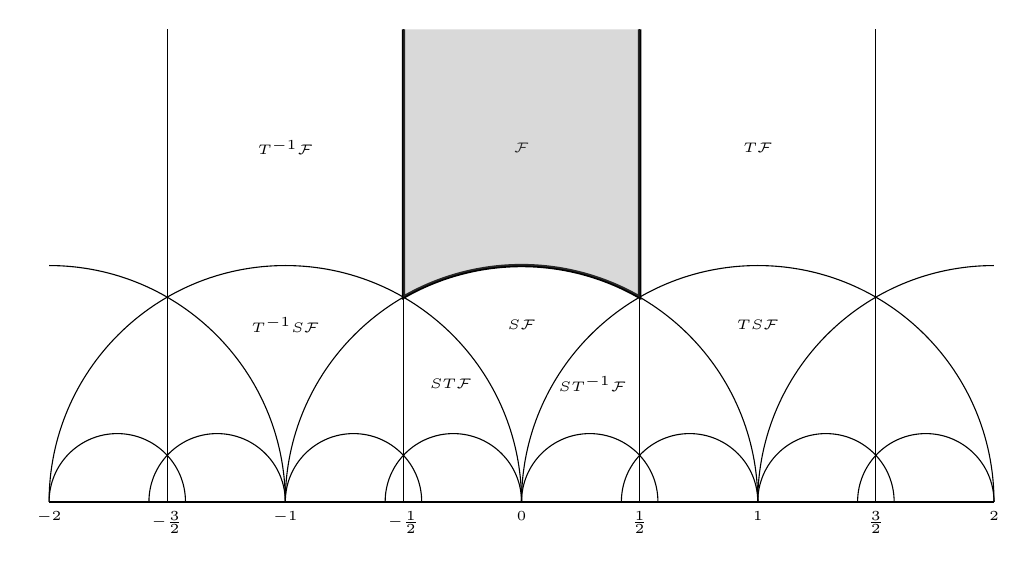
\begin{tikzpicture}[scale=3]
        \def\xmin{-2} \def\xmax{2}
        \def\ymin{0} \def\ymax{2}
        \draw[thick] (\xmin,0) -- (\xmax,0);

        \draw[very thick] (0.5,\ymax) -- (0.5,{sqrt(3)/2}) arc (60:120:1) -- (-0.5,\ymax);

        \node at (-0.5,0) [below] {\tiny{$-\frac{1}{2}$}};
        \node at (0.5,0) [below] {\tiny{$\frac{1}{2}$}};
        \node at (-1.5,0) [below] {\tiny{$-\frac{3}{2}$}};
        \node at (1.5,0) [below] {\tiny{$\frac{3}{2}$}};
        \node at (0,0) [below] {\tiny{$0$}};
        \node at (-1,0) [below] {\tiny{$-1$}};
        \node at (1,0) [below] {\tiny{$1$}};
        \node at (-2,0) [below] {\tiny{$-2$}};
        \node at (2,0) [below] {\tiny{$2$}};

        \draw[thin] (0.5,0) -- (0.5,\ymax);
        \draw[thin] (-0.5,0) -- (-0.5,\ymax);
        \draw[thin] (1.5,0) -- (1.5,\ymax);
        \draw[thin] (-1.5,0) -- (-1.5,\ymax);

        \draw (1,0) arc (0:180:1);
        \draw (-1,0) arc (0:90:1);
        \draw (2,1) arc (90:180:1);

        \draw (0,0) arc (0:180:1);
        \draw (2,0) arc (0:180:1);

        \draw (1,0) arc (0:180:{sqrt(3)/6});
        \draw ({sqrt(3)/3},0) arc (0:180:{sqrt(3)/6});

        \draw (2,0) arc (0:180:{sqrt(3)/6});
        \draw ({1+sqrt(3)/3},0) arc (0:180:{sqrt(3)/6});

        \draw (0,0) arc (0:180:{sqrt(3)/6});
        \draw ({(sqrt(3)/3)-1},0) arc (0:180:{sqrt(3)/6});

        \draw (-1,0) arc (0:180:{sqrt(3)/6});
        \draw ({(sqrt(3)/3)-2},0) arc (0:180:{sqrt(3)/6});

        \node at (0,1.5) {\tiny{$\mc{F}$}};
        \node at (-1,1.5) {\tiny{$T^{-1}\mc{F}$}};
        \node at (1,1.5) {\tiny{$T\mc{F}$}};
        \node at (0,0.75) {\tiny{$S\mc{F}$}};
        \node at (-1,0.75) {\tiny{$T^{-1}S\mc{F}$}};
        \node at (1,0.75) {\tiny{$TS\mc{F}$}};
        \node at (-0.3,0.5) {\tiny{$ST\mc{F}$}};
        \node at (0.3,0.5) {\tiny{$ST^{-1}\mc{F}$}};

        \begin{scope}
          \path[clip] (0.5,\ymax) -- (0.5,{sqrt(3)/2}) arc (60:120:1) -- (-0.5,\ymax) -- cycle;
          \fill[gray,opacity=0.3] (-0.5,0) rectangle (0.5,\ymax);
        \end{scope}
      \end{tikzpicture}
      \caption{The standard fundamental domain for $\PSL_{2}(\Z)\backslash\H$.} \label{fig:fundamental_domain_modular_group}
    \end{figure}
    
    The region $\mc{F}$, shaded in \cref{fig:fundamental_domain_modular_group}, is called the \textbf{standard fundamental domain}\index{standard fundamental domain}. \cref{fig:fundamental_domain_modular_group} also displays how this fundamental domain changes under the actions of the generators of $\PSL_{2}(\Z)$ as in \cref{prop:PSL_generator}. A fundamental domain for any other modular curve can be built from the standard fundamental domain as the following proposition shows (see \cite{kilford2015modular} for a proof):

    \begin{proposition}\label{prop:fundamental_domain_congruence_subgroup}
      Let $\G$ be any congruence subgroup. Then
      \[
        \mc{F}_{\G} = \bigcup_{\g \in \G\backslash\PSL_{2}(\Z)}\g\mc{F},
      \]
      is a fundamental domain for $\G\backslash\H$.
    \end{proposition}

    We might notice that $\mc{F}$ in \cref{fig:fundamental_domain_modular_group} is unbounded as it doesn't contain the point $\infty$. However, if we consider $\mc{F} \cup \{\infty\}$ then it would appear that this space is compact. The point $\infty$ is an example of a cusp and we now make this idea precise. Since any $\g \in \PSL_{2}(\Z)$ preserves $\hat{\R}$ and $\g$ has integer entries, $\g$ also preserves $\Q \cup \{\infty\}$. A \textbf{cusp}\index{cusp} of $\GH$ is an element of of $\G\backslash(\Q \cup \{\infty\})$. As $\G$ has finite index in the modular group, there can only be finitely many cusps and the number of cusps is at most the index of $\G$. In particular, the $\G$-orbit of $\infty$ is a cusp of $\GH$. We denote cusps by gothic characters $\mf{a},\mf{b},\mf{c},\ldots$ or by representatives of their equivalence classes. For example, we let $\infty$ denote the cusp $\G\infty$.

    \begin{remark}
      It turns out that the cusps can be represented as the points needed to make a fundamental domain $\mc{F}_{\G}$ compact as a subset of $\hat{\C}$. To see this, suppose $\mf{a}$ is a limit point of $\mc{F}_{\G}$ that does not belong to $\mc{F}_{\G}$. Then $\mf{a} \in \hat{\R}$. In the case of the standard fundamental domain $\mc{F}$, $\mf{a} = \infty$ which is a cusp. Otherwise, $\mc{F}_{\G}$ is a union of images of $\mc{F}$ by \cref{prop:fundamental_domain_congruence_subgroup} and since $\PSL_{2}(\Z)\infty = \Q \cup \{\infty\}$, we find that $\mf{a} \in \Q \cup \{\infty\}$.
    \end{remark}

    Let $\G_{\mf{a}} \le \G$ denote the stabilizer subgroup of the cusp $\mf{a}$. For the $\infty$ cusp, we can describe $\G_{\infty}$ explicitly. If $\g = \begin{psmallmatrix} a & b \\ c & d \end{psmallmatrix} \in \G$ stabilizes $\infty$, then necessarily $c = 0$ and since $\det(\g) = 1$ we must have $a = d = 1$. Therefore $\g = \begin{psmallmatrix} 1 & b \\ 0 & 1 \end{psmallmatrix}$ for some $b \in \Z$ and $\g$ acts on $\H$ by translation by $b$. Of course, not every translation is guaranteed to belong to $\G$. Letting $t$ be the smallest positive integer such that $\begin{psmallmatrix} 1 & t \\ 0 & 1 \end{psmallmatrix} \in \G$, we have $\G_{\infty} = \left\<\begin{psmallmatrix} 1 & t \\ 0 & 1 \end{psmallmatrix}\right\>$. In particular, $\G_{\infty}$ is an infinite cyclic group. We say that $\G$ is \textbf{reduced at infinity}\index{reduced at infinity} if $t = 1$ so that $\G_{\infty} = \left\<\begin{psmallmatrix} 1 & 1 \\ 0 & 1 \end{psmallmatrix}\right\>$. In particular, $\G_{1}(N)$ and $\G_{0}(N)$ are reduced at infinity.
    
    \begin{remark}
      If $\G$ is of level $N$, then $N$ is the smallest positive integer such that $\G(N) \le \G$ so that $\begin{psmallmatrix} 1 & N \\ 0 & 1 \end{psmallmatrix}$ is the minimal translation guaranteed to belong to $\G$. However, there may be smaller translations so in general $t \le N$.
    \end{remark}
    
    Moreover, for any cusp $\mf{a}$ we have that $\G_{\mf{a}}$ is also an infinite cyclic group and we denote its generator by $\g_{\mf{a}}$. To see this, if $\mf{a} = \frac{a}{c}$ with $(a,c) = 1$ is a cusp of $\GH$ not equivalent to $\infty$, then there exists an $\s_{\mf{a}} \in \PSL_{2}(\Z)$ such that $\s_{\mf{a}}\infty = \mf{a}$. Indeed, there exists integers $d$ and $b$ such that $ad-bc = 1$ by B\'ezout's identity and then $\s_{\mf{a}} = \begin{psmallmatrix} a & b \\ c & d \end{psmallmatrix}$ is such a matrix. It follows that $\G_{\mf{a}} = \s_{\mf{a}}\G_{\infty}\s_{\mf{a}}^{-1}$ and since $\G_{\infty}$ is infinite cyclic so is $\G_{\mf{a}}$. We call any matrix $\s_{\mf{a}} \in \PSL_{2}(\Z)$ satisfying 
    \[
      \s_{\mf{a}}\infty = \mf{a} \quad \text{and} \quad \s_{\mf{a}}^{-1}\g_{\mf{a}}\s_{\mf{a}} = \begin{pmatrix} 1 & t \\ 0 & 1 \end{pmatrix},
    \]
    a \textbf{scaling matrix}\index{scaling matrix} for the cusp $\mf{a}$. Note that $\s_{\mf{a}}$ is determined up to composition on the right by an element of $\G_{\infty}$. Scaling matrices are useful because they allow us to transfer information at the cusp $\mf{a}$ to the cusp at $\infty$. Let $\mf{a}$ and $\mf{b}$ be cusps of $\GH$ with scaling matrices $\s_{\mf{a}}$ and $\s_{\mf{b}}$ respectively. When investigating holomorphic forms, it will be useful to have a double coset decomposition for sets of the form $\s_{\mf{a}}^{-1}\G\s_{\mf{b}}$. This is referred to as the \textbf{Bruhat decomposition}\index{Bruhat decomposition} for $\G$:

    \begin{theorem}[Bruhat decomposition]
      Let $\G$ be any congruence subgroup and let $\mf{a}$ and $\mf{b}$ be cusps of $\GH$ with scaling matrices $\s_{\mf{a}}$ and $\s_{\mf{b}}$ respectively. Then we have the disjoint decomposition
      \[
        \s_{\mf{a}}^{-1}\G\s_{\mf{b}} = \d_{\mf{a},\mf{b}}\W_{\infty}\bigcup_{\substack{c \ge 1 \\ d \tmod{c}}}\W_{d/c},
      \]
      where
      \[
        \W_{\infty} = \G_{\infty}\w_{\infty} = \w_{\infty}\G_{\infty} = \G_{\infty}\w_{\infty}\G_{\infty} \quad \text{and} \quad \W_{d/c} = \G_{\infty}\w_{d/c}\G_{\infty},
      \]
      for some $\w_{\infty} = \begin{psmallmatrix} 1 & \ast \\ 0 & 1 \end{psmallmatrix} \in \s_{\mf{a}}^{-1}\G\s_{\mf{b}}$ and $\w_{d/c} = \begin{psmallmatrix} a & \ast \\ c & d \end{psmallmatrix} \in \s_{\mf{a}}^{-1}\G\s_{\mf{b}}$ with $c \ge 1$ if such a matrix exists otherwise $\W_{d/c}$ is empty. Moreover, the entries $a$ and $d$ of $\w_{d/c}$ are determined modulo $c$.
    \end{theorem}
    \begin{proof}
      We first show that $\W_{\infty}$ is nonempty if and only if $\mf{a} = \mf{b}$. Indeed, if $\w \in \W_{\infty}$ then $\w = \s_{\mf{a}}^{-1}\g\s_{\mf{b}}$ for some $\g \in \G$. Then
      \[
        \g\mf{b} = \s_{\mf{a}}\w\s_{\mf{b}}^{-1}\mf{b} = \s_{\mf{a}}\w\infty = \s_{\mf{a}}\infty = \mf{a}.
      \]
      This shows that $\mf{a} = \mf{b}$. Conversely, suppose $\mf{a} = \mf{b}$. Then $\s_{\mf{a}}^{-1}\G\s_{\mf{b}}$ contains $\s_{\mf{a}}^{-1}\G_{\mf{a}}\s_{\mf{a}} = \G_{\infty}$ so that $\W_{\infty}$ is nonempty. So $\W_{\infty}$ is nonempty if and only if $\mf{a} = \mf{b}$. In this case, for any two elements $\w = \s_{\mf{a}}^{-1}\g\s_{\mf{a}}$ and $\w' = \s_{\mf{a}}^{-1}\g'\s_{\mf{a}}$ of $\W_{\infty}$, we have
      \[
        \g'\g^{-1}\mf{a} = \s_{\mf{a}}\w'\w^{-1}\s_{\mf{a}}^{-1}\mf{a} = \s_{\mf{a}}\w'\w^{-1}\infty = \s_{\mf{a}}\mf{a}.
      \]
      Hence $\g'\g^{-1} \in \G_{\mf{a}}$ which implies $\w'\w^{-1} = \s_{\mf{a}}^{-1}\g'\g^{-1}\s_{\mf{a}} \in \s_{\mf{a}}^{-1}\G_{\mf{a}}\s_{\mf{a}} = \G_{\infty}$. Therefore
      \[
        \W_{\infty} = \G_{\infty}\w = \w\G_{\infty} = \G_{\infty}\w\G_{\infty},
      \]
      where the latter two equalities hold because $\w$ is a translation and translations commute. Every other element of $\s_{\mf{a}}^{-1}\G\s_{\mf{b}}$ belongs to one of the double cosets $\W_{d/c}$ with $c \ge 1$ (since we are working in $\PSL_{2}(\Z)$). The relation
      \[
        \begin{pmatrix} 1 & n \\ 0 & 1 \end{pmatrix}\begin{pmatrix} a & \ast \\ c & d \end{pmatrix}\begin{pmatrix} 1 & m \\ 0 & 1 \end{pmatrix} = \begin{pmatrix} a+cn & \ast \\ c & d+cm \end{pmatrix},
      \]
      shows that $\W_{d/c}$ is determined uniquely by $c$ and $d \tmod{c}$. Moreover, this relation shows that $a$ and $d$ are determined modulo $c$. This completes the proof of the theorem.
    \end{proof}

    Notice that the Bruhat decomposition for $\s_{\mf{a}}^{-1}\G\s_{\mf{b}}$ implies
    \[
      \G_{\infty}\backslash\s_{\mf{a}}^{-1}\G\s_{\mf{b}} = \d_{\mf{a},\mf{b}}\w_{\infty}\bigcup_{\substack{c \ge 1 \\ d \tmod{c}}}\w_{d/c}\G_{\infty},
    \]
    where it is understood that the coset $\w_{d/c}\G_{\infty}$ is empty if the double coset $\W_{d/c}$ is too. This shows that every element of $\G_{\infty}\backslash\s_{\mf{a}}^{-1}\G\s_{\mf{b}}$ corresponds to a unique $(c,d) \in \Z^{2}-\{\mathbf{0}\}$ with $c \ge 1$, $d \in \Z$, and $(c,d) = 1$, and additionally the pair $(0,1)$ if and only if $\mf{a} = \mf{b}$ (this pair corresponds to $\w_{\infty}$). Of course, this correspondence need not be surjective since many of the double cosets $\W_{d/c}$ may be empty. To track such $c$ and $d$ for which $\W_{d/c}$ is nonempty, let $\mc{C}_{\mf{a},\mf{b}}$ and $\mc{D}_{\mf{a},\mf{b}}(c)$ be the sets given by
    \[
      \mc{C}_{\mf{a},\mf{b}} = \left\{c \ge 1: \begin{pmatrix} \ast & \ast \\ c & \ast \end{pmatrix} \in \s_{\mf{a}}^{-1}\G\s_{\mf{b}}\right\} \quad \text{and} \quad \mc{D}_{\mf{a},\mf{b}}(c) = \left\{d \tmod{c}: \begin{pmatrix} \ast & \ast \\ c & d \end{pmatrix} \in \s_{\mf{a}}^{-1}\G\s_{\mf{b}}\right\}.
    \]
    Then $\mc{C}_{\mf{a},\mf{b}}$ and $\mc{D}_{\mf{a},\mf{b}}(c)$ are precisely the sets of $c$ and $d$ take modulo $c$ such that $\W_{d/c}$ is nonempty.

    \begin{remark}\label{rem:Bruhat_modulo_infity_exact}
      The Bruhat decomposition for $\s_{\mf{a}}^{-1}\G\s_{\mf{b}}$ implies
      \[
        \G_{\infty}\backslash\s_{\mf{a}}^{-1}\G\s_{\mf{b}} = \d_{\mf{a},\mf{b}}\w_{\infty}\bigcup_{\substack{c \in \mc{C}_{\mf{a},\mf{b}} \\ d \in \mc{D}_{\mf{a},\mf{b}}(c)}}\w_{d/c}\G_{\infty},
      \]
      where none of the cosets $\w_{d/c}\G_{\infty}$ are empty. In particular, $\g = \begin{psmallmatrix} \ast & \ast \\ c & d \end{psmallmatrix} \in \G_{\infty}\backslash\s_{\mf{a}}^{-1}\G\s_{\mf{b}}$ if and only if $(c,d)$ is a pair with $c \in \mc{C}_{\mf{a},\mf{b}}$, $d \in \Z$, and $d \tmod{c} \in \mc{D}_{\mf{a},\mf{b}}(c)$, or additionally $(0,1)$ if $\mf{a} = \mf{b}$.
    \end{remark}
    
    We will now introduce Kloosterman \& Sali\'e sums associated to cusps. We being with the Kloosterman sums. Let $\s_{\mf{a}}$ and $\s_{\mf{b}}$ be scaling matrices for the cusps $\mf{a}$ and $\mf{b}$ respectively. Then for any $c \in \mc{C}_{\mf{a},\mf{b}}$ and $n,m \in \Z$, the \textbf{generalized Kloosterman sum}\index{generalized Kloosterman sum} $K_{\mf{a},\mf{b}}(n,m,c)$ relative to $\mf{a}$ and $\mf{b}$ is defined by
    \[
      K_{\mf{a},\mf{b}}(n,m,c) = \sum_{d \in \mc{D}_{\mf{a},\mf{b}}(c)}e^{\frac{2\pi i(an+\conj{a}m)}{c}},
    \]
    where $a$ has been determined by $ad-bc = 1$. This sum is well-defined by the Bruhat decomposition because $a$ is determined modulo $c$. In general, $K_{\mf{a},\mf{b}}(n,m,c)$ is not independent of the scaling matrices $\s_{\mf{a}}$ and $\s_{\mf{b}}$. However, if $n = m = 0$ we trivially see by the Bruhat decomposition for $\G$ that
    \[
      K_{\mf{a},\mf{b}}(0,0,c) = \left|\left\{d \tmod{c}:\begin{pmatrix} \ast & \ast \\ c & d \end{pmatrix} \in \s_{\mf{a}}^{-1}\G\s_{\mf{b}}\right\}\right|,
    \]
    which is independent of the scaling matrices $\s_{\mf{a}}$ and $\s_{\mf{b}}$. Moreover, for $\G = \G_{1}(1)$ we have $\mf{a} = \mf{b} = \infty$ and the Bruhat decomposition for $\G_{1}(1)$ implies
    \[
      K_{\infty,\infty}(n,m,c) = K(n,m,c),
    \]
    is the usual Kloosterman sum. Therefore if $\mf{a} = \mf{b} = \infty$, we will suppress these dependencies accordingly. The Sali\'e sums are defined in a similar manner. Let $\s_{\mf{a}}$ and $\s_{\mf{b}}$ be scaling matrices for the cusps $\mf{a}$ and $\mf{b}$ respectively. Then for any $c \in \mc{C}_{\mf{a},\mf{b}}$, and $n,m \in \Z$, and Dirichlet character $\chi$ with conductor $q \mid c$, the \textbf{generalized Sali\'e sum}\index{generalized Sali\'e sum} $S_{\chi,\mf{a},\mf{b}}(n,m,c)$ relative to $\mf{a}$ and $\mf{b}$ is defined by
    \[
      S_{\chi,\mf{a},\mf{b}}(n,m,c) = \sum_{d \in \mc{D}_{\mf{a},\mf{b}}(c)}\chi(a)e^{\frac{2\pi i(an+\conj{a}m)}{c}},
    \]
    where $a$ has been determined by $ad-bc = 1$. This sum is well-defined by the Bruhat decomposition because $a$ is determined modulo $c$. Like the generalized Kloosterman sum, $S_{\mf{a},\mf{b}}(n,m,c)$ need not independent of the scaling matrices $\s_{\mf{a}}$ and $\s_{\mf{b}}$. Moreover, for $\G = \G_{1}(1)$ we have $\mf{a} = \mf{b} = \infty$ and the Bruhat decomposition for $\G_{1}(1)$ implies
    \[
      S_{\chi,\infty,\infty}(n,m,c) = S_{\chi}(n,m,c),
    \]
    is the usual Sali\'e sum. Therefore if $\mf{a} = \mf{b} = \infty$, we will suppress these dependencies accordingly.
  \section{The Hyperbolic Measure}
    We will also need to integrate over $\GH$. In order to do this, we require a measure on $\H$. Our choice of measure will be the \textbf{hyperbolic measure}\index{hyperbolic measure} $d\mu$ given by
    \[
      d\mu = d\mu(z) = \frac{dx\,dy}{y^{2}}.
    \]
    The most important property about the hyperbolic measure is that it is $\GL_{2}^{+}(\R)$-invariant (see \cite{diamond2005first} for a proof):

    \begin{proposition}
      The hyperbolic measure $d\mu$ is $\GL_{2}^{+}(\R)$-invariant.
    \end{proposition}

    As this fact will be used so frequently any time we integrate, we will not mention it explicitly. A particularly important fact is that if $\G$ is a congruence subgroup then $d\mu$ is $\G$-invariant. One of the reasons this is useful is because we can apply the unfolding/folding method to many integrals. The most common instance is when we are integrating the sum $\sum_{\g \in \GG}f(\g z)$ of some holomorphic function $f(z)$ over a fundamental domain $\mc{F}_{\G}$ for $\GH$. Indeed, $\H = \bigcup_{\g \in \G}\g\mc{F}_{\G}$ and so $\G_{\infty}\backslash\H = \bigcup_{\g \in \GG}\g\mc{F}_{\G}$. Since $\mc{F}_{\G}$ is a fundamental domain, the conditions of the unfolding/folding method are satisfied and it follows that
    \[
      \int_{\mc{F}_{\G}}\sum_{\g \in \GG}f(\g z)\,d\mu = \int_{\G_{\infty}\backslash\H}f(z)\,d\mu,
    \]
    provided the sum and or integral on either side are absolutely convergent and absolutely bounded. It is also worth highlighting another fact. Any $\a \in \GL_{2}^{+}(\Q)$ acts as an automorphism of $\H$ which implies that it induces a bijection between $\a^{-1}\G\a\backslash\H$ and $\G\backslash\H$ and hence between the fundamental domains $\mc{F}_{\a^{-1}\G\a}$ and $\mc{F}_{\G}$. Thus the change of variables $z \to \a z$ transforms the fundamental domain $\mc{F}_{\G}$ into $\mc{F}_{\a^{-1}\G\a}$. Therefore
    \[
      \int_{\mc{F}_{\G}}f(z)\,d\mu = \int_{\mc{F}_{\a^{-1}\G\a}}f(\a z)\,d\mu,
    \]
    provided either side is bounded. Now let us discuss the volume of $\GH$. We define the \textbf{volume}\index{volume} $V_{\G}$ of $\GH$ by
    \[
      V_{\G} = \int_{\mc{F}_{\G}}\,d\mu.
    \]
    In other words, $V_{\G}$ is the volume of the fundamental domain $\mc{F}_{\G}$ with respect to the hyperbolic measure. Also, if $\mc{F}_{\G} = \mc{F}$ we write $V_{\G} = V$. Since the integrand is $\G$-invariant, $V_{\G}$ is independent of the choice of fundamental domain. Using \cref{prop:fundamental_domain_modular_group}, we have
    \[
      V = \int_{\mc{F}}\,d\mu = \int_{-\frac{1}{2}}^{\frac{1}{2}}\int_{\sqrt{1-x^{2}}}^{\infty}\frac{dy\,dx}{y^{2}} = \int_{-\frac{1}{2}}^{\frac{1}{2}}\frac{1}{\sqrt{1-x^{2}}}\,dx = \arcsin(x)\bigg|_{-\frac{1}{2}}^{\frac{1}{2}} = \frac{\pi}{3}.
    \]
    Therefore $V$ is finite. There is also a simple relation between $V_{\G}$ and the index of $\G$ in $\PSL_{2}(\Z)$:
    \begin{equation}\label{equ:Petersson_volume_relation}
      V_{\G} = [\PSL_{2}(\Z):\G]V,
    \end{equation}
    which follows immediately from \cref{prop:fundamental_domain_congruence_subgroup}. Moreover, $V_{\G}$ is finite for every congruence subgroup $\G$ by \cref{equ:Petersson_volume_relation} and that congruence subgroups have finite index in the modular group. A particularly nice application of this fact is that any integral of the form
    \[
      \frac{1}{V_{\G}}\int_{\mc{F}_{\G}}f(z)\,d\mu,
    \]
    is bounded by \cref{prop:decay_finite_volume_integral} provided $f(z)$ is holomorphic and bounded. That is, bounded functions are absolutely convergent over $\mc{F}_{\G}$ with respect to $d\mu$. Moreover, we have a useful lemma:

    \begin{lemma}\label{lem:invariance_of_volume}
      Let $\G$ be a congruence subgroup and $\a \in \GL_{2}^{+}(\Q)$. If $\a^{-1}\G\a \subseteq \PSL_{2}(\Z)$, then $V_{\a^{-1}\G\a} = V_{\G}$ and $[\PSL_{2}(\Z):\a^{-1}\G\a] = [\PSL_{2}(\Z):\G]$.
    \end{lemma}
    \begin{proof}
      The first statement follows from the chain
      \[
        V_{\a^{-1}\G\a} = \int_{\mc{F}_{\a^{-1}\G\a}}\,d\mu = \int_{\mc{F}_{\G}}\,d\mu = V_{\G},
      \]
      where the middle equality is justified by making the change of variables $z \to \a^{-1}z$. The second statement is now immediate from \cref{equ:Petersson_volume_relation}.
    \end{proof}
  \chapter{Types of \texorpdfstring{$L$}{L}-functions}
  We discuss a variety of $L$-functions: the Riemann zeta function, $L$-functions attached to Dirichlet characters, and Hecke $L$-functions. In the case of Hecke $L$-functions, we also describe a method of Rankin and Selberg for constructing new $L$-functions from old ones.
  \section{The Riemann Zeta Function}
    \subsection*{The Definition \& Euler Product of \texorpdfstring{$\z(s)$}{\z(s)}}
      The \textbf{Riemann zeta function}\index{Riemann zeta function} $\z(s)$ is defined by the following Dirichlet series:
      \[
        \z(s) = \sum_{n \ge 1}\frac{1}{n^{s}}.
      \]
      This is the prototypical example of a Dirichlet series as all the coefficients are $1$. We will see that $\z(s)$ is a Selberg class $L$-function. As the coefficients are trivially polynomially bounded, $\z(s)$ is locally absolutely uniformly convergent for $\s > 1$. Also note that $\z(s)$ is necessarily nonzero in this region. Determining the Euler product is also an easy matter. As the coefficients are obviously completely multiplicative, we have the degree $1$ Euler product:
      \[
        \z(s) = \prod_{p}(1-p^{-s})^{-1},
      \]
      in this region as well. The local factor at $p$ is $\z_{p}(s) = (1-p^{-s})^{-1}$ with local root $1$.
    \subsection*{The Integral Representation of \texorpdfstring{$\z(s)$}{\z(s)}: Part I}
      We want to find an integral representation for $\z(s)$. To do this, consider the function
      \[
        \w(z) = \sum_{n \ge 1}e^{\pi in^{2}z},
      \]
      defined for $z \in \H$. It is locally absolutely uniformly convergent in this region by the ratio test. Moreover, from the Taylor series of $\frac{1}{1-e^{y}}$ we see that
      \[
        \w(z) = O\left(\sum_{n \ge 1}e^{-\pi n^{2}y}\right) = O\left(\sum_{n \ge 1}e^{-\pi ny}\right) = O\left(\frac{1}{1-e^{-\pi y}}\right) = O(e^{-\pi y}),
      \]
      and so $\w$ exhibits rapid decay. Now consider the following Mellin transform:
      \[
        \int_{0}^{\infty}\w(iy)y^{\frac{s}{2}}\,\frac{dy}{y}.
      \]
      By the rapid decay of $\w$, this integral exists and defines an analytic function for $\s > 1$. Then we compute
      \begin{align*}
        \int_{0}^{\infty}\w(iy)y^{\frac{s}{2}}\,\frac{dy}{y} &= \int_{0}^{\infty}\sum_{n \ge 1}e^{-\pi n^{2}y}y^{\frac{s}{2}}\,\frac{dy}{y} \\
        &= \sum_{n \ge 1}\int_{0}^{\infty}e^{-\pi n^{2}y}y^{\frac{s}{2}}\,\frac{dy}{y} && \text{DCT} \\
        &= \sum_{n \ge 1}\frac{1}{\pi^{\frac{s}{2}}n^{s}}\int_{0}^{\infty}e^{-y}y^{\frac{s}{2}}\,\frac{dy}{y} && \text{$y \to \frac{y}{\pi n^{2}}$} \\
        &= \frac{\G\left(\frac{s}{2}\right)}{\pi^{\frac{s}{2}}}\sum_{n \ge 1}\frac{1}{n^{s}} \\
        &= \frac{\G\left(\frac{s}{2}\right)}{\pi^{\frac{s}{2}}}\z(s).
      \end{align*}
      Therefore we have an integral representation
      \begin{equation}\label{equ:integral_representation_zeta_1}
        \z(s) = \frac{\pi^{\frac{s}{2}}}{\G\left(\frac{s}{2}\right)}\int_{0}^{\infty}\w(iy)y^{\frac{s}{2}}\,\frac{dy}{y}.
      \end{equation}
      Unfortunately, we cannot proceed until we obtain a functional equation for $\w$. So we will make a slight detour and come back to the integral representation after.
    \subsection*{Jacobi's Theta Function \texorpdfstring{$\vt(z)$}{\vt(z)}}
      \textbf{Jacobi's theta function}\index{Jacobi's theta function} $\vt(z)$ is defined by
      \[
        \vt(z) = \sum_{n \in \Z}e^{2\pi in^{2}z},
      \]
      for $z \in \H$. Its relation to $\w$ is given by the identity
      \begin{equation}\label{equ:omega_theta_relationship_for_zeta}
        \w(z) = \frac{\vt\left(\frac{z}{2}\right)-1}{2},
      \end{equation}
      and so $\vt$ is locally absolutely uniformly convergent in this region and exhibits rapid decay. The essential we will need is the \textbf{functional equation for Jacobi's theta function}\index{functional equation for Jacobi's theta function}:

      \begin{theorem}[Functional equation for Jacobi's theta function]
        For $z \in \H$,
        \[
          \vt(z) = \frac{1}{\sqrt{-2iz}}\vt\left(-\frac{1}{4z}\right).
        \]
      \end{theorem}
      \begin{proof}
        By the identity theorem it suffices to verify this for $z = iy$ with $y > 0$. So set $f(x) = e^{-2\pi x^{2}y}$. Then $f(x)$ is of Schwarz class. We compute its Fourier transform:
        \[
          \hat{f}(t) = \int_{-\infty}^{\infty}f(x)e^{-2\pi itx}\,dx = \int_{-\infty}^{\infty}e^{-2\pi x^{2}y}e^{-2\pi itx}\,dx = \int_{-\infty}^{\infty}e^{-2\pi(x^{2}y+itx)}\,dx.
        \]
        Making the change of variables $x \to \frac{x}{\sqrt{y}}$, the last integral above becomes
        \[
          \frac{1}{\sqrt{y}}\int_{-\infty}^{\infty}e^{-2\pi\left(x^{2}+\frac{itx}{\sqrt{y}}\right)}.
        \]
        Complete the square in the exponent by noticing
        \[
          -2\pi\left(x^{2}+\frac{itx}{\sqrt{y}}\right) = -2\pi\left(\left(x+\frac{it}{2\sqrt{y}}\right)^{2}+\frac{t^{2}}{4y}\right).
        \]
        Taking exponentials, this implies that the previous integral is equal to
        \[
          \frac{e^{-\frac{\pi t^{2}}{2y}}}{\sqrt{y}}\int_{-\infty}^{\infty}e^{-2\pi\left(x+\frac{it}{2\sqrt{y}}\right)^{2}}\,dx.
        \]
        The change of variables $x \to \frac{x}{\sqrt{2}}-\frac{it}{2\sqrt{y}}$ is permitted without affecting the line of integration by viewing the integral as a complex integral, noting that the integrand is entire as a complex function, and shifting the line of integration. This gives
        \[
          \frac{e^{-\frac{\pi t^{2}}{2y}}}{\sqrt{2y}}\int_{-\infty}^{\infty}e^{-\pi x^{2}}\,dx = \frac{e^{-\frac{\pi t^{2}}{2y}}}{\sqrt{2y}},
        \]
        where the last equality follows because the last integral above is $1$ since it is the Gaussian integral (see \cref{append:Special_Integrals}). Thus
        \[
          \hat{f}(t) = \frac{e^{-\frac{\pi t^{2}}{2y}}}{\sqrt{2y}}.
        \]
        By the Poisson summation formula, we have
        \[
          \vt(iy) = \sum_{t \in \Z}\frac{e^{-\frac{\pi t^{2}}{2y}}}{\sqrt{2y}} = \frac{1}{\sqrt{2y}}\sum_{t \in \Z}e^{-\frac{\pi t^{2}}{2y}} = \frac{1}{\sqrt{2y}}\vt\left(-\frac{1}{4iy}\right),
        \]
        and the identity theorem finishes the proof.
      \end{proof}

      We will use this functional equation to analytically continue $\z(s)$.
    \subsection*{The Integral Representation of \texorpdfstring{$\z(s)$}{\z(s)}: Part II}
      Returning to the Riemann zeta function, we split the integral in \cref{equ:integral_representation_zeta_1} into two pieces
      \begin{equation}\label{equ:symmetric_integral_zeta_split}
        \int_{0}^{\infty}\w(iy)y^{\frac{s}{2}}\,\frac{dy}{y} = \int_{0}^{1}\w(iy)y^{\frac{s}{2}}\,\frac{dy}{y}+\int_{1}^{\infty}\w(iy)y^{\frac{s}{2}}\,\frac{dy}{y}.
      \end{equation}
      The idea now is to rewrite the first piece in the same form and symmetrize the result as much as possible. We being by performing a change of variables $y \to \frac{1}{y}$ to the first piece to obtain
      \[
        \int_{1}^{\infty}\w\left(\frac{i}{y}\right)y^{-\frac{s}{2}}\,\frac{dy}{y}
      \]
      Now the functional equation for Jacobi's theta function $\vt$ and \cref{equ:omega_theta_relationship_for_zeta} together imply
      \begin{align*}
        \w\left(\frac{i}{y}\right) &= \w\left(-\frac{1}{iy}\right) \\
        &= \frac{\vt\left(-\frac{1}{2iy}\right)-1}{2} \\
        &= \frac{\sqrt{y}\vt\left(\frac{iy}{2}\right)-1}{2} \\
        &= \frac{\sqrt{y}(2\w(iy)+1)-1}{2} \\
        &= \sqrt{y}\w(iy)+\frac{\sqrt{y}}{2}-\frac{1}{2}.
      \end{align*}
      This relation gives the first equality in the following chain:
      \begin{align*}
        \int_{1}^{\infty}\w\left(\frac{1}{y}\right)y^{-\frac{s}{2}}\,\frac{dy}{y} &= \int_{1}^{\infty}\left(\sqrt{y}\w(iy)+\frac{\sqrt{y}}{2}-\frac{1}{2}\right)y^{-\frac{s}{2}}\,\frac{dy}{y} \\
        &= \int_{1}^{\infty}\w(iy)y^{\frac{1-s}{2}}\,\frac{dy}{y}+\int_{1}^{\infty}\frac{x^{\frac{1-s}{2}}}{2}\,\frac{dy}{y}-\int_{1}^{\infty}\frac{y^{-\frac{s}{2}}}{2}\,\frac{dy}{y} \\
        &= \int_{1}^{\infty}\w(iy)y^{\frac{1-s}{2}}\,\frac{dy}{y}+\frac{1}{1-s}-\frac{1}{s} \\
        &= \int_{1}^{\infty}\w(iy)y^{\frac{1-s}{2}}\,\frac{dy}{y}-\frac{1}{s(1-s)}.
      \end{align*}
      Substituting this result back into \cref{equ:symmetric_integral_zeta_split} with \cref{equ:integral_representation_zeta_1} yields the integral representation
      \[
        \z(s) = \frac{\pi^{\frac{s}{2}}}{\G\left(\frac{s}{2}\right)}\left[-\frac{1}{s(1-s)}+\int_{1}^{\infty}\w(iy)y^{\frac{1-s}{2}}\,\frac{dy}{y}+\int_{1}^{\infty}\w(iy)y^{\frac{s}{2}}\,\frac{dy}{y}\right].
      \]
      This integral representation will give analytic continuation. To see this, first observe that everything outside the brackets is entire. Moreover, the two integrals are locally absolutely uniformly convergent on $\C$ by \cref{prop:decay_unbounded_inteval_integral}. The fractional term is holomorphic except for simple poles at $s = 0$ and $s = 1$. The meromorphic continuation to $\C$ follows with possible simple poles at $s = 0$ and $s = 1$. There is no pole at $s = 0$. Indeed, $\g(s,\z)$ has a simple pole coming from the gamma factor there and so its reciprocal has a simple zero. This cancels the corresponding simple pole of $\frac{1}{s(1-s)}$ so that $\z(s)$ has a removable singularity and thus is holomorphic at $s = 0$. At $s = 1$, $\g(s,\z)$ is nonzero, and so $\z(s)$ has a simple pole. Therefore $\z(s)$ has meromorphic continuation to all of $\C$ with a simple pole at $s = 1$. 
    \subsection*{The Functional Equation, Critical Strip \& Residue of \texorpdfstring{$\z(s)$}{\z(s)}}
      An immediate consequence of applying the symmetry $s \to 1-s$ to the integral representation is the following functional equation:
      \[
        \frac{\G\left(\frac{s}{2}\right)}{\pi^{\frac{s}{2}}}\z(s) = \frac{\G\left(\frac{1-s}{2}\right)}{\pi^{\frac{1-s}{2}}}\z(1-s).
      \]
      We identify the gamma factor as
      \[
        \g(s,\z) = \pi^{-\frac{s}{2}}\G\left(\frac{s}{2}\right),
      \]
      with $\k = 0$ the only local root at infinity. Clearly it satisfies the required bounds. The conductor is $q(\z) = 1$ so no primes ramify. The completed Riemann zeta function is
      \[
        \L(s,\z) = \pi^{-\frac{s}{2}}\G\left(\frac{s}{2}\right)\z(s),
      \]
      with functional equation
      \[
        \L(s,\z) = \L(1-s,\z).
      \]
      This is the functional equation of $\z(s)$ and in this case is just a reformulation of the previous functional equation. From it we find that the root number is $\e(\z) = 1$ and that $\z(s)$ is self-dual. We can now show that the order of $\z(s)$ is $1$. As there is only a simple pole at $s = 1$, multiply by $(s-1)$ to clear the polar divisor. As the integrals in the integral representation are locally absolutely uniformly convergent, computing the order amounts to estimating the gamma factor. Since the reciprocal of the gamma function is of order $1$, we have
      \[
        \frac{1}{\g(s,\z)} \ll_{\e} e^{|s|^{1+\e}}.
      \]
      Thus the reciprocal of the gamma factor is also of order $1$. It follows that
      \[
        (s-1)\z(s) \ll_{\e} e^{|s|^{1+\e}}.
      \]
      This shows $(s-1)\z(s)$ is of order $1$, and thus $\z(s)$ is as well after removing the polar divisor. We now compute the residue of $\z(s)$ at $s = 1$:

      \begin{proposition}\label{prop:zeta_residue}
        \[
          \Res_{s = 1}\z(s) = 1.
        \]
      \end{proposition}
      \begin{proof}
        The only term in the integral representation of $\z(s)$ contributing to the pole is $-\frac{\pi^{\frac{s}{2}}}{\G\left(\frac{s}{2}\right)}\frac{1}{s(1-s)}$. Observe
        \[
          \lim_{s \to 1}\frac{\pi^{\frac{s}{2}}}{\G\left(\frac{s}{2}\right)} = 1,
        \]
        because $\G\left(\frac{1}{2}\right) = \sqrt{\pi}$. Therefore
        \[
          \Res_{s = 1}\z(s) = \Res_{s = 1}-\frac{\pi^{\frac{s}{2}}}{\G\left(\frac{s}{2}\right)}\frac{1}{s(1-s)} = \Res_{s = 1}-\frac{1}{s(1-s)} = \lim_{s \to 1}-\frac{(s-1)}{s(1-s)} = 1.
        \]
      \end{proof}

      We summarize all of our work into the following theorem:

      \begin{theorem}\label{thm:zeta_Selberg}
        $\z(s)$ is a Selberg class $L$-function. For $\s > 1$, it has a degree $1$ Euler product given by
        \[
          \z(s) = \prod_{p}(1-p^{-s})^{-1}.
        \]
        Moreover, it admits meromorphic continuation to $\C$ via the integral representation
        \[
          \z(s) = \frac{\pi^{\frac{s}{2}}}{\G\left(\frac{s}{2}\right)}\left[-\frac{1}{s(1-s)}+\int_{1}^{\infty}\w(iy)y^{\frac{1-s}{2}}\,\frac{dy}{y}+\int_{1}^{\infty}\w(iy)y^{\frac{s}{2}}\,\frac{dy}{y}\right],
        \]
        with functional equation
        \[
          \pi^{-\frac{s}{2}}\G\left(\frac{s}{2}\right)\z(s) = \L(s,\z) = \L(1-s,\z),
        \]
        and there is a simple pole at $s = 1$ of residue $1$.
      \end{theorem}

      Lastly, we note that by virtue of the functional equation we can also compute $\z(0)$. Indeed, since $\Res_{s = 1}\z(s) = 1$, we have
      \[
        \lim_{s \to 1}(s-1)\L(s,\z) = \Res_{s = 1}\z(s)\lim_{s \to 1}\pi^{-\frac{s}{2}}\G\left(\frac{s}{2}\right) = 1.
      \]
      In other words, $\L(s,\z)$ has a simple pole at $s = 1$ with residue $1$ too. Since the completed Riemann zeta function is completely symmetric as $s \to 1-s$, it has a simple pole at $s = 0$ with residue $1$. Hence
      \[
        1 = \lim_{s \to 1}(s-1)\L(1-s,\z) = \Res_{s = 1}\G\left(\frac{1-s}{2}\right)\lim_{s \to 1}\pi^{-\frac{1-s}{2}}\z(1-s) = -2\z(0),
      \]
      because $\Res_{s = 0}\G(s) = 1$. Therefore $\z(0) = -\frac{1}{2}$.
  \section{Dirichlet \texorpdfstring{$L$}{L}-functions}
    \subsection*{The Definition \& Euler Product of \texorpdfstring{$L(s,\chi)$}{L(s,\chi)}}
      To every Dirichlet character $\chi$ there is an associated $L$-function. Throughout we will let $m$ denote the modulus and $q$ the conductor of $\chi$ respectively. The \textbf{Dirichlet $L$-series}\index{Dirichlet $L$-series} (respectively \textbf{Dirichlet $L$-function}\index{Dirichlet $L$-function} if it is an $L$-function) $L(s,\chi)$ attached to the Dirichlet character $\chi$ is defined by the following Dirichlet series:
      \[
        L(s,\chi) = \sum_{n \ge 1}\frac{\chi(n)}{n^{s}}.
      \]
      Since $\chi(n) = 0$ if $(n,m) > 1$, the above sum can be restricted to all positive integers relatively prime to $m$. We will see that $L(s,\chi)$ is a Selberg class $L$-function if $\chi$ is primitive and of conductor $q > 1$ (in the case $q = 1$, $L(s,\chi) = \z(s)$). From now we make this assumption about $\chi$. As $|\chi(n)| \ll 1$, $L(s,\chi)$ is locally absolutely uniformly convergent for $\s > 1$. Because $\chi$ is completely multiplicative we also have the degree $1$ Euler product:
      \[
        L(s,\chi) = \prod_{p}(1-\chi(p)p^{-s})^{-1} = \prod_{p \nmid m}(1-\chi(p)p^{-s})^{-1},
      \]
      in this region as well. The last equality holds because if $p \mid m$ we have $\chi(p) = 0$. So for $p \mid m$, the local factor at $p$ is $L_{p}(s,\chi) = 1$ with local root $0$. For $p \nmid m$ the local factor at $p$ is $L_{p}(s,\chi) = (1-\chi(p)p^{-s})^{-1}$ with local root $\chi(p)$.
    \subsection*{The Integral Representation of \texorpdfstring{$L(s,\chi)$}{L(s,\chi)}: Part I}
      The integral representation for $L(s,\chi)$ is deduced in a similar way as for $\z(s)$. However, it will depend on if $\chi$ is even or odd. To handle both cases simultaneously let $\mf{a} = 0,1$ according to whether $\chi$ is even or odd. In other words,
      \[
        \mf{a} = \frac{\chi(1)-\chi(-1)}{2}.
      \]
      We also have $\chi(-1) = (-1)^{\mf{a}}$. Note that $\mf{a}$ takes the same value for both $\chi$ and $\cchi$. To find an integral representation for $L(s,\chi)$, consider the function
      \[
        \w_{\chi}(z) = \sum_{n \ge 1}\chi(n)n^{\mf{a}}e^{\pi in^{2}z},
      \]
      defined for $z \in \H$. It is locally absolutely uniformly convergent in this region by the ratio test. From the Taylor series of $\frac{1}{1-e^{y}}$ and its derivative, we have
      \[
        \w_{\chi}(z) = O\left(\sum_{n \ge 1}ne^{-\pi n^{2}y}\right) = O\left(\sum_{n \ge 1}ne^{-\pi ny}\right) = O\left(\frac{e^{-\pi y}}{(1-e^{-\pi y})^{2}}\right) = O(e^{-\pi y}),
      \]
      and thus $\w_{\chi}$ exhibits rapid decay. Now consider the following Mellin transform:
      \[
        \int_{0}^{\infty}\w_{\chi}(iy)y^{\frac{s+\mf{a}}{2}}\,\frac{dy}{y}.
      \]
      By the rapid decay of $w_{\chi}$, this integral exists and defines an analytic function for $\s > 1$. Then we compute
      \begin{align*}
        \int_{0}^{\infty}\w_{\chi}(iy)y^{\frac{s+\mf{a}}{2}}\,\frac{dy}{y} &= \int_{0}^{\infty}\sum_{n \ge 1}\chi(n)n^{\mf{a}}e^{-\pi n^{2}y}y^{\frac{s+\mf{a}}{2}}\,\frac{dy}{y} \\
        &= \sum_{n \ge 1}\int_{0}^{\infty}\chi(n)n^{\mf{a}}e^{-\pi n^{2}y}y^{\frac{s+\mf{a}}{2}}\,\frac{dy}{y} && \text{DCT} \\
        &= \sum_{n \ge 1}\frac{\chi(n)}{\pi^{\frac{s+\mf{a}}{2}}n^{s}}\int_{0}^{\infty}e^{-y}y^{\frac{s+\mf{a}}{2}}\,\frac{dy}{y} && \text{$y \to \frac{y}{\pi n^{2}}$} \\
        &= \frac{\G\left(\frac{s+\mf{a}}{2}\right)}{\pi^{\frac{s+\mf{a}}{2}}}\sum_{n \ge 1}\frac{\chi(n)}{n^{s}} \\
        &= \frac{\G\left(\frac{s+\mf{a}}{2}\right)}{\pi^{\frac{s+\mf{a}}{2}}}L(s,\chi).
      \end{align*}
      Therefore we have an integral representation
      \begin{equation}\label{equ:integral_representation_Dirichlet_L-functions_1}
        L(s,\chi) = \frac{\pi^{\frac{s+\mf{a}}{2}}}{\G\left(\frac{s+\mf{a}}{2}\right)}\int_{0}^{\infty}\w_{\chi}(iy)y^{\frac{s+\mf{a}}{2}}\,\frac{dy}{y},
      \end{equation}
      and just as for the Riemann zeta function, we need to find a functional equation for $\w_{\chi}$ before we can proceed.
    \subsection*{Dirichlet's Theta Function \texorpdfstring{$\vt_{\chi}(z)$}{\vt_{\chi}(z)}}
      \textbf{Dirichlet's theta function}\index{Dirichlet's theta function} $\vt_{\chi}(z)$ attached to the character $\chi$, is defined by
      \[
        \vt_{\chi}(z) = \sum_{n \in \Z}\chi(n)n^{\mf{a}}e^{2\pi in^{2}z},
      \]
      for $z \in \H$. The relationship to $\w_{\chi}$ is
      \begin{equation}\label{equ:twisted_omega_theta_relationship_for_Dirichlet_L-functions}
        \w_{\chi}(z) = \frac{\vt_{\chi}\left(\frac{z}{2}\right)}{2},
      \end{equation}
      and so $\vt_{\chi}$ is locally absolutely uniformly convergent in this region and exhibits rapid decay.

      \begin{remark}
        \cref{equ:twisted_omega_theta_relationship_for_Dirichlet_L-functions} is a slightly less complex relationship than \cref{equ:omega_theta_relationship_for_zeta}. This is because assuming $q > 1$ means $\chi(0) = 0$.
      \end{remark}

      The essential fact we will need is the \textbf{functional equation for Dirichlet's theta function}\index{functional equation for Dirichlet's theta function}:

      \begin{theorem}[Functional equation for Dirichlet's theta function]
        Let $\chi$ be a primitive Dirichlet character of conductor $q > 1$. For $z \in \H$,
        \[
          \vt_{\chi}(z) = \frac{\e_{\chi}}{i^{\mf{a}}(-2qiz)^{\frac{1}{2}+\mf{a}}}\vt_{\cchi}\left(-\frac{1}{4q^{2}z}\right).
        \]
      \end{theorem}
      \begin{proof}
        By the identity theorem it suffices to verify this for $z = iy$ with $y > 0$. Since $\chi$ is $q$-periodic and $\vt_{\chi}$ is absolutely convergent, we can write
        \[
          \vt_{\chi}(iy) = \sum_{a \tmod{q}}\chi(a)\sum_{m \in \Z}(mq+a)^{\mf{a}}e^{-2\pi(mq+a)^{2}y}.
        \]
        Set $f(x) = (xq+a)^{\mf{a}}e^{-2\pi(xq+a)^{2}y}$. Then $f(x)$ is of Schwarz class. We compute its Fourier transform:
        \[
          \hat{f}(t) = \int_{-\infty}^{\infty}f(x)e^{-2\pi itx}\,dx = \int_{-\infty}^{\infty}(xq+a)^{\mf{a}}e^{-2\pi(xq+a)^{2}y}e^{-2\pi itx}\,dx = \int_{-\infty}^{\infty}(xq+a)^{\mf{a}}e^{-2\pi((xq+a)^{2}y+itx)}\,dx.
        \]
        By performing the change of variables $x \to \frac{x}{q\sqrt{y}}-\frac{a}{q}$, the last integral above becomes
        \[
          \frac{e^{\frac{2\pi iat}{q}}}{qy^{\frac{1+\mf{a}}{2}}}\int_{-\infty}^{\infty}x^{\mf{a}}e^{-2\pi\left(x^{2}+\frac{itx}{q\sqrt{y}}\right)}\,dx.
        \]
        Complete the square in the exponent by observing
        \[
          -2\pi\left(x^{2}+\frac{itx}{q\sqrt{y}}\right) = -2\pi\left(\left(x+\frac{it}{2q\sqrt{y}}\right)^{2}+\frac{t^{2}}{4q^{2}y}\right).
        \]
        Taking exponentials, this implies that the previous integral is equal to
        \[
          \frac{e^{\frac{2\pi iat}{q}-\frac{\pi t^{2}}{2q^{2}y}}}{qy^{\frac{1+\mf{a}}{2}}}\int_{-\infty}^{\infty}x^{\mf{a}}e^{-2\pi\left(x+\frac{it}{2q\sqrt{y}}\right)^{2}}\,dx.
        \]
        The change of variables $x \to \frac{x}{\sqrt{2}}-\frac{it}{2q\sqrt{y}}$ is permitted without affecting the line of integration by viewing the integral as a complex integral, noting that the integrand is entire as a complex function, and shifting the line of integration. This gives
        \[
          \frac{e^{\frac{2\pi iat}{q}-\frac{\pi t^{2}}{2q^{2}y}}}{\sqrt{2}qy^{\frac{1+\mf{a}}{2}}}\int_{-\infty}^{\infty}\left(\frac{x}{\sqrt{2}}-\frac{it}{2q\sqrt{y}}\right)^{\mf{a}}e^{-\pi x^{2}}\,dx = \frac{e^{\frac{2\pi iat}{q}-\frac{\pi t^{2}}{2q^{2}y}}}{\sqrt{2}qy^{\frac{1+\mf{a}}{2}}}\int_{-\infty}^{\infty}\left(\frac{x}{\sqrt{2}}+\frac{t}{2qi\sqrt{y}}\right)^{\mf{a}}e^{-\pi x^{2}}\,dx.
        \]
        If $\mf{a} = 0$, we obtain
        \begin{equation}\label{transformation_law_for_twisted_Jacobi's_theta_function_1}
          \frac{e^{\frac{2\pi iat}{q}-\frac{\pi t^{2}}{2q^{2}y}}}{\sqrt{2}qy^{\frac{1+\mf{a}}{2}}}\int_{-\infty}^{\infty}e^{-\pi x^{2}}\,dx = \frac{e^{\frac{2\pi iat}{q}-\frac{\pi t^{2}}{2q^{2}y}}}{\sqrt{2}qy^{\frac{1+\mf{a}}{2}}},
        \end{equation}
        where the equality holds because the integral is $1$ since it is the Gaussian integral (see \cref{append:Special_Integrals}). If $\mf{a} = 1$, then by direct computation
        \[
          \int_{-\infty}^{\infty}\frac{x}{\sqrt{2}}e^{-\pi x^{2}}\,dx = -\frac{1}{\sqrt{8}\pi}e^{-\pi x^{2}}\bigg|_{-\infty}^{\infty} = 0,
        \]
        and
        \begin{equation}\label{transformation_law_for_twisted_Jacobi's_theta_function_2}
          \frac{e^{\frac{2\pi iat}{q}-\frac{\pi t^{2}}{2q^{2}y}}}{\sqrt{2}qy^{\frac{1+\mf{a}}{2}}}\int_{-\infty}^{\infty}\left(\frac{t}{2qi\sqrt{y}}\right)e^{-\pi x^{2}}\,dx = \frac{e^{\frac{2\pi iat}{q}-\frac{\pi t^{2}}{2q^{2}y}}}{\sqrt{2}qy^{\frac{1+\mf{a}}{2}}}\left(\frac{t}{2qi\sqrt{y}}\right)\int_{-\infty}^{\infty}e^{-\pi x^{2}}\,dx = \frac{e^{\frac{2\pi iat}{q}-\frac{\pi t^{2}}{2q^{2}y}}}{\sqrt{2}qy^{\frac{1+\mf{a}}{2}}}\left(\frac{t}{2qi\sqrt{y}}\right),
        \end{equation}
        where the last equality follows because the last integral is the Gaussian integral again. Since $\left(\frac{t}{2qi\sqrt{y}}\right)^{\mf{a}} = 1$ if $\mf{a} = 0$, \cref{transformation_law_for_twisted_Jacobi's_theta_function_1,transformation_law_for_twisted_Jacobi's_theta_function_2} together imply
        \[
          \hat{f}(t) = \frac{e^{\frac{2\pi iat}{q}-\frac{\pi t^{2}}{2q^{2}y}}}{\sqrt{2}qy^{\frac{1+\mf{a}}{2}}}\left(\frac{t}{2qi\sqrt{y}}\right)^{\mf{a}}.
        \]
        By the Poisson summation formula, we have
        \begin{align*}
          \vt_{\chi}(iy) &= \sum_{a \tmod{q}}\chi(a)\sum_{t \in \Z}\frac{e^{\frac{2\pi iat}{q}-\frac{\pi t^{2}}{2q^{2}y}}}{\sqrt{2}qy^{\frac{1+\mf{a}}{2}}}\left(\frac{t}{2qi\sqrt{y}}\right)^{\mf{a}} \\
          &= \frac{1}{i^{\mf{a}}q^{1+\mf{a}}(2y)^{\frac{1}{2}+\mf{a}}}\sum_{a \tmod{q}}\chi(a)\sum_{t \in \Z}t^{\mf{a}}e^{\frac{2\pi iat}{q}-\frac{\pi t^{2}}{2q^{2}y}} \\
          &= \frac{1}{i^{\mf{a}}q^{1+\mf{a}}(2y)^{\frac{1}{2}+\mf{a}}}\sum_{t \in \Z}t^{\mf{a}}e^{-\frac{\pi t^{2}}{2q^{2}y}}\sum_{a \tmod{q}}\chi(a)e^{\frac{2\pi i at}{q}} \\
          &= \frac{1}{i^{\mf{a}}q^{1+\mf{a}}(2y)^{\frac{1}{2}+\mf{a}}}\sum_{t \in \Z}t^{\mf{a}}e^{-\frac{\pi t^{2}}{2q^{2}y}}\tau(t,\chi) && \text{definition of $\tau(t,\chi)$} \\
          &= \frac{\tau(\chi)}{i^{\mf{a}}q^{1+\mf{a}}(2y)^{\frac{1}{2}+\mf{a}}}\sum_{t \in \Z}\cchi(t)t^{\mf{a}}e^{-\frac{\pi t^{2}}{2q^{2}y}} && \text{\cref{cor:gauss_sum_primitive_formula}} \\
          &= \frac{\e_{\chi}}{i^{\mf{a}}(2qy)^{\frac{1}{2}+\mf{a}}}\sum_{t \in \Z}\cchi(t)t^{\mf{a}}e^{-\frac{\pi t^{2}}{2q^{2}y}} && \text{$\e_{\chi} = \frac{\tau(\chi)}{\sqrt{q}}$} \\
          &=  \frac{\e_{\chi}}{i^{\mf{a}}(2qy)^{\frac{1}{2}+\mf{a}}}\vt_{\cchi}\left(-\frac{1}{4q^{2}iy}\right),
        \end{align*}
        and the identity theorem finishes the proof.
      \end{proof}
      Notice that the functional equation relates $\vt_{\chi}$ to $\vt_{\cchi}$. Regardless, we will use it to analytically continue $L(s,\chi)$.
    \subsection*{The Integral Representation of \texorpdfstring{$L(s,\chi)$}{L(s,\chi)}: Part II}
      Returning to $L(s,\chi)$, split the integral in \cref{equ:integral_representation_Dirichlet_L-functions_1} into two pieces
      \begin{equation}\label{equ:symmetric_integral_Dirichlet_L-functions_split}
        \int_{0}^{\infty}\w_{\chi}(iy)y^{\frac{s+\mf{a}}{2}}\,\frac{dy}{y} = \int_{0}^{\frac{1}{q}}\w_{\chi}(iy)y^{\frac{s+\mf{a}}{2}}\,\frac{dy}{y}+\int_{\frac{1}{q}}^{\infty}\w_{\chi}(iy)y^{\frac{s+\mf{a}}{2}}\,\frac{dy}{y}.
      \end{equation}
      We now rewrite the first piece in the same form and symmetrize the result as much as possible. Start by performing a change of variables $y \to \frac{1}{q^{2}y}$ to the first piece to obtain
      \[
        q^{-(s+\mf{a})}\int_{\frac{1}{q}}^{\infty}\w_{\chi}\left(\frac{i}{q^{2}y}\right)y^{-\frac{s+\mf{a}}{2}}\,\frac{dy}{y}.
      \]
      Now the functional equation for Dirichlet's theta function and \cref{equ:twisted_omega_theta_relationship_for_Dirichlet_L-functions} together imply
      \begin{align*}
        \w_{\chi}\left(\frac{i}{q^{2}y}\right) &= \w_{\chi}\left(-\frac{1}{q^{2}iy}\right) \\
        &= \frac{\vt_{\chi}\left(-\frac{1}{2q^{2}iy}\right)}{2} \\
        &= \frac{i^{\mf{a}}(qy)^{\frac{1}{2}+\mf{a}}}{\e_{\cchi}}\frac{\vt_{\cchi}\left(\frac{iy}{2}\right)}{2} \\
        &= \frac{i^{\mf{a}}(qy)^{\frac{1}{2}+\mf{a}}}{\e_{\cchi}}\frac{\vt_{\cchi}\left(\frac{iy}{2}\right)}{2} \\
        &= \e_{\chi}(-i)^{\mf{a}}(qy)^{\frac{1}{2}+\mf{a}}\frac{\vt_{\cchi}\left(\frac{iy}{2}\right)}{2} && \text{\cref{prop:epsilon_factor_relationship} and $\chi(-1) = (-1)^{\mf{a}}$} \\
        &= \frac{\e_{\chi}(qy)^{\frac{1}{2}+\mf{a}}}{i^{\mf{a}}}\frac{\vt_{\cchi}\left(\frac{iy}{2}\right)}{2} \\
        &= \frac{\e_{\chi}(qy)^{\frac{1}{2}+\mf{a}}}{i^{\mf{a}}}\w_{\cchi}(iy).
      \end{align*}
      This relation gives the first equality in the following chain:
      \begin{align*}
        q^{-(s+\mf{a})}\int_{\frac{1}{q}}^{\infty}\w_{\chi}\left(\frac{1}{q^{2}y}\right)y^{-\frac{s+\mf{a}}{2}}\,\frac{dy}{y} &= q^{-(s+\mf{a})}\int_{\frac{1}{q}}^{\infty}\left(\frac{\e_{\chi}(qy)^{\frac{1}{2}+\mf{a}}}{i^{\mf{a}}}\w_{\cchi}(iy)\right)y^{-\frac{s+\mf{a}}{2}}\,\frac{dy}{y} \\
        &= \frac{\e_{\chi}}{i^{\mf{a}}}q^{\frac{1}{2}-s}\int_{\frac{1}{q}}^{\infty}\w_{\cchi}(iy)y^{\frac{(1-s)+\mf{a}}{2}}\,\frac{dy}{y}.
      \end{align*}
      Substituting this last expression back into \cref{equ:symmetric_integral_Dirichlet_L-functions_split} with \cref{equ:integral_representation_Dirichlet_L-functions_1} gives the integral representation
      \[
        L(s,\chi) = \frac{\pi^{\frac{s+\mf{a}}{2}}}{\G\left(\frac{s+\mf{a}}{2}\right)}\left[\frac{\e_{\chi}}{i^{\mf{a}}}q^{\frac{1}{2}-s}\int_{\frac{1}{q}}^{\infty}\w_{\cchi}(iy)y^{\frac{(1-s)+\mf{a}}{2}}\,\frac{dy}{y}+\int_{\frac{1}{q}}^{\infty}\w_{\chi}(iy)y^{\frac{s+\mf{a}}{2}}\,\frac{dy}{y}\right].
      \]
      This integral representation will give analytic continuation. Indeed, we know everything outside the brackets is entire. The two integrals are locally absolutely uniformly convergent on $\C$ by \cref{prop:decay_unbounded_inteval_integral}. This gives analytic continuation to all of $\C$. In particular, $L(s,\chi)$ has no poles.
    \subsection*{The Functional Equation \& Critical Strip of \texorpdfstring{$L(s,\chi)$}{L(s,\chi)}}
      An immediate consequence of applying the symmetry $s \to 1-s$ to the integral representation is the following functional equation:
      \[
        q^{\frac{s}{2}}\frac{\G\left(\frac{s+\mf{a}}{2}\right)}{\pi^{\frac{s+\mf{a}}{2}}}L(s,\chi) = \frac{\e_{\chi}}{i^{\mf{a}}}q^{\frac{1-s}{2}}\frac{\G\left(\frac{(1-s)+\mf{a}}{2}\right)}{\pi^{\frac{(1-s)+\mf{a}}{2}}}L(1-s,\cchi).
      \]
      We identify the gamma factor as
      \[
        \g(s,\chi) = \pi^{-\frac{s}{2}}\G\left(\frac{s+\mf{a}}{2}\right),
      \]
      with $\k = \mf{a}$ the only local root at infinity. Clearly it satisfies the required bounds. The conductor is $q(\chi) = q$ and if $p$ is an unramified prime then the local root is $\chi(p) \neq 0$. The completed $L$-function is
      \[
        \L(s,\chi) = q^{\frac{s}{2}}\pi^{-\frac{s}{2}}\G\left(\frac{s+\mf{a}}{2}\right)L(s,\chi),
      \]
      with functional equation
      \[
        \L(s,\chi) = \frac{\e_{\chi}}{i^{\mf{a}}}\L(1-s,\cchi).
      \]
      From it we see that the root number is $\e(\chi) = \frac{\e_{\chi}}{i^{\mf{a}}}$ and that $L(s,\chi)$ has dual $L(s,\cchi)$. We now show that $L(s,\chi)$ is of order $1$. Since $L(s,\chi)$ has no poles, we do not need to clear any polar divisors. As the integrals in the integral representation are locally absolutely uniformly convergent, computing the order amounts to estimating the gamma factor. Since the reciprocal of the gamma function is of order $1$, we have
      \[
        \frac{1}{\g(s,\chi)} \ll_{\e} e^{|s|^{1+\e}}.
      \]
      So the reciprocal of the gamma factor is also of order $1$. It follows that
      \[
        L(s,\chi) \ll_{\e} e^{|s|^{1+\e}}.
      \]
      So $L(s,\chi)$ is of order $1$. We summarize all of our work into the following theorem:

      \begin{theorem}\label{thm:primitive_Dirichlet_Selberg}
        For any primitive Dirichlet character $\chi$ of conductor $q > 1$, $L(s,\chi)$ is a Selberg class $L$-function. For $\s > 1$, it has a degree $1$ Euler product given by
        \[
          L(s,\chi) = \prod_{p}(1-\chi(p)p^{-s})^{-1} = \prod_{p \nmid q}(1-\chi(p)p^{-s})^{-1}.
        \]
        Moreover, it admits analytic continuation to $\C$ via the integral representation
        \[
          L(s,\chi) = \frac{\pi^{\frac{s+\mf{a}}{2}}}{\G\left(\frac{s+\mf{a}}{2}\right)}\left[\frac{\e_{\chi}}{i^{\mf{a}}}q^{\frac{1}{2}-s}\int_{\frac{1}{q}}^{\infty}\w_{\cchi}(iy)y^{\frac{(1-s)+\mf{a}}{2}}\,\frac{dy}{y}+\int_{\frac{1}{q}}^{\infty}\w_{\chi}(iy)y^{\frac{s+\mf{a}}{2}}\,\frac{dy}{y}\right],
        \]
        and possesses the functional equation
        \[
          q^{\frac{s}{2}}\pi^{-\frac{s}{2}}\G\left(\frac{s+\mf{a}}{2}\right)L(s,\chi) = \L(s,\chi) = \frac{\e_{\chi}}{i^{\mf{a}}}\L(1-s,\cchi).
        \]
      \end{theorem}
    \subsection*{Beyond Primitivity of \texorpdfstring{$\chi$}{chi}}
      We can still obtain meromorphic continuation of $L(s,\chi)$ if $\chi$ is not primitive. Indeed, if $\chi$ is induced by $\wtilde{\chi}$, then $\chi(p) = \wtilde{\chi}(p)$ if $p \nmid q$ and $\chi(p) = 0$ if $p \mid m$ so that
      \begin{equation}\label{equ:non-primitive_primitive_Dirichlet_L-series_relation}
        L(s,\chi) = \prod_{p \nmid m}(1-\wtilde{\chi}(p)p^{-s})^{-1} = \prod_{p}(1-\wtilde{\chi}(p)p^{-s})^{-1}\prod_{p \mid m}(1-\wtilde{\chi}(p)p^{-s}) = L(s,\wtilde{\chi})\prod_{p \mid m}(1-\wtilde{\chi}(p)p^{-s}).
      \end{equation}
      From this relation, we can prove the following:

      \begin{theorem}\label{thm:analytic_continuation_Dirichlet}
        For any Dirichlet character $\chi$ modulo $m$ of conductor $q > 1$, $L(s,\chi)$ admits meromorphic continuation to $\C$ and if $\chi$ is principal there is a simple pole at $s = 1$ of residue $\prod_{p \mid m}(1-\wtilde{\chi}(p)p^{-1})$ where $\wtilde{\chi}$ is the primitive character inducing $\chi$.
      \end{theorem}
      \begin{proof}
        This follows from \cref{thm:zeta_Selberg,thm:primitive_Dirichlet_Selberg,equ:non-primitive_primitive_Dirichlet_L-series_relation}. 
      \end{proof}
  \section{Hecke \texorpdfstring{$L$}{L}-functions}
    \subsection*{The Definition \& Euler Product of \texorpdfstring{$L(s,f)$}{L(s,f)}}
      We will investigate the $L$-functions of holomorphic cusp forms. Let $f \in \mc{S}_{k}(N,\chi)$ and denote its Fourier series by
      \[
        f(z) = \sum_{n \ge 1}a_{f}(n)n^{\frac{k-1}{2}}e^{2\pi inz},
      \]
      with $a_{f}(1) = 1$. Thus if $f$ is a Hecke eigenform, the $a_{f}(n)$ are the Hecke eigenvalues of $f$ normalized so that they are constant on average. The \textbf{Hecke $L$-series}\index{Hecke $L$-series} (respectively \textbf{Hecke $L$-function}\index{Hecke $L$-function} if it is an $L$-function) $L(s,f)$ of $f$ is defined by the following Dirichlet series:
      \[
        L(s,f) = \sum_{n \ge 1}\frac{a_{f}(n)}{n^{s}}.
      \]
      We will see that $L(s,f)$ is a Selberg class $L$-function if $f$ is a primitive Hecke eigenform. From now on, we make this assumption about $f$. As we have noted, the Hecke relations and the Ramanujan-Petersson conjecture for holomorphic forms together imply $a_{f}(n) \ll_{\e} n^{\e}$. So $L(s,f)$ is locally absolutely uniformly convergent for $\s > 1+\e$ and hence locally absolutely uniformly convergent for $\s > 1$. The $L$-function will also have an Euler product. Indeed, the Hecke relations imply that the coefficients $a_{f}(n)$ are multiplicative and satisfy
      \begin{equation}\label{equ:primitive_Hecke_eigenform_recurrence_for_coefficients_of_holomorphic_L-function}
        a_{f}(p^{n}) = \begin{cases} a_{f}(p^{n-1})a_{f}(p)-\chi(p)a_{f}(p^{n-2}) & \text{if $p \nmid N$}, \\ (a_{f}(p))^{n} & \text{if $p \mid N$}, \end{cases}
      \end{equation}
      for all primes $p$ and $n \ge 2$. Because $L(s,f)$ converges absolutely in the region $\s > 1$, multiplicativity of the Hecke eigenvalues implies
      \[
        L(s,f) = \prod_{p}\left(\sum_{n \ge 0}\frac{a_{f}(p^{n})}{p^{ns}}\right),
      \]
      in this region. We now simplify the factor inside the product using this \cref{equ:primitive_Hecke_eigenform_recurrence_for_coefficients_of_holomorphic_L-function}. On the one hand, if $p \nmid N$:
      \begin{align*}
        \sum_{n \ge 0}\frac{a_{f}(p^{n})}{p^{ns}} &= 1+\frac{a_{f}(p)}{p^{s}}+\sum_{n \ge 2}\frac{a_{f}(p^{n})}{p^{ns}} \\
        &= 1+\frac{a_{f}(p)}{p^{s}}+\sum_{n \ge 2}\frac{a_{f}(p^{n-1})a_{f}(p)-\chi(p)a_{f}(p^{n-2})}{p^{ns}} \\
        &= 1+\frac{a_{f}(p)}{p^{s}}+\frac{a_{f}(p)}{p^{s}}\sum_{n \ge 1}\frac{a_{f}(p^{n})}{p^{ns}}-\frac{\chi(p)}{p^{2s}}\sum_{n \ge 0}\frac{a_{f}(p^{n})}{p^{ns}} \\
        &= 1+\left(\frac{a_{f}(p)}{p^{s}}-\frac{\chi(p)}{p^{2s}}\right)\sum_{n \ge 0}\frac{a_{f}(p^{n})}{p^{ns}}.
      \end{align*}
      By isolating the sum we find
      \[
        \sum_{n \ge 0}\frac{a_{f}(p^{n})}{p^{ns}} = \left(1-\frac{a_{f}(p)}{p^{s}}+\frac{\chi(p)}{p^{2s}}\right)^{-1}.
      \]
      On the other hand, if $p \mid N$ we have
      \[
        \sum_{n \ge 0}\frac{a_{f}(p^{n})}{p^{ns}} = \sum_{n \ge 0}\frac{(a_{f}(p))^{n}}{p^{ns}} = \left(1-a_{f}(p)p^{-s}\right)^{-1}.
      \]
      Therefore
      \[
        L(s,f) = \prod_{p \nmid N}(1-a_{f}(p)p^{-s}+\chi(p)p^{-2s})^{-1}\prod_{p \mid N}(1-a_{f}(p)p^{-s})^{-1}.
      \]
      If $p \nmid N$, let $\a_{1}(p)$ and $\a_{2}(p)$ be the roots of $1-a_{f}(p)p^{-s}+\chi(p)p^{-2s}$. That is,
      \[
        (1-\a_{1}(p)p^{-s})(1-\a_{2}(p)p^{-s}) = (1-a_{f}(p)p^{-s}+\chi(p)p^{-2s}).
      \]
      If $p \mid N$, let $\a_{1}(p) = a_{f}(p)$ and $\a_{2}(p) = 0$. We can then express $L(s,f)$ as a degree $2$ Euler product:
      \[
        L(s,f) = \prod_{p}(1-\a_{1}(p)p^{-s})^{-1}(1-\a_{2}(p)p^{-s})^{-1}.
      \]
      The local factor at $p$ is $L_{p}(s,f) = (1-\a_{1}(p)p^{-s})^{-1}(1-\a_{2}(p)p^{-s})^{-1}$ with local roots $\a_{1}(p)$ and $\a_{2}(p)$. Upon applying partial fraction decomposition to the local factor, we find
      \[
        \frac{1}{1-\a_{1}(p)p^{-s}}\frac{1}{1-\a_{2}(p)p^{-s}} = \frac{\frac{\a_{1}(p)}{\a_{1}(p)-\a_{2}(p)}}{1-\a_{1}(p)p^{-s}}+\frac{\frac{-\a_{2}(p)}{\a_{1}(p)-\a_{2}(p)}}{1-\a_{2}(p)p^{-s}}.
      \]
      Expanding both sides as series in $p^{-s}$, and comparing coefficients gives
      \begin{equation}\label{equ:Hecke_L_function_coefficient_formula}
        a_{f}(p^{n}) = \frac{\a_{1}(p)^{n+1}-\a_{2}(p)^{n+1}}{\a_{1}(p)-\a_{2}(p)}.
      \end{equation}
    \subsection*{The Integral Representation of \texorpdfstring{$L(s,f)$}{L(s,f)}}
      We now want to find an integral representation for $L(s,f)$. Consider the following Mellin transform:
      \[
        \int_{0}^{\infty}f(iy)y^{s+\frac{k-1}{2}}\,\frac{dy}{y}.
      \]
      As $f$ has rapid decay at the cusps, this integral exists and defines an analytic function for $\s > 1$. In any case, we compute
      \begin{align*}
        \int_{0}^{\infty}f(iy)y^{s+\frac{k-1}{2}}\,\frac{dy}{y} &= \int_{0}^{\infty}\sum_{n \ge 1}a_{f}(n)n^{\frac{k-1}{2}}e^{-2\pi ny}y^{s+\frac{k-1}{2}}\,\frac{dy}{y} \\
        &= \sum_{n \ge 1}a_{f}(n)n^{\frac{k-1}{2}}\int_{0}^{\infty}e^{-2\pi ny}y^{s+\frac{k-1}{2}}\,\frac{dy}{y} &&\text{DCT} \\
        &= \sum_{n \ge 1}\frac{a_{f}(n)}{(2\pi)^{s+\frac{k-1}{2}}n^{s}}\int_{0}^{\infty}e^{-y}y^{s+\frac{k-1}{2}}\,\frac{dy}{y} &&\text{$y \to \frac{y}{2\pi n}$} \\
        &= \frac{\G\left(s+\frac{k-1}{2}\right)}{(2\pi)^{s+\frac{k-1}{2}}}\sum_{n \ge 1}\frac{a_{f}(n)}{n^{s}} \\
        &= \frac{\G\left(s+\frac{k-1}{2}\right)}{(2\pi)^{s+\frac{k-1}{2}}}L(s,f).
      \end{align*}
      Rewriting, we have an integral representation
      \begin{equation}\label{equ:integral_representation_holomorphic_1}
        L(s,f) = \frac{(2\pi)^{s+\frac{k-1}{2}}}{\G\left(s+\frac{k-1}{2}\right)}\int_{0}^{\infty}f(iy)y^{s+\frac{k-1}{2}}\,\frac{dy}{y}.
      \end{equation}
      Now split the integral on the right-hand side into two pieces
      \begin{equation}\label{equ:symmetric_integral_holomorphic_split}
        \int_{0}^{\infty}f(iy)y^{s+\frac{k-1}{2}}\,\frac{dy}{y} = \int_{0}^{\frac{1}{\sqrt{N}}}f(iy)y^{s+\frac{k-1}{2}}\,\frac{dy}{y}+\int_{\frac{1}{\sqrt{N}}}^{\infty}f(iy)y^{s+\frac{k-1}{2}}\,\frac{dy}{y}.
      \end{equation}
      Now we will rewrite the first piece in the same form and symmetrize the result as much as possible. Begin by performing the change of variables $y \to \frac{1}{Ny}$ to the first piece to obtain
      \[
        \int_{\frac{1}{\sqrt{N}}}^{\infty}f\left(\frac{i}{Ny}\right)(Ny)^{-s-\frac{k-1}{2}}\,\frac{dy}{y}.
      \]
      Rewriting in terms of the Atkin-Lehner operator and recalling that $\w_{N}f = \w_{N}(f)\conj{f}$ by \cref{prop:Atkin_Lehner_conjugation_holomorphic}, we have
      \begin{align*}
        \int_{\frac{1}{\sqrt{N}}}^{\infty}f\left(\frac{i}{Ny}\right)(Ny)^{-s-\frac{k-1}{2}}\,\frac{dy}{y} &= \int_{\frac{1}{\sqrt{N}}}^{\infty}f\left(-\frac{1}{iNy}\right)(Ny)^{-s-\frac{k-1}{2}}\,\frac{dy}{y} \\
        &= \int_{\frac{1}{\sqrt{N}}}^{\infty}\left(\sqrt{N}iy\right)^{k}(\w_{N}f)(iy)(Ny)^{-s-\frac{k-1}{2}}\,\frac{dy}{y} \\
        &= \int_{\frac{1}{\sqrt{N}}}^{\infty}\left(\sqrt{N}iy\right)^{k}\w_{N}(f)\conj{f}(iy)(Ny)^{-s-\frac{k-1}{2}}\,\frac{dy}{y} \\
        &= \w_{N}(f)i^{k}N^{\frac{1}{2}-s}\int_{\frac{1}{\sqrt{N}}}^{\infty}\conj{f}(iy)y^{(1-s)-\frac{k-1}{2}}\,\frac{dy}{y}.
      \end{align*}
      Substituting this result back into \cref{equ:symmetric_integral_holomorphic_split} with \cref{equ:integral_representation_holomorphic_1} yields the integral representation
      \[
        L(s,f) = \frac{(2\pi)^{s+\frac{k-1}{2}}}{\G\left(s+\frac{k-1}{2}\right)}\left[\w_{N}(f)i^{k}N^{\frac{1}{2}-s}\int_{\frac{1}{\sqrt{N}}}^{\infty}\conj{f}(iy)y^{(1-s)+\frac{k-1}{2}}\,\frac{dy}{y}+\int_{\frac{1}{\sqrt{N}}}^{\infty}f(iy)y^{s+\frac{k-1}{2}}\,\frac{dy}{y}\right].
      \]
      This integral representation will give analytic continuation. To see this, we know everything outside the brackets is entire. The two integrals are locally absolutely uniformly convergent on $\C$ by \cref{prop:decay_unbounded_inteval_integral}. Hence we have analytic continuation to all of $\C$. In particular, we have shown that $L(s,f)$ has no poles.
    \subsection*{The Functional Equation \& Critical Strip of \texorpdfstring{$L(s,f)$}{L(s,f)}}
      An immediate consequence of applying the symmetry $s \to 1-s$ to the integral representation is the following functional equation:
      \[
        \frac{\G\left(s+\frac{k-1}{2}\right)}{(2\pi)^{s+\frac{k-1}{2}}}L(s,f) = \w_{N}(f)i^{k}N^{-\frac{s}{2}}\frac{\G\left((1-s)+\frac{k-1}{2}\right)}{(2\pi)^{(1-s)+\frac{k-1}{2}}}L(1-s,\conj{f}).
      \]
      Using the Legendre duplication formula for the gamma function we find that
      \begin{align*}
        \frac{\G\left(s+\frac{k-1}{2}\right)}{(2\pi)^{s+\frac{k-1}{2}}} &= \frac{1}{(2\pi)^{s+\frac{k-1}{2}}2^{1-\left(s+\frac{k-1}{2}\right)}\sqrt{\pi}}\G\left(\frac{s+\frac{k-1}{2}}{2}\right)\G\left(\frac{s+\frac{k+1}{2}}{2}\right) \\
        &= \frac{1}{2\pi^{s+\frac{1}{2}}}\G\left(\frac{s+\frac{k-1}{2}}{2}\right)\G\left(\frac{s+\frac{k+1}{2}}{2}\right) \\ 
        &= \frac{1}{\sqrt{4\pi}}\pi^{-s}\G\left(\frac{s+\frac{k-1}{2}}{2}\right)\G\left(\frac{s+\frac{k+1}{2}}{2}\right).
      \end{align*}
      The constant factor in front is independent of $s$ and so can be canceled in the functional equation. Therefore we identify the gamma factor as
      \[
        \g(s,f) = \pi^{-s}\G\left(\frac{s+\frac{k-1}{2}}{2}\right)\G\left(\frac{s+\frac{k+1}{2}}{2}\right),
      \]
      with $\k_{1} = k-1$ and $\k_{2} = k+1$ the local roots at infinity. The conductor is $q(f) = N$, so the primes dividing the level ramify, and by the Ramanujan-Petersson conjecture for holomorphic forms, $\a_{1}(p) \neq 0$ and $\a_{2}(p) \neq 0$ for all primes $p \nmid N$. The completed $L$-function is
      \[
        \L(s,f) = N^{-\frac{s}{2}}\pi^{-s}\G\left(\frac{s+\frac{k-1}{2}}{2}\right)\G\left(\frac{s+\frac{k+1}{2}}{2}\right)L(s,f),
      \]
      with functional equation
      \[
        \L(s,f) = \w_{N}(f)i^{k}\L(1-s,\conj{f}).
      \]
      This is the functional equation of $L(s,f)$. From it, the root number is $\e(f) = \w_{N}(f)i^{k}$ and we see that $L(s,f)$ has dual $L(s,\conj{f})$. We will now show that $L(s,f)$ is of order $1$. Since $L(s,f)$ has no poles, we do not need to clear any polar divisors. As the integrals in the representation is locally absolutely uniformly convergent, computing the order amounts to estimating the gamma factor. Since the reciprocal of the gamma function is of order $1$, we have
      \[
        \frac{1}{\g(s,f)} \ll_{\e} e^{|s|^{1+\e}}.
      \]
      So the reciprocal of the gamma factor is also of order $1$. Then
      \[
        L(s,f) \ll_{\e} e^{|s|^{1+\e}}.
      \]
      So $L(s,f)$ is of order $1$. We summarize all of our work into the following theorem:

      \begin{theorem}\label{thm:primitive_Hecke_Selberg}
        For any primitive Hecke eigenform $f \in \mc{S}_{k}(N,\chi)$, $L(s,f)$ is a Selberg class $L$-function. For $\s > 1$, it has a degree $2$ Euler product given by 
        \[
          L(s,f) = \prod_{p \nmid N}(1-a_{f}(p)p^{-s}+\chi(p)p^{-2s})^{-1}\prod_{p \mid N}(1-a_{f}(p)p^{-s})^{-1}.
        \]
        Moreover, it admits analytic continuation to $\C$ via the integral representation
        \[
          L(s,f) = \frac{(2\pi)^{s+\frac{k-1}{2}}}{\G\left(s+\frac{k-1}{2}\right)}\left[\w_{N}(f)i^{k}N^{\frac{1}{2}-s}\int_{\frac{1}{\sqrt{N}}}^{\infty}\conj{f}(iy)y^{(1-s)+\frac{k-1}{2}}\,\frac{dy}{y}+\int_{\frac{1}{\sqrt{N}}}^{\infty}f(iy)y^{s+\frac{k-1}{2}}\,\frac{dy}{y}\right],
        \]
        and possesses the functional equation
        \[
          N^{-\frac{s}{2}}\pi^{-s}\G\left(\frac{s+\frac{k-1}{2}}{2}\right)\G\left(\frac{s+\frac{k+1}{2}}{2}\right)L(s,f) = \L(s,f) = \w_{N}(f)i^{k}\L(1-s,\conj{f}).
        \]
      \end{theorem}
    \subsection*{Beyond Primitivity of \texorpdfstring{$f$}{f}}
      We can still obtain analytic continuation of $L(s,f)$ if $f$ is not a primitive Hecke eigenform. Indeed, since the primitive Hecke eigenforms form a basis for the space of newforms, we can prove the following:

      \begin{theorem}\label{thm:analytic_continuation_Hecke}
        For any $f \in \mc{S}_{k}(\G_{1}(N))$, $L(s,f)$ admits analytic continuation to $\C$.
      \end{theorem}
      \begin{proof}
        If $f$ is a newform, this follows from \cref{thm:newforms_characterization_holomorphic,thm:primitive_Hecke_Selberg}. Now suppose $f$ is an oldform. Then there is a divisor $d \mid N$ with $d > 1$ such that
        \[
          f(z) = g(z)+d^{k-1}h(dz) = g(z)+\prod_{p^{r} \mid\mid d}(V_{p}^{r}h)(z),
        \]
        for some $g,h \in \mc{S}_{k}\left(\G_{1}\left(\frac{N}{d}\right)\right)$. Note that $V_{p}h \in \mc{S}_{k}\left(\G_{1}\left(\frac{Np}{d}\right)\right)$ by \cref{lem:twisted_holomorphic_lemma}. The claim now follows by induction on the level of $f$ and that $V_{p}$ clearly preserves primitive Hecke eigenforms.
      \end{proof}
  \section{Hecke-Maass \texorpdfstring{$L$}{L}-functions}
    \subsection*{The Definition \& Euler Product of \texorpdfstring{$L(s,f)$}{L(s,f)}}
      We will investigate the $L$-functions of weight zero Maass cusp forms. Let $f \in \mc{C}_{\nu}(N,\chi)$ and denote its Fourier-Whittaker series by
      \[
        f(z) = \sum_{n \ge 1}a_{f}(n)\left(\sqrt{y}K_{\nu}(2\pi ny)e^{2\pi inx}+\frac{a_{f}(-n)}{a_{f}(n)}\sqrt{y}K_{\nu}(2\pi ny)e^{-2\pi inx}\right),
      \]
      with $a_{f}(1) = 1$. Thus if $f$ is a Hecke eigenform, then as $f$ is even or odd by \cref{prop:Hecke_Maass_eigenform_even_or_odd}, the Fourier-Whittaker series takes the form
      \[
        f(z) = \sum_{n \ge 1}a_{f}(n)\sqrt{y}K_{\nu}(2\pi ny)\SC(2\pi nx),
      \]
      and the $a_{f}(n)$ are the Hecke eigenvalues of $f$ normalized so that they are constant on average. The \textbf{Hecke-Maass $L$-series}\index{Hecke-Maass $L$-series} (respectively \textbf{Hecke-Maass $L$-function}\index{Hecke-Maass $L$-function} if it is an $L$-function) $L(s,f)$ of $f$ is defined by the following Dirichlet series:
      \[
        L(s,f) = \sum_{n \ge 1}\frac{a_{f}(n)}{n^{s}}.
      \]
      We will see that $L(s,f)$ is a Selberg class $L$-function if $f$ is a primitive Hecke-Maass eigenform. From now on, we make this assumption about $f$. The Ramanujan-Petersson conjecture for Maass forms is not know so $L(s,f)$ has not been proven to be a Selberg class $L$-function. Although, it is conjectured to be, so throughout we will make this additional assumption. As we have noted, the Hecke relations and the Ramanujan-Petersson conjecture for Maass forms together imply $a_{f}(n) \ll_{\e} n^{\e}$. So $L(s,f)$ is locally absolutely uniformly convergent for $\s > 1+\e$ and hence locally absolutely uniformly convergent for $\s > 1$. The $L$-function will have an Euler product. Indeed, the Hecke relations imply that the coefficients $a_{f}(n)$ are multiplicative and satisfy
      \begin{equation}\label{equ:primitive_Hecke_eigenform_recurrence_for_coefficients_of_Maass_L-function}
        a_{f}(p^{n}) = \begin{cases} a_{f}(p^{n-1})a_{f}(p)-\chi(p)a_{f}(p^{n-2}) & \text{if $p \nmid N$}, \\ (a_{f}(p))^{n} & \text{if $p \mid N$}, \end{cases}
      \end{equation}
      for all primes $p$ and $n \ge 2$. Because $L(s,f)$ converges absolutely in the region $\s > 1$, multiplicativity of the Hecke eigenvalues implies
      \[
        L(s,f) = \prod_{p}\left(\sum_{n \ge 0}\frac{a_{f}(p^{n})}{p^{ns}}\right),
      \]
      in this region. We now simplify the factor inside the product using this \cref{equ:primitive_Hecke_eigenform_recurrence_for_coefficients_of_Maass_L-function}. On the one hand, if $p \nmid N$:
      \begin{align*}
        \sum_{n \ge 0}\frac{a_{f}(p^{n})}{p^{ns}} &= 1+\frac{a_{f}(p)}{p^{s}}+\sum_{n \ge 2}\frac{a_{f}(p^{n})}{p^{ns}} \\
        &= 1+\frac{a_{f}(p)}{p^{s}}+\sum_{n \ge 2}\frac{a_{f}(p^{n-1})a_{f}(p)-\chi(p)a_{f}(p^{n-2})}{p^{ns}} \\
        &= 1+\frac{a_{f}(p)}{p^{s}}+\frac{a_{f}(p)}{p^{s}}\sum_{n \ge 1}\frac{a_{f}(p^{n})}{p^{ns}}-\frac{\chi(p)}{p^{2s}}\sum_{n \ge 0}\frac{a_{f}(p^{n})}{p^{ns}} \\
        &= 1+\left(\frac{a_{f}(p)}{p^{s}}-\frac{\chi(p)}{p^{2s}}\right)\sum_{n \ge 0}\frac{a_{f}(p^{n})}{p^{ns}}.
      \end{align*}
      By isolating the sum we find
      \[
        \sum_{n \ge 0}\frac{a_{f}(p^{n})}{p^{ns}} = \left(1-\frac{a_{f}(p)}{p^{s}}+\frac{\chi(p)}{p^{2s}}\right)^{-1}.
      \]
      On the other hand, if $p \mid N$ we have
      \[
        \sum_{n \ge 0}\frac{a_{f}(p^{n})}{p^{ns}} = \sum_{n \ge 0}\frac{(a_{f}(p))^{n}}{p^{ns}} = \left(1-a_{f}(p)p^{-s}\right)^{-1}.
      \]
      Therefore
      \[
        L(s,f) = \prod_{p \nmid N}(1-a_{f}(p)p^{-s}+\chi(p)p^{-2s})^{-1}\prod_{p \mid N}(1-a_{f}(p)p^{-s})^{-1}.
      \]
      If $p \nmid N$, let $\a_{1}(p)$ and $\a_{2}(p)$ be the roots of $1-a_{f}(p)p^{-s}+\chi(p)p^{-2s}$. That is,
      \[
        (1-\a_{1}(p)p^{-s})(1-\a_{2}(p)p^{-s}) = (1-a_{f}(p)p^{-s}+\chi(p)p^{-2s}).
      \]
      If $p \mid N$, let $\a_{1}(p) = a_{f}(p)$ and $\a_{2}(p) = 0$. We can then express $L(s,f)$ as a degree $2$ Euler product:
      \[
        L(s,f) = \prod_{p}(1-\a_{1}(p)p^{-s})^{-1}(1-\a_{2}(p)p^{-s})^{-1}.
      \]
      The local factor at $p$ is $L_{p}(s,f) = (1-\a_{1}(p)p^{-s})^{-1}(1-\a_{2}(p)p^{-s})^{-1}$ with local roots $\a_{1}(p)$ and $\a_{2}(p)$. Upon applying partial fraction decomposition to the local factor, we find
      \[
        \frac{1}{1-\a_{1}(p)p^{-s}}\frac{1}{1-\a_{2}(p)p^{-s}} = \frac{\frac{\a_{1}(p)}{\a_{1}(p)-\a_{2}(p)}}{1-\a_{1}(p)p^{-s}}+\frac{\frac{-\a_{2}(p)}{\a_{1}(p)-\a_{2}(p)}}{1-\a_{2}(p)p^{-s}}.
      \]
      Expanding both sides as series in $p^{-s}$, and comparing coefficients gives
      \begin{equation}\label{equ:Hecke_Maass_L_function_coefficient_formula}
        a_{f}(p^{n}) = \frac{\a_{1}(p)^{n+1}-\a_{2}(p)^{n+1}}{\a_{1}(p)-\a_{2}(p)}.
      \end{equation}
    \subsection*{The Integral Representation of \texorpdfstring{$L(s,f)$}{L(s,f)}}
      We want to find an integral representation for $L(s,f)$. Recall that $f$ is an eigenfunction for the parity Hecke operator $T_{-1}$ with eigenvalue $\pm 1$. Equivalently, $f$ is even if the eigenvalue is $1$ and odd if the eigenvalue is $-1$. The integral representation will depend upon this parity. To handle both cases simultaneously, let $\mf{a} = 0,1$ according to whether $f$ is even or odd. In other words,
      \[
        \mf{a} = \frac{1-a_{f}(-1)}{2}.
      \]
      Now consider the following Mellin transform:
      \[
        \int_{0}^{\infty}\left(\frac{\del}{\del x}^{\mf{a}}f\right)(iy)y^{s-\frac{1}{2}+\mf{a}}\,\frac{dy}{y}.
      \]
      As $f$ has moderate decay at the cusps, this integral exists and defines an analytic function for $\s > 1$. The derivative operator is present because if $f$ is odd, $\SC(x) = i\sin(x)$. In any case, the smoothness of $f$ implies that we may differentiate its Fourier-Whittaker series termwise to obtain
      \[
        \left(\frac{\del}{\del x}^{\mf{a}}f\right)(z) = \sum_{n \ge 1}a_{f}(n)(2\pi in)^{\mf{a}}\sqrt{y}K_{\nu}(2\pi ny)\cos(2\pi nx).
      \]
      Therefore regardless if $f$ is even or odd, the Fourier-Whittaker series of $\left(\frac{\del}{\del x}^{\mf{a}}f\right)(z)$ has $\SC(x) = \cos(x)$ and the integral does not vanish identically. We compute
      \begin{align*}
        \int_{0}^{\infty}\left(\frac{\del}{\del x}^{\mf{a}}f\right)(iy)y^{s-\frac{1}{2}+\mf{a}}\,\frac{dy}{y} &= \int_{0}^{\infty}\sum_{n \ge 1}a_{f}(n)(2\pi in)^{\mf{a}}K_{\nu}(2\pi ny)y^{s+\mf{a}}\,\frac{dy}{y} \\
        &= \sum_{n \ge 1}a_{f}(n)(2\pi in)^{\mf{a}}\int_{0}^{\infty}K_{\nu}(2\pi ny)y^{s+\mf{a}}\,\frac{dy}{y} &&\text{DCT} \\
        &= \sum_{n \ge 1}\frac{a_{f}(n)}{(2\pi)^{s}n^{s}}i^{\mf{a}}\int_{0}^{\infty}K_{\nu}(y)y^{s+\mf{a}}\,\frac{dy}{y} &&\text{$y \to \frac{y}{2\pi n}$} \\
        &= \frac{\G\left(\frac{s+\mf{a}+\nu}{2}\right)\G\left(\frac{s+\mf{a}-\nu}{2}\right)}{2^{2-\mf{a}}\pi^{s}(-i)^{\mf{a}}}\sum_{n \ge 1}\frac{a_{f}(n)}{n^{s}} && \text{\cref{append:Special_Integrals}} \\
        &= \frac{\G\left(\frac{s+\mf{a}+\nu}{2}\right)\G\left(\frac{s+\mf{a}-\nu}{2}\right)}{2^{2-\mf{a}}\pi^{s}(-i)^{\mf{a}}}L(s,f).
      \end{align*}
      This last expression is analytic function for $\s > 1$ and so the integral is too. Rewriting, we have an integral representation
      \begin{equation}\label{equ:integral_representation_Maass_1}
        L(s,f) = \frac{2^{2-\mf{a}}\pi^{s}(-i)^{\mf{a}}}{\G\left(\frac{s+\mf{a}+\nu}{2}\right)\G\left(\frac{s+\mf{a}-\nu}{2}\right)}\int_{0}^{\infty}\left(\frac{\del}{\del x}^{\mf{a}}f\right)(iy)y^{s-\frac{1}{2}+\mf{a}}\,\frac{dy}{y}.
      \end{equation}
      Now split the integral on the right-hand side into two pieces
      \begin{equation}\label{equ:symmetric_integral_Maass_split}
        \int_{0}^{\infty}\left(\frac{\del}{\del x}^{\mf{a}}f\right)(iy)y^{s-\frac{1}{2}+\mf{a}}\,\frac{dy}{y} = \int_{0}^{\frac{1}{\sqrt{N}}}\left(\frac{\del}{\del x}^{\mf{a}}f\right)(iy)y^{s-\frac{1}{2}+\mf{a}}\,\frac{dy}{y}+\int_{\frac{1}{\sqrt{N}}}^{\infty}\left(\frac{\del}{\del x}^{\mf{a}}f\right)(iy)y^{s-\frac{1}{2}+\mf{a}}\,\frac{dy}{y}.
      \end{equation}
      Now we will rewrite the first piece in the same form and symmetrize the result as much as possible. Performing the change of variables $y \to \frac{1}{Ny}$ to the first piece to obtain
      \[
        \int_{\frac{1}{\sqrt{N}}}^{\infty}\left(\frac{\del}{\del x}^{\mf{a}}f\right)\left(\frac{i}{Ny}\right)(Ny)^{-s+\frac{1}{2}-\mf{a}}\,\frac{dy}{y}.
      \]
      We will rewrite this in terms of the Atkin-Lehner operator. But first we require an identity that relates $\frac{\del}{\del x}^{\mf{a}}$ with the Atkin-Lehner operator $\w_{N}$. By the identity theorem it suffices verify this for $z \in \H$ with $|z|$ fixed. Observe that $-\frac{1}{Nz} = \frac{-x}{N|z|^{2}}+\frac{iy}{N|z|^{2}}$. Now differentiate termwise to see that
      \begin{align*}
        \left(\frac{\del}{\del x}^{\mf{a}}\w_{N}f\right)(z) &= \left(\frac{\del}{\del x}^{\mf{a}}\right)f\left(-\frac{1}{Nz}\right) \\
         &= \left(\frac{\del}{\del x}^{\mf{a}}\right)\sum_{n \ge 1}a_{f}(n)\sqrt{\frac{y}{N|z|^{2}}}K_{\nu}(2\pi ny)\SC\left(-2\pi n\frac{x}{N|z|^{2}}\right) \\
        &= (-N|z|^{2})^{-\mf{a}}\sum_{n \ge 1}a_{f}(n)(2\pi in)^{\mf{a}}\sqrt{\frac{y}{N|z|^{2}}}K_{\nu}\left(2\pi n\frac{y}{N|z|^{2}}\right)\cos\left(-2\pi n\frac{x}{N|z|^{2}}\right) \\
        &= (-N|z|^{2})^{-\mf{a}}\left(\frac{\del}{\del x}^{\mf{a}}f\right)\left(-\frac{1}{Nz}\right).
      \end{align*}
      By the identity theorem, we have
      \[
        \left(\frac{\del}{\del x}^{\mf{a}}f\right)\left(-\frac{1}{Nz}\right) = (-N|z|^{2})^{\mf{a}}\left(\frac{\del}{\del x}^{\mf{a}}\w_{N}f\right)(z),
      \]
      for all $z \in \H$. Rewriting in terms of the Atkin-Lehner operator and recalling that $\w_{N}f = \w_{N}(f)\conj{f}$ by \cref{prop:Atkin_Lehner_conjugation_Maass}, we find that
      \begin{align*}
        \int_{\frac{1}{\sqrt{N}}}^{\infty}\left(\frac{\del}{\del x}^{\mf{a}}f\right)\left(\frac{i}{Ny}\right)(Ny)^{-s+\frac{1}{2}-\mf{a}}\,\frac{dy}{y} &= \int_{\frac{1}{\sqrt{N}}}^{\infty}\left(\frac{\del}{\del x}^{\mf{a}}f\right)\left(-\frac{1}{iNy}\right)(Ny)^{-s+\frac{1}{2}-\mf{a}}\,\frac{dy}{y} \\
        &= \int_{\frac{1}{\sqrt{N}}}^{\infty}(-Ny^{2})^{\mf{a}}\left(\left(\frac{\del}{\del x}^{\mf{a}}\right)\w_{N}f\right)(iy)(Ny)^{-s+\frac{1}{2}-\mf{a}}\,\frac{dy}{y} \\
        &= \int_{\frac{1}{\sqrt{N}}}^{\infty}(-Ny^{2})^{\mf{a}}\w_{N}(f)\left(\left(\frac{\del}{\del x}^{\mf{a}}\right)\conj{f}\right)(iy)(Ny)^{-s+\frac{1}{2}-\mf{a}}\,\frac{dy}{y} \\
        &= w_{N}(f)(-1)^{\mf{a}}N^{\frac{1}{2}-s}\int_{\frac{1}{\sqrt{N}}}^{\infty}\left(\left(\frac{\del}{\del x}^{\mf{a}}\right)\conj{f}\right)(iy)y^{(1-s)-\frac{1}{2}+\mf{a}}\,\frac{dy}{y}.
      \end{align*}
      Substituting this result back into \cref{equ:symmetric_integral_Maass_split} with \cref{equ:integral_representation_Maass_1} gives the integral representation
      \begin{align*}
        L(s,f) &= \frac{2^{2-\mf{a}}\pi^{s}(-i)^{\mf{a}}}{\G\left(\frac{s+\mf{a}+\nu}{2}\right)\G\left(\frac{s+\mf{a}-\nu}{2}\right)} \\
        &\cdot \left[w_{N}(f)(-1)^{\mf{a}}N^{\frac{1}{2}-s}\int_{\frac{1}{\sqrt{N}}}^{\infty}\left(\left(\frac{\del}{\del x}^{\mf{a}}\right)\conj{f}\right)(iy)y^{(1-s)-\frac{1}{2}+\mf{a}}\,\frac{dy}{y}+\int_{\frac{1}{\sqrt{N}}}^{\infty}\left(\frac{\del}{\del x}^{\mf{a}}f\right)(iy)y^{s-\frac{1}{2}+\mf{a}}\,\frac{dy}{y}\right].
      \end{align*}
      This integral representation will give analytic continuation. Indeed, everything outside the brackets is entire and the two integrals are locally absolutely uniformly convergent on $\C$ by \cref{prop:decay_unbounded_inteval_integral}. Hence we have analytic continuation to all of $\C$. In particular, $L(s,f)$ has no poles.
    \subsection*{The Functional Equation \& Critical Strip of \texorpdfstring{$L(s,f)$}{L(s,f)}}
      An immediate consequence of applying the symmetry $s \to 1-s$ to the integral representation is the following functional equation:
      \[
        \frac{\G\left(\frac{s+\mf{a}+\nu}{2}\right)\G\left(\frac{s+\mf{a}-\nu}{2}\right)}{2^{2-\mf{a}}\pi^{s}(-i)^{\mf{a}}}L(s,f) = \w_{N}(f)(-1)^{\mf{a}}N^{-\frac{s}{2}}\frac{\G\left(\frac{(1-s)+\mf{a}+\nu}{2}\right)\G\left(\frac{(1-s)+\mf{a}-\nu}{2}\right)}{2^{2-\mf{a}}\pi^{1-s}(-i)^{\mf{a}}}L(1-s,\conj{f}).
      \]
      The constant factor in the denominator is independent of $s$ and so can be canceled in the functional equation. Therefore we identify the gamma factor as
      \[
        \g(s,f) = \pi^{-s}\G\left(\frac{s+\mf{a}+\nu}{2}\right)\G\left(\frac{s+\mf{a}-\nu}{2}\right),
      \]
      with $\k_{1} = \mf{a}+\nu$ and $\k_{2} = \mf{a}-\nu$ the local roots at infinity (these are complex conjugates because $\nu$ is either purely imaginary of real). The conductor is $q(f) = N$, so the primes dividing the level ramify, and by the Ramanujan-Petersson conjecture for Maass forms, $\a_{1}(p) \neq 0$ and $\a_{2}(p) \neq 0$  for all primes $p \nmid N$. The completed $L$-function is
      \[
        \L(s,f) = N^{-\frac{s}{2}}\pi^{-s}\G\left(\frac{s+\mf{a}+\nu}{2}\right)\G\left(\frac{s+\mf{a}-\nu}{2}\right)L(s,f),
      \]
      with functional equation
      \[
        \L(s,f) = \w_{N}(f)(-1)^{\mf{a}}\L(1-s,\conj{f}).
      \]
      This is the functional equation of $L(s,f)$. From it, the root number is $\e(f) = \w_{N}(f)(-1)^{\mf{a}}$ and we see that $L(s,f)$ has dual $L(s,\conj{f})$. We will now show that $L(s,f)$ is of order $1$. Since $L(s,f)$ has no poles, we do not need to clear any polar divisors. As the integrals in the representation is locally absolutely uniformly convergent, computing the order amounts to estimating the gamma factor. Since the reciprocal of the gamma function is of order $1$, we have
      \[
        \frac{1}{\g(s,f)} \ll_{\e} e^{|s|^{1+\e}}.
      \]
      So the reciprocal of the gamma factor is also of order $1$. Then
      \[
        L(s,f) \ll_{\e} e^{|s|^{1+\e}}.
      \]
      So $L(s,f)$ is of order $1$. We summarize all of our work into the following theorem:

      \begin{theorem}\label{equ:thm:primitive_Hecke-Maass_Selberg}
        For any primitive Hecke-Maass eigenform $f \in \mc{C}_{\nu}(N,\chi)$, $L(s,f)$ is a Selberg class $L$-function provided the Ramanujan-Petersson conjecture for Maass forms holds. For $\s > 1$, it has a degree $2$ Euler product given by 
        \[
          L(s,f) = \prod_{p \nmid N}(1-a_{f}(p)p^{-s}+\chi(p)p^{-2s})^{-1}\prod_{p \mid N}(1-a_{f}(p)p^{-s})^{-1}.
        \]
        Moreover, it admits analytic continuation to $\C$ via the integral representation
        \begin{align*}
          L(s,f) &= \frac{2^{2-\mf{a}}\pi^{s}(-i)^{\mf{a}}}{\G\left(\frac{s+\mf{a}+\nu}{2}\right)\G\left(\frac{s+\mf{a}-\nu}{2}\right)} \\
          &\cdot \left[w_{N}(f)(-1)^{\mf{a}}N^{\frac{1}{2}-s}\int_{\frac{1}{\sqrt{N}}}^{\infty}\left(\left(\frac{\del}{\del x}^{\mf{a}}\right)\conj{f}\right)(iy)y^{(1-s)-\frac{1}{2}+\mf{a}}\,\frac{dy}{y}+\int_{\frac{1}{\sqrt{N}}}^{\infty}\left(\frac{\del}{\del x}^{\mf{a}}f\right)(iy)y^{s-\frac{1}{2}+\mf{a}}\,\frac{dy}{y}\right].
        \end{align*}
        and possesses the functional equation
        \[
          N^{-\frac{s}{2}}\pi^{-s}\G\left(\frac{s+\mf{a}+\nu}{2}\right)\G\left(\frac{s+\mf{a}-\nu}{2}\right)L(s,f) = \L(s,f) = \w_{N}(f)(-1)^{\mf{a}}\L(1-s,\conj{f}).
        \]
      \end{theorem}
    \subsection*{Beyond Primitivity of \texorpdfstring{$f$}{f}}
      We can still obtain analytic continuation of $L(s,f)$ if $f$ is not a primitive Hecke-Maass eigenform. Similarly to the Hecke $L$-function case, this holds because the primitive Hecke-Maass eigenforms form a basis for the space of newforms:

      \begin{theorem}\label{thm:analytic_continuation_Hecke-Maass}
        For any $f \in \mc{C}_{\nu}(\G_{1}(N))$, $L(s,f)$ admits analytic continuation to $\C$.
      \end{theorem}
      \begin{proof}
        Argue as in the proof of \cref{thm:analytic_continuation_Hecke}.
      \end{proof}
  \section{The Rankin-Selberg Method}
    \subsection*{The Definition \& Euler Product of \texorpdfstring{$L(s,f \ox g)$}{L(s,f \ox g)}}
      The Rankin-Selberg method is a process by which we can construct new $L$-functions from old ones. Instead of giving the general definition outright, we first provide a full discussion of the method only in the simplest case. Many technical difficulties arise in the fully general setting. Let $f,g \in \mc{S}_{k}(1)$ be primitive Hecke eigenforms with Fourier series
      \[
        f(z) = \sum_{n \ge 1}a_{f}(n)n^{\frac{k-1}{2}}e^{2\pi inz} \quad \text{and} \quad g(z) = \sum_{n \ge 1}a_{g}(n)n^{\frac{k-1}{2}}e^{2\pi inz}.
      \]
      The $L$-function $L(s,f \x g)$ of $f$ and $g$ is given by the $L$-series
      \[
        L(s,f \x g) = \sum_{n \ge 1}\frac{a_{f \x g}(n)}{n^{s}} = \sum_{n \ge 1}\frac{a_{f}(n)\conj{a_{g}(n)}}{n^{s}} = \sum_{n \ge 1}\frac{a_{f}(n)\conj{a_{g}(n)}}{n^{s}},
      \]
      The \textbf{Rankin-Selberg convolution}\index{Rankin-Selberg convolution} $L(s,f \ox g)$ of $f$ and $g$ is defined by
      \[
        L(s,f \ox g) = \sum_{n \ge 1}\frac{a_{f \ox g}(n)}{n^{s}} = \z(2s)L(s,f \x g),
      \]
      where $a_{f \ox g}(n) = \sum_{n = m\ell^{2}}a_{f}(m)\conj{a_{g}(m)}$. Since $a_{f}(n) \ll_{\e} n^{\e}$ and $a_{g}(n) \ll_{\e} n^{\e}$, $a_{f \x g}(n) \ll_{\e} n^{\e}$ as well. Hence $L(s,f \x g)$ is locally absolutely uniformly convergent for $\s > 1+\e$ and hence locally absolutely uniformly convergent for $\s > 1$. Since $\z(2s)$ is also locally absolutely uniformly convergent in this region, the same follows for $L(s,f \x g)$ too. The $L$-function $L(s,f \x g)$ will also have an Euler product. To see this, let $\a_{j}(p)$ and $\b_{\ell}(p)$ be the local roots at $p$ of $L(s,f)$ and $L(s,g)$ respectively. Since $L(s,f \ox g)$ converges absolutely in the region $\s > 1$, multiplicativity of the Hecke eigenvalues implies
      \[
        L(s,f \ox g) = \z(2s)L(s,f \x g) = \prod_{p \nmid NM}(1-p^{-2s})^{-1}\prod_{p}\left(\sum_{n \ge 0}\frac{a_{f}(p^{n})\conj{a_{g}(p^{n})}}{p^{ns}}\right),
      \]
      in this region. We now simplify the factor inside the latter product using \cref{equ:Hecke_L_function_coefficient_formula}:
      \begingroup
      \allowdisplaybreaks
          \begin{align*}
            \sum_{n \ge 0}\frac{a_{f}(p^{n})\conj{a_{g}(p^{n})}}{p^{ns}} &= \sum_{n \ge 0}\left(\frac{\a_{1}(p)^{n+1}-\a_{2}(p)^{n+1}}{\a_{1}(p)-\a_{2}(p)}\right)\left(\frac{(\conj{\b_{1}(p)})^{n+1}-(\conj{\b_{2}(p)})^{n+1}}{\conj{\b_{1}(p)}-\conj{\b_{2}(p)}}\right)p^{-ns} \\
            &= (\a_{1}(p)-\a_{2}(p))^{-1}\left(\conj{\b_{1}(p)}-\conj{\b_{2}(p)}\right)^{-1} \\
            &\cdot \bigg[\sum_{n \ge 1}\frac{\a_{1}(p)^{n}(\conj{\b_{1}(p)})^{n}}{p^{(n-1)s}}+\frac{\a_{2}(p)^{n}(\conj{\b_{2}(p)})^{n}}{p^{(n-1)s}}-\frac{\a_{1}(p)^{n}(\conj{\b_{2}(p)})^{n}}{p^{(n-1)s}}-\frac{\a_{2}(p)^{n}(\conj{\b_{1}(p)})^{n}}{p^{(n-1)s}}\bigg] \\
            &= (\a_{1}(p)-\a_{2}(p))^{-1}\left(\conj{\b_{1}(p)}-\conj{\b_{2}(p)}\right)^{-1}\bigg[\a_{1}(p)\conj{\b_{1}(p)}\left(1-\a_{1}(p)\conj{\b_{1}(p)}p^{-s}\right)^{-1} \\
            &+\a_{2}(p)\conj{\b_{2}(p)}\left(1-\a_{2}(p)\conj{\b_{2}(p)}p^{-s}\right)^{-1}-\a_{1}(p)\conj{\b_{2}(p)}\left(1-\a_{1}(p)\conj{\b_{2}(p)}p^{-s}\right)^{-1} \\
            &-\a_{2}(p)\conj{\b_{1}(p)}\left(1-\a_{2}(p)\conj{\b_{1}(p)}p^{-s}\right)^{-1}\bigg] \\
            &= (\a_{1}(p)-\a_{2}(p))^{-1}\left(\conj{\b_{1}(p)}-\conj{\b_{2}(p)}\right)^{-1}\left(1-\a_{1}(p)\conj{\b_{1}(p)}p^{-s}\right)^{-1} \\
            &\cdot\left(1-\a_{2}(p)\conj{\b_{2}(p)}p^{-s}\right)^{-1}\left(1-\a_{1}(p)\conj{\b_{2}(p)}p^{-s}\right)^{-1}\left(1-\a_{2}(p)\conj{\b_{1}(p)}p^{-s}\right)^{-1} \\
            &\cdot\bigg[\a_{1}(p)\conj{\b_{1}(p)}\left(1-\a_{2}(p)\conj{\b_{2}(p)}p^{-s}\right)\left(1-\a_{1}(p)\conj{\b_{2}(p)}p^{-s}\right)\left(1-\a_{2}(p)\conj{\b_{1}(p)}p^{-s}\right) \\
            &+\a_{2}(p)\conj{\b_{2}(p)}\left(1-\a_{1}(p)\conj{\b_{1}(p)}p^{-s}\right)\left(1-\a_{1}(p)\conj{\b_{2}(p)}p^{-s}\right)\left(1-\a_{2}(p)\conj{\b_{1}(p)}p^{-s}\right) \\
            &-\a_{1}(p)\conj{\b_{2}(p)}\left(1-\a_{1}(p)\conj{\b_{1}(p)}p^{-s}\right)\left(1-\a_{2}(p)\conj{\b_{2}(p)}p^{-s}\right)\left(1-\a_{2}(p)\conj{\b_{1}(p)}p^{-s}\right) \\
            &-\a_{2}(p)\conj{\b_{1}(p)}\left(1-\a_{1}(p)\conj{\b_{1}(p)}p^{-s}\right)\left(1-\a_{2}(p)\conj{\b_{2}(p)}p^{-s}\right)\left(1-\a_{1}(p)\conj{\b_{2}(p)}p^{-s}\right)\bigg].
          \end{align*}
      \endgroup
      The term in the brackets simplifies to
      \[
        \left(1-\a_{1}(p)\a_{2}(p)\conj{\b_{1}(p)}\conj{\b_{2}(p)}p^{-2s}\right)(\a_{1}(p)-\a_{2}(p))\left(\conj{\b_{1}(p)}-\conj{\b_{2}(p)}\right),
      \]
      because all of the other terms are killed by symmetry in $\a_{1}(p)$, $\a_{2}(p)$, $\conj{\b_{1}(p)}$, and $\conj{\b_{2}(p)}$. The Ramanujan-Petersson conjecture for holomorphic forms implies $\a_{1}(p)\a_{2}(p)\conj{\b_{1}(p)}\conj{\b_{2}(p)} = 1$. Therefore the corresponding factor above is $(1-p^{-2s})$. This factor cancels the local factor at $p$ in the Euler product of $\z(2s)$, so that
      \[
        \sum_{n \ge 0}\frac{a_{f}(p^{n})\conj{a_{g}(p^{n})}}{p^{ns}} = \prod_{1 \le j,\ell \le 2}\left(1-\a_{j}(p)\conj{\b_{\ell}(p)}p^{-s}\right)^{-1}.
      \]
      Hence
      \[
        L(s,f \ox g) = \prod_{p}\left(\sum_{n \ge 0}\frac{a_{f}(p^{n})\conj{a_{g}(p^{n})}}{p^{ns}}\right).
      \]
      In total we have a degree $4$ Euler product:
      \[
        L(s,f \ox g) = \prod_{p}\prod_{1 \le j,\ell \le 2}\left(1-\a_{j}(p)\conj{\b_{\ell}(p)}p^{-s}\right)^{-1}.
      \]
      The local factor at $p$ is $L_{p}(s,f \ox g) = \prod_{1 \le j,\ell \le 2}\left(1-\a_{j}(p)\conj{\b_{\ell}(p)}p^{-s}\right)^{-1}$.
    \subsection*{The Integral Representation of \texorpdfstring{$L(s,f \ox g)$}{L(s,f \ox g)}: Part I}
      We now look for an integral representation for $L(s,f \ox g)$. Consider the following integral:
      \[
        \int_{\G_{\infty}\backslash\H}f(z)\conj{g(z)}\Im(z)^{s+k}\,d\mu.
      \]
      This will turn out to be a Mellin transform as we will soon see. Since $f$ and $g$ have rapid decay, this integral exists and defines an analytic function for $\s > 1$. We have
      \begin{align*}
        \int_{\G_{\infty}\backslash\H}f(z)\conj{g(z)}\Im(z)^{s+k}\,d\mu &= \int_{0}^{\infty}\int_{0}^{1}f(x+iy)\conj{g(x+iy)}y^{s+k}\,\frac{dx\,dy}{y^{2}} \\
        &= \int_{0}^{\infty}\int_{0}^{1}\sum_{n,m \ge 1}a_{f}(n)\conj{a_{g}(m)}(nm)^{\frac{k-1}{2}}e^{2\pi i(n-m)x}e^{-2\pi(n+m)y}y^{s+k}\,\frac{dx\,dy}{y^{2}} \\
        &= \int_{0}^{\infty}\sum_{n,m \ge 1}\int_{0}^{1}a_{f}(n)\conj{a_{g}(m)}(nm)^{\frac{k-1}{2}}e^{2\pi i(n-m)x}e^{-2\pi(n+m)y}y^{s+k}\,\frac{dx\,dy}{y^{2}} && \text{DCT} \\
        &= \int_{0}^{\infty}\sum_{n \ge 1}a_{f}(n)\conj{a_{g}(n)}n^{k-1}e^{-4\pi ny}y^{s+k}\,\frac{dy}{y^{2}},
      \end{align*}
      where the last line follows by \cref{equ:Dirac_integral_representation}. Observe that this last integral is a Mellin transform. The rest is a computation:
      \begin{align*}
        \int_{0}^{\infty}\sum_{n \ge 1}a_{f}(n)\conj{a_{g}(n)}n^{k-1}e^{-4\pi ny}y^{s+k}\,\frac{dy}{y^{2}} &= \sum_{n \ge 1}a_{f}(n)\conj{a_{g}(n)}n^{k-1}\int_{0}^{\infty}e^{-4\pi ny}y^{s+k}\,\frac{dy}{y^{2}} &&\text{DCT} \\
        &= \sum_{n \ge 1}\frac{a_{f}(n)\conj{a_{g}(n)}}{(4\pi)^{s+k-1}n^{s}}\int_{0}^{\infty}e^{-y}y^{s+k-1}\,\frac{dy}{y} &&\text{$y \to \frac{y}{4\pi n}$} \\
        &= \frac{\G\left(s+k-1\right)}{(4\pi)^{s+k-1}}\sum_{n \ge 1}\frac{a_{f}(n)\conj{a_{g}(n)}}{n^{s}} \\
        &= \frac{\G\left(s+k-1\right)}{(4\pi)^{s+k-1}}L(s,f \x g).
      \end{align*}
      Rewriting, we have an integral representation
      \[
        L(s,f \x g) = \frac{(4\pi)^{s+k-1}}{\G(s+k-1)}\int_{\G_{\infty}\backslash\H}f(z)\conj{g(z)}\Im(z)^{s+k}\,d\mu.
      \]
      We rewrite the integral as follows:
      \begin{align*}
        \int_{\G_{\infty}\backslash\H}f(z)\conj{g(z)}\Im(z)^{s+k}\,d\mu &= \int_{\mc{F}}\sum_{\g \in \GG}f(\g z)\conj{g(\g z)}\Im(\g z)^{s+k}\,d\mu && \text{folding} \\
        &= \int_{\mc{F}}\sum_{\g \in \GG}j(\g,z)^{k}\conj{j(\g,z)^{k}}f(z)\conj{g(z)}\Im(\g z)^{s+k}\,d\mu && \text{modularity} \\
        &= \int_{\mc{F}}f(z)\conj{g(z)}\sum_{\g \in \GG}|j(\g,z)|^{2k}\Im(\g z)^{s+k}\,d\mu \\
        &= \int_{\mc{F}}f(z)\conj{g(z)}\Im(z)^{k}\sum_{\g \in \GG}\Im(\g z)^{s}\,d\mu \\
        &= \int_{\mc{F}}f(z)\conj{g(z)}\Im(z)^{k}E(z,s)\,d\mu.
      \end{align*}
      Note that $E(z,s)$ is the weight zero Eisenstein series on $\G_{1}(1)\backslash\H$ at the $\infty$ cusp. Altogether, this gives the integral representation
      \begin{equation}\label{equ:Rankin-Selberg_integral-reresentation}
        L(s,f \x g) =  \frac{(4\pi)^{s+k-1}}{\G(s+k-1)}\int_{\mc{F}}f(z)\conj{g(z)}\Im(z)^{k}E(z,s)\,d\mu.
      \end{equation}
      We cannot investigate the integral any further until we understand the Fourier-Whittaker series of $E(z,s)$ and have a functional equation as $s \to 1-s$. Therefore we will take a necessary detour and return to the integral after.
    \subsection*{The Fourier-Whittaker Series and Functional Equation of \texorpdfstring{$E(z,s)$}{E(z,s)}}
      We will compute the Fourier-Whittaker series of $E(z,s)$. To do this we will need the following technical lemma:

      \begin{lemma}\label{lem:Ramanujan_zeta_relation}
        For $\s > 1$ and $b \in \Z$,
        \[
          \sum_{m \ge 1}\frac{r(b,m)}{m^{2s}} = \begin{cases} \frac{\z(2s-1)}{\z(2s)} & \text{if $b = 0$}, \\ \frac{\s_{1-2s}(|b|)}{\z(2s)} & \text{if $b \neq 0$}, \end{cases}
        \]
        where $\s_{s}(b)$ is the generalized sum of divisors function.
      \end{lemma}
      \begin{proof}
        If $\s > 1$ then the desired evaluation of the sum is locally absolutely uniformly convergent because the Riemann zeta function is in that region. Hence the sum will be too provided we prove the identity. Suppose $b = 0$. Then $r(0,m) = \vphi(m)$. Since $\vphi(m)$ is multiplicative we have
        \begin{equation}\label{equ:Ramanujan_zeta_relation_1}
          \sum_{m \ge 1}\frac{\vphi(m)}{m^{2s}} = \prod_{p}\left(\sum_{k \ge 0}\frac{\vphi(p^{k})}{p^{k(2s)}}\right).
        \end{equation}
        Recalling that $\vphi(p^{k}) = p^{k}-p^{k-1}$ for $k \ge 1$, make the following computation:
        \begin{equation}\label{equ:Ramanujan_zeta_relation_2}
          \begin{aligned}
            \sum_{k \ge 0}\frac{\vphi(p^{k})}{p^{k(2s)}} &= 1+\sum_{k \ge 1}\frac{p^{k}-p^{k-1}}{p^{k(2s)}} \\
            &= \sum_{k \ge 0}\frac{1}{p^{k(2s-1)}}-\frac{1}{p}\sum_{k \ge 1}\frac{1}{p^{k(2s-1)}} \\
            &= \sum_{k \ge 0}\frac{1}{p^{k(2s-1)}}-p^{-2s}\sum_{k \ge 0}\frac{1}{p^{k(2s-1)}} \\
            &= (1-p^{-2s})\sum_{k \ge 0}\frac{1}{p^{k(2s-1)}} \\
            &= \frac{1-p^{-2s}}{1-p^{-(2s-1)}}.
          \end{aligned}
        \end{equation}
        Combining \cref{equ:Ramanujan_zeta_relation_1,equ:Ramanujan_zeta_relation_2} gives
        \[
          \sum_{m \ge 1}\frac{\vphi(m)}{m^{2s}} = \frac{\z(2s-1)}{\z(2s)}.
        \]
        Now suppose $b \neq 0$, \cref{prop:Ramanujan_sum_evaluation} gives the first equality in the following chain:
        \begin{align*}
          \sum_{m \ge 1}\frac{r(b,m)}{m^{2s}} &= \sum_{m \ge 1}m^{-2s}\sum_{\ell \mid (b,m)}\ell\mu\left(\frac{m}{\ell}\right) \\
          &= \sum_{\ell \mid b}\ell\sum_{m \ge 1}\frac{\mu(m)}{(m\ell)^{2s}} \\
          &= \left(\sum_{\ell \mid b}\ell^{1-2s}\right)\left(\sum_{m \ge 1}\frac{\mu(m)}{m^{2s}}\right) \\
          &= \s_{1-2s}(b)\sum_{m \ge 1}\frac{\mu(m)}{m^{2s}} \\
          &= \s_{1-2s}(|b|)\sum_{m \ge 1}\frac{\mu(m)}{m^{2s}} \\
          &= \frac{\s_{1-2s}(|b|)}{\z(2s)} && \text{\cref{prop:Dirichlet_Mobius_is_zeta_inverse}}.
        \end{align*}
      \end{proof}

      We can now compute the Fourier-Whittaker series of $E(z,s)$:

      \begin{proposition}\label{prop:Fourier_coefficients_of_real-analytic_Eisenstein_series}
        The Fourier-Whittaker series of $E(z,s)$ is given by
        \[
          E(z,s) = y^{s}+y^{1-s}\frac{\sqrt{\pi}\G\left(s-\frac{1}{2}\right)\z(2s-1)}{\G(s)\z(2s)}+\sum_{t \ge 1}\left(\frac{2\pi^{s}|t|^{s-\frac{1}{2}\s_{1-2s}(|t|)}}{\G(s)\z(2s)}\sqrt{y}K_{s-\frac{1}{2}}(2\pi|t|y)\right)e^{2\pi itx}.
        \]
      \end{proposition}
      \begin{proof}
        Fix $s$ with $\s > 1$. By the Bruhat decomposition for $\G_{1}(1)$ and \cref{rem:Bruhat_modulo_infity_exact}, we have
        \[
          E(z,s) = \Im(z)^{s}+\sum_{\substack{c \ge 1, d \in \Z \\ (c,d) = 1}}\frac{\Im(z)^{s}}{|cz+d|^{2s}}.
        \]
        Summing over all pairs $(c,d) \in \Z^{2}-\{\mathbf{0}\}$ with $c \ge 1$, $d \in \Z$, and $(c,d) = 1$ is the same as summing over all triples $(c,\ell,r)$ with $c \ge 1$, $\ell \in \Z$, $r$ taken modulo $c$, and $(r,c) = 1$. This is seen by writing $d = c\ell+r$. Therefore
        \[
          \sum_{\substack{c \ge 1, d \in \Z \\ (c,d) = 1}}\frac{\Im(z)^{s}}{|cx+icy+d|^{2s}} = \sum_{(c,\ell,r)}\frac{\Im(z)^{s}}{|cz+c\ell+r|^{2s}} = \psum_{\substack{c \ge 1 \\ r \tmod{c}}}\sum_{\ell \in \Z}\frac{\Im(z)^{s}}{|cz+c\ell+r|^{2s}}.
        \]
         where on the right-hand side it is understood that we are summing over all triples $(c,\ell,r)$ with the prescribed properties. Now let
        \[
          I_{c,r}(z,s) = \sum_{\ell \in \Z}\frac{\Im(z)^{s}}{|cz+c\ell+r|^{2s}}.
        \]
        We apply the Poisson summation formula to $I_{c,r}(z,s)$. This is allowed since the summands are absolutely integrable by \cref{prop:decay_unbounded_inteval_integral}, as they exhibit polynomial decay of order $\s > 1$, and $I_{c,r}(z,s)$ is holomorphic because $E(z,s)$ is. By the identity theorem it suffices to apply the Poisson summation formula for $z = iy$ with $y > 0$. So let $f(x)$ be given by
        \[
          f(x) = \frac{y^{s}}{|cx+r+icy|^{2s}}.
        \]
        Then $f(x)$ is absolutely integrable on $\R$ as we have just mentioned. We compute the Fourier transform:
        \begin{align*}
          \hat{f}(t) = \int_{-\infty}^{\infty}f(x)e^{-2\pi itx}\,dx &= \int_{-\infty}^{\infty}\frac{y^{s}}{|cx+r+icy|^{2s}}e^{-2\pi itx}\,dx \\
          &= \int_{-\infty}^{\infty}\frac{y^{s}}{((cx+r)^{2}+(cy)^{2})^{s}}e^{-2\pi itx}\,dx \\
          &= e^{2\pi it\frac{r}{c}}\int_{-\infty}^{\infty}\frac{y^{s}}{((cx)^{2}+(cy)^{2})^{s}}e^{-2\pi itx}\,dx && \text{$x \to x-\frac{r}{c}$} \\
          &= \frac{e^{2\pi it\frac{r}{c}}}{c^{2s}}\int_{-\infty}^{\infty}\frac{y^{s}}{(x^{2}+y^{2})^{s}}e^{-2\pi itx}\,dx \\
          &= \frac{e^{2\pi it\frac{r}{c}}}{c^{2s}}\int_{-\infty}^{\infty}\frac{y^{s+1}}{((xy)^{2}+y^{2})^{s}}e^{-2\pi itxy}\,dx && \text{$x \to xy$} \\
          &= \frac{e^{2\pi it\frac{r}{c}}}{c^{2s}}\int_{-\infty}^{\infty}\frac{y^{1-s}}{(x^{2}+1)^{s}}e^{-2\pi itxy}\,dx.
        \end{align*}
        Appealing to \cref{append:Special_Integrals} to compute this latter integral, we see that
        \[
          \hat{f}(t) = \begin{cases} \frac{y^{1-s}}{c^{2s}}\frac{\sqrt{\pi}\G\left(s-\frac{1}{2}\right)}{\G(s)} & \text{if $t = 0$}, \\ \frac{e^{2\pi it\frac{r}{c}}}{c^{2s}}\frac{2\pi^{s}|t|^{s-\frac{1}{2}}}{\G(s)}\sqrt{y}K_{s-\frac{1}{2}}(2\pi|t|y) & \text{if $t \neq 0$}. \end{cases}
        \]
        By the Poisson summation formula and the identity theorem, we have
        \[
          I_{c,r}(z,s) = \frac{y^{1-s}}{c^{2s}}\frac{\sqrt{\pi}\G\left(s-\frac{1}{2}\right)}{\G(s)}+\sum_{t \neq 0}\left(\frac{e^{2\pi it\frac{r}{c}}}{c^{2s}}\frac{2\pi^{s}|t|^{s-\frac{1}{2}}}{\G(s)}\sqrt{y}K_{s-\frac{1}{2}}(2\pi|t|y)\right)e^{2\pi itx},
        \]
        for all $z \in \H$. Substituting this back into the Eisenstein series gives a form of the Fourier-Whittaker series:
      \begin{align*}
        E_(z,s) &= y^{s}+\psum_{\substack{c \ge 1 \\ r \tmod{c}}}\left(\frac{y^{1-s}}{c^{2s}}\frac{\sqrt{\pi}\G\left(s-\frac{1}{2}\right)}{\G(s)}+\sum_{t \ge 1}\left(\frac{e^{2\pi it\frac{r}{c}}}{c^{2s}}\frac{2\pi^{s}|t|^{s-\frac{1}{2}}}{\G(s)}\sqrt{y}K_{s-\frac{1}{2}}(2\pi|t|y)\right)e^{2\pi itx}\right) \\
        &= y^{s}+y^{1-s}\psum_{\substack{c \ge 1 \\ r \tmod{c}}}\frac{1}{c^{2s}}\frac{\sqrt{\pi}\G\left(s-\frac{1}{2}\right)}{\G(s)}+\sum_{t \ge 1}\left(\psum_{\substack{c \ge 1 \\ r \tmod{c}}}\frac{e^{2\pi it\frac{r}{c}}}{c^{2s}}\frac{2\pi^{s}|t|^{s-\frac{1}{2}}}{\G(s)}\sqrt{y}K_{s-\frac{1}{2}}(2\pi|t|y)\right)e^{2\pi itx} \\
        &= y^{s}+y^{1-s}\sum_{c \ge 1}\frac{r(0,c)}{c^{2s}}\frac{\sqrt{\pi}\G\left(s-\frac{1}{2}\right)}{\G(s)}+\sum_{t \ge 1}\left(\sum_{c \ge 1}\frac{r(t,c)}{c^{2s}}\frac{2\pi^{s}|t|^{s-\frac{1}{2}}}{\G(s)}\sqrt{y}K_{s-\frac{1}{2}}(2\pi|t|y)\right)e^{2\pi itx}.
      \end{align*}
      By applying \cref{lem:Ramanujan_zeta_relation} to compute the Dirichlet series of Ramanujan sums, we obtain the desired Fourier-Whittaker series:
      \[
        E(z,s) = y^{s}+y^{1-s}\frac{\sqrt{\pi}\G\left(s-\frac{1}{2}\right)\z(2s-1)}{\G(s)\z(2s)}+\sum_{t \ge 1}\left(\frac{2\pi^{s}|t|^{s-\frac{1}{2}\s_{1-2s}(|t|)}}{\G(s)\z(2s)}\sqrt{y}K_{s-\frac{1}{2}}(2\pi|t|y)\right)e^{2\pi itx}.
      \]
      \end{proof}

      Having computed the Fourier-Whittaker series, we would like to obtain a functional equation for $E(z,s)$ as $s \to 1-s$. To this end, we define $E^{\ast}(z,s)$ by
      \[
        E^{\ast}(z,s) = \L(2s,\z)E(z,s) = \pi^{-s}\G(s)\z(2s)E(z,s).
      \]
      From \cref{prop:Fourier_coefficients_of_real-analytic_Eisenstein_series}, the Fourier coefficients $a^{\ast}(n,y,s)$ of $E^{\ast}(z,s)$ in the Fourier series
      \[
        E^{\ast}(z,s) = a^{\ast}(0,y,s)+\sum_{n \neq 0}a^{\ast}(n,y,s)e^{2\pi inx},
      \]
       are given by
      \[
        a^{\ast}(n,y,s) = \begin{cases} y^{s}\pi^{-s}\G(s)\z(2s)+y^{1-s}\pi^{-\left(s-\frac{1}{2}\right)}\G(s-\frac{1}{2})\z(2s-1) & \text{if $n = 0$}, \\ 2|n|^{s-\frac{1}{2}}\s_{1-2s}(|n|)\sqrt{y}K_{s-\frac{1}{2}}(2\pi|n|y) & \text{if $n \neq 0$}. \end{cases}
      \]
      We can now derive a functional equation for $E^{\ast}(z,s)$. Using the definition and functional equation for $\L(2s-1,\z)$, we can rewrite the second term in the constant coefficient to get
      \begin{equation}\label{equ:Fourier_coefficients_for_completed_real-analytic_Eisenstein_series}
        a^{\ast}(n,y,s) = \begin{cases} y^{s}\L(2s,\z)+y^{1-s}\L(2(1-s),\z) & \text{if $n = 0$}, \\ 2|n|^{s-\frac{1}{2}}\s_{1-2s}(|n|)\sqrt{y}K_{s-\frac{1}{2}}(2\pi|n|y) & \text{if $n \neq 0$}. \end{cases}
      \end{equation}
      Now observe that the constant coefficient is invariant under $s \to 1-s$. Each $n \neq 0$ coefficient is also invariant under $s \to 1-s$. To see this we will use two facts. First, from \cref{append:Bessel_Functions}, $K_{s}(y)$ is invariant under $s \to -s$ and so $K_{s-\frac{1}{2}}(2\pi|n|y)$ is invariant as $s \to 1-s$. Second, for $n \ge 1$ we have
      \[
        n^{s-\frac{1}{2}}\s_{1-2s}(n) = n^{\frac{1}{2}-s}n^{2s-1}\s_{1-2s}(n) = n^{\frac{1}{2}-s}n^{2s-1}\sum_{d \mid n}d^{1-2s} = n^{\frac{1}{2}-s}\sum_{d \mid n}\left(\frac{n}{d}\right)^{2s-1} = n^{\frac{1}{2}-s}\s_{2s-1}(n),
      \]
      where the second to last equality follows by writing $n^{2s-1} = \left(\frac{n}{d}\right)^{2s-1}d^{2s-1}$ for each $d \mid n$. These two facts together give the invariance of the $n \neq 0$ coefficients under $s \to 1-s$. Altogether, we have shown the following functional equation for $E^{\ast}(z,s)$:
      \[
        E^{\ast}(z,s) = E^{\ast}(z,1-s).
      \]
      We can now obtain meromorphic continuation of $E^{\ast}(z,s)$ in $s$ to all of $\C$ for any $z \in \H$. We first write $E^{\ast}(z,s)$ as a Fourier-Whittaker series using \cref{equ:Fourier_coefficients_for_completed_real-analytic_Eisenstein_series}:
      \[
        E^{\ast}(z,s) = y^{s}\L(2s,\z)+y^{1-s}\L(2(1-s),\z)+\sum_{n \neq 0}2|n|^{s-\frac{1}{2}}\s_{1-2s}(|n|)\sqrt{y}K_{s-\frac{1}{2}}(2\pi|n|y)e^{2\pi inx}.
      \]
      Since $\L(2s,\z)$ is meromorphic on $\C$, the constant term of $E^{\ast}(z,s)$ is as well. To finish the meromorphic continuation of $E^{\ast}(z,s)$ it now suffices to show
      \[
        \sum_{n \neq 0}2|n|^{s-\frac{1}{2}}\s_{1-2s}(|n|)\sqrt{y}K_{s-\frac{1}{2}}(2\pi|n|y)e^{2\pi inx},
      \]
      is meromorphic on $\C$. We will actually prove it is locally absolutely uniformly convergent on this region. So let $K$ be a compact subset of $\C$. Then we have to show $E^{\ast}(z,s)$ is absolutely convergent on $K$ for any $z \in \H$. To achieve this we need two bounds, one for $\s_{1-2s}(|n|)$ and one for $K_{s-\frac{1}{2}}(2\pi|n|y)$. For the first bound, we use the estimate $\s_{0}(|n|) \ll_{\e} |n|^{\e}$ (recall \cref{prop:sum_of_divisors_growth_rate}). Therefore we have the crude bound
      \[
        \s_{1-2s}(|n|) = \sum_{d \mid n}d^{1-2s} < \s_{0}(|n|)|n|^{1-2s} \ll_{\e}|n|^{1-2s+\e}.
      \]
      For the second estimate, \cref{lem:K_Bessel_function_asymptotic} implies
      \[
        K_{s-\frac{1}{2}}(2\pi|n|y) \ll e^{-2\pi|n|y}.
      \]
      Using these two estimates, we have
      \begin{equation}\label{equ:non-constant_Fourier_coefficient_bound_non-holomorphic_Eisenstein_series}
        \sum_{n \neq 0}2|n|^{s-\frac{1}{2}}\s_{1-2s}(|n|)\sqrt{y}K_{s-\frac{1}{2}}(2\pi|n|y)e^{2\pi inx} \ll_{\e} \sum_{n \ge 1}4n^{\frac{1}{2}-s+\e}\sqrt{y}e^{-2\pi ny}.
      \end{equation}
      This latter series is absolutely uniformly convergent on $K$ by the ratio test. Therefore $E^{\ast}(z,s)$ is absolutely convergent on $K$ for any $z \in \H$ and the meromorphic continuation to $\C$ follows. It remains to investigate the poles and residues. We will accomplish this from direct inspection of the Fourier-Whittaker coefficients:

      \begin{proposition}\label{equ:completed_real-analytic_Eisenstein_series_residues}
        $E^{\ast}(z,s)$ has simple poles at $s = 0$ and $s = 1$, and
        \[
          \Res_{s = 0}E^{\ast}(z,s) = -\frac{1}{2} \quad \text{and} \quad \Res_{s = 1}E^{\ast}(z,s) = \frac{1}{2}.
        \]
      \end{proposition}
      \begin{proof}
        Since the constant term in the Fourier-Whittaker series of $E^{\ast}(z,s)$ is the only non-holomorphic term, poles of $E^{\ast}(z,s)$ can only come from that term. So we are reduced to understanding the poles of
        \begin{equation}\label{equ:constant_coefficient_of_completed_non-holomorphic_Eisenstein_series}
          y^{s}\L(2s,\z)+y^{1-s}\L(2(1-s),\z).
        \end{equation}
        Notice $\L(2s,\z)$ has simple poles at $s = 0$, $s = \frac{1}{2}$ (one from the Riemann zeta function and one from the gamma factor) and no others. It follows that $E^{\ast}(z,s)$ has a simple pole at $s = 0$ coming from the $y^{s}$ term in
        \cref{equ:constant_coefficient_of_completed_non-holomorphic_Eisenstein_series}, and by the functional equation there is also a pole at $s = 1$ coming from the $y^{1-s}$ term. At $s = \frac{1}{2}$, both terms in \cref{equ:constant_coefficient_of_completed_non-holomorphic_Eisenstein_series} have simple poles and we will show that the singularity there is removable. Recall $\G\left(\frac{1}{2}\right) = \sqrt{\pi}$. Also, by \cref{prop:zeta_residue}, $\Res_{s = \frac{1}{2}}\z(2s) = \frac{1}{2}$ and $\Res_{s = \frac{1}{2}}\z(2(1-s)) = -\frac{1}{2}$. So altogether
        \[
          \Res_{s = \frac{1}{2}}E^{\ast}(z,s) = \Res_{s = \frac{1}{2}}[y^{s}\L(2s,\z)+y^{1-s}\L(2(1-s),\z)] = \frac{1}{2}y^{\frac{1}{2}}-\frac{1}{2}y^{\frac{1}{2}} = 0.
        \]
        Hence the singularity at $s = \frac{1}{2}$ is removable. As for the residues at $s = 0$ and $s = 1$, the functional equation implies that they are negatives of each other. So it suffices to compute the residue at $s = 0$. Recall $\z(0) = -\frac{1}{2}$ and $\Res_{s = 0}\G(s) = 1$. Then together we find
        \[
          \Res_{s = 0}E^{\ast}(z,s) = \Res_{s = 0}y^{s}\L(2s,\z) = -\frac{1}{2}.
        \]
      \end{proof}

      This completes our study of $E(z,s)$.
    \subsection*{The Integral Representation of \texorpdfstring{$L(s,f \ox g)$}{L(s,f \ox g)}: Part II}
      We can now continue with the Rankin-Selberg convolution $L(s,f \ox g)$. Writing \cref{equ:Rankin-Selberg_integral-reresentation} in terms of $E^{\ast}(z,s)$ and $L(s,f \ox g)$ results in the integral representation
      \[
        L(s,f \ox g) = \frac{(4\pi)^{s+k-1}\pi^{s}}{\G(s+k-1)\G(s)}\int_{\mc{F}}f(z)\conj{g(z)}\Im(z)^{k}E^{\ast}(z,s)\,d\mu.
      \]
      This integral representation will give analytic continuation. To see this, note that the gamma factors are analytic for $\s < 0$. By the functional equation for $E^{\ast}(z,s)$, the integral is invariant as $s \to 1-s$. These two facts together give analytic continuation to $\C$ outside of the critical strip. The continuation inside of the critical strip will be meromorphic because of the poles of $E^{\ast}(z,s)$. To see this, taking the integral representation and substituting the Fourier-Whittaker series for $E^{\ast}(z,s)$ gives
      \begin{equation}\label{equ:integral_representation_Rankin_Selberg}
        \begin{aligned}
          L(s,f \ox g) &= \frac{(4\pi)^{s+k-1}\pi^{s}}{\G(s+k-1)\G(s)}\bigg[\int_{\mc{F}}f(x+iy)\conj{g(x+iy)}y^{k}(y^{s}\L(2s,\z)+y^{1-s}\L(2(1-s),\z))\,\frac{dx\,dy}{y^{2}} \\
          &+\int_{\mc{F}}f(x+iy)\conj{g(x+iy)}y^{k}\sum_{n \neq 0}2|n|^{s-\frac{1}{2}}\s_{1-2s}(|n|)\sqrt{y}K_{s-\frac{1}{2}}(2\pi|n|y)e^{2\pi inx}\,\frac{dx\,dy}{y^{2}}\bigg],
        \end{aligned}
      \end{equation}
      and we are reduced to showing that both integrals are locally absolutely uniformly convergent in the critical strip and away from the poles of $E^{\ast}(z,s)$ . Indeed, the first integral is locally absolutely uniformly convergent in this region by \cref{prop:decay_finite_volume_integral}. As for the second integral, \cref{equ:non-constant_Fourier_coefficient_bound_non-holomorphic_Eisenstein_series} implies that it is
      \[
        O_{\e}\left(\int_{\mc{F}}f(x+iy)\conj{g(x+iy)}y^{k}\sum_{n \ge 1}4n^{\frac{1}{2}-s+\e}\sqrt{y}e^{-2\pi ny}\,\frac{dx\,dy}{y^{2}}\right).
      \]
      As the sum in the integrand is holomorphic, we can now appeal to \cref{prop:decay_finite_volume_integral}. The meromorphic continuation to the critical strip and hence to all of $\C$ follows. In particular, $L(s,f \ox g)$ has at most simple poles at $s = 0$ and $s = 1$. Actually, there is no pole at $s = 0$. Indeed, $\g(s,f \ox g)$ has a simple pole at $s = 0$ coming from the gamma factors and therefore its reciprocal has a simple zero. This cancels the simple pole at $s = 0$ coming from $E^{\ast}(z,s)$ and therefore $L(s,f \ox g)$ is has a removable singularity at $s = 0$. So there is at worst a simple pole at $s = 1$.
    \subsection*{The Functional Equation, Critical Strip \& Residues of \texorpdfstring{$L(s,f \ox g)$}{L(s,f \ox g)}}
      An immediate consequence of the symmetry of integral representation is the functional equation:
      \[
        \frac{\G(s+k-1)\G(s)}{(4\pi)^{s+k-1}\pi^{s}}L(s,f \ox g) = \frac{\G((1-s)+k-1)\G(1-s)}{(4\pi)^{(1-s)+k-1}\pi^{1-s}}L(1-s,f \ox g).
      \]
      Applying the Legendre duplication formula for the gamma function twice we see that
      \begin{equation}\label{equ:duplication_for_Rankin-Selberg_gamma_factor}
        \begin{aligned}
          \frac{\G(s+k-1)\G(s)}{(4\pi)^{s+k-1}\pi^{s}} &= \frac{2^{2s+k-3}}{(4\pi)^{s+k-1}\pi^{s+1}}\G\left(\frac{s+k-1}{2}\right)\G\left(\frac{s+k}{2}\right)\G\left(\frac{s}{2}\right)\G\left(\frac{s+1}{2}\right) \\
          &= \frac{1}{2^{k+1}\pi^{k}}\pi^{-2s}\G\left(\frac{s+k-1}{2}\right)\G\left(\frac{s+k}{2}\right)\G\left(\frac{s}{2}\right)\G\left(\frac{s+1}{2}\right).
        \end{aligned}
      \end{equation}
      The factor in front is independent of $s$ and can therefore be canceled in the functional equation. We identify the gamma factor as:
      \[
        \g(s,f \ox g) = \pi^{-2s}\G\left(\frac{s+k-1}{2}\right)\G\left(\frac{s+k}{2}\right)\G\left(\frac{s}{2}\right)\G\left(\frac{s+1}{2}\right),
      \]
      with $\mu_{1,1} = k-1$, $\mu_{2,2} = k$, $\mu_{1,2} = 0$, and $\mu_{2,1} = 1$ the local roots at infinity. The completed $L$-function is
      \[
        \L(s,f \ox g) = \pi^{-2s}\G\left(\frac{s+k-1}{2}\right)\G\left(\frac{s+k}{2}\right)\G\left(\frac{s}{2}\right)\G\left(\frac{s+1}{2}\right)L(s,f \ox g),
      \]
      so the conductor is $q(f \ox g) = 1$ and no primes ramify. Clearly $q(f \ox g) \mid q(f)^{2}q(g)^{2}$ and conductor dropping does not occur. Then
      \[
        \L(s,f \ox g) = \L(1-s,f \ox g),
      \]
      is the functional equation of $L(s,f \ox g)$. In particular, the root number $\e(f \ox g) = 1$, and $L(s,f \ox g)$ is self-dual. We can now show that $L(s,f \ox g)$ is of order $1$. Since the possible pole at $s = 1$ is simple, multiplying by $(s-1)$ clears the possible polar divisor. As the integrals in the integral representation are locally absolutely uniformly convergent, computing the order amounts to estimating the gamma factor. Since the reciprocal of the gamma function is of order $1$, we have
      \[
        \frac{1}{\g(s,f \ox g)} \ll_{\e} e^{|s|^{1+\e}}.
      \]
      So the reciprocal of the gamma factor is also of order $1$. Then we find that
      \[
        (s-1)L(s,f \ox g) \ll_{\e} e^{|s|^{1+\e}}.
      \]
      Thus $(s-1)L(s,f \ox g)$ is of order $1$, and so $L(s,f \ox g)$ is as well after removing the polar divisor. At last, we compute the residue of $L(s,f \ox g)$ at $s = 1$:

      \begin{proposition}
        Let $f,g \in \mc{S}_{k}(1)$ be primitive Hecke eigenforms. Then
        \[
          \Res_{s = 1}L(s,f \ox g) = \frac{4^{k}\pi^{k+1}V}{2\G(k)}\<f,g\>,
        \]
        where $\<f,g\>$ is the Petersson inner product.
      \end{proposition}
      \begin{proof}
        As $V = \frac{\pi}{3}$, \cref{equ:completed_real-analytic_Eisenstein_series_residues} implies
        \[
          \Res_{s = 1}L(s,f \ox g) = \frac{4^{k}\pi^{k+1}}{\G(k)}\Res_{s = 1}\int_{\mc{F}}f(z)\conj{g(z)}\Im(z)^{k}E^{\ast}(z,s)\,d\mu = \frac{4^{k}\pi^{k+1}V}{2\G(k)}\<f,g\>.
        \]
      \end{proof}

      Notice that if $f = g$, then $\<f,f\> \neq 0$ and therefore the residue at $s = 1$ is not zero and hence not a removable singularity. Actually, this is the only instance in which there is a pole since \cref{thm:newforms_characterization_holomorphic} implies that the primitive Hecke eigenforms are orthogonal so that $\<f,g\> = 0$ unless $f = g$. We summarize all of our work into the following theorem:

      \begin{theorem}
        For any two primitive Hecke eigenforms $f,g \in \mc{S}_{k}(1)$, $L(s,f \ox g)$ is a Selberg class $L$-function. For $\s > 1$, it has a degree $4$ Euler product given by
        \[
          L(s,f \ox g) = \prod_{p}\left(\sum_{n \ge 0}\frac{a_{f}(p^{n})\conj{a_{g}(p^{n})}}{p^{ns}}\right).
        \]
        Moreover, it admits meromorphic continuation to $\C$ via the integral representation
        \[
          L(s,f \ox g) = \frac{(4\pi)^{s+k-1}\pi^{s}}{\G(s+k-1)\G(s)}\int_{\mc{F}}f(z)\conj{g(z)}\Im(z)^{k}E^{\ast}(z,s)\,d\mu,
        \]
        possesses the functional equation
        \[
          \pi^{-2s}\G\left(\frac{s+k-1}{2}\right)\G\left(\frac{s+k}{2}\right)\G\left(\frac{s}{2}\right)\G\left(\frac{s+1}{2}\right)L(s,f \ox g) = \L(s,f \ox g) = \L(1-s,f \ox g),
        \]
        and if $f = g$ there is simple pole at $s = 1$ of residue $\frac{4^{k}\pi^{k+1}V}{2\G(k)}\<f,g\>$.
      \end{theorem}
    \subsection*{The Rankin-Selberg Method}
      The Rankin-Selberg method is much more complicated in general, but the argument is essentially the same. Let $f$ and $g$ both be primitive Hecke or Heck-Maass eigenforms with Fourier or Fourier-Whittaker coefficients $a_{f}(n)$ and $a_{g}(n)$ respectively. We suppose $f$ has weight $k$/type $\nu$, level $N$, and character $\chi$, and $g$ has weight $\ell$/type $\eta$, level $M$, and character $\psi$. 
      The $L$-function $L(s,f \x g)$ of $f$ and $g$ is given by the $L$-series
      \[
        L(s,f \x g) = \sum_{n \ge 1}\frac{a_{f \x g}(n)}{n^{s}} = \sum_{n \ge 1}\frac{a_{f}(n)\conj{a_{g}(n)}}{n^{s}}.
      \]
      The \textbf{Rankin-Selberg convolution}\index{Rankin-Selberg convolution} $L(s,f \ox g)$ of $f$ and $g$ is defined by
      \[
        L(s,f \ox g) = \sum_{n \ge 1}\frac{a_{f \ox g}(n)}{n^{s}} = L(2s,\chi\conj{\psi})L(s,f \x g),
      \]
      where $a_{f \ox g}(n) = \sum_{n = m\ell^{2}}\chi\conj{\psi}(\ell^{2})a_{f}(m)\conj{a_{g}(m)}$. The following argument is the \textbf{Rankin-Selberg method}\index{Rankin-Selberg method}:

      \begin{method}[Rankin-Selberg method]
        Let $f$ and $b$ both be primitive Hecke or Heck-Maass eigenforms. Also suppose the following: 
        \begin{enumerate}[label=(\roman*)]
          \item $f$ has weight $k$/type $\nu$, level $N$, and character $\chi$.
          \item $g$ has weight $\ell$/type $\eta$, level $M$, and character $\psi$.
          \item The Ramanujan-Petersson conjecture for Maass forms holds if $f$ or $g$ are Heck-Maass eigenforms.
        \end{enumerate}
        Then the Rankin-Selberg convolution $L(s,f \ox g)$ is a Selberg class $L$-function.
      \end{method}

      We make a few remarks about the Rankin-Selberg method. Local absolute uniform convergence for $\s > 1$ are proved in the exactly the same way as we have described. The argument for the Euler product is also similar. However, if either $N > 1$ or $M > 1$, the computation becomes more difficult to compute since the local $p$ factors for $p \mid NM$ change. Moreover, the situation is increasingly complicated if $(N,M) > 1$ since conductor dropping can occur. The integral representation has a similar argument, but if the weights/types are distinct the resulting Eisenstein series becomes more complicated. In particular, it is on $\G_{0}(NM)\backslash\H$ and if $NM > 1$, then there is more than just the cusp at $\infty$. Therefore the functional equation of the Eisenstein series at the $\infty$ cusp then reflects into a linear combination of Eisenstein series at the other cusps. This requires the Fourier-Whittaker series of all of these Eisenstein series. Moreover, this procedure can be generalized to remove the primitive Hecke and/or primitive Hecke-Maass eigenform conditions by taking linear combinations, but we won't attempt discussing this further. 
  \section{Applications of the Rankin-Selberg Method}
    \subsection*{The Ramanujan-Petersson Conjecture on Average}
      Let $f$ be a Hecke or Hecke-Maass eigenform. Using Rankin-Selberg convolutions, it is possible to show the weaker result that $a_{f}(n) \ll_{\e} n^{\e}$ holds on average without assuming the corresponding Ramanujan-Petersson conjecture:
      
      \begin{proposition}\label{prop:Ramanujan_Petersson_average}
        Let $f$ be a primitive Hecke or Hecke-Maass eigenform. Then for any $X > 0$, we have
        \[
        \sum_{n \le X}|a_{f}(n)| \ll_{\e} X^{1+\e},
        \]
      \end{proposition}
      \begin{proof}
        By the Cauchy-Schwarz inequality,
        \begin{equation}\label{equ:Ramanujan_conjecture_on_average_1}
          \left(\sum_{n \le X}|a_{f}(n)|\right)^{2} \le X\sum_{n \le X}|a_{f}(n)|^{2},
        \end{equation}
        The Rankin-Selberg square $L(s,f \ox f)$ is locally absolutely uniformly convergent for $\s > \frac{3}{2}$. Therefore it still admits meromorphic continuation to $\C$ with a simple pole at $s = 1$. By Landau's theorem, the abscissa of absolute convergence of $L(s,f \ox f)$, and hence $L(s,f \x f)$ too, is $1$ so by \cref{prop:Dirichlet_series_coefficient_size_on_average} we have
        \[
          \sum_{n \le X}|a_{f}(n)|^{2} \ll_{\e} X^{1+\e},
        \]
        for any $\e > 0$. Substituting this bound into \cref{equ:Ramanujan_conjecture_on_average_1}, we obtain
        \[
          \left(\sum_{n \le X}|a_{f}(n)|\right)^{2} \ll_{\e} X^{2+\e},
        \]
        and taking the square root yields
        \[
          \sum_{n \le X}|a_{f}(n)| \ll_{\e} X^{1+\e}.
        \]
      \end{proof}
      
      The bound in \cref{prop:Ramanujan_Petersson_average} should be compared with the implication $a_{f}(n) \ll_{\e} n^{\e}$ that follows from the corresponding Ramanujan-Petersson conjecture. While \cref{prop:Ramanujan_Petersson_average} is not useful in the holomorphic form case, it is in the Maass form case. Indeed, recall that if $f$ is a primitive Hecke-Maass eigenform we needed to assume the Ramanujan-Petersson conjecture for Maass forms to ensure $a_{f}(n) \ll_{\e} n^{\e}$ so that $L(s,f)$ was locally absolutely uniformly convergent for $\s > 1$. However, \cref{prop:Dirichlet_series_convergence_polynomial_bound_average,prop:Ramanujan_Petersson_average} together imply that $L(s,f)$ is locally absolutely uniformly convergent for $\s > 1+\e$ and hence for $\s > 1$.
    \subsection*{Strong Multiplicity One}
      Let $f$ be a primitive Hecke or Hecke-Maass eigenform. Then $f$ is determined by Hecke eigenvalues at primes for fixed weight/type, and level. Using Rankin-Selberg convolutions, we can prove \textbf{strong multiplicity one}\index{strong multiplicity one} for holomorphic or Maass forms which says that $f$ is determined by Hecke eigenvalues at all but finitely many primes:

      \begin{theorem}[Strong multiplicity one, holomorphic and Maass versions]
        Let $f$ and $g$ both be primitive Hecke or Hecke-Maass eigenforms. Denote the Hecke eigenvalues by $\l_{f}(n)$ and $\l_{g}(n)$ respectively. If $\l_{f}(p) = \l_{g}(p)$ for all but finitely many primes $p$, then $f = g$.
      \end{theorem}
      \begin{proof}
        Let $S$ be the set the primes for which $\l_{f}(p) \neq \l_{g}(p)$ including the primes that ramify for $L(s,f)$ and $L(s,g)$. By assumption, $S$ is finite. As the local factors of $L(s,f \ox g)$ are holomorphic and nonzero at $s = 1$, the order of the pole of $L(s,f \ox g)$ is the same as the order of the pole of
        \[
          L(s,f \ox g)\prod_{p \in S}L_{p}(s,f \ox g)^{-1} = \prod_{p \notin S}L_{p}(s,f \ox g).
        \]
        But as $\l_{f}(p) = \l_{g}(p)$ for all $p \notin S$, we have
        \[
          \prod_{p \notin S}L_{p}(s,f \ox g) = \prod_{p \notin S}L_{p}(s,f \ox f),
        \]
        and so
        \[
          L(s,f \ox g)\prod_{p \in S}L_{p}(s,f \ox g)^{-1} = L(s,f \ox f)\prod_{p \in S}L_{p}(s,f \ox f)^{-1}.
        \]
        Since $L(s,f \ox f)$ has a simple pole at $s = 1$, it follows that $L(s,f \ox g)$ does too. But then $f = g$.
      \end{proof}
  \chapter{The Theory of Automorphic \& Maass Forms}
	Maass forms are the non-holomorphic analog to holomorphic forms. They are real-analytic, eigenfunctions for a differential operator, invariant with respect to a subgroup of $\PSL_{2}(\Z)$, and satisfy a growth condition. The closely related automorphic forms satisfy fewer conditions and are necessary for the discussion of Maass forms in full generality. We introduce both Maass forms, automorphic forms, and their general theory. Throughout we assume that all of our congruence subgroups are reduced at infinity.
  \section{Automorphic \& Maass Forms}
    Define $\e(\g,z)$ by
    \[
      \e(\g,z) = \left(\frac{cz+d}{|cz+d|}\right),
    \]
    for all $\g = \begin{psmallmatrix} a & b \\ c & d \end{psmallmatrix} \in \GL_{2}^{+}(\Q)$ and $z \in \H$. Note that $|\e(\g,z)| = 1$. Moreover, we have the relation
    \[
      \e(\g,z) = \left(\frac{j(\g,z)}{|j(\g,z)|}\right).
    \]
    As a consequence, the cocycle condition for $j(\g,z)$ implies
    \[
      \e(\g'\g,z) =  \e(\g',\g z)\e(\g,z),
    \]
    and this is called the \textbf{cocycle condition}\index{cocycle condition} for $\e(\g,z)$. For any $k \in \Z$ and any $\g \in \GL_{2}^{+}(\Q)$ we define the \textbf{slash operator}\index{slash operator} $|_{\e,k}:C(\H) \to C(\H)$ to be the linear operator given by
    \[
      (f|_{\e,k}\g)(z) = \det(\g)^{-1}\e(\g,z)^{-k}f(\g z).
    \]
    If $\e$ is clear from content we will suppress this dependence accordingly. Note that if $\g \in \PSL_{2}(\Z)$, the slash operator takes the simpler form
    \[
      (f|_{\e,k}\g)(z) = \e(\g,z)^{-k}f(\g z).
    \]
    The cocycle condition implies that the slash operator is multiplicative. Indeed, if $\g,\g' \in \GL_{2}^{+}(\Q)$, then
    \begin{align*}
      ((f|_{\e,k}\g')|_{\e,k}\g)(z) &= \det(\g)^{-1}\e(\g,z)^{-k}(f|_{\e,k}\g')(\g z) \\
      &= \det(\g'\g)^{-1}\e(\g',\g z)^{-k}\e(\g,z)^{-k}f(\g'\g z) \\
      &= \det(\g'\g)^{-1}\e(\g'\g,z)^{-k}f(\g'\g z) && \text{cocycle condition} \\
      &= (f|_{\e,k}\g'\g)(z).
    \end{align*}
    Any operator that commutes with the slash operators $|_{\e,k}\g$ for every $\g \in \GL_{2}^{+}(\Q)$ is said to be \textbf{invariant}\index{invariant}. We define differential operators $R_{k}:C^{\infty}(\H) \to C^{\infty}(\H)$ and $L_{k}:C^{\infty}(\H) \to C^{\infty}(\H)$ to be the linear operators given by
    \[
      R_{k} = \frac{k}{2}+y\left(i\frac{\del}{\del x}+\frac{\del}{\del y}\right) \quad \text{and} \quad L_{k} = \frac{k}{2}+y\left(i\frac{\del}{\del x}-\frac{\del}{\del y}\right).
    \]
    We call these operators the \textbf{Maass differential operators}\index{Maass differential operators}. In particular, $R_{k}$ is the \textbf{Maass raising operator}\index{Maass raising operator} and $L_{k}$ is the \textbf{Mass lowering operator}\index{Maass lowering operator}. The \textbf{Laplace operator}\index{Laplace operator} $\D_{k}:C^{\infty}(\H) \to C^{\infty}(\H)$ is the linear operator given by
    \[
      \D_{k} = -y^{2}\left(\frac{\del^{2}}{\del x^{2}}+\frac{\del^{2}}{\del y^{2}}\right)+iky\frac{\del}{\del x}.
    \]
    When $k = 0$, we will suppress this dependence. Note that $\D$ is the usual Laplace operator on $\H$. Expanding the products $R_{k-2}L_{k}$ and $L_{k+2}R_{k}$ and invoking the Cauchy-Riemann equation
    \[
      \frac{\del}{\del y} = i\frac{\del}{\del x},
    \]
    we arrive at the identities
    \[
      \D_{k} = -R_{k-2}L_{k}+\frac{k}{2}\left(1-\frac{k}{2}\right) \quad \text{and} \quad \D_{k} = -L_{k+2}R_{k}-\frac{k}{2}\left(1-\frac{k}{2}\right).
    \]
     The Mass differential operators and the Laplace operator satisfy important relations (see \cite{bumpautomorphic1997} for a proof):

    \begin{proposition}\label{prop:Laplace_is_invariant}
      The Laplace operator $\D_{k}$ is invariant. That is,
      \[
        \D_{k}(f|_{\e,k}\g) = \D_{k}(f)|_{\e,k}\g,
      \]
      for all $f \in C^{\infty}(\H)$ and $\g \in \GL_{2}^{+}(\Q)$. Moreover, the Maass differential operators $R_{k}$ and $L_{k}$ satisfy
      \[
        (R_{k}f)|_{\e,k+2}\g = R_{k}(f|_{\e,k}\g) \quad \text{and} \quad (R_{k}f)|_{\e,k-2}\g = L_{k}(f|_{\e,k}\g).
      \]
    \end{proposition}

    We will now introduce automorphic functions, automorphic forms, and Maass forms. Let $\G$ be a congruence subgroup of level $N$ that is reduced at infinity and let $\chi$ be a Dirichlet character of conductor $q \mid N$. Set $\chi(\g) = \chi(d)$ for all for all $\g = \begin{psmallmatrix} a & b \\ c & d \end{psmallmatrix} \in \G$. First up are the automorphic functions. We say that a function $f:\H \to \C$ is an \textbf{automorphic function}\index{automorphic function} of \textbf{weight}\index{weight} $k$, \textbf{level}\index{level} $N$, and \textbf{character}\index{character} $\chi$ if following property is satisfied:
    \begin{enumerate}[label=(\roman*)]
      \item $(f|_{\e,k}\g)(z) = \chi(\g)f(z)$ for all $\g \in \G$.
    \end{enumerate}
    We call property (i) is called the \textbf{automorphy condition}\index{automorphy condition} and we say that $f$ is \textbf{automorphic}\index{automorphic}. The automorphy condition can equivalently be expressed as
    \[
      f(\g z) = \chi(\g)\e(\g,z)^{k}f(z).
    \]
    Note that automorphic functions admit Fourier series. Indeed, automorphy implies
    \[
      f(z+1) = f\left(\begin{pmatrix} 1 & 1 \\ 0 & 1 \end{pmatrix}z\right) = f(z),
    \]
    so that $f$ is $1$-periodic. Let $\s_{\mf{a}}$ be a scaling matrix for the $\mf{a}$ cusp. As \cref{lem:coset_lemma_1} implies $\s_{\mf{a}}^{-1}\G\s_{\mf{a}}$ is a congruence subgroup, it follows by the cocycle condition that $f|_{k}\s_{\mf{a}}$ is an automorphic function on $\s_{\mf{a}}^{-1}\G\s_{\mf{a}}\backslash\H$ of the same weight and character as $f$. In particular, $f|_{k}\s_{\mf{a}}$ is $1$-periodic. Thus $f$ admits a \textbf{Fourier series}\index{Fourier series} at the $\mf{a}$ cusp given by
    \[
      (f|_{k}\s_{\mf{a}})(z) = \sum_{n \in \Z}a_{\mf{a}}(n,y)e^{2\pi inx},
    \]
    with \textbf{Fourier coefficients}\index{Fourier coefficients} $a_{\mf{a}}(n,y)$. Observe that the sum is over all $n \in \Z$ since $f$ may be unbounded as $z \to \infty$. If $\mf{a} = \infty$, we will drop this dependence and in this case $(f|_{k}\s_{\mf{a}}) = f$. Unlike holomorphic forms, this Fourier series need not converge pointwise anywhere. Next up are the automorphic forms. We say that a function $f:\H \to \C$ is an \textbf{automorphic form}\index{automorphic form} of \textbf{weight}\index{weight} $k$, \textbf{eigenvalue}\index{eigenvalue} $\l$, \textbf{level}\index{level} $N$, and \textbf{character}\index{character} $\chi$ if following properties are satisfied:
    \begin{enumerate}[label=(\roman*)]
      \item $f$ is smooth on $\H$.
      \item $(f|_{\e,k}\g)(z) = \chi(\g)f(z)$ for all $\g \in \G$.
      \item $f$ is an eigenfunction for $\D_{k}$ with eigenvalue $\l$.
    \end{enumerate}
    In property (iii), we will often let $s \in \C$ be such that $\l = s(1-s)$ and write $\l = \l(s)$ so that the eigenvalue can be determined by $s$. It turns turns out that Property (i) is implied by (iii). This is because $\D_{k}$ is an elliptic operator and any eigenfunction of an elliptic operator is automatically real-analytic and hence smooth (see \cite{evans2022partial} for a proof in the weight zero case and \cite{duke2002subconvexity} for notes on the general case). Let $\s_{\mf{a}}$ be a scaling matrix for the $\mf{a}$ cusp. As automorphic forms are automorphic functions, it follows by \cref{prop:Laplace_is_invariant} that $f|_{k}\s_{\mf{a}}$ is an automorphic form on $\s_{\mf{a}}^{-1}\G\s_{\mf{a}}\backslash\H$ of the same weight, eigenvalue, and character as $f$. Moreover, $f|_{k}\s_{\mf{a}}$ is also $1$-periodic and so $f$ admits a \textbf{Fourier series}\index{Fourier series} at the $\mf{a}$ cusp given by
    \[
      (f|_{k}\s_{\mf{a}})(z) = \sum_{n \in \Z}a_{\mf{a}}(n,y,s)e^{2\pi inx},
    \]
    with \textbf{Fourier coefficients}\index{Fourier coefficients} $a_{\mf{a}}(n,y,s)$. If $\mf{a} = \infty$ or $s$ is fixed, we will drop these dependencies accordingly and in this case $f|_{k}\s_{\mf{a}} = f$. As $f$ (and hence $f|_{k}\s_{\mf{a}}$ too) is smooth, it converges uniformly to its Fourier series everywhere. The Fourier coefficients $a_{\mf{a}}(n,y,s)$ are mostly determined by $\D_{k}$. To see this, since $f|_{k}\s_{\mf{a}}$ is smooth we may differentiate the Fourier series of $f|_{k}\s_{\mf{a}}$ termwise. The fact that $f|_{k}\s_{\mf{a}}$ is an eigenfunction for $\D_{k}$ with eigenvalue $\l(s)$ gives the ODE
    \[
      (4\pi^{2}n^{2}y^{2}-2\pi nky)a_{\mf{a}}(n,y,s)-y^{2}a_{\mf{a},yy}(n,y,s) = \l(s)a_{\mf{a}}(n,y,s).
    \]
    If $n \neq 0$, this is a Whittaker equation. To see this, first put the ODE in homogeneous form
    \[
      y^{2}a_{\mf{a},yy}(n,y,s)-(4\pi^{2}n^{2}y^{2}-2\pi nky-\l(s))a_{\mf{a}}(n,y,s) = 0.
    \]
    Now make the change of variables $y \to \frac{y}{4\pi|n|}$ to get
    \[
      y^{2}a_{\mf{a},yy}(n,4\pi|n|y,s)-\left(\frac{y^{2}}{4}-\sgn(n)\frac{k}{2}y-\l(s)\right)a_{\mf{a}}(n,4\pi|n|y,s) = 0,
    \]
    where $\sgn(n) = \pm1$ if $n$ is positive or negative respectively. Diving by $y^{2}$ results in
    \[
      a_{\mf{a},yy}(n,4\pi|n|y,s)+\left(\frac{1}{4}-\frac{\sgn(n)\frac{k}{2}}{y}-\frac{\l(s)}{y^{2}}\right)a_{\mf{a}}(n,4\pi|n|y,s) = 0.
    \]
    As $\l(s) = s(1-s) = \frac{1}{4}-(s-\frac{1}{2})^{2}$, the above equation becomes
    \[
      a_{\mf{a},yy}(n,4\pi|n|y,s)+\left(\frac{1}{4}-\frac{\sgn(n)\frac{k}{2}}{y}-\frac{\frac{1}{4}-\left(s-\frac{1}{2}\right)^{2}}{y^{2}}\right)a_{\mf{a}}(n,4\pi|n|y,s) = 0.
    \]
    This is the Whittaker equation (see \cref{append:Whittaker_Functions}). Since $f$ has moderate growth at the cusps, the general solution is the Whittaker function $W_{\sgn(n)\frac{k}{2},s-\frac{1}{2}}(4\pi|n|y)$. Therefore
    \[
      a_{\mf{a}}(n,y,s) = a_{\mf{a}}(n,s)W_{\sgn(n)\frac{k}{2},s-\frac{1}{2}}(4\pi|n|y),
    \]
    for some coefficients $a_{\mf{a}}(n,s)$. If $n = 0$, then the differential equation is a second order linear ODE which is
    \[
      -y^{2}a_{\mf{a},yy}(0,y,s) = \l(s)a_{\mf{a}}(0,y,s).
    \]
    This is a Cauchy-Euler equation, and since $s$ and $1-s$ are the two roots of $z^{2}-z+\l$, the general solution is
    \[
      a_{\mf{a}}(0,y,s) = a_{\mf{a}}^{+}(s)y^{s}+a_{\mf{a}}^{-}(s)y^{1-s},
    \]
    The coefficients $a_{\mf{a}}(n,s)$ and $a_{\mf{a}}^{\pm}(s)$ are the only part of the Fourier series that actually depend on the implicit congruence subgroup $\G$. Using these coefficients, $f$ admits \textbf{Fourier-Whittaker series}\index{Fourier-Whittaker series} at the $\mf{a}$ cusp given by
    \[
      (f|_{k}\s_{\mf{a}})(z) = a_{\mf{a}}^{+}(s)y^{s}+a_{\mf{a}}^{-}(s)y^{1-s}+\sum_{n \neq 0}a_{\mf{a}}(n,s)W_{\sgn(n)\frac{k}{2},s-\frac{1}{2}}(4\pi|n|y)e^{2\pi inx},
    \]
    with \textbf{Fourier-Whittaker coefficients}\index{Fourier-Whittaker coefficients} $a_{\mf{a}}^{\pm}(s)$ and $a_{\mf{a}}(n,s)$. If $\mf{a} = \infty$ or $s$ is fixed, we will drop these dependencies accordingly and in this case $f|_{k}\s_{\mf{a}} = f$. As $f$ (and hence $f|_{k}\s_{\mf{a}}$ too) is smooth, it converges uniformly to its Fourier-Whittaker series everywhere. Last up are the Maass forms. We say that a function $f:\H \to \C$ is a \textbf{Maass form}\index{Maass form} on $\GH$ of \textbf{weight}\index{weight} $k$, \textbf{eigenvalue}\index{eigenvalue} $\l$, \textbf{level}\index{level} $N$, and \textbf{character}\index{character} $\chi$ if the following properties are satisfied:
    \begin{enumerate}[label=(\roman*)]
      \item $f$ is smooth on $\H$.
      \item $(f|_{\e,k}\g)(z) = \chi(\g)f(z)$ for all $\g \in \G$.
      \item $f$ is an eigenfunction for $\D_{k}$ with eigenvalue $\l$.
      \item $(f|_{\e,k}\a)(z) = O(y^{n})$ for some $n \ge 1$ and all $\a \in \PSL_{2}(\Z)$ (or equivalently $\a \in \GL_{2}^{+}(\Q)$).
    \end{enumerate}
    We say $f$ is a \textbf{(Maass) cusp form}\index{(Maass) cusp form} if the additional property is satisfied:
    \begin{enumerate}[label=(\roman*)]
      \setcounter{enumi}{4}
      \item For all cusps $\mf{a}$ and any $y > 0$, we have
      \[
        \int_{0}^{1}(f|_{k}\s_{\mf{a}})(x+iy)\,dx = 0.
      \]
    \end{enumerate}
    Property (iv) is called the \textbf{growth condition}\index{growth condition} for Maass forms and we say $f$ has \textbf{moderate growth at the cusps}\index{moderate growth at the cusps}. Clearly we only need to verify the growth condition on a set of scaling matrices for the cusps. Moreover, the equivalence in the growth condition follows exactly in the same way as for holomorphic forms. Indeed, the decomposition $\a = \g\eta$ for any $\a \in \GL_{2}^{+}(\Q)$ with $\g \in \PSL_{2}(\Z)$ and $\eta \in \GL_{2}^{+}(\Q)$ of the form $\eta = \begin{psmallmatrix} \ast & \ast \\ 0 & \ast \end{psmallmatrix}$ along with the cocycle condition together imply
    \[
      \e(\a,z) = \e(\g,\eta z),
    \]
    and it follows that $(f|_{\e,k}\a)(z) = o(e^{2\pi y})$ for all $\a \in \GL_{2}^{+}(\Q)$ which proves the forward implication. The reverse implication is trivial since $\PSL_{2}(\Z) \subset \GL_{2}^{+}(\Q)$. 

    \begin{remark}\label{rem:holomorphic_embedds_into_Maass}
      Holomorphic forms embed into Maass forms. If $f(z)$ is a weight $k$ holomorphic form on $\GH$, then $F(z) = \Im(4\pi z)^{\frac{k}{2}}f(z)$ is a weight $k$ Maass form on $\GH$. This is because $\Im(\g z) = \frac{\Im(z)}{|j(\g,z)|^{2}}$ and $F(z)$ clearly has polynomial growth in $\Im(z)$. Moreover, as $f(z)$ is holomorphic, it satisfies the Cauchy-Riemann equations so that
      \[
        L_{k}(F(z)) = \left(\frac{k}{2}+y\left(i\frac{\del}{\del x}-\frac{\del}{\del y}\right)\right)(F(z)) = \frac{k}{2}F(z)-\frac{k}{2}F(z) = 0.
      \]
      Therefore
      \[
        \D_{k}(F(z)) = \left(-R_{k-2}L_{k}+\frac{k}{2}\left(1-\frac{k}{2}\right)\right)(F(z)) = \frac{k}{2}\left(1-\frac{k}{2}\right)F(z).
      \]
      This means $F(z)$ is an eigenfunction for $\D_{k}$ with eigenvalue $\l\left(\frac{k}{2}\right)$.
    \end{remark}

    One might expect that the Maass raising and lowering operators $R_{k}$ and $L_{k}$ act by changing the weight of a Maass form by $\pm 2$ respectively. This is indeed the case:

    \begin{proposition}\label{prop:raisin_lowering_presrves_Maass_forms}
      If $f$ is a weight $k$ Maass form on $\GH$, then $R_{k}f$ and $L_{k}f$ are Maass forms on $\GH$ of weight $k+2$ and $k-2$ respectively and of the same eigenvalue, level, and character as $f$.
    \end{proposition}
    \begin{proof}
      This is immediate from the definition of Maass forms and \cref{prop:Laplace_is_invariant}.
    \end{proof}
  
    As a consequence of \cref{prop:raisin_lowering_presrves_Maass_forms}, it suffices to study Maass forms of weights $k = 0,1$ although imposing this additional restriction is usually unnecessary. Let $\s_{\mf{a}}$ be a scaling matrix for the $\mf{a}$ cusp. As Maass forms are automorphic forms, it follows by \cref{prop:Laplace_is_invariant} that $f|_{k}\s_{\mf{a}}$ is an automorphic form on $\s_{\mf{a}}^{-1}\G\s_{\mf{a}}\backslash\H$ of the same weight, eigenvalue, and character as $f$. Moreover, $f|_{k}\s_{\mf{a}}$ is also $1$-periodic. Note that this means we only need to verify the growth condition as $y \to \infty$. As $f|_{k}\s_{\mf{a}}$ is $1$-periodic, $f$ admits a \textbf{Fourier-Whittaker series}\index{Fourier-Whittaker series} at the $\mf{a}$ cusp given by
    \[
      (f|_{k}\s_{\mf{a}})(z) = a_{\mf{a}}^{+}(s)y^{s}+a_{\mf{a}}^{-}(s)y^{1-s}+\sum_{n \neq 0}a_{\mf{a}}(n,s)W_{\sgn(n)\frac{k}{2},s-\frac{1}{2}}(4\pi|n|y)e^{2\pi inx},
    \]
    with \textbf{Fourier-Whittaker coefficients}\index{Fourier-Whittaker coefficients} $a_{\mf{a}}^{\pm}(s)$ and $a_{\mf{a}}(n,s)$. As $f$ (and hence $f|_{k}\s_{\mf{a}}$ too) is smooth, it converges uniformly to its Fourier-Whittaker series everywhere. Moreover, property (v) implies that $f$ is a cusp form if and only if $a_{\mf{a}}^{\pm}(s) = 0$ for every cusp $\mf{a}$. It is useful to specify the Whittaker function in the case of weight zero Maass forms. When $k = 0$, \cref{thm:Whittaker_special_cases} implies that the Fourier-Whittaker series of $f$ at the $\mf{a}$ cusp takes the form
    \[
      (f|_{k}\s_{\mf{a}})(z) = a_{\mf{a}}^{+}(s)y^{s}+a_{\mf{a}}^{-}(s)y^{1-s}+\sum_{n \neq 0}a_{\mf{a}}(n,s)\sqrt{4|n|y}K_{s-\frac{1}{2}}(2\pi|n|y)e^{2\pi inx}.
    \]
    In any case, we can also easily derive a bound for the size of the Fourier-Whittaker coefficients of cusp forms. Fix some $Y > 0$ and consider
    \[
      \int_{\G_{\infty}\backslash\H_{Y}}|(f|_{k}\s_{\mf{a}})(z)|^{2}\,d\mu,
    \]
    where $\H_{Y}$ is the half-plane defined by $Y \le \Im(z) \le 2Y$. This integral converges since $\G_{\infty}\backslash\H_{Y}$ is compact. Substituting in the Fourier-Whittaker series of $f$ at the $\mf{a}$ cusp, this integral can be expressed as
    \[
      \int_{Y}^{2Y}\int_{0}^{1}\sum_{n,m \neq 0}a_{\mf{a}}(n,s)\conj{a_{\mf{a}}(m,s)}W_{\sgn(n)\frac{k}{2},s-\frac{1}{2}}(4\pi|n|y)\conj{W_{\sgn(m)\frac{k}{2},s-\frac{1}{2}}(4\pi|m|y)}e^{2\pi i(n-m)x}\,\frac{dy}{y^{2}}.
    \]
    Appealing to Fubini's theorem, we can interchange the sum and the two integrals. Upon making this interchange, the identity \cref{equ:Dirac_integral_representation} implies that the inner integral cuts off all of the terms except the diagonal $n = m$, resulting in
    \[
      \sum_{n \neq 0}\int_{Y}^{2Y}|a_{\mf{a}}(n,s)|^{2}|W_{\sgn(n)\frac{k}{2},s-\frac{1}{2}}(4\pi|n|y)|^{2}\,\frac{dy}{y^{2}}.
    \]
    In particular, we see that this is a sum of nonnegative terms. Retaining only a single term in the sum, we have
    \[
      |a_{\mf{a}}(n,s)|^{2}\int_{Y}^{2Y}|W_{\sgn(n)\frac{k}{2},s-\frac{1}{2}}(4\pi|n|y)|^{2}\,\frac{dy}{y^{2}} \ll \int_{\G_{\infty}\backslash\H_{Y}}|(f|_{k}\s_{\mf{a}})(z)|^{2}\,d\mu.
    \]
    Moreover, $|(f|_{k}\s_{\mf{a}})(z)|^{2}$ is bounded on $\G_{\infty}\backslash\H_{Y}$ because this space is compact, so that
    \[
      \int_{\G_{\infty}\backslash\H_{Y}}|(f|_{k}\s_{\mf{a}})(z)|^{2}\,d\mu \ll \int_{Y}^{2Y}\int_{0}^{1}\frac{dx\,dy}{y^{2}} \ll \frac{1}{Y}.
    \]
    Putting these two estimates together gives
    \[
      |a_{\mf{a}}(n,s)|^{2}\int_{Y}^{2Y}|W_{\sgn(n)\frac{k}{2},s-\frac{1}{2}}(4\pi|n|y)|^{2}\,\frac{dy}{y^{2}} \ll \frac{1}{Y}.
    \]
    Taking $Y = \frac{1}{|n|}$ and making the change of variables $y \to \frac{y}{|n|}$, we obtain
    \[
      a_{\mf{a}}(n,s) \ll 1.
    \]
    This bound is known as the \textbf{Hecke bound}\index{Hecke bound} for Maass forms. Using \cref{lem:Whittaker_function_asymptotic}, we have the estimate $W_{\sgn(n)\frac{k}{2},s-\frac{1}{2}}(4\pi|n|y) = O((|n|y)^{\frac{k}{2}}e^{-2\pi|n|y})$. This estimate together with the Hecke bound gives
    \[
      (f|_{k}\s_{\mf{a}})(z) = O\left(y^{\frac{k}{2}}\sum_{n \neq 0}|n|^{\frac{k+1}{2}}e^{-2\pi|n|y}\right) = O\left(y^{\frac{k}{2}}\sum_{n \ge 1}n^{\frac{k+1}{2}}e^{-2\pi ny}\right) = O(y^{\frac{k}{2}}e^{-2\pi y}),
    \]
    where the last equality holds because each term is of smaller order than the next so that the series is bounded by a constant times its first term. It follows that $(f|_{k}\s_{\mf{a}})(z)$ exhibits rapid decay. Accordingly, we say that $f$ exhibits \textbf{rapid decay at the cusps}\index{rapid decay at the cusps}. Observe that $f|_{k}\s_{\mf{a}}$ is then bounded on $\H$ and, in particular, $f$ is bounded on $\H$.
  \section{Poincar\'e \& Eisenstein Series}
    Let $\G$ be a congruence subgroup of level $N$. We will introduce two important classes of automorphic functions on $\GH$ namely the Poincar\'e and Eisenstein series. The Eisenstein series will be Maass forms while the Poincar\'e series will only be automorphic functions. Both of these classes are defined on a larger space $\H \x \{s \in \C:\s > 1\}$ and hence are functions of two variables. Let $m \ge 0$, $k \ge 0$, $\chi$ be a Dirichlet character with conductor $q \mid N$, and $\mf{a}$ be a cusp of $\GH$. Then the $m$-th \textbf{(automorphic) Poincar\'e series}\index{(automorphic) Poincar\'e series} $P_{m,k,\chi,\mf{a}}(z,s)$ of weight $k$ and character $\chi$ on $\GH$ at the $\mf{a}$ cusp is defined by
    \[
      P_{m,k,\chi,\mf{a}}(z,s) = \sum_{\g \in \G_{\mf{a}}\backslash\G}\cchi(\g)\e(\s_{\mf{a}}^{-1}\g,z)^{-k}\Im(\s_{\mf{a}}^{-1}\g z)^{s}e^{2\pi im\s_{\mf{a}}^{-1}\g z}.
    \]
    We call $m$ the \textbf{index}\index{index} of $P_{m,k,\chi,\mf{a}}(z,s)$. If $k = 0$, $\chi$ is the trivial character, or $\mf{a} = \infty$, we will drop these dependencies accordingly. We first show that $P_{m,k,\chi,\mf{a}}(z,s)$ is well-defined. It suffices to show that the summands are independent of the representatives $\g$ and $\s_{\mf{a}}$. This has already been accomplished when we introduced the holomorphic Poincar\'e series for $\cchi(\g)$ and $e^{2\pi im\s_{\mf{a}}^{-1}\g z}$. Now just as with the holomorphic Poincar\'e series, the set of representatives of $\s_{\mf{a}}^{-1}\g$ is $\G_{\infty}\s_{\mf{a}}^{-1}\g$ and it remains to verify independence from multiplication on the left by an element of $\G_{\infty}$ namely $\eta_{\infty}$. The cocycle relation implies
    \[
      \e(\eta_{\infty}\s_{\mf{a}}^{-1}\g,z) = \e(\eta_{\infty},\s_{\mf{a}}^{-1}\g z)\e(\s_{\mf{a}}^{-1}\g,z) = \e(\s_{\mf{a}}^{-1}\g,z),
    \]
    where the last equality follows because $\e(\eta_{\infty},\s_{\mf{a}}^{-1}\g z) = 1$ as $j(\eta_{\infty},\s_{\mf{a}}^{-1}\g z) = 1$. Thus $\e(\s_{\mf{a}}^{-1}\g,z)$ is independent of the representatives $\g$ and $\s_{\mf{a}}$. Lastly, we have
    \[
      \Im(\eta_{\infty}\s_{\mf{a}}^{-1}\g z) = \Im(\s_{\mf{a}}^{-1}\g z),
    \]
    because $\eta_{\infty}$ does not affect the imaginary part as it acts by translation. Therefore $\Im(\s_{\mf{a}}^{-1}\g z)$ is independent of the representatives $\g$ and $\s_{\mf{a}}$ as well. We conclude that $P_{m,k,\chi,\mf{a}}(z,s)$ is well-defined. We claim $P_{m,k,\chi,\mf{a}}(z,s)$ is also locally absolutely uniformly convergent for $z \in \H$ and $\s > 1$. To see this, first recall that $|e^{2\pi im\s_{\mf{a}}^{-1}\g z}| = e^{-2\pi m\Im(\s_{\mf{a}}^{-1}\g z)} < 1$. Then the Bruhat decomposition for $\s_{\mf{a}}^{-1}\G$ yields
    \[
      P_{m,k,\chi,\mf{a}}(z,s) \ll \sum_{(c,d) \in \Z^{2}-\{\mathbf{0}\}}\frac{\Im(z)^{\s}}{|cz+d|^{2\s}},
    \]
    and this latter series is locally absolutely uniformly convergent for $z \in \H$ and $\s > 1$ by \cref{prop:general_lattice_sum_convergence_for_two_variables}. Hence the same holds for $P_{m,k,\chi,\mf{a}}(z,s)$. Verifying automorphy amounts to a computation:
    \begin{align*}
      P_{m,k,\chi,\mf{a}}(\g z,s) &= \sum_{\g' \in \G_{\mf{a}}\backslash\G}\cchi(\g')\e(\s_{\mf{a}}^{-1}\g',\g z)^{-k}\Im(\s_{\mf{a}}^{-1}\g'\g z)^{s}e^{2\pi im\s_{\mf{a}}^{-1}\g'\g z} \\
      &= \sum_{\g' \in \G_{\mf{a}}\backslash\G}\cchi(\g')\left(\frac{\e(\s_{\mf{a}}^{-1}\g'\g,z)}{\e(\g,z)}\right)^{-k}\Im(\s_{\mf{a}}^{-1}\g'\g z)^{s}e^{2\pi im\s_{\mf{a}}^{-1}\g'\g z} \\
      &= \e(\g,z)^{k}\sum_{\g' \in \G_{\mf{a}}\backslash\G}\cchi(\g')\e(\s_{\mf{a}}^{-1}\g'\g,z)^{-k}\Im(\s_{\mf{a}}^{-1}\g'\g z)^{s}e^{2\pi im\s_{\mf{a}}^{-1}\g'\g z} \\
      &= \chi(\g)\e(\g,z)^{k}\sum_{\g' \in \G_{\mf{a}}\backslash\G}\cchi(\g')\cchi(\g)\e(\s_{\mf{a}}^{-1}\g'\g,z)^{-k}\Im(\s_{\mf{a}}^{-1}\g'\g z)^{s}e^{2\pi im\s_{\mf{a}}^{-1}\g'\g z} \\
      &= \chi(\g)\e(\g,z)^{k}\sum_{\g' \in \G_{\mf{a}}\backslash\G}\cchi(\g'\g)\e(\s_{\mf{a}}^{-1}\g'\g,z)^{-k}\Im(\s_{\mf{a}}^{-1}\g'\g z)^{s}e^{2\pi im\s_{\mf{a}}^{-1}\g'\g z} \\
      &= \chi(\g)\e(\g,z)^{k}\sum_{\g' \in \G_{\mf{a}}\backslash\G}\cchi(\g')\e(\s_{\mf{a}}^{-1}\g',z)^{-k}\Im(\s_{\mf{a}}^{-1}\g' z)^{s}e^{2\pi im\s_{\mf{a}}^{-1}\g'\g z} \\
      &= \chi(\g)\e(\g,z)^{k}P_{m,k,\chi,\mf{a}}(z,s),
    \end{align*}
    where in the second line we have used the cocycle condition and in the second to last line we have used that $\g' \to \g'\g^{-1}$ is a bijection on $\G$. As for the growth condition, let $\s_{\mf{b}}$ be a scaling matrix for the cusp $\mf{b}$. Then the bound $|e^{2\pi im\s_{\mf{a}}^{-1}\g\s_{\mf{b}}z}| = e^{-2\pi m\Im(\s_{\mf{a}}^{-1}\g\s_{\mf{b}}z)} < 1$, cocycle condition, and the Bruhat decomposition for $\s_{\mf{a}}^{-1}\G\s_{\mf{b}}$ together give
    \[
      \e(\s_{\mf{b}},z)^{-k}P_{m,k,\chi,\mf{a}}(\s_{\mf{b}}z,s) \ll \Im(z)^{\s}\sum_{(c,d) \in \Z^{2}-\{\mathbf{0}\}}\frac{1}{|cz+d|^{2\s}}.
    \]
    Now decompose this sum as
    \[
      \sum_{(c,d) \in \Z^{2}-\{\mathbf{0}\}}\frac{1}{|cz+d|^{2\s}} = \sum_{d \neq 0}\frac{1}{d^{2\s}}+\sum_{c \neq 0}\sum_{d \in \Z}\frac{1}{|cz+d|^{2\s}} = 2\sum_{d \ge 1}\frac{1}{d^{2\s}}+2\sum_{c \ge 1}\sum_{d \in \Z}\frac{1}{|cz+d|^{2\s}}.
    \]
    Notice that the first sum is absolutely uniformly bounded provided $\s > 1$. Moreover, the exact same argument as for holomorphic Eisenstein series shows that the second sum is too. So for all $\Im(z) \ge 1$ and $\s > 1$, we have
    \[
      \e(\s_{\mf{b}},z)^{-k}P_{m,k,\chi,\mf{a}}(\s_{\mf{b}}z,s) \ll \Im(z)^{\s} = o(e^{2\pi\Im(z)}),
    \]
    provided $\Im(z) \ge 1$ and $\s > 1$. This verifies the growth condition. We collect this work as a theorem:

    \begin{theorem}
      Let $m \ge 0$, $k \ge 0$, $\chi$ be a Dirichlet character with conductor dividing the level, and $\mf{a}$ be a cusp of $\GH$. For $\s > 1$, the Poincar\'e series
      \[
        P_{m,k,\chi,\mf{a}}(z,s) = \sum_{\g \in \G_{\mf{a}}\backslash\G}\cchi(\g)\e(\s_{\mf{a}}^{-1}\g,z)^{-k}\Im(\s_{\mf{a}}^{-1}\g z)^{s}e^{2\pi im\s_{\mf{a}}^{-1}\g z},
      \]
      is a smooth automorphic function on $\GH$.
    \end{theorem}
    
    For $m = 0$, we write $E_{k,\chi,\mf{a}}(z,s) = P_{0,k,\chi,\mf{a}}(z,s)$ and call $E_{k,\chi}(z)$ the \textbf{(Maass) Eisenstein series}\index{(Maass) Eisenstein series} of weight $k$ and character $\chi$ on $\GH$ at the $\mf{a}$ cusp. It is defined by
    \[
      E_{k,\chi,\mf{a}}(z,s) = \sum_{\g \in \G_{\mf{a}}\backslash\G}\cchi(\g)\e(\s_{\mf{a}}^{-1}\g,z)^{-k}\Im(\s_{\mf{a}}^{-1}\g z)^{s}.
    \]
    If $k = 0$, $\chi$ is the trivial character, or $\mf{a} = \infty$, we will drop these dependencies accordingly. It turns out that $E_{k,\chi,\mf{a}}(z,s)$ is actually a Maass form. The only thing left to verify is that $E_{k,\chi,\mf{a}}(z,s)$ is an eigenfunction for $\D_{k}$. To see this, first observe that
    \[
      \D_{k}(y^{s}) = \left(-y^{2}\left(\frac{\del^{2}}{\del x^{2}}+\frac{\del^{2}}{\del y^{2}}\right)+iky\frac{\del}{\del x}\right)(y^{s}) = \l(s)y^{s}.
    \]
    Therefore $\Im(z)^{s}$ is an eigenfunction for $\D_{k}$ with eigenvalue $\l(s)$. Since $\D_{k}$ is invariant,
    \[
      \D_{k}((\Im(\cdot)^{s}|_{\e,k}\g)(z)) = ((\D_{k}\Im(\cdot)^{s})|_{\e,k}\g)(z) = \l(s)(\Im(\cdot)^{s}|_{\e,k}\g)(z),
    \]
    and so $(\Im(\cdot)^{s}|_{\e,k}\g)(z) = \e(\g,z)^{-k}\Im(\g z)^{s}$ is also an eigenfunction for $\D_{k}$ with eigenvalue $\l(s)$ for all $\g \in \PSL_{2}(\Z)$. We immediately conclude that
    \[
      \D_{k}(E_{k,\chi,\mf{a}}(z,s)) = \l(s)E_{k,\chi,\mf{a}}(z,s),
    \]
    which shows $E_{k,\chi,\mf{a}}(z,s)$ is also an eigenfunction for $\D_{k}$ with eigenvalue $\l(s)$. We collect this work as a theorem:

    \begin{theorem}
      Let $k \ge 0$, $\chi$ be a Dirichlet character with conductor dividing the level, and $\mf{a}$ be a cusp of $\GH$. For $\s > 1$, the Eisenstein series
      \[
        E_{k,\chi,\mf{a}}(z,s) = \sum_{\g \in \G_{\mf{a}}\backslash\G}\cchi(\g)\e(\s_{\mf{a}}^{-1}\g,z)^{-k}\Im(\s_{\mf{a}}^{-1}\g z)^{s},
      \]
      is a weight $k$ Maass form with eigenvalue $\l(s)$ and character $\chi$ on $\GH$.
    \end{theorem}
  \section{Inner Product Spaces of Automorphic Functions}
    Let $\mc{A}_{k}(\G,\chi)$ denote the space of all weight $k$ automorphic functions with character $\chi$ on $\GH$ and let $\mc{A}_{k,\l}(\G,\chi)$, $\mc{M}_{k,\l}(\G,\chi)$, and $\mc{C}_{k,\l}(\G,\chi)$ denote the associated subspaces of automorphic functions, Maass forms, and cusp forms of eigenvalue $\l$ respectively. If $k = 0$ or $\chi$ is the trivial character, we will suppress these dependencies. Note that if $\G_{1}$ and $\G_{2}$ are two congruence subgroups such that $\G_{1} \le \G_{2}$, then we have the inclusion
    \[
      \mc{A}_{k}(\G_{2},\chi) \subseteq \mc{A}_{k}(\G_{1},\chi),
    \]
    and this respects the subspaces of automorphic forms, Maass forms, and cusp forms. So in general, the smaller the congruence subgroup the more automorphic functions there are. Our goal is to construct a complex Hilbert space containing $\mc{C}_{k,\l}(\G,\chi)$ for which we can apply a linear theory. The natural space to consider is the $L^{2}$-space for automorphic functions. We define the $L^{2}$-norm $||\cdot||_{\G}$ for $f \in \mc{A}_{k}(\G,\chi)$ by 
    \[
      ||f||_{\G} = \left(\frac{1}{V_{\G}}\int_{\mc{F}_{\G}}|f(z)|^{2}\,d\mu\right)^{\frac{1}{2}}.
    \]
    If the congruence subgroup is clear from context we will suppress the dependence upon $\G$. As $f$ is automorphic, the norm is independent of the choice of fundamental domain and hence well-defined. Let $\mc{L}_{k}(\G,\chi)$ be the subspace of $\mc{A}_{k}(\G,\chi)$ consisting of those functions with bounded $L^{2}$-norm and let $\mc{L}_{k,\l}(\G,\chi)$ denote the associated subspace of automorphic forms. Moreover, if $\chi$ is the trivial character or if $k = 0$, we will suppress these dependencies accordingly. Since this is an $L^{2}$-space, $\mc{L}_{k}(\G,\chi)$ is an induced inner product space (because the parallelogram law is satisfied). In particular, for any $f,g \in \mc{L}_{k}(\G,\chi)$ we define their \textbf{Petersson inner product}\index{Petersson inner product} to be
    \[
      \<f,g\>_{\G} = \frac{1}{V_{\G}}\int_{\mc{F}_{\G}}f(z)\conj{g(z)}\,d\mu.
    \]
    If the congruence subgroup is clear from context we will suppress the dependence upon $\G$. The integral is locally absolutely uniformly convergent by the Cauchy–Schwarz inequality and that $f,g \in \mc{L}_{k}(\G,\chi)$. As $f$ and $g$ are automorphic, the integral is independent of the choice of fundamental domain. These two facts imply that the Petersson inner product is well-defined. We will continue to use this notion even if $f$ and $g$ do not belong to $\mc{L}_{k}(\G,\chi)$ provided the integral is locally absolutely uniformly convergent. Just as was the case for holomorphic forms, the Petersson inner product is invariant with respect to the slash operator:

    \begin{proposition}\label{prop:Petersson_slash_invariance_Maass}
      For any $f,g \in \mc{L}_{k}(\G,\chi)$ and $\a \in \PSL_{2}(\Z)$, we have
      \[
        \<f|_{k}\a,g|_{k}\a\>_{\a^{-1}\G\a} = \<f,g\>_{\G}.
      \]
    \end{proposition}
    \begin{proof}
      The argument used in the proof of \cref{prop:Petersson_slash_invariance_holomorphic} holds verbatim.
    \end{proof}
    
    More importantly, the Petersson inner product turns $\mc{L}_{k}(\G,\chi)$ into a complex Hilbert space:

    \begin{proposition}
      $\mc{L}_{k}(\G,\chi)$ is a complex Hilbert space with respect to the Petersson inner product.
    \end{proposition}
    \begin{proof}
      Let $f,g \in \mc{L}_{k}(\G,\chi)$. Linearity of the integral immediately implies that the Petersson inner product is linear on $\mc{L}_{k}(\G,\chi)$. It is also positive definite since
      \[
        \<f,f\> = \frac{1}{V_{\G}}\int_{\mc{F}_{\G}}f(z)\conj{f(z)}\,d\mu = \frac{1}{V_{\G}}\int_{\mc{F}_{\G}}|f(z)|^{2}\,d\mu \ge 0,
      \]
      with equality if and only if $f$ is identically zero. To see that it is conjugate symmetric, observe
      \begin{align*}
        \conj{\<g,f\>} &= \conj{\frac{1}{V_{\G}}\int_{\mc{F}_{\G}}g(z)\conj{f(z)}\,d\mu} \\
        &= \frac{1}{V_{\G}}\int_{\mc{F}_{\G}}\conj{g(z)}f(z)\,\conj{d\mu} \\
        &= \frac{1}{V_{\G}}\int_{\mc{F}_{\G}}\conj{g(z)}f(z)\,d\mu && \text{$d\mu = \frac{dx\,dy}{y^{2}}$} \\
        &= \frac{1}{V_{\G}}\int_{\mc{F}_{\G}}f(z)\conj{g(z)}\,d\mu \\
        &= \<f,g\>.
      \end{align*}
      So the Petersson inner product turns $\mc{L}_{k}(\G,\chi)$ into a complex inner product space. We now show that $\mc{L}_{k}(\G,\chi)$ is complete. Let $(f_{n})_{n \ge 1}$ be a Cauchy sequence in $\mc{L}_{k}(\G,\chi)$. Then $||f_{n}-f_{m}|| \to 0$ as $n,m \to \infty$. But
      \[
        ||f_{n}-f_{m}|| = \left(\frac{1}{V_{\G}}\int_{\mc{F}_{\G}}|f_{n}(z)-f_{m}(z)|^{2}\,d\mu\right)^{\frac{1}{2}},
      \]
      and this integral tends to zero if and only if $|f_{n}(z)-f_{m}(z)| \to 0$ as $n,m \to \infty$. Therefore $\lim_{n \to \infty}f_{n}(z)$ exists and we define the limiting function $f$ by $f(z) = \lim_{n \to \infty}f_{n}(z)$. We claim that $f$ is automorphic. Indeed, as the $f_{n}$ are automorphic, we have
      \[
        f(\g z) = \lim_{n \to \infty}f_{n}(\g z) = \lim_{n \to \infty}\chi(\g)\e(\g,z)^{k}f_{n}(z) = \chi(\g)\e(\g,z)^{k}\lim_{n \to \infty}f_{n}(z) = \chi(\g)\e(\g,z)^{k}f(z),
      \]
      for any $\g \in \G$. Also, $||f|| < \infty$. To see this, since $(f_{n})_{n \ge 1}$ is Cauchy we know $(||f_{n}||)_{n \ge 1}$ converges. In particular, $\lim_{n \to \infty}||f_{n}|| < \infty$. But
      \[
        \lim_{n \to \infty}||f_{n}|| = \lim_{n \to \infty}\left(\frac{1}{V_{\G}}\int_{\mc{F}_{\G}}|f_{n}(z)|^{2}\,d\mu\right)^{\frac{1}{2}} = \left(\frac{1}{V_{\G}}\int_{\mc{F}_{\G}}\left|\lim_{n \to \infty}f_{n}(z)\right|^{2}\,d\mu\right)^{\frac{1}{2}} = \left(\frac{1}{V_{\G}}\int_{\mc{F}_{\G}}|f(z)|^{2}\,d\mu\right)^{\frac{1}{2}} = ||f||,
      \]
      where the second equality holds by the dominated convergence theorem. Hence $||f|| < \infty$ as desired and so $f \in \mc{L}_{k}(\G,\chi)$. We now show that $f_{n} \to f$ in the $L^{2}$-norm. Indeed,
      \[
        ||f(z)-f_{n}(z)|| = \left(\frac{1}{V_{\G}}\int_{\mc{F}_{\G}}|f(z)-f_{n}(z)|^{2}\,d\mu\right)^{\frac{1}{2}},
      \]
      and it follows that $||f(z)-f_{n}(z)|| \to 0$ as $n \to \infty$ so that the Cauchy sequence $(f_{n})_{n \ge 1}$ converges.
    \end{proof}

    We will need two more subspaces. Let $\mc{B}_{k}(\G,\chi)$ be the subspace of $\mc{A}_{k}(\G,\chi)$ such that $f$ is smooth and bounded and let $\mc{D}_{k}(\G,\chi)$ be the subspace of $\mc{A}_{k}(\G,\chi)$ such that $f$ and $\D_{k}f$ are smooth and bounded. If $\chi$ is the trivial character or if $k = 0$, we will suppress the dependencies accordingly. Since boundedness on $\H$ implies square-integrability over $\mc{F}_{\G}$, we have the following chain of inclusions:
    \[
      \mc{D}_{k}(\G,\chi) \subseteq \mc{B}_{k}(\G,\chi) \subseteq \mc{L}_{k}(\G,\chi) \subseteq \mc{A}_{k}(\G,\chi).
    \]
    Moreover, $\mc{D}_{k}(\G,\chi)$ is almost all of $\mc{L}_{k}(\G,\chi)$ as the following proposition shows:

    \begin{proposition}\label{prop:dense_subspace_of_square-integrable_modular_functions}
      $\mc{D}_{k}(\G,\chi)$ is dense in $\mc{L}_{k}(\G,\chi)$.
    \end{proposition}
    \begin{proof}
      Note that $\mc{D}_{k}(\G,\chi)$ is an algebra of functions that vanish at infinity. We will show that $\mc{D}_{k}(\G,\chi)$ is nowhere vanishing, separates points, and self-adjoint. For nowhere vanishing fix a $z \in \H$. Let $\vphi_{z}$ be a bump function defined on some sufficiently small neighborhood $U_{z}$ of $z$. Then
      \[
        \Phi(v) = \sum_{\g \in \G_{\infty}\backslash\G}\cchi(\g)\e(\g,v)^{-k}\vphi_{z}(\g v),
      \]
      belongs to $\mc{D}_{k}(\G,\chi)$ and is nonzero at $z$ (the automorphy follows exactly as in the case of Eisenstein series). We now show $\mc{D}_{k}(\G,\chi)$ separates points. To see this, consider two distinct points $z,w \in \H$. Let $U_{z,w}$ be a small neighborhood of $z$ not containing $w$. Then $\Phi_{z}\mid_{U_{z,w}}$ belongs to $\mc{D}_{k}(\G,\chi)$ with $\Phi_{z}\mid_{U_{z,w}}(z) \neq 0$ and $\vphi_{z}\mid_{U_{z,w}}(w) = 0$. To see that $\mc{D}_{k}(\G,\chi)$ is self-adjoint, recall that complex conjugation is smooth and commutes with partial derivatives so that if $f$ belongs to $\mc{D}_{k}(\G,\chi)$ then so does $\conj{f}$. Therefore the Stone–Weierstrass theorem for complex functions defined on locally compact Hausdorff spaces (as $\H$ is a locally compact Hausdorff space) implies that $\mc{D}_{k}(\G,\chi)$ is dense in $C_{0}(\H)$ with the supremum norm. Note that $\mc{L}_{k}(\G,\chi) \subseteq C_{0}(\H)$. Now we show $\mc{D}_{k}(\G,\chi)$ is dense in $\mc{L}_{k}(\G,\chi)$. Let $f \in \mc{L}_{k}(\G,\chi)$. By what we have just shown, there exists a sequence $(f_{n})_{n \ge 1}$ in $\mc{D}_{k}(\G,\chi)$ converging to $f$ in the supremum norm. But 
      \[
        ||f-f_{n}|| = \left(\frac{1}{V_{\G}}\int_{\mc{F}_{\G}}|f(z)-f_{n}(z)|^{2}\,d\mu\right)^{\frac{1}{2}} \le \left(\frac{1}{V_{\G}}\int_{\mc{F}_{\G}}\sup_{z \in \mc{F}_{\G}}|f(z)-f_{n}(z)|^{2}\,d\mu\right)^{\frac{1}{2}},
      \]
      and the last expression tends to zero as $n \to \infty$ because $f_{n} \to f$ in the supremum norm.
    \end{proof}

    As $\mc{D}_{k}(\G,\chi) \subseteq \mc{B}_{k}(\G,\chi)$, \cref{prop:dense_subspace_of_square-integrable_modular_functions} implies that $\mc{B}_{k}(\G,\chi)$ is dense in $\mc{L}_{k}(\G,\chi)$ too. It can be shown that the Laplace operator $\D_{k}$ is bounded from below and symmetric on $\mc{D}_{k}(\G,\chi)$ and hence admits a self-adjoint extension to $\mc{L}_{k}(\G,\chi)$ (see \cite{iwaniec2002spectral} for a proof in the weight zero case and \cite{duke2002subconvexity} for notes on the general case):

    \begin{proposition}\label{prop:Laplace_bounded_self-adjoint}
      On $\mc{L}_{k}(\G,\chi)$, the Laplace operator $\D_{k}$ is bounded from below by $\l\left(\frac{|k|}{2}\right)$ and self-adjoint.
    \end{proposition}

    In particular, $\D$ is positive. If we suppose $f \in \mc{L}_{k}(\G,\chi)$ is an eigenfunction for $\D_{k}$ with eigenvalue $\l$, then \cref{prop:Laplace_bounded_self-adjoint} implies $\l$ is real and $\l \ge \l\left(\frac{|k|}{2}\right)$. Since $\l = s(1-s)$ and $\l$ is real, $s$ and $1-s$ are either conjugates or real. In the former case, $s = 1-\conj{s}$ and we find that
    \[
      \s = 1-\s \quad \text{and} \quad t = t.
    \]
    Therefore $s = \frac{1}{2}+it$. In the later case, $s$ is real. It follows that in either case, we may write $\l = \frac{1}{4}+r^{2}$ and $s = \frac{1}{2}+\nu$ for unique $r$ and $\nu$ with $r$ real or purely imaginary and $\nu$ purely imaginary or real corresponding to the two cases respectively. In particular, we also have $\l = \frac{1}{4}-\nu^{2}$ and $\nu = ir$. We refer to $r$ and $\nu$ as the \textbf{spectral parameter}\index{spectral parameter} and \textbf{type}\index{type} of $f$ respectively. We collect the ways of expressing $\l$ below:
    \[
      \l = s(1-s) = \frac{1}{4}+r^{2} = \frac{1}{4}-\nu^{2}.
    \]
    Therefore to specific $\l$ it suffices to specify either $s$, the spectral parameter $r$, or the type $\nu$. We will often replace $\l$ with one of these parameters in $\mc{A}_{k,\l}(\G,\chi)$, $\mc{M}_{k,\l}(\G,\chi)$, $\mc{C}_{k,\l}(\G,\chi)$, and $\mc{L}_{k,\l}(\G,\chi)$. 
    
    \begin{remark}
      In the case of embedding weight $k$ holomorphic forms into Maass forms, we have
      \[
        \l = \frac{k}{2}\left(1-\frac{k}{2}\right) = \frac{1}{4}+\left(i\frac{1-k}{2}\right)^{2}+\frac{1}{4}-\left(\frac{1-k}{2}\right)^{2},
      \]
      so that $r = i\frac{1-k}{2}$ and $\nu = \frac{k-1}{2}$.
    \end{remark}
    
    We now introduce variations of the Poincar\'e and Eisenstein series. Let $m \ge 0$, $k \ge 0$, $\chi$ be a Dirichlet character with conductor $q \mid N$, $\s_{\mf{a}}$ be a scaling matrix for the $\mf{a}$ cusp, and $\psi(y)$ be a smooth function such that $\psi(y) \ll_{\e} y^{1+\e}$ as $y \to 0$ Then the $m$-th \textbf{(automorphic) Poincar\'e series}\index{(automorphic) Poincar\'e series} $P_{m,k,\chi,\mf{a}}(z,\psi)$ of weight $k$ and character $\chi$ on $\GH$ at the $\mf{a}$ cusp and with respect to $\psi(y)$ is defined by
    \[
      P_{m,k,\chi,\mf{a}}(z,\psi) = \sum_{\g \in \G_{\mf{a}}\backslash\G}\cchi(\g)\e(\s_{\mf{a}}^{-1}\g,z)^{-k}\psi(\Im(\s_{\mf{a}}^{-1}\g z))e^{2\pi im\s_{\mf{a}}^{-1}\g z}.
    \]
    If $k = 0$, $\chi$ is the trivial character, or $\mf{a} = \infty$, we will drop these dependencies accordingly. Moreover, if $\psi(y)$ is a bump function, we say that $P_{m,k,\chi,\mf{a}}(z,\psi)$ is \textbf{incomplete}\index{incomplete}. We claim that $P_{m,k,\chi,\mf{a}}(z,\psi)$ is well-defined. This is easy to see as we have already showed $\cchi(\g)$, $\e(\s_{\mf{a}}^{-1}\g,z)^{-k}$, $\Im(\s_{\mf{a}}^{-1}\g z)$, and $e^{2\pi im\s_{\mf{a}}^{-1}\g z}$, are all independent of representatives for $\g$ and $\s_{\mf{a}}$ when discussing the automorphic Poincar\'e series. So $P_{m,k,\chi,\mf{a}}(z,\psi)$ is well-defined. We claim $P_{m,k,\chi,\mf{a}}(z,\psi)$ is also locally absolutely uniformly convergent for $z \in \H$. To see this, we require a technical lemma:

    \begin{lemma}\label{lem:finitely_many_pairs_with_size_larger_than_one}
      For any compact subset $K$ of $\H$, there are finitely many pairs $(c,d) \in \Z^{2}-\{\mathbf{0}\}$, with $c \neq 0$, for which
      \[
        \frac{\Im(z)}{|cz+d|^{2}} > 1,
      \]
      for all $z \in K$.
      \end{lemma}
      \begin{proof}
      Let $\b = \sup_{z \in K}|z|$ . As $|cz+d| \ge |cz| > 0$ and $\Im(z) < |z|$, we have
      \[
        \frac{\Im(z)}{|cz+d|^{2}} \le \frac{1}{|c^{2}z|} \le \frac{1}{|c|^{2}\b}.
      \]
      So if $\frac{\Im(z)}{|cz+d|^{2}} > 1$, then $\frac{1}{|c|^{2}\b} > 1$ which is to say $|c| < \frac{1}{\sqrt{\b}}$ and therefore $|c|$ is bounded. On the other hand, $|cz+d| \ge |d| \ge 0$. Excluding the finitely many terms $(c,0)$, we may assume $|d| > 0$. In this case, similarly  
      \[
        \frac{\Im(z)}{|cz+d|^{2}} \le \left|\frac{z}{d^{2}}\right| \le \frac{\b}{|d|^{2}}.
      \]
      So if $\frac{\Im(z)}{|cz+d|^{2}} > 1$, then $\frac{\b}{|d|^{2}}> 1$ which is to say $|d| < \sqrt{\b}$. So $|d|$ is also bounded. Since both $|c|$ and $|d|$ are bounded, the claim follows.
    \end{proof}

    Now we are ready to show that $P_{m,k,\chi,\mf{a}}(z,\psi)$ is locally absolutely uniformly convergent for $z \in \H$. Let $K$ be a compact subset of $\H$. Then it suffices to show $P_{m,k,\chi,\mf{a}}(z,\psi)$ is absolutely uniformly convergent on $K$. The bound $|e^{2\pi im\s_{\mf{a}}^{-1}\g z}| = e^{-2\pi m\Im(\s_{\mf{a}}^{-1}\g z)} < 1$ and the Bruhat decomposition applied to $\s_{\mf{a}}^{-1}\G$ together give
    \[
      P_{m,k,\chi,\mf{a}}(z,\psi) \ll \psi(\Im(z))+\sum_{\substack{(c,d) \in \Z^{2}-\{\mathbf{0}\}}}\psi\left(\frac{\Im(z)}{|cz+d|^{2}}\right).
    \]
    It now further suffices to show that the latter series above is absolutely uniformly convergent on $K$. By \cref{lem:finitely_many_pairs_with_size_larger_than_one}, there are all but finitely many terms in the sum with $\psi\left(\frac{\Im(z)}{|cz+d|^{2}}\right) \ll_{\e} \left(\frac{\Im(z)}{|cz+d|^{2}}\right)^{1+\e}$. But the finitely many other terms are all uniformly bounded on $K$ because $\psi(y)$ is continuous (as it is smooth). Therefore
    \[
      \sum_{(c,d) \in \Z^{2}-\{\mathbf{0}\}}\psi\left(\frac{\Im(z)}{|cz+d|^{2}}\right) \ll \sum_{(c,d) \in \Z^{2}-\{\mathbf{0}\}}\left(\frac{\Im(z)}{|cz+d|^{2}}\right)^{1+\e} \ll \sum_{(c,d) \in \Z^{2}-\{\mathbf{0}\}}\left(\frac{\Im(z)}{|cz+d|^{2}}\right)^{1+\e},
    \]
    and this last series is locally absolutely uniformly convergent for $z \in \H$ by \cref{prop:general_lattice_sum_convergence_for_two_variables}. It follows that $P_{m,k,\chi,\mf{a}}(z,\psi)$ is too. Actually, we can do better if $\psi(y)$ is a bump function since finitely many terms will be nonzero. Indeed, $\s_{\mf{a}}^{-1}\G$ is a Fuchsian group because it is a subset of the modular group. So from $\s_{\mf{a}}^{-1}\G_{\mf{a}}\backslash\G = \G_{\infty}\backslash\s_{\mf{a}}^{-1}\G$ we see that $\{\s_{\mf{a}}^{-1}\g z:\g \in \G_{\mf{a}}\backslash\G\}$ is discrete. Since $\Im(z)$ is an open map it takes discrete sets to discrete sets so that $\{\Im(\s_{\mf{a}}^{-1}\g z):\g \in \G_{\mf{a}}\backslash\G\}$ is also discrete. Now $\psi(\Im(\s_{\mf{a}}^{-1}\g z))$ is nonzero if and only if $\Im(\s_{\mf{a}}^{-1}\g z) \in \mathrm{Supp}(\psi)$ and $\{\Im(\s_{\mf{a}}^{-1}\g z):\g \in \G_{\mf{a}}\backslash\G\} \cap \mathrm{Supp}(\psi)$ is finite as it is a discrete subset of a compact set (since $\psi(y)$ has compact support). Hence finitely many of the terms are nonzero. Moreover, the compact support of $\psi(y)$ then implies that $P_{m,k,\chi,\mf{a}}(z,\psi)$ is also compactly supported (since the function $\psi(\Im(\s_{\mf{a}}^{-1}\g z))$ is continuous and $\C$ is Hausdorff) and hence bounded on $\H$. As a consequence, $P_{m,k,\chi,\mf{a}}(z,\psi)$ is $L^{2}$-integrable. We collect this work as a theorem:

    \begin{theorem}
      Let $m \ge 0$, $k \ge 0$, $\chi$ be a Dirichlet character with conductor dividing the level, $\mf{a}$ be a cusp of $\GH$, and $\psi(y)$ be a smooth function such that $\psi(y) \ll_{\e} y^{1+\e}$ as $y \to 0$. The Poincar\'e series
      \[
        P_{m,k,\chi,\mf{a}}(z,\psi) = \sum_{\g \in \G_{\mf{a}}\backslash\G}\cchi(\g)\e(\s_{\mf{a}}^{-1}\g,z)^{-k}\psi(\Im(\s_{\mf{a}}^{-1}\g z))e^{2\pi im\s_{\mf{a}}^{-1}\g z},
      \]
      is a smooth automorphic function on $\GH$. If $\psi(y)$ is a bump function, $P_{m,k,\chi,\mf{a}}(z,\psi)$ is $L^{2}$-integrable.
    \end{theorem}
    
    For $m = 0$, we write $E_{k,\chi,\mf{a}}(z,\psi) = P_{0,k,\chi,\mf{a}}(z,\psi)$ and call $E_{k,\chi,\mf{a}}(z,\psi)$ the \textbf{(automorphic) Eisenstein series}\index{(automorphic) Eisenstein series} of weight $k$ and character $\chi$ on $\GH$ at the $\mf{a}$ cusp and with respect to $\psi(y)$. It is defined by
    \[
      E_{k,\chi,\mf{a}}(z,\psi) = \sum_{\g \in \G_{\mf{a}}\backslash\G}\cchi(\g)\e(\s_{\mf{a}}^{-1}\g,z)^{-k}\psi(\Im(\s_{\mf{a}}^{-1}\g z)).
    \]
    If $k = 0$, $\chi$ is the trivial character, or $\mf{a} = \infty$, we will drop these dependencies accordingly. Moreover, if $\psi(y)$ is a bump function, we say that $E_{k,\chi,\mf{a}}(z,\psi)$ is \textbf{incomplete}\index{incomplete}. We have already verified the following theorem:
  
    \begin{theorem}
      Let $k \ge 0$, $\chi$ be a Dirichlet character with conductor dividing the level, $\mf{a}$ be a cusp of $\GH$, and $\psi(y)$ be a smooth function such that $\psi(y) \ll_{\e} y^{1+\e}$ as $y \to 0$. The Eisenstein series
      \[
        E_{k,\chi,\mf{a}}(z,\psi) = \sum_{\g \in \G_{\mf{a}}\backslash\G}\cchi(\g)\e(\s_{\mf{a}}^{-1}\g,z)^{-k}\psi(\Im(\s_{\mf{a}}^{-1}\g z)),
      \]
      is a smooth automorphic function on $\GH$. If $\psi(y)$ is a bump function, $E_{k,\chi,\mf{a}}(z,\psi)$ is also $L^{2}$-integrable.
    \end{theorem}
    
    Unfortunately, the Eisenstein series $E_{k,\chi,\mf{a}}(z,\psi)$ fail to be Maass forms because they are not eigenfunctions for the Laplace operator. This is because compactly supported functions cannot be real-analytic (which as we have already mentioned is implied for any eigenfunction of the Laplace operator). However, the incomplete Eisenstein series $E_{k,\chi,\mf{a}}(z,\psi)$ are $L^{2}$-integrable where as the Eisenstein series $E_{k,\chi,\mf{a}}(z,s)$ are not. This is the advantage in working with incomplete Eisenstein series. We will compute their inner product against an arbitrary element of $\mc{B}_{k}(\G,\chi)$. Let $f \in \mc{B}_{k}(\G,\chi)$ and consider $E_{k,\chi,\mf{a}}(\cdot,\psi)$. We compute their inner product as follows:
    \begin{align*}
      \<f,E_{k,\chi,\mf{a}}(\cdot,\psi)\> &= \frac{1}{V_{\G}}\int_{\mc{F}_{\G}}f(z)\conj{E_{k,\chi,\mf{a}}(z,\psi)}\,d\mu \\
      &= \frac{1}{V_{\G}}\int_{\mc{F}_{\G}}\sum_{\g \in \G_{\a}\backslash\G}\chi(\g)\conj{\e(\s_{\mf{a}}^{-1}\g,z)^{-k}}f(z)\conj{\psi(\Im(\s_{\mf{a}}^{-1}\g z))}\,d\mu \\
      &= \frac{1}{V_{\G}}\int_{\mc{F}_{\G}}\sum_{\g \in \G_{\a}\backslash\G}\chi(\g)\e(\s_{\mf{a}}^{-1}\g,z)^{k}f(z)\conj{\psi(\Im(\s_{\mf{a}}^{-1}\g z))}\,d\mu && \text{$\frac{\conj{\e(\s_{\mf{a}}^{-1}\g,z)}}{\e(\s_{\mf{a}}^{-1}\g,z)} = 1$} \\
      &= \frac{1}{V_{\G}}\int_{\mc{F}_{\G}}\sum_{\g \in \G_{\a}\backslash\G}\left(\frac{\e(\s_{\mf{a}}^{-1}\g,z)}{\e(\g,z)}\right)^{k}f(\g z)\conj{\psi(\Im(\s_{\mf{a}}^{-1}\g z))}\,d\mu && \text{automorphy} \\
      &= \frac{1}{V_{\G}}\int_{\mc{F}_{\G}}\sum_{\g \in \G_{\a}\backslash\G}\e(\s_{\mf{a}},\s_{\mf{a}}^{-1}\g z)^{-k}f(\g z)\conj{\psi(\Im(\s_{\mf{a}}^{-1}\g z))}\,d\mu && \text{cocycle condition} \\
      &= \frac{1}{V_{\G}}\int_{\mc{F}_{\s_{\mf{a}}^{-1}\G\s_{\mf{a}}}}\sum_{\g \in \G_{\a}\backslash\G}\e(\s_{\mf{a}},\s_{\mf{a}}^{-1}\g\s_{\mf{a}}z)^{-k}f(\g\s_{\mf{a}}z)\conj{\psi(\Im(\s_{\mf{a}}^{-1}\g\s_{\mf{a}}z))}\,d\mu && \text{$z \to \s_{\mf{a}}z$} \\
      &= \frac{1}{V_{\G}}\int_{\mc{F}_{\s_{\mf{a}}^{-1}\G\s_{\mf{a}}}}\sum_{\g \in \G_{\infty}\backslash\s_{\mf{a}}^{-1}\G\s_{\mf{a}}}\e(\s_{\mf{a}},\g z)^{-k}f(\s_{\mf{a}}\g z)\conj{\psi(\Im(\g z))}\,d\mu && \text{$\g \to \s_{\mf{a}}\g\s_{\mf{a}}^{-1}$} \\
      &= \frac{1}{V_{\G}}\int_{\mc{F}_{\s_{\mf{a}}^{-1}\G\s_{\mf{a}}}}\sum_{\g \in \G_{\infty}\backslash\s_{\mf{a}}^{-1}\G\s_{\mf{a}}}(f|_{k}\s_{\mf{a}})(\g z)\conj{\psi(\Im(\g z))}\,d\mu && \\
      &= \frac{1}{V_{\G}}\int_{\G_{\infty}\backslash\H}(f|_{k}\s_{\mf{a}})(z)\conj{\psi(\Im(z))}\,d\mu && \text{unfolding.}
    \end{align*}
    Substituting in the Fourier series of $f$ at the $\mf{a}$ cusp, we obtain
    \[
       \frac{1}{V_{\G}}\int_{0}^{\infty}\int_{0}^{1}\left(\sum_{n \in \Z}a_{\mf{a}}(n,y)e^{2\pi inx}\right)\conj{\psi(y)}\,\frac{dx\,dy}{y^{2}}.
    \]
    By Fubini's theorem, we can interchange the sum and the two integrals. Upon making this interchange, the identity \cref{equ:Dirac_integral_representation} implies that the inner integral cuts off all of the terms in the sum except the diagonal $n = 0$, resulting in
    \[
      \frac{1}{V_{\G}}\int_{0}^{\infty}a_{\mf{a}}(0,y)\conj{\psi(y)}\,\frac{dy}{y^{2}}.
    \]
    This latter integral is precisely the constant term in the Fourier series of $f$ at the $\mf{a}$ cusp. It follows that $f$ is orthogonal to $\mc{E}_{k}(\G,\chi)$ if and only if $a_{\mf{a}}(0,y) = 0$ for all cusps $\mf{a}$. To state this property in another way, let $\mc{E}_{k}(\G,\chi)$ and $\mc{C}_{k}(\G,\chi)$ denote the subspaces of $\mc{B}_{k}(\G,\chi)$ generated by such forms respectively. Moreover, let $\mc{C}_{k,\nu}(\G,\chi)$ and $\mc{A}_{k,\nu}(\G,\chi)$ denote the corresponding subspaces of $\mc{C}_{k}(\G,\chi)$ and $\mc{A}_{k}(\G,\chi)$ whose type is $\nu$. If $k = 0$ or $\chi$ is the trivial character, we will suppress these dependencies. Then we have shown that
    \[
      \mc{B}_{k}(\G,\chi) = \mc{E}_{k}(\G,\chi) \op \mc{C}_{k}(\G,\chi).
    \]
    Moreover, as $\mc{B}_{k}(\G,\chi)$ is dense in $\mc{L}_{k}(\G,\chi)$, we have
    \[
      \mc{L}_{k}(\G,\chi) = \conj{\mc{E}_{k}(\G,\chi)} \op \conj{\mc{C}_{k}(\G,\chi)},
    \]
    where the closure is with respect to the topology induced by the $L^{2}$-norm. The essential fact is that $\mc{C}_{k}(\G,\chi)$ will turn out to be the space of weight $k$ cusp forms with character $\chi$ on $\GH$ and the corresponding subspaces $\mc{C}_{k,\nu}(\G,\chi)$ are finite dimensional. Thus all cusp forms are $L^{2}$-integrable and we can apply a linear theory to $\mc{C}_{k,\nu}(\G,\chi)$.
  \section{Spectral Theory of the Laplace Operator}
    We are now ready to discuss the spectral theory of the Laplace operator $\D_{k}$. What we want to do is to decompose $\mc{L}_{k}(\G,\chi)$ into subspaces invariant under $\D_{k}$ such that on each subspace $\D_{k}$ has either pure point spectrum, absolutely continuous spectrum, or residual spectrum. Although the proof is beyond the scope of this text, the spectral resolution of the Laplace operator on $\mc{C}_{k}(\G,\chi)$ is as follows (see \cite{iwaniec2002spectral} for a proof in the weight zero case and \cite{duke2002subconvexity} for notes on the general case):

    \begin{theorem}\label{thm:cusp_form_spectrum}
      The Laplace operator $\D_{k}$ has pure point spectrum on $\mc{C}_{k}(\G,\chi)$. The corresponding subspaces $\mc{C}_{k,\nu}(\G,\chi)$ are finite dimensional and mutually orthogonal. Letting $u_{1},u_{2},\ldots$ be an orthonormal basis of cusp forms for $\mc{C}_{k}(\G,\chi)$, every $f \in \mc{C}_{k}(\G,\chi)$ admits a series of the form
      \[
        f(z) = \sum_{j \ge 1}\<f,u_{j}\>u_{j}(z),
      \]
      which is locally absolutely uniformly convergent if $f \in \mc{D}_{k}(\G,\chi)$ and convergent in the $L^{2}$-norm otherwise.
    \end{theorem}

    We will now discuss the spectrum of the Laplace operator on $\mc{E}_{k}(\G,\chi)$. Essential is the meromorphic continuation of the Eisenstein series $E_{k,\chi,\mf{a}}(z,s)$ (see \cite{iwaniec2002spectral} for a proof in the weight zero case and \cite{duke2002subconvexity} for notes on the general case):

    \begin{theorem}\label{thm:meromorphic_continuation_of_Eisenstein_series}
      Let $\mf{a}$ and $\mf{b}$ be cusps of $\GH$. The Eisenstein series $E_{k,\chi,\mf{a}}(z,s)$ admits meromorphic continuation to $\C$, via a Fourier-Whittaker series at the $\mf{b}$ cusp given by
      \[
        E_{k,\chi,\mf{a}}(\s_{\mf{b}}z,s) = \d_{\mf{a},\mf{b}}y^{s}+\tau_{\mf{a},\mf{b}}(s)y^{1-s}+\sum_{n \neq 0}\tau_{\mf{a},\mf{b}}(n,s)W_{\sgn(n)\frac{k}{2},s-\frac{1}{2}}(4\pi|n|y)e^{2\pi inx},
      \]
      where $\tau_{\mf{a},\mf{b}}(s)$ and $\tau_{\mf{a},\mf{b}}(n,s)$ are meromorphic functions.
    \end{theorem}

    The Eisenstein series $E_{k,\chi,\mf{a}}(z,s)$ also satisfy a functional equation. To state it we need some notation. Fix an ordering of the cusps $\mf{a}$ of $\GH$ and define
    \[
      \mc{E}(z,s) = (E_{k,\chi,\mf{a}}(z,s))_{\mf{a}}^{t} \quad \text{and} \quad \Phi(s) = (\tau_{\mf{a},\mf{b}}(s))_{\mf{a},\mf{b}}.
    \]
    In other words, $\mc{E}(z,s)$ is the column vector of the Eisenstein series and $\Phi(s)$ is the square matrix of meromorphic functions $\tau_{\mf{a},\mf{b}}(s)$ described in \cref{thm:meromorphic_continuation_of_Eisenstein_series}. Then we have the following (see \cite{iwaniec2002spectral} for a proof in the weight zero case and \cite{duke2002subconvexity} for notes on the general case): 

    \begin{theorem}\label{thm:functional_equation_of_Eisenstein_series}
      The Eisenstein series $E_{k,\chi,\mf{a}}(z,s)$ of weight $k$ and character $\chi$ on $\GH$ satisfy the functional equation 
      \[
        \mc{E}(z,s) = \Phi(s)\mc{E}(z,1-s).
      \]
      The matrix $\Phi(s)$ is symmetric and satisfies the functional equation
      \[
        \Phi(s)\Phi(1-s) = I.
      \]
      Moreover, it is unitary on the line $\s = \frac{1}{2}$ and Hermitian if $s$ is real.
    \end{theorem}

    As $\Phi(s)$ is symmetric by \cref{thm:functional_equation_of_Eisenstein_series}, if $\mf{a} = \infty$ or $\mf{b} = \infty$, we will suppress these dependencies for $\tau_{\mf{a},\mf{b}}$. Understanding the poles of $\tau_{\mf{a},\mf{b}}$ are also important for understanding the poles of the Eisenstein series $E_{k,\chi,\mf{a}}(z,s)$ (see \cite{iwaniec2002spectral} for a proof in the weight zero case and \cite{duke2002subconvexity} for notes on the general case):

    \begin{theorem}\label{thm:residues_of_Eisenstein_series}
      The functions $\tau_{\mf{a},\mf{b}}(s)$ are meromorphic for $\s \ge \frac{1}{2}$ with a finite number of simple poles in the segment $(\frac{1}{2},1]$. A pole of $\tau_{\mf{a},\mf{b}}(s)$ is also a pole of $\tau_{\mf{a},\mf{a}}(s)$. Moreover, the poles of $E_{k,\chi,\mf{a}}(z,s)$ are among the poles of $\tau_{\mf{a},\mf{a}}(s)$, $E_{k,\chi,\mf{a}}(z,s)$ has no poles on the line $\s = \frac{1}{2}$, and the residues of $E_{k,\chi,\mf{a}}(z,s)$ are Maass forms in $\mc{E}_{k}(\G,\chi)$.
    \end{theorem}

    To begin decomposing the space $\mc{E}_{k}(\G,\chi)$, consider the subspace $C_{0}^{\infty}(\R_{> 0})$ of $\mc{L}^{2}(\R_{> 0})$ with the normalized standard complex inner product
    \[
      \<f,g\> = \frac{1}{2\pi}\int_{0}^{\infty}f(r)\conj{g(r)}\,dr,
    \]
    for any $f,g \in C_{0}^{\infty}(\R_{> 0})$. For each cusps $\mf{a}$ of $\GH$ we associate the \textbf{Eisenstein transform}\index{Eisenstein transform} $E_{k,\chi,\mf{a}}:C_{0}^{\infty}(\R_{> 0}) \to \mc{A}_{k}(\G,\chi)$ defined by
    \[
      (E_{k,\chi,\mf{a}}f)(z) = \frac{1}{4\pi}\int_{0}^{\infty}f(r)E_{k,\chi,\mf{a}}\left(z,\frac{1}{2}+ir\right)\,dr.
    \]
    Clearly $E_{k,\chi,\mf{a}}f$ is automorphic because $E_{k,\chi,\mf{a}}(z,s)$ is. It is not too hard to show the following (see \cite{iwaniec2002spectral} for a proof in the weight zero case and \cite{duke2002subconvexity} for notes on the general case):

    \begin{proposition}\label{prop:Eisenstein_transform_property}
      If $f \in C_{0}^{\infty}(\R_{> 0})$, then $E_{\mf{a}}f$ is $L^{2}$-integrable over $\mc{F}_{\G}$. That is, $E_{k,\chi,\mf{a}}$ maps $C_{0}^{\infty}(\R_{> 0})$ into $\mc{L}_{k}(\G,\chi)$. Moreover,
      \[
        \<E_{k,\chi,\mf{a}}f,E_{k,\chi,\mf{b}}g\> = \d_{\mf{a},\mf{b}}\<f,g\>,
      \]
      for any $f,g \in C_{0}^{\infty}(\R_{> 0})$ and any two cusps $\mf{a}$ and $\mf{b}$.
    \end{proposition}

    We let $\mc{E}_{k,\mf{a}}(\G,\chi)$ denote the image of the Eisenstein transform $E_{k,\chi,\mf{a}}$. We call $\mc{E}_{k,\mf{a}}(\G,\chi)$ the \textbf{Eisenstein space}\index{Eisenstein space} of $E_{k,\chi,\mf{a}}(z,s)$. An immediate consequence of \cref{prop:Eisenstein_transform_property} is that the Eisenstein spaces for distinct cusps are orthogonal. Moreover, since $E_{k,\chi,\mf{a}}\left(z,\frac{1}{2}+ir\right)$ is an eigenfunction for the Laplace operator with eigenvalue $\l = \frac{1}{4}+r^{2}$, and $f$ and $E_{k,\chi,\mf{a}}\left(z,\frac{1}{2}+ir\right)$ are smooth, the Leibniz integral rule implies
    \[
      \D E_{k,\chi,\mf{a}}= E_{k,\chi,\mf{a}}M,
    \]
    where $M:C_{0}^{\infty}(\R_{> 0}) \to C_{0}^{\infty}(\R_{> 0})$ is the multiplication operator given by
    \[
      (Mf)(r) = \left(\frac{1}{4}+r^{2}\right)f(r),
    \]
    for all $f \in C_{0}^{\infty}(\R_{> 0})$. Therefore if $E_{k,\chi,\mf{a}}f$ belongs to $\mc{E}_{k,\mf{a}}(\G,\chi)$ then so does $E_{k,\chi,\mf{a}}(Mf)$. But as $f,Mf \in C_{0}^{\infty}(\R_{> 0})$, this means $\mc{E}_{k,\mf{a}}(\G,\chi)$ is invariant under the Laplace operator. While the Eisenstein spaces are invariant, they do not make up all of $\mc{E}_{k}(\G,\chi)$. By \cref{thm:residues_of_Eisenstein_series}, the residues of the Eisenstein series belong to $\mc{E}_{k}(\G,\chi)$. Let $\mc{R}_{k}(\G,\chi)$ denote the subspace generated by the residues of these Eisenstein series. We call any element of $\mc{R}_{k}(\G,\chi)$ a \textbf{(residual) Maass form}\index{(residual) Maass form} (by \cref{thm:residues_of_Eisenstein_series} they are Maass forms). Also let $\mc{R}_{k,s_{j}}(\G,\chi)$ denote the subspace generated by those residues taken at $s = s_{j}$. For both of these subspaces, if $\chi$ is the trivial character of if $k = 0$, we will suppress the dependencies accordingly. Since there are finitely many cusps of $\GH$, each $\mc{R}_{k,s_{j}}(\G,\chi)$ is finite dimensional. As the number of residues in $(\frac{1}{2},1]$ is finite by \cref{thm:residues_of_Eisenstein_series}, it follows that $\mc{R}_{k}(\G,\chi)$ is finite dimensional too. So $\mc{R}_{k}(\G,\chi)$ decomposes as
    \[
      \mc{R}_{k}(\G,\chi) = \bigoplus_{\frac{1}{2} < s_{j} \le 1}\mc{R}_{k,s_{j}}(\G,\chi).
    \]
    This decomposition is orthogonal because the Maass forms belonging to distinct subspaces $\mc{R}_{k,s_{j}}(\G,\chi)$ have distinct eigenvalues and eigenfunctions of self-adjoint operators are orthogonal (recall that $\D_{k}$ is self-adjoint by \cref{prop:Laplace_bounded_self-adjoint}). Also, each subspace $\mc{R}_{k,s_{j}}(\G,\chi)$ is clearly invariant under the Laplace operator because its elements are Maass forms. The residual forms are particularly simple in the weight zero case (see \cite{iwaniec2002spectral} for a proof):

    \begin{proposition}\label{prop:residual_forms_weight_zero}
      There is only one residual form in $\mc{R}(\G,\chi)$. It is obtained from the residue at $s = 1$ and it is a constant function.
    \end{proposition}

    We are now ready for the spectral resolution. Although the proof is beyond the scope of this text, the spectral resolution of the Laplace operator on $\mc{E}_{k}(\G,\chi)$ is as follows (see \cite{iwaniec2002spectral} for a proof in the weight zero case and \cite{duke2002subconvexity} for notes on the general case):

    \begin{theorem}\label{thm:incomplete_Eisenstein_series_spectrum}
      $\mc{E}_{k}(\G,\chi)$ admits the orthogonal decomposition
      \[
        \mc{E}_{k}(\G,\chi) = \mc{R}_{k}(\G,\chi) \op \left(\bigop_{\mf{a}}\mc{E}_{k,\mf{a}}(\G,\chi)\right),
      \]
      where the direct sum is over the cusps of $\GH$. The Laplace operator $\D_{k}$ has discrete spectrum on $\mc{R}_{k}(\G,\chi)$ in the segment $[0,\frac{1}{4})$ and has pure continuous spectrum on each Eisenstein space $\mc{E}_{k,\mf{a}}(\G,\chi)$ covering the segment $\big[\frac{1}{4},\infty\big)$ uniformly with multiplicity one. Letting $u_{1},u_{2},\ldots$ be an orthonormal basis residual Maass forms for $\mc{R}_{k}(\G,\chi)$, every $f \in \mc{E}_{k,\mf{a}}(\G,\chi)$ admits a decomposition of the form
      \[
        f(z) = \sum_{j \ge 1}\<f,u_{j}\>u_{j}(z)+\sum_{\mf{a}}\frac{1}{4\pi}\int_{-\infty}^{\infty}\left\<f,E_{k,\chi,\mf{a}}\left(\cdot,\frac{1}{2}+\nu\right)\right\>E_{k,\chi,\mf{a}}\left(z,\frac{1}{2}+ir\right)\,dr.
      \]
      The series and integrals are locally absolutely uniformly convergent if $f \in \mc{D}_{k}(\G,\chi)$ and convergent in the $L^{2}$-norm otherwise.
    \end{theorem}

    Combining \cref{thm:cusp_form_spectrum,thm:incomplete_Eisenstein_series_spectrum} gives the full spectral resolution of $\mc{L}_{k}(\G,\chi)$:

    \begin{theorem}\label{thm:the_full_spectral_resolution}
      $\mc{B}_{k}(\G,\chi)$ admits the orthogonal decomposition
      \[
        \mc{B}_{k}(\G,\chi) = \mc{C}_{k}(\G,\chi) \op \mc{R}_{k}(\G,\chi) \op \left(\bigop_{\mf{a}}\mc{E}_{k,\mf{a}}(\G,\chi)\right),
      \]
      where the sum is over all cusps of $\GH$. The Laplace operator has pure point spectrum on $\mc{C}_{k}(\G,\chi)$, discrete spectrum on $\mc{R}_{k}(\G,\chi)$, and absolutely continuous spectrum on $\mc{E}_{k}(\G,\chi)$. Letting $u_{1},u_{2},\ldots$ be an orthonormal basis of Maass forms for $\mc{C}_{k}(\G,\chi) \op \mc{R}_{k}(\G,\chi)$, any $f \in \mc{L}_{k}(\G,\chi)$ has a series of the form
      \[
        f(z) = \sum_{j \ge 1}\<f,u_{j}\>u_{j}(z)+\sum_{\mf{a}}\frac{1}{4\pi}\int_{-\infty}^{\infty}\left\<f,E_{k,\chi,\mf{a}}\left(\cdot,\frac{1}{2}+\nu\right)\right\>E_{k,\chi,\mf{a}}\left(z,\frac{1}{2}+ir\right)\,dr,
      \]
      which is locally absolutely uniformly convergent if $f \in \mc{D}_{k}(\G,\chi)$ and convergent in the $L^{2}$-norm otherwise. Moreover,
      \[
        \mc{L}_{k}(\G,\chi) = \conj{\mc{C}_{k}(\G,\chi)} \op  \conj{\mc{R}_{k}(\G,\chi)} \op \left(\bigop_{\mf{a}}\conj{\mc{E}_{k,\mf{a}}(\G,\chi)}\right),
      \]
      where the closure is with respect to the topology induced by the $L^{2}$-norm.
    \end{theorem}
    \begin{proof}
      Combine \cref{thm:cusp_form_spectrum,thm:incomplete_Eisenstein_series_spectrum} and use the fact that $\mc{B}_{k}(\G,\chi) = \mc{E}_{k}(\G,\chi) \op \mc{C}_{k}(\G,\chi)$ for the first statement. The last statement holds because $\mc{B}_{k}(\G,\chi)$ is dense in $\mc{L}_{k}(\G,\chi)$.
    \end{proof}
  \section{Double Coset Operators}
    We can extend the theory of double coset operators to Maass form just as we did for holomorphic forms. For any two congruence subgroups $\G_{1}$ and $\G_{2}$ (not necessarily of the same level) and any $\a \in \GL_{2}^{+}(\Q)$, we define the \textbf{double coset operator}\index{double coset operator} $[\G_{1}\a\G_{2}]_{k}$ to be the linear operator on $\mc{C}_{k,\nu}(\G_{1})$ given by
    \[
      (f[\G_{1}\a\G_{2}]_{k})(z) = \sum_{j}(f|_{k}\b_{j})(z) = \sum_{j}\det(\b_{j})^{-1}\e(\b_{j},z)^{-k}f(\b_{j}z).
    \]
    As was the case for holomorphic forms, \cref{prop:double_congruence_subgroup_coset_decomposition_is_finite} implies that this sum is finite. It remains to check that $f[\G_{1}\a\G_{2}]_{k}$ is well-defined. Indeed, if $\b_{j}$ and $\b_{j}'$ belong to the same orbit, then $\b_{j}'\b_{j}^{-1} \in \G_{1}$. But then as $f \in \mc{C}_{k,\nu}(\G_{1})$, is it invariant under the $|_{k}\b_{j}'\b_{j}^{-1}$ operator so that
    \[
      (f|_{k}\b_{j})(z) = ((f|_{k}\b_{j}'\b_{j}^{-1})|_{k}\b_{j})(z) = (f|_{k}\b_{j}')(z),
    \]
    and therefore the $[\G_{1}\a\G_{2}]_{k}$ operator is well-defined. There is also an analogous statement about the double coset operators for Maass forms:

    \begin{proposition}\label{prop:double_coset_operator_preserves_subspaces_Maass}
      For any two congruence subgroups $\G_{1}$ and $\G_{2}$, $[\G_{1}\a\G_{2}]_{k}$ maps $\mc{C}_{k,\nu}(\G_{1})$ into $\mc{C}_{k,\nu}(\G_{2})$.
    \end{proposition}
    \begin{proof}
      Arguing as in the proof of \cref{prop:double_coset_operator_preserves_subspaces_holomorphic} with smoothness replacing holomorphy, automorphy replacing modularity, and the analogous growth condition for Maass forms, the only piece left to verify is that $f[\G_{1}\a\G_{2}]_{k}$ is an eigenfunction for $\D$ with eigenvalue $\l$ if $f$ is. This is easy since the invariance of $\D$ implies
      \[
        \D(f[\G_{1}\a\G_{2}]_{k})(z) = \sum_{j}\D(f|_{k}\b_{j})(z) = \l\sum_{j}\det(\b_{j})^{-1}\e(\b_{j},z)^{-k}f(\b_{j}z) = \l(f[\G_{1}\a\G_{2}]_{k})(z). 
      \]
      Thus $f[\G_{1}\a\G_{2}]_{k}$ is an eigenfunction for $\D$ with eigenvalue $\l$. This completes the proof.
    \end{proof}
  \section{Diamond \& Hecke Operators}
    Extending the theory of diamond operators and Hecke operators is also fairly straightforward. To see this, we have already shown that $\G_{1}(N)$ is normal in $\G_{0}(N)$ so that
    \[
      \left(f\left[\G_{1}(N)\a\G_{1}(N)\right]_{k}\right)(z) = (f|_{k}\a)(z),
    \]
    for any $\a = \begin{psmallmatrix} \ast & \ast \\ \ast & d \end{psmallmatrix} \in \G_{0}(N)$. Therefore, for any $d$ taken modulo $N$, we define the \textbf{diamond operator} $\<d\>:\mc{C}_{k,\nu}(\G_{1}(N)) \to \mc{C}_{k,\nu}(\G_{1}(N))$ to be the linear operative given by
    \[
      (\<d\>f)(z) = (f|_{k}\a)(z),
    \]
    for any $\a = \begin{psmallmatrix} \ast & \ast \\ \ast & d \end{psmallmatrix} \in \G_{0}(N)$. As for holomorphic forms, the diamond operators are multiplicative and invertible. They also decompose $\mc{C}_{k,\nu}(\G_{1}(N))$ into eigenspaces. For any Dirichlet character modulo $N$, let
    \[
      \mc{C}_{k,\nu}(N,\chi) = \{f \in \mc{C}_{k,\nu}(\G_{1}(N)):\text{$\<d\>f = \chi(d)f$ for all $d \in (\Z/N\Z)^{\ast}$}\},
    \]
    be the $\chi$-eigenspace. Also let $\mc{C}_{k,\nu}(N,\chi)$ be the corresponding subspace of cusp forms. Then $\mc{C}_{k,\nu}(\G_{1}(N))$ admits a decomposition into these eigenspaces:

    \begin{proposition}\label{thm:diamond_operator_decomposition_Maass}
      We have a direct sum decomposition
      \[
        \mc{C}_{k,\nu}(\G_{1}(N)) = \bigop_{\chi \tmod{N}}\mc{C}_{k,\nu}(N,\chi).
      \]
    \end{proposition}
    \begin{proof}
      The argument used in the proof of \cref{thm:diamond_operator_decomposition_holomorphic} holds verbatim.
    \end{proof}

    Just as for holomorphic forms, \cref{thm:diamond_operator_decomposition_Maass} shows that the diamond operators sieve Maass forms on $\G_{1}(N)\backslash\H$ with trivial character in terms of Maass forms on $\G_{0}(N)\backslash\H$ with nontrivial characters. Precisely, $\mc{C}_{k,\nu}(N,\chi) = \mc{C}_{k,\nu}(\G_{0}(N),\chi)$ and $\mc{C}_{k,\nu}(N,\chi) = \mc{C}_{k,\nu}(\G_{0}(N),\chi)$. So by \cref{thm:diamond_operator_decomposition_Maass}, we have
    \[
      \mc{C}_{k,\nu}(\G_{1}(N)) = \bigop_{\chi \tmod{N}}\mc{C}_{k,\nu}(\G_{0}(N),\chi).
    \]
    As for holomorphic forms, this decomposition helps clarify why we consider Maass forms with nontrivial characters. We define the Hecke operators in the same way as for holomorphic forms. For a prime $p$, we define the $p$-th \textbf{Hecke operator}\index{Hecke operator} $T_{p}:\mc{C}_{k,\nu}(\G_{1}(N)) \to \mc{C}_{k,\nu}(\G_{1}(N))$ to be the linear operator given by
    \[
      (T_{p}f)(z) = \left(f\left[\G_{1}(N)\begin{pmatrix} 1 & 0 \\ 0 & p \end{pmatrix}\G_{1}(N)\right]_{k}\right)(z).
    \]
    The diamond and Hecke operators commute:

    \begin{proposition}\label{prop:diamond_Hecke_operators_commute_Maass}
      For every $d \in (\Z/N\Z)^{\ast}$ and prime $p$, the diamond operators $\<d\>$ and Hecke operators $T_{p}$ on $\mc{C}_{k,\nu}(\G_{1}(N))$ commute:
      \[
        \<d\>T_{p} = T_{p}\<d\>
      \]
    \end{proposition}
    \begin{proof}
      The argument used in the proof of \cref{prop:diamond_Hecke_operators_commute_holomorphic} holds verbatim.
    \end{proof}

    Exactly as for holomorphic forms, \cref{lem:cosets_for_Hecke_operators} will give an explicit description of the Hecke operator $T_{p}$:

    \begin{proposition}\label{prop:explicit_description_of_Hecke_operators_Maass}
      Let $f \in \mc{C}_{k,\nu}(\G_{1}(N))$. Then the Hecke operator $T_{p}$ acts on $f$ as follows:
      \[
        (T_{p}f)(z) = \begin{cases} \displaystyle{\sum_{j \tmod{p}}}\left(f\bigg|_{k}\begin{pmatrix} 1 & j \\ 0 & p \end{pmatrix}\right)(z)+\left(f\bigg|_{k}\begin{pmatrix} m & n \\ N & p \end{pmatrix}\begin{pmatrix} p & 0 \\ 0 & 1 \end{pmatrix}\right)(z) & \text{if $p \nmid N$}, \\ \displaystyle{\sum_{j \tmod{p}}}\left(f\bigg|_{k}\begin{pmatrix} 1 & j \\ 0 & p \end{pmatrix}\right)(z) & \text{if $p \mid N$}, \end{cases}
      \]
      where $m$ and $n$ are chosen such that $\det\left(\begin{psmallmatrix} m & n \\ N & p \end{psmallmatrix}\right) = 1$.
    \end{proposition}
    \begin{proof}
      The argument used in the proof of \cref{prop:explicit_description_of_Hecke_operators_holomorphic} holds verbatim.
    \end{proof}

    We use \cref{prop:explicit_description_of_Hecke_operators_Maass} to understand how the Hecke operators act on the Fourier-Whittaker coefficients of Maass forms:

    \begin{proposition}\label{prop:prime_Hecke_operators_acting_on_Fourier_coefficients_Maass}
      Let $f \in \mc{C}_{k,\nu}(\G_{1}(N))$ have Fourier-Whittaker coefficients $a_{n}(f)$. Then for all primes $p$,
      \[
        (T_{p}f)(z) = \sum_{n \neq 0}\left(a_{np}(f)+\chi_{N,0}(p)p^{-1}a_{\frac{n}{p}}(\<p\>f)\right)W_{\sgn(n)\frac{k}{2},\nu}(4\pi|n|y)e^{2\pi inx},
      \]
      is the Fourier-Whittaker series of $T_{p}f$ where it is understood that $a_{\frac{n}{p}}(f) = 0$ if $p \nmid |n|$. Moreover, if $f \in \mc{C}_{k,\nu}(N,\chi)$, then $T_{p}f \in \mc{C}_{k,\nu}(N,\chi)$ and
      \[
        (T_{p}f)(z) = \sum_{n \neq 0}\left(a_{np}(f)+\chi(p)p^{-1}a_{\frac{n}{p}}(f)\right)W_{\sgn(n)\frac{k}{2},\nu}(4\pi|n|y)e^{2\pi inx},
      \]
      where it is understood that $a_{\frac{n}{p}}(f) = 0$ if $p \nmid |n|$.
    \end{proposition}
    \begin{proof}
      Argue as in the proof of \cref{prop:prime_Hecke_operators_acting_on_Fourier_coefficients_holomorphic}.
    \end{proof}

    As for holomorphic forms, the Hecke operators form a simultaneously commuting family with the diamond operators:

    \begin{proposition}\label{prop:Hecke_operators_commute_Maass}
      Let $p$ and $q$ be primes and $d,e \in (\Z/N\Z)^{\ast}$. Then the Hecke operators $T_{p}$ and $T_{q}$ and diamond operators $\<d\>$ and $\<e\>$ on $\mc{C}_{k,\nu}(\G_{1}(N))$ form a simultaneously commuting family:
      \[
        T_{p}T_{q} = T_{q}T_{p}, \quad \<d\>T_{p} = T_{p}\<d\>, \quad \text{and} \quad \<d\>\<e\> = \<e\>\<d\>.
      \]
    \end{proposition}
    \begin{proof}
      Argue as in the proof of \cref{prop:Hecke_operators_commute_holomorphic}.
    \end{proof}

    We use \cref{prop:Hecke_operators_commute_Maass} to construct diamond operators $\<m\>$ and Hecke operators $T_{m}$ for all $m \ge 1$ exactly as for holomorphic forms. Explicitly, the \textbf{diamond operator}\index{diamond operator} $\<m\>:\mc{C}_{k,\nu}(\G_{1}(N)) \to \mc{C}_{k,\nu}(\G_{1}(N))$ is defined to be the linear operator given by
    \[
      \<m\> = \begin{cases} \<m\> \text{ with $m$ taken modulo $N$} & \text{if $(m,N) = 1$}, \\ 0 & \text{if $(m,N) > 1$}. \end{cases}
    \]
    For the Hecke operators, if $m = p_{1}^{r_{1}}p_{2}^{r_{2}} \cdots p_{k}^{r_{k}}$ is the prime decomposition of $m$, then the $m$-th \textbf{Hecke operator}\index{Hecke operator} $T_{m}:\mc{C}_{k,\nu}(\G,\chi) \to \mc{C}_{k,\nu}(\G,\chi)$ is the linear operator given by
    \[
      T_{m} = \prod_{1 \le i \le k}T_{p_{i}^{r_{i}}},
    \]
    where $T_{p^{r}}$ is defined inductively by
    \[
      T_{p^{r}} = \begin{cases} T_{p}T_{p^{r-1}}-p^{-1}\<p\>T_{p^{r-2}} & \text{if $p \nmid N$}, \\ T_{p}^{r} & \text{if $p \mid N$}, \end{cases}
    \]
    for all $r \ge 2$. Note that when $m = 1$, the product is empty and so $T_{1}$ is the identity operator. By \cref{prop:Hecke_operators_commute_Maass}, the Hecke operators $T_{m}$ are multiplicative but not completely multiplicative in $m$ and they commute with the diamond operators $\<m\>$. Moreover, a more general formula for how the Hecke operators $T_{m}$ act on the Fourier-Whittaker coefficients can be derived:

    \begin{proposition}\label{prop:general_Hecke_operators_acting_on_Fourier_coefficients_Maass}
      Let $f \in \mc{C}_{k,\nu}(\G_{1}(N))$ have Fourier-Whittaker coefficients $a_{n}(f)$. Then for $m \ge 1$ with $(m,N) = 1$,
      \[
        (T_{m}f)(z) = \sum_{n \neq 0}\left(\sum_{d \mid (|n|,m)}d^{-1}a_{\frac{nm}{d^{2}}}(\<d\>f)\right)W_{\sgn(n)\frac{k}{2},\nu}(4\pi|n|y)e^{2\pi inx},
      \]
      is the Fourier-Whittaker series of $T_{m}f$. Moreover, if $f \in \mc{C}_{k,\nu}(N,\chi)$, then
      \[
        (T_{m}f)(z) = \sum_{n \neq 0}\left(\sum_{d \mid (|n|,m)}\chi(d)d^{-1}a_{\frac{nm}{d^{2}}}(f)\right)W_{\sgn(n)\frac{k}{2},\nu}(4\pi|n|y)e^{2\pi inx}.
      \]
    \end{proposition}
    \begin{proof}
      Argue as in the proof of \cref{prop:general_Hecke_operators_acting_on_Fourier_coefficients_holomorphic}.
    \end{proof}

    The diamond and Hecke operators turn out to be normal on the subspace of cusp forms. Just as with holomorphic forms, we can use \cref{lem:adjoint_lemma} to compute adjoints:

    \begin{proposition}\label{prop:Petersson_adjoint_Maass}
      Let $\G$ be a congruence subgroup and let $\a \in \GL_{2}^{+}(\Q)$. Set $\a' = \det(\a)\a^{-1}$. Then the following are true:
      \begin{enumerate}[label=(\roman*)]
        \item If $\a^{-1}\G\a \subseteq \PSL_{2}(\Z)$, then for all $f \in \mc{C}_{k,\nu}(\G,\chi)$ and $g \in \mc{C}_{k,\nu}(\a^{-1}\G\a)$, we have
        \[
          \<f|_{k}\a,g\>_{\a^{-1}\G\a} = \<f,g|_{k}\a'\>_{\G}.
        \]
        \item For all $f,g \in \mc{C}_{k,\nu}(\G,\chi)$, we have
        \[
          \<f[\G\a\G]_{k},g\> = \<f,g[\G\a'\G]_{k}\>.
        \]
      \end{enumerate}
      In particular, if $\a^{-1}\G\a = \G$ then $|_{k}\a^{\ast} = |_{k}\a'$ and $[\G\a\G]_{k}^{\ast} = [\G\a'\G]_{k}$ as operators. 
    \end{proposition}
    \begin{proof}
      Argue as in the proof of \cref{prop:Petersson_adjoint_holomorphic}.
    \end{proof}

    We can now prove that the diamond and Hecke operators are normal:

    \begin{proposition}\label{prop:Hecke_operators_normal_Maass}
      On $\mc{C}_{k,\nu}(\G_{1}(N))$, the diamond operators $\<m\>$ and Hecke operators $T_{m}$ are normal for all $m \ge 1$ with $(m,N) = 1$. Moreover, their adjoints are given by
      \[
        \<m\>^{\ast} = \<\conj{m}\> \quad \text{and} \quad T_{p}^{\ast} = \<\conj{p}\>T_{p}.
      \]
    \end{proposition}
    \begin{proof}
      The argument used in the proof of \cref{prop:Hecke_operators_normal_holomorphic} holds verbatim.
    \end{proof}

    Just as for holomorphic forms, all of the diamond operators on $\mc{C}_{k,\nu}(\G_{1}(1))$ are the identity and therefore $T_{p}^{\ast} = T_{p}$ for all primes $p$. So the Hecke operators are self-adjoint (as are the diamond operators since they are the identity). We need one last operator since cusp forms have Fourier-Whittaker coefficients for all $n \neq 0$. Let $X:\mc{C}_{k,\nu}(\G_{1}(N)) \to \mc{C}_{k,\nu}(\G_{1}(N))$ be the linear operator defined by
    \[
      (Xf)(z) = f(-\conj{z}).
    \]
    As $-\conj{z} = -x+iy$, $X$ acts as reflection with respect to $x$. Then define the parity \textbf{Hecke operator}\index{Hecke operator} $T_{-1}$ to be the linear operator on $\mc{C}_{k,\nu}(\G_{1}(N))$ given by
    \[
      T_{-1} = X\prod_{\substack{-k < \ell < k \\ \ell \equiv k \tmod{2}}}L_{k}.
    \]
    We will also set
    \[
      \d(\nu,k) = \frac{\G\left(\nu+\frac{1-k}{2}\right)}{\G\left(\nu+\frac{1+k}{2}\right)}.
    \]
    Notice that $\d(\nu,0) = 1$. The parity Hecke operator acts as an involution on $\mc{C}_{k,\nu}(\G_{1}(N))$ and more as the following proposition shows (see \cite{duke2002subconvexity} for a proof):

    \begin{proposition}\label{prop:parity_operator_properties}
      $T_{-1}$ is an involution on $\mc{C}_{k,\nu}(\G_{1}(N))$. In particular, $T_{-1}$ is an involution on $\mc{C}_{k,\nu}(N,\chi)$ as well. If $f \in \mc{C}_{k,\nu}(\G_{1}(N))$ has Fourier-Whittaker coefficients $a_{n}(f)$, then
      \[
        (T_{-1}f)(z) = \sum_{n \ge 1}a_{n}(f)\d(\nu,k)^{-1}W_{-\frac{k}{2},\nu}(4\pi |n|y)e^{-2\pi inx}+a_{-n}(f)\d(\nu,k)W_{\frac{k}{2},\nu}(4\pi |n|y)e^{2\pi inx},
      \]
      is the Fourier-Whittaker series of $T_{-1}f$. Moreover, $T_{-1}$ commutes with the diamond operators $\<m\>$ and Hecke operators $T_{m}$ for all $m \ge 1$, is normal, and its adjoint is given by
      \[
        T_{-1}^{\ast} = -T_{-1}.
      \]
    \end{proposition}

    Let $f \in \mc{C}_{k,\nu}(\G_{1}(N))$. As $T_{-1}$ is an involution, the only possible eigenvalues are $\pm 1$. Accordingly, we say that $f \in \mc{C}_{k,\nu}(\G_{1}(N))$ is \textbf{even}\index{even} if $T_{-1}f = f$ and is \textbf{odd}\index{odd} if $T_{-1}f = -f$. Then by \cref{prop:parity_operator_properties},
    \[
      a_{-n}(f) = \pm a_{n}(f)\d(\nu,k)^{-1} = \pm a_{n}(f)\frac{\G\left(\nu+\frac{1+k}{2}\right)}{\G\left(\nu+\frac{1-k}{2}\right)},
    \]
    for all $n \ge 1$ and with $\pm$ according to if $f$ is even or odd. Thus the Fourier-Whittaker series of $f$ takes the form
    \[
      f(z) = \sum_{n \ge 1}a_{n}(f)\left(\d(\nu,k)^{-1}W_{-\frac{k}{2},\nu}(4\pi |n|y)e^{-2\pi inx}\pm W_{\frac{k}{2},\nu}(4\pi |n|y)e^{2\pi inx}\right),
    \]
    with $\pm$ according to if $f$ is even or odd. If the weight is zero, the Fourier-Whittaker series drastically simplifies via, \cref{thm:Whittaker_special_cases}, the identity $\d(\nu,0) = 1$, and the exponential identities for sine and cosine, so that we obtain
    \[
      f(z) = a^{+}y^{\frac{1}{2}+\nu}+a^{-}y^{\frac{1}{2}-\nu}+\sum_{n \ge 1}a_{n}(f)\sqrt{4|n|y}K_{\nu}(2\pi |n|y)\SC(2\pi nx),
    \]
    where $\SC(x) = \cos(x)$ if $f$ is even and $\SC(x) = i\sin(x)$ if $f$ is odd. The benefit of working with even and odd forms is that it suffices to determine non-constant Fourier-Whittaker coefficients for $n \ge 1$ instead of $n \neq 0$. Now suppose $f$ is a non-constant cusp form. Let the eigenvalue of $T_{m}$ for $f$ be $\l_{f}(m)$. We say that the $\l_{f}(m)$ are the \textbf{Hecke eigenvalues}\index{Hecke eigenvalues} of $f$. Just as for holomorphic forms, if $f$ is a Maass form on $\G_{1}(N)\backslash\H$ that is a simultaneous eigenfunction for all diamond operators $\<m\>$ and Hecke operators $T_{m}$ with $(m,N) = 1$, we call $f$ an \textbf{eigenform}\index{eigenform}. If the condition $(m,N) = 1$ can be dropped, so that $f$ is a simultaneous eigenfunction for all diamond and Hecke operators, we say $f$ is a \textbf{Hecke-Maass eigenform}\index{Hecke-Maass eigenform}. In particular, on $\G_{1}(1)\backslash\H$ all eigenforms are Hecke-Maass eigenforms. Now let $f$ have Fourier-Whittaker coefficients $a_{n}(f)$. As for holomorphic forms, if $f$ a Hecke-Maass eigenform \cref{prop:general_Hecke_operators_acting_on_Fourier_coefficients_Maass} immediately implies that the first Fourier-Whittaker coefficient of $T_{m}f$ is $a_{m}(f)$ and so
    \[
      a_{m}(f) = \l_{f}(m)a_{1}(f),
    \]
    for all $m \ge 1$. Therefore we cannot have $a_{1}(f) = 0$ for this would mean $f$ is constant. So we can normalize $f$ by dividing by $a_{1}(f)$ which guarantees that this Fourier-Whittaker coefficient is $1$. It follows that
    \[
      a_{m}(f) = \l_{f}(m),
    \]
    for all $m \ge 1$. This normalization is called the \textbf{Hecke normalization}\index{Hecke normalization} of $f$. The \textbf{Petersson normalization}\index{Petersson normalization} of $f$ is where we normalize so that $\<f,f\> = 1$. In particular, any orthonormal basis of $\mc{C}_{k,\nu}(\G_{1}(N))$ is Petersson normalized. From the spectral theorem we have an analogous corollary as for holomorphic forms:

    \begin{theorem}\label{thm:eigenforms_forms_spectral_theory_Maass}
      $\mc{C}_{k,\nu}(\G_{1}(N))$ admits an orthonormal basis of eigenforms.
    \end{theorem}
    \begin{proof}
      By \cref{thm:cusp_form_spectrum}, $\mc{C}_{k,\nu}(\G_{1}(N))$ is finite dimensional. The claim then follows from the spectral theorem along with \cref{prop:Hecke_operators_commute_Maass,prop:Hecke_operators_normal_Maass}.
    \end{proof}

    Also, just as in the holomorphic setting, we have \textbf{Hecke relations}\index{Hecke relations} for Maass forms:

    \begin{proposition}[Hecke relations, Maass version]
      Let $f \in \mc{C}_{k,\nu}(N,\chi)$ be a Hecke-Maass eigenform with Hecke eigenvalues $\l_{f}(m)$. Then the Hecke eigenvalues are multiplicative and satisfy
      \[
        \l_{f}(n)\l_{f}(m) = \sum_{d \mid (n,m)}\chi(d)d^{-1}\l_{f}\left(\frac{nm}{d^{2}}\right) \quad \text{and} \quad \l_{f}(nm) = \sum_{d \mid (n,m)}\mu(d)\chi(d)d^{-1}\l_{f}\left(\frac{n}{d}\right)\l_{f}\left(\frac{m}{d}\right),
      \]
      for all $n,m \ge 1$ with $(nm,N) = 1$. Moreover,
      \[
        \l_{f}(p^{r}) = \l_{f}(p)^{r},
      \]
      for all $p \mid N$ and $r \ge 2$.
    \end{proposition}
    \begin{proof}
      The argument used in the proof of the Hecke relations for holomorphic forms holds verbatim.
    \end{proof}
    
    As an immediate consequence of the Hecke relations, the Hecke operators satisfy analogous relations:

    \begin{corollary}\label{cor:Hecke_relations_operator_Maass}
      The Hecke operators are multiplicative and satisfy
      \[
        T_{n}T_{m} = \sum_{d \mid (n,m)}\chi(d)d^{-1}T_{\frac{nm}{d^{2}}} \quad \text{and} \quad T_{nm} = \sum_{d \mid (n,m)}\mu(d)\chi(d)d^{-1}T_{\frac{n}{d}}T_{\frac{m}{d}},
      \]
      for all $n,m \ge 1$ with $(nm,N) = 1$.
    \end{corollary}
    \begin{proof}
      The argument used in the proof of \cref{cor:Hecke_relations_operator_holomorphic} holds verbatim.
    \end{proof}

    Just as for holomorphic forms, the identities in \cref{cor:Hecke_relations_operator_Maass} can also be established directly and the first identity can be used to show that the Hecke operators commute.
  \section{Atkin-Lehner Theory}
    There is also an Atkin-Lehner theory for Maass form. As with holomorphic forms, we will only deal with congruence subgroups of the form $\G_{1}(N)$ or $\G_{0}(N)$ and cusp forms on the corresponding modular curves. The trivial way to lift Maass forms from a smaller level to a larger level is via the natural inclusion $\mc{C}_{k,\nu}(\G_{1}(M)) \subseteq \mc{C}_{k,\nu}(\G_{1}(N))$ provided $M \mid N$ which follows from $\G_{1}(N) \le \G_{1}(M)$. Alternatively, for any $d \mid \frac{N}{M}$, let $\a_{d} = \begin{psmallmatrix} d & 0 \\ 0 & 1 \end{psmallmatrix}$. If $f \in \mc{C}_{k,\nu}(\G_{1}(M))$, then
    \[
      (f|_{k}\a_{d})(z) = d^{-1}\e(\a_{d},z)^{-k}f(\a_{d} z) = d^{-1}f(dz).
    \]
    Similar to holomorphic forms, $|_{k}\a_{d}$ maps $\mc{C}_{k,\nu}(\G_{1}(M))$ into $\mc{C}_{k,\nu}(\G_{1}(N))$ and more:
    
    \begin{proposition}\label{equ:lifting_operator_Maass}
      Let $M$ and $N$ be positive integers such that $M \mid N$. For any $d \mid \frac{N}{M}$, $|_{k}\a_{d}$ maps $\mc{C}_{k,\nu}(\G_{1}(M))$ into $\mc{C}_{k,\nu}(\G_{1}(N))$. In particular, $|_{k}\a_{d}$ takes $\mc{C}_{k,\nu}(M,\chi)$ into $\mc{C}_{k,\nu}(N,\chi)$.
    \end{proposition}
    \begin{proof}
      Arguing as in the proof of \cref{equ:lifting_operator_holomorphic} with smoothness replacing holomorphy, automorphy replacing modularity, and the analogous growth condition for Maass forms, the only piece left to verify is that $f[\a_{d}]$ is an eigenfunction for $\D$ with eigenvalue $\l$ if $f$ is. This is easy since the invariance of $\D$ implies
      \[
        \D(f|_{k}\a_{d})(z) = \l d^{-1}f(dz) = \l(f|_{k}\a_{d})(z).
      \]
      Therefore $f|_{k}\a_{d}$ is an eigenfunction for $\D$ with eigenvalue $\l$. This completes the proof.
    \end{proof}

    We can now define oldforms and newforms. For each divisor $d$ of $N$, set
    \[
      i_{d}:\mc{C}_{k,\nu}\left(\G_{1}\left(\frac{N}{d}\right)\right)\x\mc{C}_{k,\nu}\left(\G_{1}\left(\frac{N}{d}\right)\right) \to \mc{C}_{k,\nu}(\G_{1}(N)) \qquad (f,g) \mapsto f+g|_{k}\a_{d}.
    \]
    This map is well-defined by \cref{equ:lifting_operator_Maass}. The subspace of \textbf{oldforms}\index{oldforms} of level $N$ is
    \[
      \mc{C}_{k,\nu}^{\mathrm{old}}(\G_{1}(N)) = \bigop_{p \mid N}\Im(i_{p}),
    \]
    and the subspace of \textbf{newforms}\index{newforms} of level $N$ is
    \[
      \mc{C}_{k,\nu}^{\mathrm{new}}(\G_{1}(N)) = \mc{C}_{k,\nu}^{\mathrm{old}}(\G_{1}(N))^{\perp}.
    \]
    An element of these subspaces is called an \textbf{oldform}\index{oldform} or \textbf{newform}\index{newform} respectively. Note that there are no oldforms of level $1$. Just as with holomorphic forms, we need a useful operator. Recall the matrix
    \[
      W_{N} = \begin{pmatrix} 0 & -1 \\ N & 0 \end{pmatrix},
    \]
    with $\det(W_{N}) = N$. We define the \textbf{Atkin-Lehner operator}\index{Atkin-Lehner operator} $\w_{N}$ to be the linear operator on $\mc{C}_{k,\nu}(\G_{1}(N))$ given by
    \[
      (\w_{N}f)(z) = N(f|_{k}W_{N})(z) = \e(W_{N},z)^{-k}f\left(W_{N}z\right) = \left(\frac{z}{|z|}\right)^{-k}f\left(-\frac{1}{Nz}\right).
    \]
    It is not too difficult to see how $\w_{N}$ acts on $\mc{C}_{k,\nu}(\G_{1}(N))$:

    \begin{proposition}\label{prop:Atkin_Lehner_Maass}
      $\w_{N}$ maps $\mc{C}_{k,\nu}(\G_{1}(N))$ into itself. In particular, $\w_{N}$ takes $\mc{C}_{k,\nu}(N,\chi)$ into $\mc{C}_{k,\nu}(N,\cchi)$. Moreover, $\w_{N}$ is self-adjoint and
      \[
        \w_{N}^{2}f = (-1)^{k}f.
      \]
    \end{proposition}
    \begin{proof}
      Arguing as in the proof of \cref{prop:Atkin_Lehner_holomorphic} with smoothness replacing holomorphy, automorphy replacing modularity, and the analogous growth condition for Maass forms, the only piece left to verify is that $\w_{N}f$ is an eigenfunction for $\D$ with eigenvalue $\l$ if $f$ is. This is easy since the invariance of $\D$ implies
      \[
        \D(\w_{N}f)(z) = \l \left(\frac{z}{|z|}\right)^{-k}f\left(W_{N}z\right) = \l(\w_{N}f)(z).
      \]
      Thus $\w_{N}f$ is an eigenfunction for $\D$ with eigenvalue $\l$. This completes the proof.
    \end{proof}

    \cref{prop:Atkin_Lehner_Maass} shows that $\w_{N}$ is an involution if $k$ is even and is at most of order $4$. As with holomorphic forms, we need to understand how the Atkin-Lehner operator interacts with the diamond and Hecke operators:

    \begin{proposition}\label{prop:Atkin_Lehner_adjoint_diamond_Hecke_Maass}
      On $\mc{C}_{k,\nu}(\G_{1}(N))$, the diamond operators $\<m\>$ and Hecke operators $T_{m}$ satisfy the following adjoint formulas for all $m \ge 1$:
      \[
        \<m\>^{\ast} = \w_{N}\<m\>\w_{N}^{-1} \quad \text{and} \quad T_{m}^{\ast} = \w_{N}T_{m}\w_{N}^{-1}.
      \]
    \end{proposition}
    \begin{proof}
      The argument used in the proof of \cref{prop:Atkin_Lehner_adjoint_diamond_Hecke_holomorphic} holds verbatim.
    \end{proof}
    
    It turns out that the spaces of oldforms and newforms are invariant under the diamond and Hecke operators (argue as in the proof of \cref{prop:old/new_subspaces_are_invariant_holomorphic}):

    \begin{proposition}\label{prop:old/new_subspaces_are_invariant_Maass}
      On $\mc{C}_{k,\nu}(\G_{1}(N))$, the diamond operators $\<m\>$ and Hecke operators $T_{m}$ preserve the subspaces of oldforms and newforms for all $m \ge 1$.
    \end{proposition}
    \begin{proof}
      The argument used in the proof of \cref{prop:old/new_subspaces_are_invariant_holomorphic} holds verbatim.
    \end{proof}

    As a corollary, these subspaces admit orthogonal bases of eigenforms:

    \begin{corollary}\label{cor:old/new_eigenbasis_Maass}
      $\mc{C}_{k,\nu}^{\mathrm{old}}(\G_{1}(N))$ and $\mc{C}_{k,\nu}^{\mathrm{new}}(\G_{1}(N))$ admit orthonormal bases of eigenforms.
    \end{corollary}
    \begin{proof}
      This follows immediately from \cref{thm:eigenforms_forms_spectral_theory_Maass,prop:old/new_subspaces_are_invariant_Maass}
    \end{proof}

    We can remove the condition $(m,N) = 1$ for eigenforms in a basis of $\mc{C}_{k,\nu}^{\mathrm{new}}(\G_{1}(N))$ so that the eigenforms are eigenfunctions for all of the diamond and Hecke operators. As for holomorphic forms, we need a preliminary result (argue as in the proof of \cref{lem:the_main_lemma_for_newforms_holomorphic} as given in \cite{diamond2005first}):

    \begin{lemma}\label{lem:the_main_lemma_for_newforms_Maass}
      If $f \in \mc{C}_{k,\nu}(\G_{1}(N))$ has Fourier-Whittaker coefficients $a_{n}(f)$ and is such that $a_{n}(f) = 0$ for all $n \ge 1$ whenever $(n,N) = 1$, then
      \[
        f = \sum_{p \mid N}p^{-1}f_{p}|_{k}\a_{p},
      \]
      for some $f_{p} \in \mc{C}_{k,\nu}\left(\G_{1}\left(\frac{N}{p}\right)\right)$.
    \end{lemma}

    As was the case for holomorphic forms, we observe from \cref{lem:the_main_lemma_for_newforms_Maass} that if $f \in \mc{C}_{k,\nu}(\G_{1}(N))$ is such that its positive $n$-th Fourier-Whittaker coefficients vanish when $n$ is relatively prime to the level, then $f$ must be an oldform. The main theorem about $\mc{C}_{k,\nu}^{\mathrm{new}}(\G_{1}(N))$ can now be proved. We say that $f$ is a \textbf{primitive Hecke-Maass eigenform}\index{primitive Hecke-Maass eigenform} if it is a nonzero Hecke normalized Hecke-Maass eigenform in $\mc{C}_{k,\nu}^{\mathrm{new}}(\G_{1}(N))$. We can now prove the main result about newforms which is that Hecke-Maass eigenforms exist:

    \begin{theorem}\label{thm:newforms_characterization_Maass}
      Let $f \in \mc{C}_{k,\nu}^{\mathrm{new}}(\G_{1}(N))$ be an eigenform. Then the following hold:
      \begin{enumerate}[label=(\roman*)]
        \item $f$ is a Hecke-Maass eigenform.
        \item If $g$ is any cusp form with the same Hecke eigenvalues at all primes, then $g = cf$ for some nonzero $c \in \C$.
      \end{enumerate}
      Moreover, the primitive Hecke-Maass eigenforms in $\mc{C}_{k,\nu}^{\mathrm{new}}(\G_{1}(N))$ form an orthogonal basis and each such eigenform lies in an eigenspace $\mc{C}_{k,\nu}(N,\chi)$.
    \end{theorem}
    \begin{proof}
      The argument used in the proof of \cref{thm:newforms_characterization_holomorphic} holds verbatim.
    \end{proof}

    Statement (i) in \cref{thm:newforms_characterization_Maass} implies that primitive Hecke-Maass eigenforms satisfy the Hecke relations for all $n,m \ge 1$. Statement (ii) is referred to as \textbf{multiplicity one}\index{multiplicity one} for Maass forms. As is the case for holomorphic forms, $\mc{C}_{k,\nu}^{\mathrm{new}}(\G_{1}(N))$ contains one element per set of eigenvalues for the Hecke operators. As a consequence of multiplicity one, all primitive Hecke-Maass eigenforms are either even or odd:

    \begin{proposition}\label{prop:Hecke_Maass_eigenform_even_or_odd}
      If $f \in \mc{C}_{k,\nu}(N,\chi)$ is a primitive Hecke-Maass eigenform, then $f$ is either even or odd.
    \end{proposition}
    \begin{proof}
      By \cref{prop:parity_operator_properties}, the parity Hecke operator $T_{-1}$ commutes with all the Hecke operators. Therefore if $f \in \mc{C}_{k,\nu}(N,\chi)$ is a primitive Hecke-Maass eigenform with Hecke eigenvalues $\l_{f}(m)$, then $T_{-1}f$ is a Hecke eigenform with the same Hecke eigenvalues. Then multiplicity one gives
      \[
        T_{-1}f = cf,
      \]
      for some nonzero $c \in \C$. But as $T_{-1}$ is an involution by \cref{prop:parity_operator_properties}, we must have $c = \pm 1$.
    \end{proof}
    
    We now discuss conjugate cusp forms. For any cusp form $f \in \mc{C}_{k,\nu}(N,\chi)$, we define the \textbf{conjugate}\index{conjugate} $\conj{f}$ of $f$ by
    \[
      \conj{f}(z) = \conj{f(-\conj{z})}.
    \]
    Note that if $f$ has Fourier-Whittaker coefficients $a_{n}(f)$, then $\conj{f}$ has Fourier-Whittaker coefficients $\conj{a_{n}(f)}$ by the conjugate symmetry of the Whittaker function (see \cref{append:Whittaker_Functions}). It turns out that $\conj{f}$ is indeed a cusp form:

    \begin{proposition}\label{cref:conjugate_cusp_form_Maass}
      If $f \in \mc{C}_{k,\nu}(N,\chi)$, then $\conj{f} \in \mc{C}_{k,\nu}(N,\cchi)$. Moreover,
      \[
        T_{m}\conj{f} = \conj{T_{m}f},
      \]
      for all $m \ge 1$ with $(m,N) = 1$. In particular, if $f$ is an eigenform with Hecke eigenvalues $\l_{f}(m)$ then $f$ is too but with Hecke eigenvalues $\conj{\l_{f}(m)}$.
    \end{proposition}
    \begin{proof}
      Argue as in the proof of \cref{cref:conjugate_cusp_form_holomorphic}.
    \end{proof}

    Just as with holomorphic forms, \cref{thm:newforms_characterization_Maass} and \cref{cref:conjugate_cusp_form_Maass} together imply that the primitive Hecke-Maass eigenforms in $\mc{C}_{k,\nu}^{\mathrm{new}}(\G_{1}(N))$ are conjugate invariant and if $f \in \mc{C}_{k,\nu}(N,\chi)$ is such an eigenform then $\conj{f} \in \mc{C}_{k,\nu}(N,\cchi)$ is as well. The crucial fact we need is how $\w_{N}f$ is related to $\conj{f}$ when $f$ is a primitive Hecke-Maass eigenform:

    \begin{proposition}\label{prop:Atkin_Lehner_conjugation_Maass}
      If $f \in \mc{C}_{k,\nu}(N,\chi)$ is a primitive Hecke-Maass eigenform, then
      \[
        \w_{N}f = \w_{N}(f)\conj{f},
      \]
      where $\conj{f} \in \mc{C}_{k,\nu}(N,\cchi)$ is a primitive Hecke-Maass eigenform and $\w_{N}(f) \in \C$ is nonzero with $|\w_{N}(f)| = 1$.
    \end{proposition}
    \begin{proof}
      The argument used in the proof of \cref{prop:Atkin_Lehner_conjugation_holomorphic} holds verbatim.
    \end{proof}
  \section{The Ramanujan-Petersson Conjecture}
    As for the size of the Fourier-Whittaker coefficients of Maass form, much is currently unknown. But there is an analogous conjecture to the one for holomorphic forms. To state it, suppose $f \in \mc{C}_{k,\nu}(N,\chi)$ is a primitive Hecke-Maass eigenform with Hecke eigenvalues $\l_{f}(m)$. For each prime $p$, consider the polynomial
    \[
      1-\l_{f}(p)p^{-s}+\chi(p)p^{-2s}.
    \]
    We call this the $p$-th \textbf{Hecke polynomial}\index{Hecke polynomial} of $f$. Let $\a_{1}(p)$ and $\a_{2}(p)$ denote the roots. Then
    \[
      \a_{1}(p)+\a_{2}(p) = \l_{f}(p) \quad \text{and} \quad \a_{1}(p)\a_{2}(p) = \chi(p).
    \]
    The \textbf{Ramanujan-Petersson conjecture}\index{Ramanujan-Petersson conjecture} for Maass forms is following statement:

    \begin{conjecture}[Ramanujan-Petersson conjecture, Maass version]
      Suppose $f \in \mc{C}_{k,\nu}(N,\chi)$ is a primitive Hecke-Maass eigenform with Hecke eigenvalues $\l_{f}(m)$. Let $\a_{1}(p)$ and $\a_{2}(p)$ be the roots of the $p$-th Hecke polynomial. Then for all primes $p$,
      \[
        |\l_{f}(p)| \le 2p^{-\frac{1}{2}}.
      \]
      Moreover, if $p \nmid N$, then
      \[
        |\a_{1}(p)| = |\a_{2}(p)| = 1.
      \]
    \end{conjecture}

    The Ramanujan-Petersson conjecture has not yet been proved, but there has been partial progress toward the conjecture. The current best bound is $|\l_{f}(p)| \le 2p^{\frac{7}{64}-\frac{1}{2}}$ due to Kim and Sarnak (see \cite{kim2003functoriality} for the proof). Under the Ramanujan-Petersson conjecture, the Hecke relations give the improved bound $\l_{f}(m) \ll \s_{0}(m)m^{-\frac{1}{2}} \ll_{\e} m^{\e-\frac{1}{2}}$ (recall \cref{prop:sum_of_divisors_growth_rate}). It turns out that the Ramanujan-Petersson conjecture is tightly connected to another conjecture of Selberg about the smallest possible eigenvalue of Maass form on $\GH$. Note that the possible eigenvalues are discrete by \cref{thm:cusp_form_spectrum} and so there exists a smallest eigenvalue. To state it, recall that if $f$ is a Maass form with eigenvalue $\l$ and spectral parameter $r$ on $\GH$, then $\l = \frac{1}{4}+r^{2}$ with either $r \in \R$ or $ir \in [0,\frac{1}{2})$. The \textbf{Selberg conjecture}\index{Selberg conjecture} claims that the second case never occurs:

    \begin{conjecture}[Selberg conjecture]
      If $\l$ is the smallest eigenvalue for Maass forms on $\GH$, then
      \[
        \l \ge \frac{1}{4}.
      \]
    \end{conjecture}

    Selberg was able to achieve a remarkable lower bound using the analytic continuation of a certain Dirichlet series and the Weil bound for Kloosterman sums (see \cite{iwaniec2002spectral} for a proof):

    \begin{theorem}
      If $\l$ is the smallest eigenvalue for Maass forms on $\GH$, then
      \[
        \l \ge \frac{3}{16}.
      \]
    \end{theorem}

    In the language of automorphic representations, these two conjectures are a consequence of a much larger conjecture (see \cite{blomer2013role} for details).
  \section{Twists of Maass Forms}
    We can also twist Maass forms by Dirichlet characters. Let $f \in \mc{C}_{k,\nu}(N,\chi)$ have Fourier-Whittaker series
    \[
      f(z) = a^{+}(f)y^{\frac{1}{2}+\nu}+a^{-}(f)y^{\frac{1}{2}-\nu}+\sum_{n \neq 0}a_{n}(f)W_{\sgn(n)\frac{k}{2},\nu}(4\pi|n|y)e^{2\pi inx}.
    \]
    and let $\psi$ be a primitive Dirichlet character modulo $M$. We define the \textbf{twisted Maass form}\index{twisted Maass form} $f \ox \psi$ of $f$ twisted by $\psi$ by the Fourier-Whittaker series
    \[
      (f \ox \psi)(z) = a^{+}(f)\psi(0)y^{\frac{1}{2}+\nu}+a^{-}(f)\psi(0)y^{\frac{1}{2}-\nu}+\sum_{n \neq 0}a_{n}(f)\psi(n)W_{\sgn(n)\frac{k}{2},\nu}(4\pi|n|y)e^{2\pi inx}.
    \]
    In order for $f \ox \psi$ to be well-defined, we need to prove that it is a Maass form. The following proposition proves this and more when $\psi$ is primitive:

    \begin{proposition}\label{prop:twisted_Maass_forms_primitive}
      Suppose $f \in \mc{C}_{k,\nu}(N,\chi)$ and $\psi$ is a primitive Dirichlet character of conductor $q$. Then $f \ox \psi \in \mc{C}_{k,\nu}(Nq^{2},\chi\psi^{2})$.
    \end{proposition}
    \begin{proof}
      Arguing as in the proof of \cref{prop:twisted_holomorphic_forms} with smoothness replacing holomorphy, automorphy replacing modularity, and the analogous growth condition for Maass forms, the only piece left to verify is that $f \ox \psi$ is an eigenfunction for $\D$ with eigenvalue $\l$ if $f$ is in the case $\psi$ is primitive. This is easy since the invariance of $\D$ implies
      \[
        \D(f \ox \chi)(z) = \frac{1}{\tau(\conj{\psi})}\sum_{r \tmod{q}}\conj{\psi}(r)\D(f)\left(z+\frac{r}{q}\right) =  \frac{\l}{\tau(\conj{\psi})}\sum_{r \tmod{q}}\conj{\psi}(r)f\left(z+\frac{r}{q}\right) = \l(f \ox \chi)(z).
      \]
    \end{proof}

    The generalization of \cref{prop:twisted_Maass_forms_primitive} to all characters is slightly more involved. Define operators $U_{p}$ and $V_{p}$ on $\mc{C}_{k,\nu}(\G_{1}(N))$ to be the linear operators given by
    \[
      (U_{p}f)(z) = \sum_{n \neq 0}a_{np}(f)W_{\sgn(n)\frac{k}{2},\nu}(4\pi|n|y)e^{2\pi inx},
    \]
    and
    \[
      (V_{p}f)(z) = \sum_{n \neq 0}a_{n}(f)W_{\sgn(n)\frac{k}{2},\nu}(4\pi|n|py)e^{2\pi inpx},
    \]
    if $f$ has Fourier-Whittaker series
    \[
      f(z) = \sum_{n \neq 0}a_{n}(f)W_{\sgn(n)\frac{k}{2},\nu}(4\pi|n|y)e^{2\pi inx}.
    \]
    We will show that both $U_{p}$ and $V_{p}$ map $\mc{C}_{k,\nu}(\G_{1}(N))$ into $\mc{C}_{k,\nu}(\G_{1}(Np))$ and more:

    \begin{lemma}\label{lem:twisted_Maass_lemma}
      For any prime $p$, $U_{p}$ and $V_{p}$ map $\mc{C}_{k,\nu}(\G_{1}(N))$ into $\mc{C}_{k,\nu}(\G_{1}(Np))$. In particular, $U_{p}$ and $V_{p}$ map $\mc{C}_{k,\nu}(N,\chi)$ into $\mc{C}_{k,\nu}(Np,\chi\chi_{p,0})$.
    \end{lemma}
    \begin{proof}
      The argument used in the proof of \cref{lem:twisted_holomorphic_lemma} holds verbatim.
    \end{proof}

    We can now generalize \cref{prop:twisted_Maass_forms_primitive} to all characters:

    \begin{proposition}\label{prop:twisted_Maass_forms}
      Suppose $f \in \mc{C}_{k,\nu}(N,\chi)$ and $\psi$ is a Dirichlet character modulo $M$. Then $f \ox \psi \in \mc{C}_{k,\nu}(NM^{2},\chi\psi^{2})$.
    \end{proposition}
    \begin{proof}
      Arguing as in the proof of \cref{prop:twisted_holomorphic_forms}, it remains to show that $f \ox \psi_{p,0}$ is an eigenfunction with eigenvalue $\l$ if $f$ is. As $U_{p} = T_{p}$ is the $p$-th Hecke operator on $\mc{C}_{k,\nu}(\G_{1}(Np))$, $U_{p}$ commutes with $\D$. It is also clear that $V_{p}$ commutes with $\D$. These facts together with
      \[
        f \ox \psi_{p,0} = f-V_{p}U_{p}f,
      \]
      show that $f \ox \psi_{p,0}$ is an eigenfunction with eigenvalue $\l$ if $f$ is.
    \end{proof}

    In particular, \cref{prop:twisted_Maass_forms} shows that $f \ox \psi$ is well-defined for any Dirichlet character $\psi$.

\part{An Introduction to Sieve Theory}
  \chapter{The Theory of Sieves}
  Sieves are an important tool in analytic number theory because they allow for the estimation of the size of of a sifted sequence of numbers from some initial sequence. In practice, one is usually sifting out only those indices relatively prime to some fixed integer and up to some prescribed size. In the following, we introduce sieves in some generality.
  \section{The Language of Sieves}
    Let $\mc{A} = (a_{n})_{n \ge 1}$ be a nonnegative sequence and $\mc{P}$ be a set of primes. We call $\mc{A}$ the \textbf{sifting sequence}\index{sifting sequence}, $\mc{P}$ the \textbf{sifting range}\index{sifting range}, and any $p \in \mc{P}$ a \textbf{sifting prime}\index{sifting prime}. For any integer $d \ge 1$, let $\mc{A}_{d}$ be the subsequence consisting of those terms $a_{n}$ with $n \equiv 0 \tmod{d}$. Define the sum $S(x;\mc{A})$ by
    \[
      S(x;\mc{A}) = \sum_{\substack{n \le x}}a_{n},
    \]
    for $x \ge 0$.  Moreover, we define the function $P(z)$ by
    \[
      P(z) = \prod_{\substack{p \in \mc{P} \\ p < z}}p,
    \]
    for $z \ge 2$ and call $z$ the \textbf{sifting level}\index{sifting level}. In other words, $P(z)$ is the product of the sifting primes in the sifting range up to $z$. We define the corresponding \textbf{sifting function}\index{sifting function} $S(x,z;\mc{A})$ by
    \[
      S(x,z;\mc{A}) = \sum_{\substack{n \le x \\ (n,P(z)) = 1}}a_{n},
    \]
    for $x \ge 0$ and $z \ge 2$. Equivalently, $S(x,z;\mc{A})$ consists of only those terms $a_{n}$ in $S(x;\mc{A})$ whose indices $n$ are not divisible by any sifting prime. Thus we have removed those terms $a_{n}$ with $n \equiv 0 \tmod{p}$ for some sifting prime $p$ up to $z$ (this is equivalent to $p \mid P(z)$). The objective of any particular sieve is to produce sharp upper or lower bounds for the sifting function $S(x,z;\mc{A})$. That is, we want to estimate the sum of elements $a_{n}$ of the sifting sequence $\mc{A}$ whose indices $n$ are relatively prime to all sifting primes in the sifting range $\mc{P}$ up to the sifting level $z$. We being by deriving a useful relation for the sifting function that will motivate the construction of sieves. Applying \cref{prop:Mobius_dirac_delta} to $S(x,z;\mc{A})$ to remove the condition $(n,P(z)) = 1$ gives
    \[
      S(x,z;\mc{A}) = \sum_{n \le x}\sum_{d \mid (n,P(z))}\mu(d)a_{n},
    \]
    and upon interchanging the two sums we obtain \textbf{Legendre's identity}\index{Legendre's identity}:
    \[
      S(x,z;\mc{A}) = \sum_{d \mid P(z)}\mu(d)S(x;\mc{A}_{d}).
    \]
    In terms of Legendre's identity, the usefulness of sieves comes from replacing the M\"obius function with weights that essentially serve as a truncation of the M\"obius function. More precisely, we replace $\mu(d)$ with a weighting factor $\l_{d}$ coming from a real sequence $\L = (\l_{d})_{d \ge 1}$ satisfying $\l_{d} = 0$ unless $d$ is square-free, $d \mid P(z)$, and $d < D$ for some $D \ge 1$. We will also let $\l$ represent the arithmetic function $\l(d) = \l_{d}$. We call $\L$ a \textbf{sieve}\index{sieve}, $\l_{d}$ a \textbf{sieve weight}\index{sieve weight}, and the minimal such $D$ the \textbf{sieve level}\index{sieve level} of $\L$. We also define the \textbf{sifting variable}\index{sifting variable} $s$ by
    \[
      s = \frac{\log(D)}{\log(z)}.
    \]
    That is, $s$ measures the size of the sieve level relative to the sifting level on a logarithmic scale. We then define the \textbf{sieving function}\index{sieving function} $S^{\L}(x,z;\mc{A})$ by
    \[
      S^{\L}(x,z;\mc{A}) = \sum_{d \mid P(z)}\l_{d}S(x;\mc{A}_{d}),
    \]
    for $x > 0$ and $z \ge 2$. Expanding $S(x;\mc{A}_{d})$, we can write
    \[
      S^{\L}(x,z;\mc{A}) = \sum_{n \le x}a_{n}\sum_{d \mid (n,P(z))}\l_{d}.
    \]
    Now set
    \[
      \t_{n}^{0} = \sum_{d \mid (n,P(z))}\mu(d) \quad \text{and} \quad \t_{n} = \sum_{d \mid (n,P(z))}\l_{d}.
    \]
    We will also let $\t^{0}$ and $\t$ represent the arithmetic functions $\t^{0}(n) = \t_{n}^{0}$ and $\t(n) = \t_{n}$ respectively. Equivalently, we can express $\t_{n}^{0}$ and $\t_{n}$ in terms of the Dirichlet convolutions (see \cref{append:Arithmetic_Functions}) $\t^{0} = \mu \ast \mathbf{1}$ and $\t = \l \ast \mathbf{1}$ respectively. Note that $\t_{n}^{0}$ and $\t_{n}$ (and hence $\t^{0}$ and $\t$ as well) both depend on the sifting level $z$, but we suppress this dependence from the notation. In any case, we have
    \[
      S^{\L}(x,z;\mc{A}) = \sum_{n \le x}a_{n}\t_{n}. 
    \]
    We say that $\L$ is an \textbf{upper sieve}\index{upper sieve} if the sieving function $S^{\L}(x,z;\mc{A})$ is an upper bound for the sifting function $S(x,z;\mc{A})$. From the definition of the sifting function, $\L$ will be an upper sieve if and only if $\t_{n} \ge \t_{n}^{0}$. Analogously, we say that $\L$ is a \textbf{lower sieve}\index{lower sieve} if the sieving function $S^{\L}(x,z;\mc{A})$ is a lower bound for the sifting function $S(x,z;\mc{A})$. Similarly, $\L$ will be a lower sieve if and only if $\t_{n} \le \t_{n}^{0}$. We will often optimize the choice of sieve weights such that the lower or upper bound is as tight as possible. When we wish to distinguish upper and lower sieves, we denote them by $\L^{\pm} = (\l_{d}^{\pm})_{d \ge 1}$ respectively. Moreover, we write
    \[
      S^{\pm}(x,z;\mc{A}) = \sum_{d \mid P(z)}\l_{d}^{\pm}S(x;\mc{A}_{d}) \quad \text{and} \quad \t_{n}^{\pm} = \sum_{d \mid (n,P(z))}\l_{d}^{\pm},
    \]
    respectively. Then we have the upper and lower bounds
    \[
      S^{-}(x,z;\mc{A}) \le S(x,z;\mc{A}) \le S^{+}(x,z;\mc{A}),
    \]
    provided
    \begin{equation}\label{equ:upper_lower_sieve_theta_relation}
      \t_{n}^{-} \le \t_{n}^{0} \le \t_{n}^{+}.
    \end{equation}
    We can also compose sieves to form new sieves from old ones. To explain the construction, let $\L' = (\l'_{d})_{d \ge 1}$ and $\L'' = (\l''_{d})_{d \ge 1}$ be two sieves of levels $D'$ and $D''$ respectively. Also let $\t' = \l' \ast \mathbf{1}$ and $\t'' = \l'' \ast \mathbf{1}$. Then we define the \textbf{composite sieve}\index{composite sieve} $\L = \L'\L''$ of $\L'$ and $\L''$ by
    \[
      \l_{d} = \sum_{\substack{ d_{1},d_{2} \mid d \\ [d_{1},d_{2}] = d}}\l'_{d_{1}}\l''_{d_{2}},
    \]
    for $d \ge 1$. Clearly $\L$ is a sieve of level $D'D''$. Moreover, summing over pairs $(d_{1},d_{2})$ of divisors of $n$ is the same as summing over triples $(d_{1},d_{2},d)$ of divisors of $n$ with $[d_{1},d_{2}] = d$, we see that
    \[
      \t = \l \ast \mathbf{1} = (\l' \ast \mathbf{1})(\l'' \ast \mathbf{1}) = \t'\t''.
    \]
    From this chain and \cref{equ:upper_lower_sieve_theta_relation} it follows that the composition of an upper and lower sieve is a lower sieve while the composition of two upper or two lower sieves is an upper sieve.
  \section{Estimating the Sifting Function}
    Ultimately, our aim is to estimate the sifting function in terms of upper or lower sieving functions. In order to achieve this, we require an additional assumption about the sums $S(x;\mc{A}_{d})$. In particular, we assume that there exists a multiplicative arithmetic function $g$ with $g(1) = 1$, $0 \le g(d) < 1$ for all $d > 1$ where $g(d) = 0$ unless $d$ is square-free and the primes dividing $d$ belong to $\mc{P}$, satisfies
    \begin{equation}\label{equ:prod_assumption_density_function_1}
      \prod_{w \le p < z}(1-g(p))^{-1} \le K\left(\frac{\log(z)}{\log(w)}\right)^{\k},
    \end{equation}
    for constants $K > 1$ and $\k \ge 0$ and all $w$ and $z$ with $z > w \ge 2$, and such that  
    \begin{equation}\label{equ:d_multiple_sifting_function_estimate}
      S(x;\mc{A}_{d}) = g(d)M(x;\mc{A})+r_{d}(x;\mc{A}),
    \end{equation}
    for some smooth functions $M(x;\mc{A})$ and $r_{d}(x;\mc{A})$. We call the function $g$ a \textbf{density function}\index{density function} and the constant $\k$ the \textbf{sieve dimension}\index{sieve dimension}. Using Legendre's identity, we can write
    \[
      S(x,z;\mc{A}) = M(x;\mc{A})\sum_{d \mid P(z)}\mu(d)g(d)+\sum_{d \mid P(z)}\mu(d)r_{d}(x;\mc{A}).
    \]
    Moreover, if we define functions $V(z)$ and $R(x,z;\mc{A})$ by
    \[
      V(z) = \sum_{d \mid P(z)}\mu(d)g(d) \quad \text{and} \quad R(x,z;\mc{A}) = \sum_{d \mid P(z)}\mu(d)r_{d}(x;\mc{A}),
    \]
    for $x > 0$ and $z \ge 2$, then we can further write
    \[
      S(x,z;\mc{A}) = M(x;\mc{A})V(z)+R(x,z;\mc{A}).
    \]
    As $g$ is multiplicative, the definition of the M\"obius function allows us to express $V(z)$ as a product:
    \begin{equation}\label{equ:V_product_formula}
      V(z) = \prod_{p \mid P(z)}(1-g(p)).
    \end{equation}
    In particular, since $g(p) = 0$ if $p \notin \mc{P}$, \cref{equ:prod_assumption_density_function_1} can be expressed in the form
    \begin{equation}\label{equ:prod_assumption_density_function_2}
      \frac{V(w)}{V(z)} \le K\left(\frac{\log(z)}{\log(w)}\right)^{\k}.
    \end{equation}
    Since the M\"obius function changes sign, it is difficult to estimate $R(x,z;\mc{A})$ beyond trivial bounds. We can do much better with a sieve $\L$. In this case, the definition of the sieving function gives
    \[
      S_{d}^{\L}(x,z;\mc{A}) = M(x;\mc{A})\sum_{d \mid P(z)}\l_{d}g(d)+\sum_{d \mid P(z)}\l_{d}r_{d}(x;\mc{A}).
    \]
    Defining functions $V^{\L}(z)$ and $R^{\L}(x,z;\mc{A})$ by
     \[
      V^{\L}(z) = \sum_{d \mid P(z)}\l_{d}g(d) \quad \text{and} \quad R^{\L}(x,z;\mc{A}) = \sum_{d \mid P(z)}\l_{d}r_{d}(x;\mc{A}),
    \]
    for $x > 0$ and $z \ge 2$, we can further write
    \[
      S^{\L}(x,z;\mc{A}) = M(x;\mc{A})V^{\L}(z)+R^{\L}(x,z;\mc{A}).
    \]
    For upper or lower sieves $\L^{\pm}$, we instead write
     \[
      V^{\pm}(z) = \sum_{d \mid P(z)}\l_{d}^{\pm}g(d) \quad \text{and} \quad R^{\pm}(x,z;\mc{A}) = \sum_{d \mid P(z)}\l_{d}^{\pm}r_{d}(x;\mc{A}),
    \]
    respectively. Therefore, estimates for the sieving function $S^{\L}(x,z;\mc{A})$ reduce to estimates for $M(x;\mc{A})$, $V^{\L}(z)$, and $R^{\L}(x,z;\mc{A})$. In order for \cref{equ:d_multiple_sifting_function_estimate} to be useful, the functions $M(x;\mc{A})$ and $r_{d}(x;\mc{A})$ should be such that we know the order of magnitude of $M(x;\mc{A})$ and that $r_{d}(x;\mc{A})$ is of smaller order of magnitude. In this case, it suffices to estimate $V^{\L}(z)$, and $R^{\L}(x,z;\mc{A})$. For $R^{\L}(x,z;\mc{A})$, we will usually discard possible cancellation from the individual terms $\l_{d}r_{d}(x;\mc{A})$ and use the trivial bound
    \[
      R^{\L}(x,z;\mc{A}) \le |R^{\L}|(x,z;\mc{A}),
    \]
    where
    \[
      |R^{\L}|(x,z;\mc{A}) = \sum_{d \mid P(z)}|\l_{d}r_{d}(x;\mc{A})|.
    \]
    In order to obtain estimates for $V^{\L}(z)$, we express it in a more useful form that involves $V(z)$. For this, we define multiplicative arithmetic functions $h$ and $j$ defined by
    \[
      h(p^{r}) = \frac{g(p^{r})}{(1-g(p^{r}))} \quad \text{and} \quad j(p^{r}) = \frac{1}{(1-g(p^{r}))},
    \]
    for all primes $p$ and $r \ge 0$. Moreover, these two formulas imply
    \[
      j(p^{r}) = \frac{h(p^{r})}{g(p^{r})} = 1+h(p^{r}).
    \]
    We call $h$ the \textbf{relative density function}\index{relative density function}. In particular, $j = h \ast \mathbf{1}$. Now as $\t = \l \ast \mathbf{1}$, the M\"obius inversion formula (see \cref{append:The_Mobius_Function}) implies $\l = \t \ast \mu$ so that
    \[
      V^{\L}(z) = \sum_{d \mid P(z)}\sum_{e \mid d}\t_{e}\mu\left(\frac{d}{e}\right)g(d).
    \]
    Making the change of variables $d \to ed$ and noting that $(d,e) = 1$ because $P(z)$ is square-free, we compute
    \begin{align*}
      V^{\L}(z) &= \sum_{de \mid P(z)}\t_{e}\mu(d)g(de) \\
      &= \sum_{e \mid P(z)}\t_{e}g(e)\prod_{p \mid \frac{P(z)}{e}}(1-g(p)) \\
      &= \sum_{e \mid P(z)}\t_{e}h(e)\prod_{p \mid P(z)}(1-g(p)),
    \end{align*}
    where the second line holds by the multiplicativity of $g$ and the definition of the M\"obius function. Defining the function $G^{\L}(z)$ by
    \[
      G^{\L}(z) = \sum_{d \mid P(z)}\t_{d}g(d),
    \]
    for $z \ge 2$, \cref{equ:V_product_formula} further implies that
    \[
      V^{\L}(z) = G^{\L}(z)V(z).
    \]
    Therefore estimates for $V^{\L}(z)$ reduce to estimates for $G^{\L}(z)$ and $V(z)$.
  \chapter{Types of Sieves}
  \section{\todo{Combinatorial Sieves}}
    The idea behind the combinatorial sieve is to choose sieve weights such that the sieving function is a truncation of the inclusion-exclusion principle applied to the sifting function. To motivate this choice, we being by iteratively applying Buchstab's identity $r \ge 1$ times to obtain
    \[
      S(\mc{A},\mc{P},z) = \sum_{\substack{d \mid P(z) \\ \w(d) < r}}\mu(d)S(\mc{A}_{d})+(-1)^{r}\sum_{\substack{d \mid P(z) \\ \w(d) = r}}S(\mc{A}_{d},\mc{P},p_{d}),
    \]
    where $p_{d}$ is the smallest prime divisor of $d$. This identity can be thought of as an inclusion-exclusion principle for the sifting function. As $S(\mc{A}_{d},\mc{P},p_{d})$ is nonnegative, we obtain the upper bound
    \[
      S(\mc{A},\mc{P},z) \le \sum_{\substack{d \mid P(z) \\ \w(d) < r}}\mu(d)S(\mc{A}_{d}),
    \]
    if $r$ is odd, and the lower bound
    \[
      S(\mc{A},\mc{P},z) \ge \sum_{\substack{d \mid P(z) \\ \w(d) < r}}\mu(d)S(\mc{A}_{d}),
    \]
    is $r$ is even. We now wish to consider sieves whose sieving functions replace these upper and lower bounds with sums that are closer approximations to the sifting function. Precisely, we will replace the condition $\w(d) < r$ with $d \in \mc{D}$ for set of positive integers $\mc{D}$ with a small amount of small prime divisors. A \textbf{combinatorial sieve}\index{combinatorial sieve} $\L = (\l_{d})_{d \ge 1}$ is a sieve for which $\l_{d} = \mu(d)$ or $\l_{d} = 0$ with the former case occurring only for those $d$ belonging to the set
    \[
      \mc{D} = \todo{xxx}
    \]
  \section{\todo{\texorpdfstring{$\L^{2}$}{L2} Sieves}}
  \section{\todo{The Large Sieve}}

\part{An Introduction to Moments of \texorpdfstring{$L$}{L}-functions}
  \chapter{Moments of \texorpdfstring{$L$}{L}-functions}
  \section{\todo{An Overview of Moments}}
  \section{\todo{Continuous Moments}}
  \section{\todo{Discrete Moments}}
  \section{\todo{The Katz-Sarnak Philosophy}}
    The Katz-Sarnak philosophy is an idea that certain statistics about families of $L$-functions should match statistics for random matrices coming from some particular compact matrix group. One starts with some class of zeros to look at, say zeros of an individual $L$-function very high up the critical strip or zeros of for some collection of $L$-functions very low down on the critical strip. Actually, one works with the corresponding unfolded nontrivial zeros since they are evenly spaced on average. Then some class of test functions are introduced to carry out the statistical calculations in order to reveal the similarity with some class of matrices. In the following, we give a loose introduction to the Katz-Sarnak philosophy.
    \subsection*{The Work of Montgomery \& Dyson}
      The beginning of the connection between random matrix theory and analytic number theory was at Princeton in the 1970s via discussions between Montgomery and Dyson (see \todo{cite}). They found similarities between statistical information about the nontrivial distribution of the zeros of the Riemann zeta function and calculations in random matrix theory about unitary matrices. To do this, they considered the unfolded nontrivial zeros $\rho_{\text{unf}} = \b+i\w$ of $\z(s)$ with positive ordinate, that is $\w > 0$, and indexed them according to the size of ordinate. So let $\W = (\w_{n})_{n \ge 1}$ denote the increasing sequence of positive ordinates of the unfolded nontrivial zeros of $\z(s)$. Montgomery and Dyson considered the \textbf{two-point correlation function}\index{two-point correlation function} $F_{\z}(\a,\b;W)$ for $\z(s)$ defined by
      \[
        F_{\z}(\a,\b;W) = \frac{1}{W}|\{(\w_{n},\w_{m}) \in \W^{2}:\text{$\w_{n},\w_{m} \le W$ and $\w_{n}-\w_{m} \in [\a,\b]$}\}|,
      \]
      for any real $\a$ and $\b$ with $\a < \b$ and $W > 0$. What this function measures is the probability of how close pairs of zeros tend to be with respect to some fixed distance and up to some fixed height. In other words, the correlation between distances of zeros. They wanted to understand if the limiting distribution
      \[
        F_{\z}(\a,\b) = \lim_{W \to \infty}F_{\z}(\a,\b;W),
      \]
      exists and what can be said about it. The following conjecture made by Montgomery, known as Montgomery's pair correlation conjecture, answers this:

      \begin{conjecture}[Montgomery's pair correlation conjecture]
        For any $\a$ and $\b$ with $\a < \b$, $F_{\z}(\a,\b)$ exists provided the Riemann hypothesis for the Riemann zeta function holds. Moreover,
        \[
          F_{\z}(\a,\b) = \int_{\a}^{\b}\left(1-\left(\frac{\sin(\pi x)}{\pi x}\right)^{2}+\d(x)\right)\,dx,
        \]
        where $\d(x)$ is the Dirac delta function.
      \end{conjecture}      

      Montgomery's pair correlation conjecture still remains out of reach, but there is very good numerical evidence supporting it from the work of Odlyzko (see \todo{cite}). Dyson recognized that Montgomery's pair correlation conjecture mimics a similar situation in random matrix theory that he had investigated earlier. Consider an $N \x N$ unitary matrix $A \in U(N)$ with eigenphases $\t_{n}$ for $1 \le n \le N$ denoted in increasing order. Clearly the average density of the eigenphases of $A$ in $[0,2\pi)$ is $\frac{N}{2\pi}$. For any eigenphase $\t$, let $\phi$ be the \textbf{unfolded eigenphase}\index{unfolded eigenphase} corresponding to $\t$ be defined by
      \[ 
        \phi = \frac{N}{2\pi}\t.
      \]
      It follows that the average density of the unfolded eigenphases of $A$ in $[0,N)$ is $1$. Let $\Phi = (\phi_{n})_{1 \le n \le N}$ denote the increasing sequence of unfolded eigenphases of $A$. We consider the \textbf{two-point correlation function}\index{two-point correlation function} $F_{U}(\a,\b;A,N)$ for $A$ defined by
      \[
        F_{U}(\a,\b;A,N) = \frac{1}{N}|\{(\phi_{n},\phi_{m}) \in \Phi^{2}:\phi_{n}-\phi_{m} \in [\a,\b]\}|,
      \]
      for any real $\a$ and $\b$ with $\a < \b$. Since $U(N)$ has a Haar measure $dA$, we can compute the average of $F(\a,\b;A,N)$ over $U(N)$:
      \[
        F_{U}(\a,\b;N) = \int_{U(N)}F(\a,\b;A,N)\,dA.
      \]
      Analogously, we want to understand if the limiting distribution
      \[
        F_{U}(\a,\b) = \lim_{N \to \infty}F_{U}(\a,\b;N),
      \]
      exists and what can be said about it. Dyson showed the following (see \todo{cite} for a proof):

      \begin{proposition}\label{prop:Dyson_unitary_distribution}
        For any real $\a$ and $\b$ with $\a < \b$, $F_{U}(\a,\b)$ exists. Moreover,
        \[
          F_{U}(\a,\b) = \int_{\a}^{\b}\left(1-\left(\frac{\sin(\pi x)}{\pi x}\right)^{2}+\d(x)\right)\,dx,
        \]
        where $\d(x)$ is the Dirac delta function.
      \end{proposition}

      The right-hand side of \cref{prop:Dyson_unitary_distribution} is exactly the same formula given in Montgomery's pair correlation conjecture. In other words, if Montgomery's pair correlation conjecture is true then the two-point correlation of the unfolded nontrivial zeros of the Riemann zeta function in the limit as we move up the critical line exactly match the two-point correlation of the unfolded eigenphases of unitary matrices in the limit as the size of the matrices increase. In short, statistical information about the Riemann zeta function agrees with statistical information about the eigenvalues of unitary matrices. This is the origin of the Katz-Sarnak philosophy.
    \subsection*{Families of \texorpdfstring{$L$}{L}-functions}
      Katz and Sarnak generalized the work of Montgomery and Dyson by establishing a connection between families of $L$-functions and other compact matrix groups. For the ease of categorization, Katz and Sarnak associated a \textbf{symmetry type}\index{symmetry type} to each compact matrix group that they studied. The underlying groups for the symmetry types are referred to as \textbf{matrix ensembles}\index{matrix ensembles}. We table these pairings as follows:
      \begin{center}
        \begin{stabular}[1.5]{|c|c|c|}
          \hline
          Symmetry Type & Matrix Ensemble \\
          \hline
          $\mathrm{CUE}$ Circular Unitary Ensemble & $\U(N)$ \\
          \hline
          $\mathrm{SOE}$ Special Orthogonal Ensemble & $\SO(N)$ \\
          \hline
          $\mathrm{SpE}$ Symplectic Ensemble & $\mathrm{USp}(2N)$ \\
          \hline
          $\mathrm{COE}$ Circular Orthogonal Ensemble & $\U(N)/\O(N)$ \\
          \hline
          $\mathrm{CSE}$ Circular Symplectic Ensemble & $\U(2N)/\mathrm{USp}(2N)$ \\
          \hline
        \end{stabular}
      \end{center}

      Let $G(N)$ be a matrix ensemble and let $dA$ denote the Haar measure. For any $A \in G(N)$, let $\Theta = (\t_{n})_{1 \le n \le N}$ denote the increasing sequence of eigenphases of $A$. One of the statistics that Katz and Sarnak investigated was the \textbf{$k$-th consecutive spacing function}\index{$k$-th consecutive spacing function} for $A$:
      \[
        \mu_{k}(\a,\b;A,G(N)) = \frac{1}{N}|\{(\t_{j+k},\t_{j}) \in \Theta^{2}:\text{$1 \le j \le N$ and $\t_{j+k}-\t_{j} \in [\a,\b]$}\}|,
      \]
      for any real $\a$ and $\b$ with $\a < \b$. They were able the prove the following result (see \todo{cite} for a proof):

      \begin{proposition}\label{prop:Katz_Sarnak_limit_distribution_independent}
        For any real $\a$ and $\b$ with $\a < \b$ and $k \ge 1$, the limit
        \[
           \lim_{N \to \infty}\int_{G(N)}\mu_{k}(\a,\b;A,G(N))\,dA,
        \]
        exists and is independent of the ensemble $G(N)$.
      \end{proposition}

      In other words, \cref{prop:Katz_Sarnak_limit_distribution_independent} says that the average value of $\mu_{k}(\a,\b;A,G(N))$, in the limit of the size of the matrices, is independent of the particular ensemble chosen. This is an example of a statistic that is independent of the particular ensemble. However, there are statistics that depend upon the particular ensemble as well.
      
      \iffalse
      For example, we can define the distribution of the $k$-th eigenphase over $G(N)$ as follows:
      \[
        \nu_{k}(G(N))[a,b] = dA\left(\left\{A \in G(N):\frac{\t_{k}(A)N}{2\pi} \in [a,b]\right\}\right),
      \]
      where $\t_{k}(A)$ is the $k$-th eigenphase of $A$. Katz and Sarnak showed that 
      \[
        \nu_{k}(G)[a,b] = \lim_{N \to \infty}\nu_{k}(G(N))[a,b],
      \]
      exists for all $a < b$ but that $\nu_{k}$ depends upon the particular ensemble chosen (see \todo{cite}).

      Heuristically, the statistic $\mu_{k}(A)[a,b]$ is a generalization of the two-point correlation function and so should mimic statistics about the distribution of the zeros of a single $L$-function lying high up on the critical line. That is, the statistics of \textbf{high zeros}\index{high zeros}. On the other hand, the statistic $\nu_{k}(G(N))[a,b]$ is modeling the distribution of a single zero of a family of related $L$-functions. That is, the statistics of \textbf{low zeros}\index{low zeros}. Katz and Sarnak then proposed that statistics regarding the distribution of high zeros of and single $L$-function should mimic those of $U(N)$, while statistics regarding the distribution of low zeros for a family of $L$-functions should mimic one of the matrix ensembles. For example, below are some well-studied families and their symmetry type:
      \iffalse
      \begin{center}
        \begin{stabular}[1.5]{|c|c|c|}
          \hline
          Symmetry Type & Family \\
          \hline
          \multirow{2}{*}{$\U$ Unitary} & $\{L(s+iy):y \ge 0\}$ ordered by $y$ where $L(s)$ is any Selberg class $L$-function \\& $\{L(s,\chi):\chi\}$ ordered by $q$ where $\chi$ is a Dirichlet character modulo $q \ge 1$ \\
          \hline
          \multirow{2}{*}{$\SO$ Orthgonal} & $\{L(s,f):f \in \mc{S}_{k}(\G_{0}(N)), k \ge 4\}$ ordered by $k$ where $N \ge 1$ is fixed \\& $\{L(s,f):f \in \mc{S}_{k}(\G_{0}(N)), N \ge 1\}$ ordered by $N$ where $k \ge 4$ is fixed \\
          \hline
          \multirow{2}{*}{$\mathrm{USp}$ Symplectic} & $\{L(s,\chi_{d}):\text{$d$ a fundamental discriminant}\}$ ordered by $|d|$ where $\chi_{d}(n) = \legendre{d}{n}$ \\& $\{L(s,\mathrm{sym}^{2}f):f \in \mc{S}_{k}(\G_{0}(1))\}$ ordered by $k \ge 4$ \\
          \hline
        \end{stabular}
      \end{center}
      \fi
      The following two questions we need to address:
      \begin{enumerate}[label=(\arabic{enumi})]
        \item What is the precisely meant by a family of $L$-functions?
        \item Given a family how do we determine its symmetry type?
      \end{enumerate}
      The first question has an unfortunate answer. There is not yet a precise definition of a family of $L$-functions. Families are determined by if interesting statistical data arises from their study. However, it is generally believed that the family should be indexed by either a real parameter, such as $y > 0$ for the unitary family $\{L(s+iy):y \ge 0\}$, or partially ordered by the conductor of the $L$-function as is the case for every other family in the table above. 
      
      As for the second question, the symmetry type can be determined but it is, in general, a difficult question. The method used by Katz and Sarnak is that for some families, one can define an analogous family over finite fields. The $L$-functions here are polynomials (in $q^{-s}$ with $q$ the order of the field), and the Grothendieck-Lefschetz trace formula implies that the $L$-functions are characteristic polynomials of matrices in the monodromy group of the family (see \todo{cite}). By the function field number field analogy, the symmetry type of this monodromy group is then assumed to by the symmetry type of the original family.
    \subsection*{Modeling $L$-functions by Characteristic Polynomials of Unitary Matrices}
      Another example of important statistical information about $\z(s)$ is the following: at a given height $t$ up the critical line, how are the the real and imaginary parts of $\log\z(\frac{1}{2}+it)$ distributed? In the limit as we move up the critical line, this question is famously answered by \textbf{Selberg's central limit theorem}\index{Selberg's central limit theorem} (see \todo{cite}):

      \begin{theorem}[Selberg's central limit theorem]
        For any rectangle $B \in \C$,
        \[
          \lim_{T \to \infty}\frac{1}{T}\mc{L}\left(\left\{t:t \in [T,2T],\frac{\log\z(\frac{1}{2}+it)}{\sqrt{\frac{1}{2}\log\log(T)}} \in B\right\}\right) = \frac{1}{2\pi}\iint_{B}e^{-\frac{1}{2}(x^{2}+y^{2})}\,dx\,dy.
        \]
      \end{theorem}

      We interpret the left-hand side in Selberg's central limit theorem as the limiting value distribution, and the right-hand side as two independent Gaussian distributions with unit variance and zero mean. So as we move up the critical line, the real and imaginary parts of $\frac{\log\z(\frac{1}{2}+it)}{\sqrt{\frac{1}{2}\log\log(T)}}$ both independently tend to normal distributions. Interestingly, numerical computations show that when $T \sim t_{10^{20}}$ the computed values are still quite far from the Gaussian distributions. So the convergence in Selberg's central limit theorem is very slow. This does, however, beg the question of how $\log\z(\frac{1}{2}+it)$ should be modeled by random matrices when $t$ is large but finite. The answer is quite natural. Since the zeros (unfolded) of $\z(s)$ are distributed like the eigenvalues (eigenphases) of a random unitary matrix, we might expect that $\z(s)$ is modeled by a function whose zeros are those eigenvalues. That is, $\z(s)$ should be modeled by the characteristic polynomial of a unitary matrix (see \todo{cite} for details). This should work for any single $L$-function since they all exhibit the same distribution of zeros in the limit as we move up the critical line.

      As a first insight to the model, the characteristic polynomial of unitary matrices have strikingly similar resemblance to $L$-functions. If $A \in U(N)$, then $A$ is diagonalizable with eigenvalues $e^{i\t_{n}}$ and eigenphases $\t_{n}$ for $1 \le n \le N$. Let
      \[
        \L_{A}(s) = \det(I-sA) = \prod_{n \le N}(1-se^{i\t_{n}}),
      \]
      be the characteristic polynomial of $A$. It turns out that $\L_{A}(s)$ has strikingly similar properties to an $L$-function. Indeed, if we expand the product expression, we obtain
      \[
        \L_{A}(s) = 1+\sum_{n \le N}a_{n}s^{n},
      \]
      for some coefficients $a_{n}$. This is the analogue to a the Dirichlet series representation of an $L$-function. Of course, as $\L_{A}(s)$ is a polynomial it admits analytic continuation to $\C$. It also has a functional equation of shape $s \to \frac{1}{s}$. To see this, first observe
      \[
        \L_{A}(s) = (-1)^{N}\det(A)s^{N}\det(I-s^{-1}A^{-1}).
      \]
      But since $A$ is unitary, $\L_{A^{-1}}(s) = \L_{A^{\ast}}(s) = \conj{\L_{A}(s)}$. So the above equation can be expressed as
      \[
        \L_{A}(s) = (-1)^{N}\det(A)s^{N}\conj{\L_{A}\left(\frac{1}{s}\right)}.
      \]
      This is the functional equation for $\L_{A}(s)$ and it is of shape $s \to \frac{1}{s}$. We identify the root number as $(-1)^{n}\det(A)$ and the gamma factor as $s^{N}$. The invariant subspace is the unit circle and this plays the role of the critical line for $\L_{A}(s)$ with the critical value being the symmetric point under $s \to \frac{1}{s}$ which is $s = 1$. In fact, under the change of variables $s \to \frac{1}{s+1}$ the functional equation is of shape $s \to 1-s$, the unit circle is sent to the critical line, and $s = 1$ is sent to $s = \frac{1}{2}$. Viewing the conductor the absolute value of the derivative of gamma factor evaluated at the critical value $s = 1$, we see that it is $N$. We also have an approximate functional equation. By substituting the polynomial representation of $\L_{A}(s)$ into the functional equation, we obtain
      \[
        \sum_{0 \le n \le N}a_{n}s^{n} = (-1)^{N}\det(A)s^{N}\sum_{0 \le n \le N}\conj{a_{n}}s^{-n} = (-1)^{N}\det(A)\sum_{0 \le n \le N}\conj{a_{n}}s^{N-n}.
      \]
      Upon comparing coefficients we find
      \[
        a_{n} = (-1)^{N}\det(A)\conj{a_{N-n}}.
      \]
      So that for odd $N$,
      \[
        \L_{A}(s) = \sum_{0 \le n \le \frac{N-1}{2}}a_{n}s^{n}+(-1)^{N}\det(A)s^{N}\sum_{0 \le n \le \frac{N-1}{2}}\conj{a_{n}}s^{-n},
      \]
      and for even $N$,
      \[
        \L_{A}(s) = a_{\frac{N}{2}}s^{\frac{N}{2}}+\sum_{0 \le n \le \frac{N}{2}-1}a_{n}s^{n}+(-1)^{N}\det(A)s^{N}\sum_{0 \le n \le \frac{N}{2}-1}\conj{a_{n}}s^{-n}.
      \]
      These are the approximate functional equations for $\L_{A}(s)$.

      All of this is suggestive of the fact that characteristic polynomials of unitary matrices model $L$-functions at a theoretical level. As for statistical modeling, we state one last result. This is due to Keating and Sanith and it's an analogous version of Selberg's central limit theorem for $\L_{A}(s)$ (see \todo{cite} for a proof):

      \begin{theorem}
        Let $|s| = 1$. For any rectangle $B \in \C$,
        \[
          \lim_{N \to \infty}\frac{1}{T}dA\left(\left\{A:A \in U(N),\frac{\log\L_{A}(s)}{\sqrt{\frac{1}{2}\log(N)}} \in B\right\}\right) = \frac{1}{2\pi}\iint_{B}e^{-\frac{1}{2}(x^{2}+y^{2})}\,dx\,dy.
        \]
      \end{theorem}
      \fi

\part{Appendices}
  \appendix
\chapter{Number Theory}
  \section{Quadratic Symbols}\label{append:Quadratic_Symbols}
    Let $p$ be an odd prime. We are often interested in when the equation $x^{2} = m \tmod{p}$ is solvable for some $m \in \Z$. The \textbf{Legendre symbol}\index{Legendre symbol} $\tlegendre{m}{p}$ keeps track of this:
    \[
      \legendre{m}{p} = \begin{cases} 1 & \text{if $x^{2} \equiv m \tmod{p}$ is solvable}, \\ -1 & \text{if $x^{2} \equiv m \tmod{p}$ is not solvable}, \\ 0 & \text{if $m \equiv 0 \tmod{p}$}. \end{cases}
    \]
    \textbf{Euler's criterion}\index{Euler's criterion} gives an alternative expression for Legendre symbol when $m$ is coprime to $p$:
    \begin{proposition*}[Euler's criterion]
      Let $p$ be an odd prime and suppose $m \in \Z$ with $(m,p) = 1$. Then
      \[
        \legendre{m}{p} = m^{\frac{p-1}{2}} \tmod{p}.
      \]
    \end{proposition*}
    From the definition and Euler's criterion is it not difficult to show that the Legendre symbol satisfies the following properties:
    \begin{proposition}\label{prop:Legendre_symbol_properties}
      Let $p$ be an odd prime and let $a,b \in \Z$. Then the following hold:
      \begin{enumerate}[label*=(\roman*)]
        \item If $a \equiv b \tmod{p}$ then $\tlegendre{a}{p} = \tlegendre{b}{p}$.
        \item $\tlegendre{ab}{p} = \tlegendre{a}{p}\tlegendre{b}{p}$.
      \end{enumerate}
    \end{proposition}
    From \cref{prop:Legendre_symbol_properties}, to compute the Legendre symbol in general it suffices to know how to compute $\tlegendre{-1}{p}$, $\tlegendre{2}{p}$, and $\tlegendre{q}{p}$ where $q$ is another odd prime. The \textbf{supplemental laws of quadratic reciprocity}\index{supplemental laws of quadratic reciprocity} are formulas for the first two symbols:
    \begin{proposition*}[Supplemental laws of quadratic reciprocity]
      Let $p$ be an odd prime. Then the following formulas hold:
      \begin{enumerate}[label*=(\roman*)]
        \item
        \[
          \legendre{-1}{p} = (-1)^{\frac{p-1}{2}} = \begin{cases} 1 & \text{if $p \equiv 1 \tmod{4}$}, \\ -1 & \text{if $p \equiv 3 \tmod{4}$}. \end{cases}
        \]
        \item
        \[
          \legendre{2}{p} = (-1)^{\frac{p^{2}-1}{8}} = \begin{cases} 1 & \text{if $p \equiv 1,7 \tmod{8}$}, \\ -1 & \text{if $p \equiv 3,5 \tmod{8}$}. \end{cases}
        \]
      \end{enumerate}
    \end{proposition*}
    The \textbf{law of quadratic reciprocity}\index{law of quadratic reciprocity} handles the last symbol by relating $\tlegendre{q}{p}$ to $\tlegendre{p}{q}$:
    \begin{theorem*}[Law of quadratic reciprocity]
      Let $p$ and $q$ be odd primes. Then
      \[
        \legendre{p}{q} = (-1)^{\frac{p-1}{2}\frac{q-1}{2}}\legendre{q}{p}.
      \]
    \end{theorem*}
    We can generalize the Jacobi symbol further by making it multiplicative in the denominator. Let $n$ be a positive odd integer with prime factorization $n = p_{1}^{r_{1}} \cdots p_{k}^{r_{k}}$ and let $m \in \Z$. The \textbf{Jacobi symbol}\index{Jacobi symbol} $\tlegendre{m}{n}$ is defined by
    \[
      \legendre{m}{n} = \prod_{1 \le i \le k}\legendre{m}{p_{i}}^{r_{i}}.
    \]
    When $n = p$ is prime, the Jacobi symbol reduces to the Legendre symbol and the Jacobi symbol is precisely the unique multiplicative extension of the Legendre symbol to all positive odd integers. Accordingly, the Jacobi symbol has the following properties:
    \begin{proposition}
      Let $m$ and $n$ be positive odd integers and let $a,b \in \Z$. Then the following hold:
      \begin{enumerate}[label*=(\roman*)]
        \item If $a \equiv b \tmod{p}$ then $\tlegendre{a}{n} = \tlegendre{b}{n}$.
        \item $\tlegendre{a}{mn} = \tlegendre{a}{m}\tlegendre{a}{n}$.
        \item $\tlegendre{ab}{n} = \tlegendre{a}{n}\tlegendre{b}{n}$.
      \end{enumerate}
    \end{proposition}
    There is also an associated reciprocity law:
    \begin{proposition}
      Let $m$ and $n$ be positive odd integers. Then
      \[
        \legendre{m}{n} = (-1)^{\frac{m-1}{2}\frac{n-1}{2}}\legendre{n}{m}.
      \]
    \end{proposition}
    We can further generalize the Jacobi symbol so that it is valid for all integers. Let $m,n \in \Z$ where $n = up_{1}^{r_{1}} \cdots p_{k}^{r_{k}}$ is the prime factorization of $n$ with $u = \pm1$. The \textbf{Kronecker symbol}\index{Kronecker symbol} $\tlegendre{m}{n}$ is defined by
    \[
      \legendre{m}{n} = \legendre{m}{u}\prod_{1 \le i \le k}\legendre{m}{p_{i}}^{r_{i}},
    \]
    where we set
    \[
      \legendre{m}{1} = 1, \quad \legendre{m}{-1} = \begin{cases} 1 & \text{if $m \ge 0$}, \\ -1 & \text{if $m < 0$}, \end{cases} \quad \legendre{m}{0} = \begin{cases} 1 & \text{if $m = \pm 1$}, \\ 0 & \text{if $m \neq \pm 1$}, \end{cases}
    \]
    and
    \[
      \legendre{m}{2} = \begin{cases} 1 & \text{if $m \equiv 1,7 \tmod{8}$}, \\ -1 & \text{if $m \equiv 3,5 \tmod{8}$}, \\ 0 & \text{if $m \equiv 0 \tmod{2}$}. \end{cases}
    \]
    When $n$ is a positive odd integer, the Kronecker symbol reduces to the Jacobi symbol. The Kronecker symbol also satisfies a reciprocity law:
    \begin{proposition}
      Let $m$ and $n$ be integers. Then
      \[
        \legendre{m}{n} = (-1)^{\frac{m^{(2)}-1}{2}\frac{n^{(2)}-1}{2}}\legendre{n}{|m|},
      \]
      where $m^{(2)}$ and $n^{(2)}$ are the parts of $m$ and $n$ relatively prime to $2$ respectively.
    \end{proposition}
\chapter{Analysis}
  \section{Local Absolute Uniform Convergence}
    Throughout, all functions are understood to complex-valued and regions are understood to be those of $\R^{n}$ or $\C^{n}$. Often, we are interested in some series
    \[
      \sum_{n \ge 1}f_{n}(\mathbf{x}),
    \]
    where of analytic functions $f_{n}(\mathbf{x})$ on some region $D$. We say that the series above is \textbf{locally absolutely uniformly convergent}\index{locally absolutely uniformly convergent} if
    \[
      \sum_{n \ge 1}|f_{n}(\mathbf{x})|,
    \]
    converges uniformly on compact subsets of $D$. A common method to determine if series is absolutely uniformly convergent is to use the Weierstrass $M$-test:

    \begin{theorem*}[Weierstrass $M$-test]
      Suppose $(f_{n}(\mathbf{x}))_{n \ge 1}$ is a sequence of functions on a region $D$ and there is a nonnegative sequence $(M_{n})_{n \ge 1}$ such that $|f_{n}(\mathbf{x})| \le M_{n}$ for all $n \ge 1$ and
      \[
        \sum_{n \ge 1}M_{n},
      \]
      converges. Then
      \[
        \sum_{n \ge 1}f_{n}(\mathbf{x}),
      \]
      is absolutely uniformly convergent on $D$.
    \end{theorem*}

    Applying the Weierstrass $M$-test to arbitrary compact subsets on a region shows that the resulting series is locally absolutely uniformly convergent. This mode of convergence is very useful because it is enough to guarantee the series is analytic on $D$:

    \begin{theorem}
      Suppose $(f_{n}(\mathbf{x}))_{n \ge 1}$ is a sequence of analytic functions on a region $D$. Then if
      \[
        \sum_{n \ge 1}f_{n}(\mathbf{x}),
      \]
      is locally absolutely uniformly convergent on $D$, it is analytic on $D$.
    \end{theorem}

    We can also apply this idea in the case of integrals. Suppose we have an integral
    \[
      \int_{D}f(\mathbf{x},\mathbf{y})\,d\mathbf{y},
    \]
    where $f(\mathbf{x},\mathbf{y})$ is a complex-valued function on some region $D \x S$ and is analytic in $\mathbf{x}$ for every $\mathbf{y}$. The integral is a function of $\mathbf{x}$, and we say that the integral is \textbf{locally absolutely uniformly convergent}\index{locally absolutely uniformly convergent} if
    \[
      \int_{S}|f(\mathbf{x},\mathbf{y})|\,d\mathbf{y},
    \]
    is uniformly bounded on compact subsets of $D$. Similar to the series case, this mode of convergence is very useful because it guarantees the integral is analytic on $D$:

    \begin{theorem}\label{thm:analytic_integral}
      Suppose $f(\mathbf{x},\mathbf{y})$ is a complex-valued function on some region $D \x S$ and is analytic in $\mathbf{x}$ for every $\mathbf{y}$. Then if
      \[
        \int_{S}|f(\mathbf{x},\mathbf{y})|\,d\mathbf{y},
      \]
      is locally absolutely uniformly convergent on $D$, it is analytic on $D$.
    \end{theorem}
  \section{Interchange of Integrals, Sums \& Derivatives}
    Often, we would like to interchange a limit and a sum or a limit and an integral. This process is not always allowed, but in many instances it is. For example, this is always possible for a monotonic sequence of functions:

    \begin{theorem*}[Monotone convergence theorem]
      The following hold:
      \begin{enumerate}
        \item Let $(f_{n}(\mathbf{x}))_{n \ge 1}$ be a sequence of real-valued monotonic functions on some region $D$. Then for any $\mathbf{x}_{0} \in D$, we have
        \[
          \lim_{\mathbf{x} \to \mathbf{x}_{0}}\sum_{n \ge 1}f_{n}(\mathbf{x}) = \sum_{n \ge 1}\lim_{\mathbf{x} \to \mathbf{x}_{0}}f_{n}(\mathbf{x}).
        \]
        \item Let $(f_{n}(\mathbf{x}))_{n \ge 1}$ be a sequence of real-valued monotonic integrable functions on some region $D$ with pointwise limit $f(\mathbf{x})$. Then $f(\mathbf{x})$ is integrable on $D$ and
        \[
          \lim_{n \to \infty}\int_{D}f_{n}(\mathbf{x})\,d\mathbf{x} = \int_{D}f(\mathbf{x})\,d\mathbf{x}.
        \]
      \end{enumerate}
    \end{theorem*}

    In the instance where we do not necessarily have a monotonic sequence, the \textbf{dominated convergence theorem}\index{dominated convergence theorem} (DCT) covers the most well-known sufficient condition:

    \begin{theorem*}[Dominated convergence theorem]
      The following hold:
      \begin{enumerate}
        \item Let $(f_{n}(\mathbf{x}))_{n \ge 1}$ be a sequence of functions on some region $D$ and such that
        \[
          \sum_{n \ge 1}f_{n}(\mathbf{x}),
        \]
        is absolutely convergent on $D$. Then for any $\mathbf{x}_{0} \in D$, we have
        \[
          \lim_{\mathbf{x} \to \mathbf{x}_{0}}\sum_{n \ge 1}f_{n}(\mathbf{x}) = \sum_{n \ge 1}\lim_{\mathbf{x} \to \mathbf{x}_{0}}f_{n}(\mathbf{x}).
        \]
        \item Let $(f_{n}(\mathbf{x}))_{n \ge 1}$ be a sequence of continuous and integrable functions on some region $D$. Suppose that that the sequence converges pointwise to a function $f(\mathbf{x})$, and that there is some integrable function $g(\mathbf{x})$ on $D$ such that
        \[
          |f_{n}(\mathbf{x})| \le g(\mathbf{x}),
        \]
        for all $n \ge 1$ and all $\mathbf{x} \in D$. Then $f(\mathbf{x})$ is integrable on $D$ and
        \[
          \lim_{n \to \infty}\int_{D}f_{n}(\mathbf{x})\,d\mathbf{x} = \int_{D}f(\mathbf{x})\,d\mathbf{x}.
        \]
      \end{enumerate}
    \end{theorem*}

    We would also like to interchange two sums, two integrals, or a sum and an integral assuming that one expression converges absolutely. This is sufficient as given by the \textbf{Fubini–Tonelli theorem}\index{Fubini–Tonelli theorem} (FTT):

    \begin{theorem*}[Fubini–Tonelli theorem]
      The following hold:
      \begin{enumerate}[label*=(\roman*)]
        \item If $(f_{n,m}(\mathbf{x}))_{n,m \ge 1}$ is a sequence of continuous functions then
        \[
          \sum_{(n,m) \in \Z}f_{n,m}(\mathbf{x}) = \sum_{n \ge 1}\sum_{m \ge 1}f_{n,m}(\mathbf{x}) = \sum_{m \ge 1}\sum_{n \ge 1}f_{n,m}(\mathbf{x}),
        \]
        provided any of the expressions are absolutely convergent.
        \item If $(f_{n}(\mathbf{x},\mathbf{y}))_{n}$ is a sequence of continuous and integrable functions on some region $D \x S$ then
        \[
          \int_{D \x S}f(\mathbf{x},\mathbf{y})\,d(\mathbf{x} \x \mathbf{y}) = \int_{S}\int_{D}f(\mathbf{x},\mathbf{y})\,d\mathbf{x}\,d\mathbf{y} = \int_{D}\int_{S}f(\mathbf{x},\mathbf{y})\,d\mathbf{y}\,d\mathbf{x},
        \]
        provided any of the expressions are absolutely convergent.
        \item If $(f_{n}(\mathbf{x}))_{n \ge 1}$ is a sequence of continuous and integrable functions on some region $D$ then
        \[
         \sum_{n \ge 1}\int_{D}f_{n}(\mathbf{x})\,d\mathbf{x} = \int_{D}\sum_{n \ge 1}f_{n}(\mathbf{x})\,d\mathbf{x},
        \]
        provided either side is absolutely convergent.
      \end{enumerate}
    \end{theorem*}

    Other times we would also like to interchange a derivative and an integral. The \textbf{Leibniz integral rule}\index{Leibniz integral rule} tells us when this is allowed:

    \begin{theorem*}[Leibniz integral rule]
      Suppose $f(\mathbf{x},t)$ is a function on some region $D \x [a(\mathbf{x}),b(\mathbf{x})]$, for some real-valued functions $a(\mathbf{x})$ and $b(\mathbf{x})$, and such that both $f(\mathbf{x},t)$ and its partial derivative $\frac{\del}{\del x_{i}}f(\mathbf{x},t)$ are continuous in $\mathbf{x}$ and $t$. Also suppose that $a(\mathbf{x})$ and $b(\mathbf{x})$ are continuous with continuous partial derivatives $\frac{\del}{\del x_{i}}a(\mathbf{x})$ and $\frac{\del}{\del x_{i}}b(\mathbf{x})$ for $\mathbf{x} \in D$. Then
      \[
        \frac{\del}{\del x_{i}}\left(\int_{a(\mathbf{x})}^{b(\mathbf{x})}f(\mathbf{x},t)\,dt\right) = f(\mathbf{x},b(\mathbf{x}))\frac{\del}{\del x_{i}}b(\mathbf{x})-f(\mathbf{x},a(\mathbf{x}))\frac{\del}{\del x_{i}}a(\mathbf{x})+\int_{a(\mathbf{x})}^{b(\mathbf{x})}\frac{\del}{\del x_{i}}f(\mathbf{x},t)\,dt,
      \]
      on $D$.
    \end{theorem*}
    
    The Leibniz integral rule is sometimes applied in the case when $a(\mathbf{x}) = a$ and $b(\mathbf{x}) = b$ are constant. In this case, we get the following corollary:

    \begin{corollary}
      Suppose $f(\mathbf{x},t)$ is a function on some region $D \x [a,b]$, for some $a < b$, and such that both $f(\mathbf{x},t)$ and its partial derivative $\frac{\del}{\del x_{i}}f(\mathbf{x},t)$ are continuous in $\mathbf{x}$ and $t$. Then
      \[
        \frac{\del}{\del x_{i}}\left(\int_{a}^{b}f(\mathbf{x},t)\,dt\right) = \int_{a}^{b}\frac{\del}{\del x_{i}}f(\mathbf{x},t)\,dt,
      \]
      on $D$.
    \end{corollary}
  \section{Factorizations, Order \& Rank}\label{append:Factorizations_and_Finite_Order}
    The \textbf{elementary factors}\index{elementary factors}, also referred to as \textbf{primary factors}\index{primary factors}, are the entire functions $E_{n}(z)$ defined by
    \[
      E_{n}(z) = \begin{cases} 1-z & \text{if } n = 0, \\ (1-z)e^{z+\frac{z^{2}}{2}+\cdots+\frac{z^{n}}{n}} & \text{if } n \neq 0. \end{cases}
    \]
    If $f(z)$ is an entire function then it admits a factorization in terms of its zeros and the elementary factors. This is called the \textbf{Weierstrass factorization}\index{Weierstrass factorization} of $f(z)$:

    \begin{theorem*}[Weierstrass factorization]
      Let $f(z)$ be an entire function with $\{a_{n}\}_{n \ge 1}$ the nonzero zeros of $f(z)$ counted with multiplicity. Also suppose that $f(z)$ has a zero of order $m$ at $z = 0$ where it is understood that if $m = 0$ we mean $f(0) \neq 0$ and if $m < 0$ we mean $f(z)$ has a pole of order $|m|$ at $z = 0$. Then there exists an entire function $g(z)$ and sequence of nonnegative integers $(p_{n})_{n \ge 1}$ such that
      \[
        f(z) = z^{m}e^{g(z)}\prod_{n \ge 1}E_{p_{n}}\left(\frac{z}{a_{n}}\right).
      \]
    \end{theorem*}

    The Weierstrass factorization of $f(z)$ can be strengthened if $f(z)$ does not grow too fast. We say $f(z)$ is of \textbf{finite order}\index{finite order} if there exists a $\rho_{0} > 0$ such that
    \[
      f(z) \ll e^{|z|^{\rho_{0}}},
    \]
    for all $z \in \C$. The \textbf{order}\index{order} $\rho$ of $f(z)$ is the infimum of the $\rho_{0}$. Let $q = \lf \rho \rf$. If there is no such $\rho_{0}$, $f(z)$ is said to be of \textbf{infinite order}\index{infinite order} and we set $\rho = q = \infty$. Let $\{a_{n}\}_{n \ge 1}$ be the nonzero zeros of $f(z)$ that are not zero and ordered such that $a_{n} \to \infty$ as $n \to \infty$ if there are infinitely many zeros. Then we define the \textbf{rank}\index{rank} of $f(z)$ to be the smallest positive integer $p$ such that the series
    \[
      \sum_{n \ge 1}\frac{1}{|a_{n}|^{p+1}},
    \]
    converges. If there is no such integer we set $p = \infty$ and if there are finitely many zeros we set $p = 0$. We set $g = \max(p,q)$ and call $g$ the \textbf{genus}\index{genus} of $f(z)$. We can now state the \textbf{Hadamard factorization}\index{Hadamard factorization} of $f(z)$:

    \begin{theorem*}[Hadamard factorization]
      Let $f(z)$ be an entire function of finite order $\rho$. If $p$ is the rank and $g$ is the genus then $g \le \rho$. Moreover, let $\{a_{n}\}_{n \ge 1}$ be the nonzero zeros of $f(z)$ counted with multiplicity and suppose that $f(z)$ has a zero of order $m$ at $z = 0$ where it is understood that if $m = 0$ we mean $f(0) \neq 0$ and if $m < 0$ we mean $f(z)$ has a pole of order $|m|$ at $z = 0$. Then there exists a polynomial $Q(z)$ of degree at most $q$ such that
      \[
        f(z) = z^{m}e^{Q(z)}\prod_{n \ge 1}E_{p}\left(\frac{z}{a_{n}}\right).
      \]
      Moreover, the sum
      \[
        \sum_{n \ge 1}\frac{1}{|a_{n}|^{\rho+\e}},
      \]
      converges.
    \end{theorem*}
  \section{The Phragm\'en-Lindel\"of Convexity Principle}\label{append:The_Phragmen_Lindelof_Convexity_principle}
    The \textbf{Phragm\'en-Lindel\"of convexity principle}\index{Phragm\'en-Lindel\"of convexity principle} is a generic name for extending the maximum modulus principle to unbounded regions. The \textbf{Phragm\'en-Lindel\"of convexity principle}\index{Phragm\'en-Lindel\"of convexity principle} for vertical strips is the case when the unbounded region is the vertical strip $a < \s < b$:

    \begin{theorem*}[Phragm\'en-Lindel\"of convexity principle, vertical strip]\label{thm:Phragmen-Lindelof_convexity_principle}
      Suppose $f(s)$ is a holomorphic function on an open neighborhood of the vertical strip $a < \s < b$ such that $f(s) \ll e^{|s|^{A}}$ for some $A \ge 0$. Then the following hold:
      \begin{enumerate}[label*=(\roman*)]
        \item If $|f(s)| \le M$ for $\s = a,b$, that is on the boundary edges of the strip then $|f(s)| \le M$ for all $s$ in the strip.
        \item Assume that there is a continuous function $g(t)$ such that
        \[
          f(a+it) \ll g(t)^{\a} \quad \text{and} \quad f(b+it) \ll g(t)^{\b},
        \]
        for all $t \in \R$. Then
        \[
          f(s) \ll g(t)^{\a\ell(\s)+\b(1-\ell(\s))},
        \]
        where $\ell$ is the linear function such that $\ell(a) = 1$ and $\ell(b) = 0$.
      \end{enumerate}
    \end{theorem*}

    We will also need a variant. The \textbf{Phragm\'en-Lindel\"of convexity principle}\index{Phragm\'en-Lindel\"of convexity principle} for vertical half-strips is the case when the unbounded region is the vertical half-strip $a < \s < b$ with $t > c$:

    \begin{theorem*}[Phragm\'en-Lindel\"of convexity principle, vertical half-strip]\label{thm:Phragmen-Lindelof_convexity_principle_half-strip}
      Suppose $f(s)$ is a holomorphic function on an open neighborhood of the vertical strip $a < \s < b$ with $t > c$ such that \\ $f(s) \ll e^{|s|^{A}}$ for some $A \ge 0$. Then the following hold:
      \begin{enumerate}[label*=(\roman*)]
        \item If $|f(s)| \le M$ for $\s = a,b$ with $t \ge c$ and $t = c$ with $a \le \s \le b$, that is on the boundary edges of the half-strip then $|f(s)| \le M$ for all $s$ in the strip.
        \item Assume that there is a continuous function $g(t)$ such that
        \[
          f(a+it) \ll g(t)^{\a} \quad \text{and} \quad f(b+it) \ll g(t)^{\b},
        \]
        for all $t \ge c$. Then
        \[
          f(s) \ll g(t)^{\a\ell(\s)+\b(1-\ell(\s))},
        \]
        where $\ell$ is the linear function such that $\ell(a) = 1$ and $\ell(b) = 0$.
      \end{enumerate}
    \end{theorem*}
  \section{Bessel Functions}\label{append:Bessel_Functions}
    For any $\nu \in \C$, the \textbf{Bessel equation}\index{Bessel equation} is the ODE
    \[
      z^{2}\frac{d^{2}w}{dz^{2}}+z\frac{dw}{dz}+(z^{2}-\nu^{2})w = 0.
    \]
    There are two linearly independent solutions to this equation. One solution is the \textbf{Bessel function of the first kind}\index{Bessel function of the first kind} $J_{\nu}(z)$ defined by
    \[
      J_{\nu}(z) = \sum_{n \ge 0}\frac{(-1)^{n}}{n!\G(n+\nu+1)}\left(\frac{z}{2}\right)^{2n+\nu}.
    \]
    For integers $n$, $J_{n}(z)$ is entire and we have
    \[
      J_{n}(z) = (-1)^{n}J_{-n}(z).
    \]
    Otherwise, $J_{\nu}(z)$ has a pole at $z = 0$ and $J_{\nu}(z)$ and $J_{-\nu}(z)$ are linearly independent solutions to the Bessel equation. The other solution is the \textbf{Bessel function of the second kind}\index{Bessel function of the second kind} $Y_{\nu}(z)$ defined by
    \[
      Y_{\nu}(z) = \frac{J_{\nu}(z)\cos(\nu\pi)-J_{-\nu}(z)}{\sin(\nu\pi)},
    \]
    for non-integers $\nu$, and for integers $n$ is
    \[
      Y_{n}(z) = \lim_{\nu \to n}Y_{\nu}(z).
    \]
    For any integer $n$, we also have
    \[
      Y_{n}(z) = (-1)^{n}Y_{-n}(z).
    \]
    For the $J$-Bessel function there is also an important integral representation called the \textbf{Schl\"aflin integral representation}\index{Schl\"aflin integral representation}:

    \begin{proposition*}[Schl\"aflin integral representation for the $J$-Bessel function]
      For any $\nu \in \C$,
      \[
        J_{\nu}(z) = \frac{1}{2\pi i}\left(\frac{z}{2}\right)^{\nu}\int_{-\infty}^{(0^{+})}\frac{e^{t-\frac{z^{2}}{4t}}}{t^{\nu+1}}\,dt,
      \]
      provided $|\arg(z)| < \frac{\pi}{2}$ and where the contour is the Hankel contour about the negative real axis.
    \end{proposition*}

    The \textbf{modified Bessel equation}\index{modified Bessel equation} is the ODE
    \[
      z^{2}\frac{d^{2}w}{dz^{2}}+z\frac{dw}{dz}-(z^{2}+\nu^{2})w = 0.
    \]
    Like the Bessel equation, there are two linearly independent solutions. One solution is the \textbf{modified Bessel function of the first kind}\index{Bessel function of the first kind} $I_{\nu}(x)$ given by
    \[
      I_{\nu}(z) = i^{-\nu}J_{\nu}(iz) = \sum_{n \ge 0}\frac{1}{n!\G(n+\nu+1)}\left(\frac{z}{2}\right)^{2n+\nu}.
    \]
    For $n \in \Z$, this solution is symmetric in $n$ which we express as
    \[
      I_{n}(z) = I_{-n}(z).
    \]
    We also have a useful integral representation:

    \begin{proposition}\label{prop:integral_representation_I-Bessel_function}
      For any $\nu \in \C$,
      \[
        I_{\nu}(z) = \frac{1}{\pi}\int_{0}^{\pi}e^{z\cos(t)}\cos(\nu t)\,dt-\frac{\sin(\nu\pi)}{\pi}\int_{0}^{\infty}e^{-z\cosh(t)-\nu t}\,dt,
      \]
      provided $|\arg(z)| < \frac{\pi}{2}$.
    \end{proposition}

    From this integral representation we can show the following asymptotic:

    \begin{lemma}\label{lem:I_Bessel_function_asymptotic}
      For any $\nu \in \C$,
      \[
        I_{\nu}(z) \sim_{\e} \sqrt{\frac{1}{2\pi z}}e^{z},
      \]
      provided $|\arg(z)| \le \frac{\pi}{2}-\e$.
    \end{lemma}

    The other solution is the \textbf{modified Bessel function of the second kind}\index{modified Bessel function of the second kind} $K_{\nu}(z)$ defined by
    \[
      K_{\nu}(z) = \frac{\pi}{2}\frac{I_{-\nu}(z)-I_{\nu}(z)}{\sin(\nu\pi)},
    \]
    for non-integers $\nu$, and for integers $n$ is
    \[
      K_{n}(z)= \lim_{\nu \to n}K_{\nu}(z).
    \]
    This is one of the more important types of Bessel functions as they appear in the Fourier coefficients of certain Eisenstein series. This function is symmetric in $\nu$ (even when $\nu$ is an integer) which we express as
    \[
      K_{\nu}(z) = K_{-\nu}(z).
    \]
    We also have a useful integral representation:

    \begin{proposition}\label{prop:integral_representation_K-Bessel_function}
      For any $\nu \in \C$,
      \[
        K_{\nu}(z) = \int_{0}^{\infty}e^{-z\cosh(t)}\cosh(\nu t)\,dt,
      \]
      provided $|\arg(z)| < \frac{\pi}{2}$.
    \end{proposition}

    From this integral representation it does not take much to show the following asymptotic:

    \begin{lemma}\label{lem:K_Bessel_function_asymptotic}
      For any $\nu \in \C$,
      \[
        K_{\nu}(z) \sim_{\e} \sqrt{\frac{\pi}{2z}}e^{-z},
      \]
      provided $|\arg(z)| \le \frac{\pi}{2}-\e$.
    \end{lemma}
  \section{Whittaker Functions}\label{append:Whittaker_Functions}
    For $\k,\mu \in \C$, the \textbf{Whittaker equation}\index{Whittaker equation} is the ODE
    \[
      \frac{dw}{dz}+\left(\frac{1}{4}-\frac{\k}{z}-\frac{\frac{1}{4}-\mu^{2}}{z^{2}}\right)w = 0.
    \]
    There are two linearly independent solutions to this equation provided $-2\mu \notin \Z_{+}$. If we additionally assume that $w(z) = o(e^{2\pi y})$ as $y \to \infty$ then there is only one linearly independent solution. This solution is the \textbf{Whittaker function}\index{Whittaker function} $W_{\k,\mu}(z)$. It can be expressed in the form
    \[
      W_{\k,\mu}(z) = z^{\mu+\frac{1}{2}}e^{-\frac{z}{2}}U\left(\mu-\k+\frac{1}{2},1+2\mu,z\right),
    \]
    where $U(\a,\b,z)$ is the \textbf{confluent hypergeometric function}\index{confluent hypergeometric function} initially defined by
    \[
      U(\a,\b,z) = \frac{1}{\G(\a)}\int_{0}^{\infty}e^{-zu}u^{\a-1}(1+u)^{\b-\a-1}\,du,
    \]
    for $\Re(\a) > 0$ and $x > 0$, and then by analytic continuation to $\C^{3}$. From this integral representation we can show the following asymptotic:

    \begin{lemma}\label{lem:Whittaker_function_asymptotic}
      For any $\k,\mu \in \C$ with $-2\mu \notin \Z_{+}$,
      \[
        W_{\k,\mu}(z) \sim_{\e} z^{\k}e^{-\frac{z}{2}},
      \]
      provided $|\arg(z)| \le \frac{\pi}{2}-\e$.
    \end{lemma}

    The Whittaker function also satisfies the important symmetry properties
    \[
      W_{\k,\mu}(z) = W_{\k,-\mu}(z) \quad \text{and} \quad \conj{W_{\k,\mu}(z)} = W_{\conj{\k},\conj{\mu}}(\conj{z}).
    \]
    In particular, $W_{\k,\mu}(z)$ is conjugate symmetric if $\k$ and $z$ are both real and $\mu$ is either real or purely imaginary. The Whittaker function also has a simplified form in special cases:
    
    \begin{theorem}\label{thm:Whittaker_special_cases}
      For any $\nu,\a \in \C$ with $-2\nu \notin \Z_{+}$,
      \[
        W_{0,\nu}(z) = \left(\frac{z}{\pi}\right)^{\frac{1}{2}}K_{\nu}\left(\frac{z}{2}\right) \quad \text{and} \quad W_{\a,\a-\frac{1}{2}}(z) = z^{\a}e^{-\frac{z}{2}}.
      \]
    \end{theorem}
  \section{Lattice Sums}
    Consider $\R^{d}$ with the standard inner product $\<\cdot,\cdot\>$ and norm $\|\cdot\|$. We are often interested in series that are obtained by summing over the lattice $\Z^{d} \subset \R^{d}$. In particular, we have the following general result:

    \begin{theorem}
      Let $d \ge 1$ be an integer. Then
      \[
        \sum_{\mathbf{a} \in \Z^{d}-\{\mathbf{0}\}}\frac{1}{\|\mathbf{a}\|^{s}},
      \]
      is locally absolutely uniformly convergent in the region $\s > d$.
    \end{theorem}

    In a practical setting, we usually restrict to the case $d = 2$. In this setting, with a little more work can show a more useful result:

    \begin{proposition}\label{prop:general_lattice_sum_convergence_for_two_variables}
      Let $z \in \H$. Then
      \[
        \sum_{(n,m) \in \Z^{2}-\{\mathbf{0}\}}\frac{1}{|nz+m|^{s}},
      \]
      is locally absolutely uniformly convergent in the region $\s > 2$. In addition, it is locally absolutely uniformly convergent as a function of $z$ provided $\s > 2$.
    \end{proposition}
\chapter{Algebra}
  \section{Finitely Generated Modules Over Principal Ideal Domains}
    Let $M$ be a finitely generated module over a principal ideal domain $R$. The following result is the \textbf{structure theorem for finitely generated modules over principal ideal domains}\index{structure theorem for finitely generated modules over principal ideal domains}:

    \begin{theorem*}[Structure theorem for finitely generated modules over principal ideal domains]
      \phantom{} \\
      Let $M$ be a finitely generated module over a principal ideal domain $R$. Then
      \[
        M \cong R^{n} \op R/d_{1}M \op \cdots \op R/d_{t}R,
      \]
      for a unique $n \ge 0$ and $d_{i} \in R$ for $1 \le i \le t$ such that
      \[
        d_{t}R \subset d_{t-1}R \subset \cdots \subset d_{1}R. 
      \]
    \end{theorem*}

    In the special case that $M$ is a finitely generated abelian group, we obtain the \textbf{structure theorem for finitely generated abelian groups}\index{structure theorem for finitely generated abelian groups}:

    \begin{theorem*}[Structure theorem for finitely generated abelian groups]
      Let $M$ be a finitely generated abelian group. Then
      \[
        M \cong \Z^{n} \op \Z/k_{1}\Z \op \cdots \op \Z/k_{t}\Z,
      \]
      for a unique $n \ge 0$ and $k_{i} \in \Z$ such that $k_{i} \mid k_{i+1}$ for $1 \le i \le t-1$.
    \end{theorem*}

    In particular, any subgroup of a free abelian group $M$ of rank $n$ is also free abelian and has rank at most $n$. If $N \le M$ is a subgroup of rank $n$ then the quotient is also finite:

    \begin{proposition}\label{prop:base_change_quotient_determinant}
      Let $M$ be a free abelian group of rank $n$ and suppose $N \le M$ is a subgroup that is also a free abelian group of rank $n$. Then $|M/N|$ is finite and
      \[
        |M/N| = |\det(A)|,
      \]
      for any base change matrix $A$ from a basis of $M$ to a basis of $N$.
    \end{proposition}
  \section{Galois Theory}\label{append:Galois Theory}
    Let $E/F$ be an algebraic extension. We say that $E/F$ is \textbf{Galois}\index{Galois} if it is both normal and separable. Actually, there are several equivalent conditions for $E/F$ to be Galois provided $E/F$ is finite:

    \begin{proposition}
      Let $E/F$ be a finite extension. Then the following are equivalent:
      \begin{enumerate}[label*=(\roman*)]
        \item $E/F$ is Galois.
        \item $E$ is the splitting field of some polynomial in $F[x]$.
        \item $|\Aut_{F}(E)| = |E/F|$.
      \end{enumerate}
    \end{proposition}

    If $E/F$ is Galois, we define \textbf{Galois group}\index{Galois group} $\Gal(E/F)$ by
    \[
      \Gal(E/F) = \Aut_{F}(E).
    \]
    In other words, $\Gal(E/F)$ is the group of automorphism of $E$ that fix $F$ pointwise. Now if $H$ is a subgroup of $\Gal(E/F)$, we define the \textbf{fixed field}\index{fixed field} $E^{H}$ of $E$ by $H$ to be
    \[
      E^{H} = \{\a \in E:\text{$\s(\a) = \a$ for all $\s \in H$}\}.
    \] 
    In other words, $E^{H}$ is the intermediate field of $E/F$ that consists of those elements that are fixed pointwise by every automorphism in $H$. If $E/F$ is finite, say of degree $n$, then being separable means the primitive element theorem applies and so $E = F(\t)$ for some $\t \in E$. The minimal polynomial $m_{\t}(x)$ of $\t$ over $F$ is necessarily of degree $n$ and $\t$ has $n$ conjugates $\t_{1},\ldots,\t_{n}$, with say $\t_{1} = \t$, which are the roots of $m_{\t}(x)$. The automorphisms of $\Gal(E/F)$ are then the induced by mapping $\t$ to one of its conjugates $\t_{1},\ldots,\t_{n}$. The most important result of Galois theory is the \textbf{fundamental theorem of Galois theory}\index{fundamental theorem of Galois theory} which relates intermediate fields of $E/F$ to subgroups of the Galois group provided $E/F$ is finite:

    \begin{theorem}[Fundamental theorem of Galois theory]
      Let $E/F$ be a finite Galois extension and let $K$ be an intermediate field. Then $E/K$ is Galois. Moreover, the maps
      \[
        K \to \Gal(E/K) \quad \text{and} \quad H \to E^{H},
      \]
      are inclusion-reversing bijections between the intermediate fields of $E/F$ and the subgroups of $\Gal(E/F)$. We have
      \[
        \frac{|\Gal(E/F)|}{|H|} = |E^{H}/F|.
      \]
      In addition, $E^{H}/F$ is Galois if and only if $H$ is a normal subgroup of $\Gal(E/F)$ and in this case there is an isomorphism
      \[
        \Gal(E^{H}/F) \cong \Gal(E/F)/H.
      \]
    \end{theorem}

    Galois groups also behave nicely with respect to composite fields:

    \begin{proposition}\label{prop:Galois_linearly_disjoint}
      Let $E_{1}/F$ and $E_{2}/F$ be finite Galois extensions and let $E$ be the composite of $E_{1}$ and $E_{2}$. Then $E/F$ is Galois. Moreover, $E_{1}$ and $E_{2}$ are linearly disjoint over $F$ in $\conj{F}$ if and only if $E_{1} \cap E_{2} = F$.
    \end{proposition}
  \section{Character Groups}\label{append:Character_Groups}
    For any finite abelian group $G$, a \textbf{character}\index{character} $\chi$ is a homomorphism $\chi:G \to \C$. They form a group, denoted $\what{G}$, under multiplication called the \textbf{character group}\index{character group} of $G$. If $G$ is an additive group, we say that any $\chi \in \G$ is a \textbf{additive character}\index{additive character}. Similarly, if $G$ is a multiplicative group, we say that any $\chi \in \G$ is a \textbf{multiplicative character}\index{multiplicative character}. In any case, if $|G| = n$ then $\chi(g)^{n} = \chi(g^{n}) = 1$ so that $\chi$ takes values in the $n$-th roots of unity. Moreover, to every character $\chi$ there is its \textbf{conjugate character}\index{conjugate character} $\conj{\chi}$ defined by $\conj{\chi}(g) = \conj{\chi(a)}$. Clearly the conjugate character is also a character. Since $\chi$ takes its value in the roots of unity, $\conj{\chi(a)} = \chi(a)^{-1}$ so that $\conj{\chi} = \chi^{-1}$. One of the central theorems about characters is that the character group of $G$ is isomorphic to $G$:

    \begin{proposition}\label{prop:character_group_isomorphim}
      Any finite abelian group $G$ is isomorphic to its character group. That is,
      \[
        G \cong \what{G}.
      \]
      In particular, if $G$ is finite then there are $|G|$ many characters of $G$.
    \end{proposition}

    The characters also satisfy certain \textbf{orthogonality relations}\index{orthogonality relations}:

    \begin{proposition*}[Orthogonality relations]
      Let $G$ be a finite abelian group.
      \begin{enumerate}[label*=(\roman*)]
        \item For any two characters $\chi$ and $\psi$ of $G$,
        \[
          \frac{1}{|G|}\sum_{g \in G}\chi(g)\conj{\psi}(g) = \d_{\chi,\psi}.
        \]
        \item For any $g,h \in G$,
        \[
          \frac{1}{|G|}\sum_{\chi \in \what{G}}\chi(g)\cchi(h) = \d_{g,h}.
        \]
      \end{enumerate}
    \end{proposition*}
  \section{Representation Theory}\label{append:Representation_Theory}
    Let $G$ be a group, $F$ be a field, and $V$ be an $F$-vector space. A \textbf{representation}\index{representation} $\rho$ of $G$ on $V$ is a map
    \[
      \rho:G \x V \to V \qquad (g,v) \mapsto \rho(g,v) = g \cdot v,
    \]
    such that the following properties are satisfied:
    \begin{enumerate}
      \item For any $g \in G$, the map
      \[
        \rho:V \to V \qquad v \mapsto g \cdot v,
      \]
      is linear.
      \item For any $g,h \in G$ and $v \in V$,
      \[
        1 \cdot v = v \quad \text{and} \quad g \cdot (h \cdot v) = (gh) \cdot v.
      \]
    \end{enumerate}
    Therefore $\rho$ defines an action of $G$ on $V$. An equivalent definition of a representation of $G$ on $V$ is a homomorphism from $G$ into $\Aut(V)$. We also denote this homomorphism by $\rho$. If the dimension of $V$ is $n$ then $\rho$ is said to be \textbf{n-dimensional}\index{n-dimensional}. We say that $(\rho,W)$ is a \textbf{subrepresentation}\index{subrepresentation} of $(V,\rho)$ if $W \subseteq V$ is a $G$-invariant subspace. In particular, $(\rho,W)$ is a representation itself. Lastly, if $(\rho_{1},V_{1})$ and $(\rho_{2},V_{2})$ are two representations, we can form the \textbf{direct sum representation}\index{direct sum representation} $(\rho_{1} \op \rho_{2},V_{1} \op V_{2})$ where $\rho_{1} \op \rho_{2}$ acts diagonally on $V_{1} \op V_{2}$. A natural question to ask is how representation can be decomposed as a direct sum of other representations. We say $\rho$ is \textbf{irreducible}\index{irreducible} if it contains no proper $G$-invariant subspaces and is \textbf{completely irreducible}\index{completely irreducible} if it decomposes as a direct sum of irreducible subrepresentations.

    We will only need one very useful theorem about representations when $G$ is a finite abelian group and $V$ is a complex vector space. In this case $G$ has a group of characters $\what{G}$, and the underlying complex vector space $V$ is completely reducible with respect to the characters of $G$:

    \begin{theorem}\label{thm:finite_abelian_representation_is_completely_reducible}
      Let $V$ be a complex vector space and let $\Phi$ be a representation of a group $G$ on $V$. If $G$ is a finite abelian group then
      \[
        V = \bigop_{\chi \in \what{G}}V_{\chi},
      \]
      where
      \[
        V_{\chi} = \{v \in V:g \cdot v = \chi(g)v \text{ for all } g \in G\}.
      \]
      In particular, $V$ is completely reducible and every irreducible subrepresentation is $1$-dimensional.
    \end{theorem}
\chapter{Topology}
  \section{Fundamental Domains}\label{append:Fundamental_Domains}
    Let $G$ be a group acting on a connected Hausdorff space $X$ by automorphisms. Then we can consider the quotient space $G\backslash X$ of $X$ by the action of $G$. We would like the quotient $G\backslash X$ to inherit properties of $G$. For this, we require $G$ to satisfy two properties. The first is that $G$ is a discrete group. For the second, we say $G$ acts \textbf{properly discontinuously}\index{properly discontinuously} if for every $x \in X$ there exists a neighborhood $U_{x}$ of $x$ such that the intersection $gU_{x} \cap U_{x}$ is empty for all $g \in G$ unless $g$ is the identity. In the case $G$ is discrete and acts properly discontinuously, the quotient $G\backslash X$ inherits nice topological properties:

    \begin{proposition}\label{prop:quotient_by_discrete_property_discontinuously}
      Let $G$ be a group acting on a a connected Hausdorff space $X$ by automorphisms. If $G$ is discrete and acts properly discontinuously then $G\backslash X$ is also a connected Hausdorff space.
    \end{proposition}

    In the case of \cref{prop:quotient_by_discrete_property_discontinuously}, we often want to consider a useful set of representatives of $G\backslash X$. A \textbf{fundamental domain}\index{fundamental domain} for $G\backslash X$ is a closed subset $D \subseteq X$ satisfying the following conditions:
      \begin{enumerate}[label*=(\roman*)]
        \item Any point in $X$ is $G$-equivalent to a point in $D$.
        \item No two distinct points in the interior of $D$ are $G$-equivalent.
      \end{enumerate}
      In other words, $D$ is a complete set of representatives (possibly with overlap on the boundary) for $G\backslash X$ that has a nice topological structure with respect to $X$. Note that if $D$ is a fundamental domain then so is $gD$ for any $g \in G$ and moreover
      \[
        X = \bigcup_{g \in G}gD.
      \]
      In particular, the choice of fundamental domain is not unique. Intuitively, a fundamental domain is a geometric realization of $G\backslash X$ which is often more fruitful than thinking of $G\backslash X$ as an abstract set of equivalence classes. Indeed, if $X$ is a subset of $\R^{n}$ or $\C^{n}$ then being closed ensures that we can integrate over $D$ as this set will be measurable.
\chapter{Miscellaneous}
  \section{Special Integrals}\label{append:Special_Integrals}
    Below is a table of well-known integrals that are used throughout the text:
    \begin{center}
      \begin{stabular}[3]{|c|c|}
        \hline
        Conditions & Integral \\
        \hline
        Gaussian & $\displaystyle{\int_{-\infty}^{\infty}e^{-\pi x^{2}}\,dx = 1}.$ \\
        \hline
        $c > 0$, $y > 0$ & $\displaystyle{\frac{1}{2\pi i}\int_{(c)}y^{s}\,\frac{ds}{s} = \begin{cases} 0 & \text{if $0 < y < 1$}, \\ \frac{1}{2} & \text{if $y = 1$}, \\ 1 & \text{if $y > 1$}. \end{cases}}$ \\
        \hline
        $\Re(s+\nu) > -1$ & $\displaystyle{\int_{0}^{\infty}K_{\nu}(y)y^{s}\,\frac{dy}{y} = 2^{s-2}\G\left(\frac{s+\nu}{2}\right)\G\left(\frac{s-\nu}{2}\right)}.$ \\
        \hline
        $s \in \C$, $y > 0$ & $\displaystyle{\int_{-\infty}^{\infty}\frac{e^{-2\pi inxy}}{(x^{2}+1)^{s}}\,dx = \begin{cases} \frac{\sqrt{\pi}\G\left(s-\frac{1}{2}\right)}{\G(s)} & \text{if $n = 0$}, \\ \frac{2\pi^{s}|n|^{s-\frac{1}{2}}y^{s-\frac{1}{2}}}{\G(s)}K_{s-\frac{1}{2}}(2\pi|n|y) & \text{if $n \neq 0$}. \end{cases}}$ \\
        \hline
        $\Re(s) > 1$, $y > 0$ & $\displaystyle{\int_{-\infty}^{\infty}\frac{e^{-2\pi inxy}}{(1-ix)^{s+\frac{k}{2}}(1+ix)^{s-\frac{k}{2}}}\,dx = \begin{cases} \frac{4\pi\G(2s-1)}{2^{2s}\G\left(s+\frac{k}{2}\right)\G\left(s-\frac{k}{2}\right)} & \text{if $n = 0$,} \\ \frac{\pi(\pi|n|y)^{s-1}}{\G\left(s+\sgn(n)\frac{k}{2}\right)}W_{\sgn(n)\frac{k}{2},\frac{1}{2}-s}(4\pi|n|y) & \text{if $n \neq 0$.} \end{cases}}$ \\
        \hline
      \end{stabular}
    \end{center}

    The first integral is the Gaussian, the second integral can be found in \cite{davenport1980multiplicative}, the third and fourth integrals are in \cite{goldfeld2006automorphic}, and the fifth integrals come from \cite{zwillinger2000table} 3.384.9 and 8.380.1.

\printindex
\bibliographystyle{alpha}
\bibliography{ANT}

\end{document}